\section{Direct Steam Cycles}
    Direct steam cycles are typically used for the exploitation of medium to high enthalpy geothermal resources. Under these conditions, the geofluid arrives at the surface in its vapour state, or vapour can be readily liberated, by reducing the fluid pressure. Electrical power is generated directly from the geofluid, by expanding the high-pressure vapour in a turbine.

    The following section aims to provide background on the different types of \ac{DSC} geothermal power plants in use around the globe, the assessment of their thermodynamic performance and optimisation thereof, as well as the costs of such power plants.

    \subsection{Dry Steam}
        Dry steam geothermal power plants are used when the geofluid arrives at the surface in its vapour state. This limits their use to but the highest enthalpy resources, such as The Geysers, USA, or near Larderello, Italy, where incidentally the world's first geothermal power generation was demonstrated.

        % \todo{What are the geological pre-requsites for a dry steam setting and how does this make them rare}

        The vapour arriving at the wellhead is treated, removing solids (i.e. carried up from the formation, product of corrosion or scales) and moisture, which could be damaging to the turbine internals, Figure~\ref{fig:litrev_dry_steam_schematic}. The dry high-pressure vapour is then expanded in a turbine, converting the thermal energy to rotational work, which in turn drives a generator to generate electricity. The low-pressure vapour is then condensed before being re-pressurised and re-injected into the formation. In case the geofluid is rich in \ac{NCG}, they are separated and may undergo treatment, to remove \(H_2S\) or mercury, with the remaining \ac{NCG} being vented to atmosphere.

        \begin{figure}[H]
            \centering
            \begin{tikzpicture}
    % draw equipment
    \pic (producer) at (0,0) {producer};
    \pic (solids) [scale=0.25] at ($(producer-anchor) + (1.5, 2)$) {block};
    \pic (moist) [scale=0.3, rotate=90] at ($(solids-anchor) + (2, 0)$) {block};
    \pic (turbine) at ($(moist-anchor) + (2, 0)$) {turbine_gen};
    \pic (condenser) at ($(turbine-anchor) + (3, -1.25)$) {condenser};
    \pic[scale=0.4] (NCGsep) at ($(condenser-anchor) + (2.5, +0.5)$) {gas-liquid separator};
    \pic (injector) at ($(NCGsep-anchor) + (0, -1.25)$) {injector};
    \pic (treat) [scale=0.25] at ($(NCGsep-gas outlet) + (1.5, 2)$) {block};

    % draw connectors
    \draw[main stream] (producer-top) |- (solids-left);
    \draw[main stream] (solids-right) -- (moist-top);
    \draw[main stream] (solids-bottom) -- ++ (0,-0.5);
    \draw[main stream] (moist-right) -| (turbine-inlet top);
    \draw[main stream] (moist-left) -- ++ (0, -0.5);
    \draw[main stream] (turbine-outlet bottom) |- (condenser-pipes inlet);
    \draw[main stream] (condenser-pipes outlet) -- (NCGsep-inlet left);
    \draw[main stream] (NCGsep-liquid outlet) -- (injector-top);
    \draw[main stream] (NCGsep-gas outlet) |- (treat-left);
    \draw[main stream] (treat-right) -- ++ (1.5,0);

    % draw labels
    \node[below] at (producer-bottom) {Producer};
    \node[above, align=center] at (solids-top) {Solids\\Removal};
    \node[above, align=center] at (moist-right) {Moisture\\Removal};
    \node[above] at (turbine-top) {Turbine};
    \node[right] at (turbine-right) {Generator};
    \node[below] at (condenser-bottom) {Condenser};
    \node[right] at (NCGsep-inlet right) {NCG separator};
    \node[below] at (injector-bottom) {Injector};
    \node[below, align=center] at (treat-bottom) {NCG\\Treatment};
    \node[above] at ($(treat-top) + ((1.5, 0)$) {To atmosphere};

\end{tikzpicture}
            \caption{Schematic of a dry steam geothermal power plant. Adapted from \cite{DiPippo2016}}
            \label{fig:litrev_dry_steam_schematic}
        \end{figure}

        \begin{figure}[H]
            \centering
            \begin{tikzpicture}

\definecolor{darkgray176}{RGB}{176,176,176}
\definecolor{steelblue31119180}{RGB}{31,119,180}

\begin{axis}[
tick align=outside,
tick pos=left,
xlabel={Entropy/\unit{\joule\per\kg\per\K}},
xmin=-458.16296511298, xmax=9621.42226737642,
ylabel={Temperature/\unit{\K}},
ymin=254.46325, ymax=665.79175,
]
\addplot [semithick, black, dotted]
table {%
9163.25930226326 273.16
8917.16005039506 282.748076923077
8691.60676058984 292.336153846154
8484.40296390925 301.924230769231
8293.62130661852 311.512307692308
8117.55893010006 321.100384615385
7954.70323204727 330.688461538462
7803.70439072336 340.276538461539
7663.35253448373 349.864615384615
7532.55850477076 359.452692307692
7410.33779889004 369.040769230769
7295.79750627766 378.628846153846
7188.1259665776 388.216923076923
7086.58464073561 397.805
6990.50147332335 407.393076923077
6899.26496395886 416.981153846154
6812.31829405234 426.569230769231
6729.1531165805 436.157307692308
6649.30290692827 445.745384615385
6572.33599445787 455.333461538462
6497.84849375702 464.921538461539
6425.45732911969 474.509615384615
6354.79342804657 484.097692307692
6285.49498947791 493.685769230769
6217.20054232457 503.273846153846
6149.54133457555 512.861923076923
6082.13244230912 522.45
6014.56175400449 532.038076923077
5946.37550975979 541.626153846154
5877.05832269361 551.214230769231
5806.00448207455 560.802307692308
5732.47524561175 570.390384615384
5655.53243650196 579.978461538461
5573.92910100092 589.566538461538
5485.91551968 599.154615384615
5388.85895287722 608.742692307692
5278.38604552486 618.330769230769
5145.98355629478 627.918846153846
4968.89096180759 637.506923076922
4424.2893133389 647.094999999999
4397.50166559744 647.095
3992.9420238221 637.506923076923
3843.9689479596 627.918846153846
3722.88759497672 618.330769230769
3614.52496881949 608.742692307693
3513.30696342329 599.154615384616
3416.66950715761 589.566538461539
3323.15581502607 579.978461538462
3231.8198399813 570.390384615385
3141.99739399096 560.802307692308
3053.1969412998 551.214230769231
2965.03902651629 541.626153846154
2877.21965240798 532.038076923078
2789.48693677414 522.450000000001
2701.6256522773 512.861923076924
2613.44665334907 503.273846153847
2524.77942827561 493.68576923077
2435.46669821458 484.097692307693
2345.36038321009 474.509615384616
2254.31849631804 464.921538461539
2162.20267737764 455.333461538462
2068.87617445125 445.745384615385
1974.20214447337 436.157307692308
1878.04218763357 426.569230769232
1780.25505988472 416.981153846155
1680.6955290163 407.393076923078
1579.2133540596 397.805000000001
1475.6523755723 388.216923076924
1369.84970362269 378.628846153847
1261.63497622073 369.04076923077
1150.82962446475 359.452692307693
1037.24600632517 349.864615384616
920.686133796133 340.276538461539
800.939479113778 330.688461538462
677.778945165896 321.100384615385
550.953428897128 311.512307692308
420.174321376872 301.924230769231
285.091338516312 292.336153846155
145.248746711223 282.748076923078
1.74769936711965e-10 273.160000000001
};
\addplot [semithick, steelblue31119180, dashed]
table {%
6431.27606835548 473
6431.27606835548 318.956328923938
};
\addplot [semithick, steelblue31119180]
table {%
6431.27606835548 473
6431.27606835552 473
6442.19899717769 464.892438364418
6453.7028220636 456.784876728836
6465.82263386235 448.677315093253
6478.596224209 440.569753457671
6492.06434604089 432.462191822089
6506.27100472279 424.354630186507
6521.26378401484 416.247068550924
6537.09421180686 408.139506915342
6553.81817128422 400.03194527976
6571.49636416848 391.924383644178
6590.19483373249 383.816822008596
6609.98555664274 375.709260373013
6630.94711429315 367.601698737431
6653.16545618762 359.494137101849
6676.73477062466 351.386575466267
6701.75848048721 343.279013830684
6728.35038682534 335.171452195102
6756.63598613785 327.06389055952
6786.75399809874 318.956328923938
6786.75399794524 318.956328923938
649.195605195825 318.956328923938
};
\addplot [semithick, steelblue31119180, mark=*, mark size=3, mark options={solid}, only marks]
table {%
6431.27606835548 473
6786.75399794524 318.956328923938
649.195605195825 318.956328923938
};
\end{axis}

\begin{axis}[
axis y line=right,
xmajorticks=false,
tick align=outside,
xmin=-458.16296511298, xmax=9621.42226737642,
xtick pos=left,
ylabel={Temperature/\unit{\degreeCelsius}},
ymin=-18.53675, ymax=392.79175,
]

\end{axis}

\end{tikzpicture}
            \caption{T-S diagram of a typical dry steam geothermal power plant.}
            \label{fig:litrev_dry_steam_TS}
        \end{figure}

        However in light of the global drive for de-carbonisation, further treatment of the \ac{NCG} to remove high \ac{GWP} components, such as carbon diodixed or methane, or complete re-injection into the reservoir may be required in future. The \ac{NCG} handling options are further explored in Section~\ref{sec:litrev_NCG_handling}    

    \subsection{Flash Steam}
        Flash steam geothermal power plants are used for medium enthalpy sources, where the geofluid arrives at surface in its liquid state or a low vapour quality two-phase state.

        % \todo{What are the geological pre-requisites}

        The geofluid arriving at surface is flashed (i.e. reducing its temperature) to increase the vapour quality, also see Section~\ref{sec:litrev_DSC_opt}, separating the resulting liquid and vapour phases in a separator, Figure~\ref{fig:litrev_singleflash_schematic}. The liquid stream, also referred to as \emph{brine}, is reinjected into the reservoir. The high-pressure vapour is then dried, to prevent damage to the turbine internals, before being expanded in the turbine, driving the generator to generate electricity. The low-pressure vapour is condensed before being re-pressurised and re-injected into the reservoir. In case the geofluid is rich in \ac{NCG}, they are separated and may undergo treatment, to remove \(H_2S\) or mercury, with the remaining \ac{NCG} being vented to atmosphere.
        
        \begin{figure}[H]
            \centering
            \begin{tikzpicture}
    % draw equipment
    \pic (producer) at (0,0) {producer};
    \pic (valve) at ($(producer-anchor) + (1.5, 2.5)$) {lamination valve};
    \pic[scale=0.4] (separator) at ($(valve-anchor) + (2, 0)$) {gas-liquid separator};
    \pic (moist) [scale=0.3, rotate=90] at ($(separator-anchor) + (1, 2)$) {block};
    \pic (turbine) at ($(separator-anchor) + (3, 2)$) {turbine_gen};
    \pic (condenser) at ($(turbine-anchor) + (2, -2)$) {condenser};
    \pic[scale=0.4] (NCGsep) at ($(condenser-anchor) + (3, 0.5)$) {gas-liquid separator};
    \pic (treat) [scale=0.25] at ($(NCGsep-gas outlet) + (1.5, 1.5)$) {block};
    \pic (condpump) at ($(condenser-anchor) + (0, -2.3)$) {centrifugal pump};
    \pic (injector) at ($0.5*(producer-anchor) + 0.5*(condpump-anchor)$) {injector};
    \pic[rotate=180] (joint) at ($(injector-anchor) + (0, 1)$) {valve triple=main};
    
    
    % % draw connectors
    \draw[main stream] (producer-top) |- (valve-inlet);
    \draw[main stream] (valve-outlet) -- (separator-inlet left);
    \draw[main stream] (separator-gas outlet) |- (moist-top);
    \draw[main stream] (moist-right) -| (turbine-inlet top);
    \draw[main stream] (moist-left) -- ($(moist-left) + (0, -0.5)$);
    \draw[main stream] (turbine-outlet bottom) |- (condenser-pipes inlet);
    \draw[main stream] (condenser-pipes outlet) -- (NCGsep-inlet left);
    \draw[main stream] (NCGsep-gas outlet) |- (treat-left);
    \draw[main stream] (treat-right) -- ++ (1.5,0);
    \draw[main stream] (NCGsep-liquid outlet) |- (condpump-anchor);
    
    \draw[main stream] (condpump-top) |- (joint-left);
    \draw[main stream] (separator-liquid outlet) |- (joint-right);
    \draw[main stream] (joint-top) -- (injector-top);

    % % draw labels
    \node[below] at (producer-bottom) {Producer};
    \node[above, align=center] at (valve-top) {Expansion\\ Valve};
    \node[right, align=left] at (separator-inlet right) {Steam \\ Separator};
    \node[above, align=center] at (moist-right) {Moisture\\Removal};
    \node[above] at (turbine-top) {Turbine};
    \node[right] at (turbine-right) {Generator};
    \node[below] at (condenser-bottom) {Condenser};
    \node[right, align=left] at (NCGsep-inlet right) {NCG \\ separator};
    \node[below, align=center] at (treat-bottom) {NCG\\Treatment};
    \node[above] at ($(treat-top) + ((1.5, 0)$) {To atmosphere};
    \node[below] at (condpump-bottom) {Condensate Pump};
    \node[below] at (injector-bottom) {Injector};

\end{tikzpicture}
            \caption{Schematic of a flash steam geothermal power plant. Adapted from \cite{DiPippo2016}}
            \label{fig:litrev_singleflash_schematic}
        \end{figure}

        \begin{figure}[H]
            \centering
            \begin{tikzpicture}

\definecolor{darkgray176}{RGB}{176,176,176}
\definecolor{steelblue31119180}{RGB}{31,119,180}

\begin{axis}[
tick align=outside,
tick pos=left,
unbounded coords=jump,
xlabel={Entropy/\unit{\joule\per\kg\per\K}},
xmin=-458.16296511298, xmax=9621.42226737642,
ylabel={Temperature/\unit{\K}},
ymin=254.46325, ymax=665.79175,
]
\addplot [semithick, black, dotted]
table {%
9163.25930226326 273.16
8917.16005039506 282.748076923077
8691.60676058984 292.336153846154
8484.40296390925 301.924230769231
8293.62130661852 311.512307692308
8117.55893010006 321.100384615385
7954.70323204727 330.688461538462
7803.70439072336 340.276538461539
7663.35253448373 349.864615384615
7532.55850477076 359.452692307692
7410.33779889004 369.040769230769
7295.79750627766 378.628846153846
7188.1259665776 388.216923076923
7086.58464073561 397.805
6990.50147332335 407.393076923077
6899.26496395886 416.981153846154
6812.31829405234 426.569230769231
6729.1531165805 436.157307692308
6649.30290692827 445.745384615385
6572.33599445787 455.333461538462
6497.84849375702 464.921538461539
6425.45732911969 474.509615384615
6354.79342804657 484.097692307692
6285.49498947791 493.685769230769
6217.20054232457 503.273846153846
6149.54133457555 512.861923076923
6082.13244230912 522.45
6014.56175400449 532.038076923077
5946.37550975979 541.626153846154
5877.05832269361 551.214230769231
5806.00448207455 560.802307692308
5732.47524561175 570.390384615384
5655.53243650196 579.978461538461
5573.92910100092 589.566538461538
5485.91551968 599.154615384615
5388.85895287722 608.742692307692
5278.38604552486 618.330769230769
5145.98355629478 627.918846153846
4968.89096180759 637.506923076922
4424.2893133389 647.094999999999
4397.50166559744 647.095
3992.9420238221 637.506923076923
3843.9689479596 627.918846153846
3722.88759497672 618.330769230769
3614.52496881949 608.742692307693
3513.30696342329 599.154615384616
3416.66950715761 589.566538461539
3323.15581502607 579.978461538462
3231.8198399813 570.390384615385
3141.99739399096 560.802307692308
3053.1969412998 551.214230769231
2965.03902651629 541.626153846154
2877.21965240798 532.038076923078
2789.48693677414 522.450000000001
2701.6256522773 512.861923076924
2613.44665334907 503.273846153847
2524.77942827561 493.68576923077
2435.46669821458 484.097692307693
2345.36038321009 474.509615384616
2254.31849631804 464.921538461539
2162.20267737764 455.333461538462
2068.87617445125 445.745384615385
1974.20214447337 436.157307692308
1878.04218763357 426.569230769232
1780.25505988472 416.981153846155
1680.6955290163 407.393076923078
1579.2133540596 397.805000000001
1475.6523755723 388.216923076924
1369.84970362269 378.628846153847
1261.63497622073 369.04076923077
1150.82962446475 359.452692307693
1037.24600632517 349.864615384616
920.686133796133 340.276538461539
800.939479113778 330.688461538462
677.778945165896 321.100384615385
550.953428897128 311.512307692308
420.174321376872 301.924230769231
285.091338516312 292.336153846155
145.248746711223 282.748076923078
1.74769936711965e-10 273.160000000001
};
\addplot [semithick, steelblue31119180, dashed]
table {%
6922.03058166177 413.920000000207
6922.03058166177 318.956328923938
};
\addplot [semithick, steelblue31119180]
table {%
2739.33211230422 473
2841.99265920533 413.920000000207
nan nan
6922.03058166177 413.920000000207
6922.03058166134 413.920000000207
6931.58505248985 408.921912048824
6941.47057885462 403.923824097442
6951.70079883802 398.925736146059
6962.29007158719 393.927648194676
6973.25352496293 388.929560243294
6984.60710685832 383.931472291911
6996.3676407687 378.933384340529
7008.55288576531 373.935296389146
7021.1816014833 368.937208437764
7034.27361852432 363.939120486381
7047.84991478229 358.941032534998
7061.93269838957 353.942944583616
7076.54549789046 348.944856632233
7091.71326036263 343.946768680851
7107.46245854541 338.948680729468
7123.82120778694 333.950592778086
7140.81939377511 328.952504826703
7158.48881355914 323.95441687532
7176.86332917373 318.956328923938
7176.86332902363 318.956328923938
649.195605195825 318.956328923938
};
\addplot [semithick, steelblue31119180, mark=*, mark size=3, mark options={solid}, only marks]
table {%
2739.33211230422 473
1747.18668585692 413.920000000207
6922.03058166177 413.920000000207
7176.86332902363 318.956328923938
649.195605195825 318.956328923938
};
\addplot [semithick, steelblue31119180, dash pattern=on 1pt off 3pt on 3pt off 3pt]
table {%
1747.18668585692 413.920000000207
6922.03058166177 413.920000000207
};
\end{axis}

\begin{axis}[
axis y line=right,
xmajorticks=false,
tick align=outside,
xmin=-458.16296511298, xmax=9621.42226737642,
xtick pos=left,
ylabel={Temperature/\unit{\degreeCelsius}},
ymin=-18.53675, ymax=392.79175,
]
\end{axis}

\end{tikzpicture}
            \caption{T-S diagram of a typical flash steam geothermal power plant.}
            \label{fig:litrev_singleflash_TS}
        \end{figure}
        
        In a variation of the above configuration, it is possible to \emph{flash} the liquid geofluid multiple times, Figure~\ref{fig:litrev_multiflash_schematic}. Here, following the initial flash (to pressure \(P_1\)), the liquid brine is flashed again (to pressure \(P_2\), liberating more vapour. The high pressure steam is expanding in the turbine to the pressure of the second flash (\(P_2\)), where the two vapour streams are mingled before being fully expanded. This procedure can be repeated an arbitrary number of times, though do to the increased cost and complexity of the process, in practise at most three flashes are performed in a commercial setting. The flash pressures represent a useful optimisation parameter for improving the thermodynamic performance of the power plant, Section~\ref{sec:litrev_DSC_opt}.

        \begin{figure}[H]
            \centering
            \resizebox{\linewidth}{!}{\begin{tikzpicture}
    % draw equipment
    \pic (producer) at (0,0) {producer};
    
    \pic (valve) at ($(producer-anchor) + (1, 4)$) {lamination valve};
    \pic[scale=0.4] (separator) at ($(valve-anchor) + (1.5, 0)$) {gas-liquid separator};
    \pic (valve_lp) at ($(separator-liquid outlet) + (1.5, -1.2)$) {lamination valve};
    \pic[scale=0.4] (separator_lp) at ($(valve_lp-anchor) + (1.5, 0)$) {gas-liquid separator};

    \pic (moist1) [scale=0.3, rotate=90] at ($(separator-anchor) + (2, 2)$) {block};
    \pic (moist2) [scale=0.3, rotate=90] at ($(separator_lp-anchor) + (1, 2.1)$) {block};

    \pic (turbine) at ($(separator-anchor) + (3.6, 2)$) {multi_turbine_gen};
    \pic[yscale=-1] (condenser) at ($(turbine-anchor) + (4, -1.4)$) {condenser};
    \pic[scale=0.4] (NCGsep) at ($(condenser-anchor) + (2, -0.5)$) {gas-liquid separator};
    \pic (treat) [scale=0.25] at ($(NCGsep-gas outlet) + (1.5, 1.5)$) {block};
    
    \pic (injector) at ($(producer-anchor) + (5.5,0)$) {injector};
    \pic (condpump) at ($(injector-anchor) + (3, 0.2)$) {centrifugal pump};
    \pic[rotate=270] (joint) at ($(injector-anchor) + (0, 1)$) {valve triple=main};
    
    
    % % draw connectors
    \draw[main stream] (producer-top) |- (valve-inlet);
    \draw[main stream] (valve-outlet) -- (separator-inlet left);
    \draw[main stream] (separator-gas outlet) |- (moist1-top);
    \draw[main stream] (moist1-right) -| (turbine-inlet_hp top);
    \draw[main stream] (moist1-left) -- ($(moist1-left) + (0,-0.5)$);
    
    \draw[main stream] (separator-liquid outlet) |- (valve_lp-inlet);
    \draw[main stream] (valve_lp-inlet) -- (separator_lp-inlet left);
    \draw[main stream] (separator_lp-gas outlet) |- (moist2-top);
    \draw[main stream] (moist2-right) -- (turbine-inlet_lp bottom);
    \draw[main stream] (moist2-left) -- ($(moist2-left) + (0,-0.5)$);

    \draw[main stream] (turbine-outlet_lp bottom) |- (condenser-pipes inlet);

    \draw[main stream] (condenser-pipes outlet) -- (NCGsep-inlet left);
    \draw[main stream] (NCGsep-gas outlet) |- (treat-left);
    \draw[main stream] (treat-right) -- ++ (1.5,0);
    \draw[main stream] (NCGsep-liquid outlet) |- (condpump-anchor);
    
    \draw[main stream] (condpump-top) |- (joint-top);
    \draw[main stream] (separator_lp-liquid outlet) -- (joint-left);
    \draw[main stream] (joint-right) -- (injector-top);

    % % draw labels
    \node[below] at (producer-bottom) {Producer};
    \node[above, align=center] at (valve-top) {Expansion\\ Valve};
    \node[right, align=left] at (separator-inlet right) {HP Steam \\ Separator};
    \node[above, align=center] at (moist1-right) {Moisture\\Removal};
    \node[right, align=left] at (separator_lp-inlet right) {LP Steam \\ Separator};
    \node[above] at (turbine-top) {Turbine};
    \node[right] at (turbine-right) {Generator};
    \node[right, align=center] at (moist2-bottom) {Moisture\\Removal};
    
    \node[below] at (condenser-top) {Condenser};
    \node[right, align=left] at (NCGsep-inlet right) {NCG \\ separator};
    \node[below, align=center] at (treat-bottom) {NCG\\Treatment};
    \node[above] at ($(treat-top) + ((1.5, 0)$) {To atmosphere};
    \node[below] at (condpump-bottom) {Condensate Pump};
    \node[below] at (injector-bottom) {Injector};

\end{tikzpicture}}
            \caption{Schematic of a dual flash steam geothermal power plant. Adapted from \cite{DiPippo2016}}
            \label{fig:litrev_multiflash_schematic}
        \end{figure}

        \begin{figure}[H]
            \centering
            \begin{tikzpicture}

\definecolor{darkgray176}{RGB}{176,176,176}
\definecolor{steelblue31119180}{RGB}{31,119,180}

\begin{axis}[
tick align=outside,
tick pos=left,
unbounded coords=jump,
xlabel={Entropy/\unit{\joule\per\kg\per\K}},
xmin=-458.16296511298, xmax=9621.42226737642,
ylabel={Temperature/\unit{\K}},
ymin=254.46325, ymax=665.79175,
]
\addplot [semithick, black, dotted]
table {%
9163.25930226326 273.16
8917.16005039506 282.748076923077
8691.60676058984 292.336153846154
8484.40296390925 301.924230769231
8293.62130661852 311.512307692308
8117.55893010006 321.100384615385
7954.70323204727 330.688461538462
7803.70439072336 340.276538461539
7663.35253448373 349.864615384615
7532.55850477076 359.452692307692
7410.33779889004 369.040769230769
7295.79750627766 378.628846153846
7188.1259665776 388.216923076923
7086.58464073561 397.805
6990.50147332335 407.393076923077
6899.26496395886 416.981153846154
6812.31829405234 426.569230769231
6729.1531165805 436.157307692308
6649.30290692827 445.745384615385
6572.33599445787 455.333461538462
6497.84849375702 464.921538461539
6425.45732911969 474.509615384615
6354.79342804657 484.097692307692
6285.49498947791 493.685769230769
6217.20054232457 503.273846153846
6149.54133457555 512.861923076923
6082.13244230912 522.45
6014.56175400449 532.038076923077
5946.37550975979 541.626153846154
5877.05832269361 551.214230769231
5806.00448207455 560.802307692308
5732.47524561175 570.390384615384
5655.53243650196 579.978461538461
5573.92910100092 589.566538461538
5485.91551968 599.154615384615
5388.85895287722 608.742692307692
5278.38604552486 618.330769230769
5145.98355629478 627.918846153846
4968.89096180759 637.506923076922
4424.2893133389 647.094999999999
4397.50166559744 647.095
3992.9420238221 637.506923076923
3843.9689479596 627.918846153846
3722.88759497672 618.330769230769
3614.52496881949 608.742692307693
3513.30696342329 599.154615384616
3416.66950715761 589.566538461539
3323.15581502607 579.978461538462
3231.8198399813 570.390384615385
3141.99739399096 560.802307692308
3053.1969412998 551.214230769231
2965.03902651629 541.626153846154
2877.21965240798 532.038076923078
2789.48693677414 522.450000000001
2701.6256522773 512.861923076924
2613.44665334907 503.273846153847
2524.77942827561 493.68576923077
2435.46669821458 484.097692307693
2345.36038321009 474.509615384616
2254.31849631804 464.921538461539
2162.20267737764 455.333461538462
2068.87617445125 445.745384615385
1974.20214447337 436.157307692308
1878.04218763357 426.569230769232
1780.25505988472 416.981153846155
1680.6955290163 407.393076923078
1579.2133540596 397.805000000001
1475.6523755723 388.216923076924
1369.84970362269 378.628846153847
1261.63497622073 369.04076923077
1150.82962446475 359.452692307693
1037.24600632517 349.864615384616
920.686133796133 340.276538461539
800.939479113778 330.688461538462
677.778945165896 321.100384615385
550.953428897128 311.512307692308
420.174321376872 301.924230769231
285.091338516312 292.336153846155
145.248746711223 282.748076923078
1.74769936711965e-10 273.160000000001
};
\addplot [semithick, steelblue31119180, dashed]
table {%
6729.03582579772 435.5
6729.03582579772 360.5
nan nan
7138.77155453427 360.5
7138.77155453427 318.956328923938
};
\addplot [semithick, steelblue31119180]
table {%
2739.33211230422 473
2792.47881574066 435.5
nan nan
1965.99136013616 435.5
2049.17607188035 360.5
nan nan
6729.03582579766 435.5
6735.62186677891 431.552631578947
6742.38228645864 427.605263157895
6749.32245862494 423.657894736842
6756.44796790594 419.710526315789
6763.76462006413 415.763157894737
6771.27845289385 411.815789473684
6778.99574776646 407.868421052632
6786.92304186303 403.921052631579
6795.06714115791 399.973684210526
6803.43513416861 396.026315789474
6812.03440656717 392.078947368421
6820.87265669682 388.131578947368
6829.95791205524 384.184210526316
6839.29854682621 380.236842105263
6848.9033005169 376.289473684211
6858.78129781073 372.342105263158
6868.94206969368 368.394736842105
6879.39557600773 364.447368421053
6890.15222947642 360.5
nan nan
7138.77155453427 360.5
7138.77155453414 360.5
7144.25614449137 358.313490995997
7149.83152913136 356.126981991993
7155.49953613357 353.94047298799
7161.26204042621 351.753963983987
7167.12096567604 349.567454979984
7173.07828588545 347.38094597598
7179.13602691674 345.194436971977
7185.29626844525 343.007927967974
7191.56114535454 340.821418963971
7197.93284998794 338.634909959967
7204.41363364214 336.448400955964
7211.00580896685 334.261891951961
7217.71175159938 332.075382947957
7224.5339025659 329.888873943954
7231.47477100844 327.702364939951
7238.5369350377 325.515855935948
7245.72304610062 323.329346931944
7253.03583007389 321.142837927941
7260.47809086579 318.956328923938
7260.47809072832 318.956328923938
649.195605195825 318.956328923938
};
\addplot [semithick, steelblue31119180, mark=*, mark size=3, mark options={solid}, only marks]
table {%
2739.33211230422 473
1965.99136013616 435.5
6729.03582579772 435.5
1162.07891920448 360.5
7512.43580692987 360.5
6890.15222947642 360.500000000121
7138.77155453427 360.5
649.195605195825 318.956328923938
};
\addplot [semithick, steelblue31119180, dash pattern=on 1pt off 3pt on 3pt off 3pt]
table {%
1965.99136013616 435.5
6729.03582579772 435.5
};
\addplot [semithick, steelblue31119180, dash pattern=on 1pt off 3pt on 3pt off 3pt]
table {%
1162.07891920448 360.5
7512.43580692987 360.5
};
\end{axis}

\begin{axis}[axis y line=right,
xmajorticks=false,
tick align=outside,
xmin=-458.16296511298, xmax=9621.42226737642,
xtick pos=left,
ylabel={Temperature/\unit{\degreeCelsius}},
ymin=-18.53675, ymax=392.79175,
]
\end{axis}

\end{tikzpicture}
            \caption{T-S diagram of a typical dual flash steam geothermal power plant.}
            \label{fig:litrev_multiflash_TS}
        \end{figure}

    \subsection{Optimisation}
        \label{sec:litrev_DSC_opt}

        The optimisation of \ac{DSC} geothermal power plants, primarily concerns choosing the optimum mass rate, and if the geofluid is flashed, the number of flashes and the corresponding flash temperature(s)/pressure(s). This is illustrated in three case studies below:

        \subsubsection{Mass Rate Optimisation}
            \label{sec:dsc_mrate_opt}
            The following case study was first presented by \citeauthor{DiPippo2016} \cite{DiPippo2016}.
            
            The mass rate of geofluid produced from the geothermal reservoir is dependent on the \ac{WHP}, with a higher \ac{WHP} corresponding to a lower mass rate. However, the turbine power is also dependent on vapour inlet pressure, with a higher inlet pressure (and thereby pressure difference across the turbine) corresponding to a higher turbine power.

            Assuming a dry steam plant with the turbine being located sufficiently close to the wellhead for frictional losses in the piping to be negligible, and a fixed condensation pressure of \qty{1}{\bar}.

            The well performance curve (i.e. the relationship between the mass rate and the \ac{WHP}) can be obtained from well tests, or appropriate modelling software. In this case the well performance curve is approximated by Equation~\ref{eq:well_perf_curve} \cite{DiPippo2016}, the normalised form is shown in Figure~\ref{fig:litrev_whp_opt}. \(\Dot{m}\) is the mass flow rate, \(\Dot{m}_{max}\) is the maximum mass flow rate of the well (i.e. when the wellhead pressure is \qty{0}{\bar}), \(P\) is the wellhead pressure and \(P_{shut-in}\) is the wellhead pressure for which the well ceases to flow.

            \begin{align}
                \Dot{m} = \Dot{m}_{max}\sqrt{1-\left(\frac{P}{P_{shut-in}}\right)^2} \label{eq:well_perf_curve}
            \end{align}
    
            Assuming the specific enthalpy of the geofluid is independent of the \ac{WHP} (i.e. heat losses along the wellbore are independent of mass rate), the performance of the turbine can be calculated using Equation~\ref{eq:turb_power}, assuming and isentropic efficiency \(\eta_{isen}\)of\qty{85}{\percent}. Where \(h_{out, isen}\) is calculated assuming an isentropic expansion from the \ac{WHP} \(P_{WH}\) to the condensation pressure \(P_{cond}\). The resultant turbine performance curve can be seen in Figure~\ref{fig:litrev_whp_opt}.
    
            \begin{align}
                \Delta h = h_{in} - \eta_{isen}*(h_{in}-h_{out, isen}) \label{eq:turb_power}
            \end{align}
    
            Combining the two performance curves, with each reaching zero at opposite extremes of the \ac{WHP}, the optimum can in this case be found to be around \qty{580}{\kilo\watt\per\kg} for a \ac{WHP} of \qty{6.8}{\bar}.
    
            \begin{figure}[H]
                \centering
                \begin{tikzpicture}

\definecolor{darkgray176}{RGB}{176,176,176}
\definecolor{darkorange25512714}{RGB}{255,127,14}
\definecolor{lightgray204}{RGB}{204,204,204}
\definecolor{steelblue31119180}{RGB}{31,119,180}

\begin{groupplot}[group style={group size=2 by 1, horizontal sep = 3.7cm},
xlabel={Pressure/\unit{\bar}},
xmin=0, xmax=16,
width=7cm, height=6.5cm]
\nextgroupplot[
legend cell align={left},
legend style={
  at={(0.5,1.03)},
  anchor=south,
},
% ylabel={Mass Rate Ratio},
ylabel={\(\Dot{m}/\Dot{m}_{max}\)},
ymin=0, ymax=1.05,
]
\addplot [semithick, steelblue31119180]
table {%
15.5005444612131 0.00113590316818018
13.9844694628867 0.431335580418253
12.6166785075048 0.580934734761436
11.382668250961 0.678782445869995
10.2693538901199 0.749048415299712
9.26493041836792 0.801707867993611
8.35874745146186 0.842142699539548
7.54119629639139 0.873674234151012
6.80360806579474 0.898522845565863
6.13816175758448 0.918252118830502
5.53780132510785 0.93400316720812
4.99616085849693 0.946630285088032
4.5074970838703 0.956785120651331
4.0666284646431 0.964971768552662
3.66888025920713 0.971584373086402
3.31003495240157 0.976933664965692
2.98628753517505 0.981266197113248
2.69420515824812 0.984778593206171
2.43069073196439 0.987628288777347
2.19295008636216 0.989941744477457
1.97846234324896 0.991820799632095
1.78495318611995 0.993347633787091
1.61037074448824 0.994588671118581
1.45286383691708 0.995597672248422
1.31076234205448 0.996418195107079
1.18255948953474 0.997085561761543
1.06689588296895 0.997628435720713
0.962545085612508 0.998070090355084
0.868400615867549 0.998429431214045
0.783464214727417 0.998721821498997
0.706835260757196 0.998959749587734
0.637701220372291 0.999153369487701
0.575329032154781 0.99931093884002
0.519057333851292 0.999439174180272
0.468289449631546 0.999543539275765
0.42248706324809 0.999628479271006
0.381164510010715 0.999697610908993
0.343883627050597 0.999753877122843
0.310249107269063 0.999799672707521
0.279904307706655 0.999836946505727
0.252527467886622 0.999867284512859
0.227828298034132 0.999891977474469
0.205544900994427 0.999912075876877
0.185440995211576 0.999928434686701
0.167303409321703 0.999941749753302
0.150939821794691 0.999952587429759
0.136176721656668 0.999961408677031
0.122857568669859 0.999968588679687
0.110841133461301 0.999974432809581
0.1 0.999979189617794
};
\addlegendentry{Mass Rate Ratio}
\addplot [semithick, darkorange25512714]
table {%
1 -1
};
\addlegendentry{Enthalpy Change}

\nextgroupplot[
ylabel={Turbine Power per \(\Dot{m}_{max}\)/\unit{\kilo\watt\s\per\kg}},
ymin=0, ymax=650,
]
\addplot [semithick, steelblue31119180]
table {%
15.5005444612131 0.858605900101079
13.9844694628867 320.092620885884
12.6166785075048 423.040600488726
11.382668250961 484.797725342665
10.2693538901199 524.433092766342
9.26493041836792 549.939735224921
8.35874745146186 565.672373663375
7.54119629639139 574.332200400423
6.80360806579474 577.727384540345
6.13816175758448 577.12896450575
5.53780132510785 573.460565114792
4.99616085849693 567.409271991298
4.5074970838703 559.49498709785
4.0666284646431 550.116115078123
3.66888025920713 539.580887589044
3.31003495240157 528.129525035956
2.98628753517505 515.95030915545
2.69420515824812 503.191470981014
2.43069073196439 489.970122460713
2.19295008636216 476.379051309407
1.97846234324896 462.491942164743
1.78495318611995 448.367420676733
1.61037074448824 434.05220595271
1.45286383691708 419.583580521366
1.31076234205448 404.991333474228
1.18255948953474 390.299294135151
1.06689588296895 375.526545692038
0.962545085612508 360.688387565827
0.868400615867549 345.797099799496
0.783464214727417 330.862550999631
0.706835260757196 315.892682365788
0.637701220372291 300.893893397334
0.575329032154781 285.871349470343
0.519057333851292 270.82922725966
0.468289449631546 255.770910670812
0.42248706324809 240.699147338441
0.381164510010715 225.616173687123
0.343883627050597 210.523814918224
0.310249107269063 195.294082135803
0.279904307706655 179.682816457882
0.252527467886622 163.674072937587
0.227828298034132 147.257536728872
0.205544900994427 130.422974750783
0.185440995211576 113.160105666872
0.167303409321703 95.4585588305626
0.150939821794691 77.3078588810484
0.136176721656668 58.6974181748324
0.122857568669859 39.61653203405
0.110841133461301 20.054375342178
0.1 4.65651596718372e-13
};
\addplot [semithick, black, dotted]
table {%
6.80360806579474 0
6.80360806579474 577.727384540345
};
\addplot [semithick, black, mark=*, mark size=3, mark options={solid}, only marks]
table {%
6.80360806579474 577.727384540345
};
\end{groupplot}

\begin{groupplot}[group style={group size=2 by 1}, 
width=7cm, height=6.5cm]
\nextgroupplot[
axis y line=right,
xmajorticks=false,
xmin=0, xmax=16,
ylabel={Enthalpy Change/\unit{\kilo\watt\per\kg}},
ymin=0, ymax=800,
]
\addplot [semithick, darkorange25512714]
table {%
15.5005444612131 755.879483527318
13.9844694628867 742.096491496248
12.6166785075048 728.206759167964
11.382668250961 714.216651141147
10.2693538901199 700.132437442651
9.26493041836792 685.960257071225
8.35874745146186 671.706082559005
7.54119629639139 657.375687585119
6.80360806579474 642.974619278054
6.13816175758448 628.508176208501
5.53780132510785 613.981392406788
4.99616085849693 599.399027190992
4.5074970838703 584.765560230467
4.0666284646431 570.085191096554
3.66888025920713 555.361842507794
3.31003495240157 540.599166530414
2.98628753517505 525.800553074493
2.69420515824812 510.969140121903
2.43069073196439 496.107825209504
2.19295008636216 481.219277767567
1.97846234324896 466.305951978723
1.78495318611995 451.370099878683
1.61037074448824 436.413784468856
1.45286383691708 421.438892654092
1.31076234205448 406.447147857137
1.18255948953474 391.440122195344
1.06689588296895 376.419248134951
0.962545085612508 361.385829563838
0.868400615867549 346.341052245447
0.783464214727417 331.285993634378
0.706835260757196 316.221632048895
0.637701220372291 301.148855206896
0.575329032154781 286.068468140834
0.519057333851292 270.981200513569
0.468289449631546 255.887713361775
0.42248706324809 240.788605296615
0.381164510010715 225.684418193195
0.343883627050597 210.57564240119
0.310249107269063 195.333212709436
0.279904307706655 179.712119146872
0.252527467886622 163.695797905148
0.227828298034132 147.273445578407
0.205544900994427 130.434443084816
0.185440995211576 113.168204584889
0.167303409321703 95.4641196390823
0.150939821794691 77.3115244191303
0.136176721656668 58.6996834732755
0.122857568669859 39.6177764807171
0.110841133461301 20.0548880893206
0.1 4.65661287307739e-13
};
\end{groupplot}

\end{tikzpicture}
                \caption[Optimisation of the \ac{WHP} to maximise the turbine power.]{Optimisation of the \ac{WHP} to maximise the turbine power. On the left, the normalised well performance curve (blue) and the corresponding enthalpy change across the turbine (assuming a condenser pressure of \qty{1}{\bar}) for an isentropic efficiency of \qty{85}{\percent} assuming a dry expansion. On the right, the turbine power as a function of the \ac{WHP}, the optimum is achieved at \ac{WHP} of \qty{6.8}{\bar} corresponding to a turbine power of \qty{580}{\kilo\watt\per\kg\s}}
                \label{fig:litrev_whp_opt}
            \end{figure}
    
        \subsubsection{Flash Temperature Optimisation}
            \label{sec:dsc_flash_opt}
            The following case study was first presented by \citeauthor{DiPippo2016} \cite{DiPippo2016}.
            
            In \ac{DSC} power plants using geofluid flashing, optimising the flash temperature(s)/pressure(s) is crucial of optimising the overall plant performance. Assuming a fixed inlet rate, there are two trade-offs that need to be balanced: a) flashing the geofluid to lower temperatures/pressures generally increases the vapour mass rate, but b) reduces the pressure difference across the turbine, see Figure~\ref{fig:litrev_tflash_opt}.

             \begin{figure}[H]
                \centering
                \begin{tikzpicture}

\definecolor{darkgray176}{RGB}{176,176,176}
\definecolor{darkorange25512714}{RGB}{255,127,14}
\definecolor{lightgray204}{RGB}{204,204,204}
\definecolor{steelblue31119180}{RGB}{31,119,180}

\begin{groupplot}[group style={group size=2 by 1, horizontal sep = 3.7cm},
xlabel={Flash Temperature/\unit{\K}},
xmin=300, xmax=480,
width=7cm, height=6.5cm]
\nextgroupplot[
legend cell align={left},
legend style={
  at={(0.5,1.03)},
  anchor=south,
},
ylabel={Vapour Quality},
ymin=0, ymax=0.4,
]
\addplot [semithick, steelblue31119180]
table {%
453.15 0.150000000000119
446.087175206523 0.163438630631999
439.024350413046 0.176532121339838
431.961525619569 0.18931010882237
424.898700826092 0.201798760496858
417.835876032615 0.214021181567676
410.773051239138 0.225997756011463
403.710226445661 0.237746437478127
396.647401652184 0.249283002935319
389.584576858707 0.260621278909143
382.52175206523 0.271773347210956
375.458927271753 0.282749734436779
368.396102478276 0.293559587276859
361.3332776848 0.30421083450487
354.270452891323 0.314710336213798
347.207628097846 0.325064022035243
340.144803304369 0.335277022404352
333.081978510892 0.345353798868657
326.019153717415 0.355298284310285
318.956328923938 0.365114044924524
};
\addlegendentry{Vapour Quality}
\addplot [semithick, darkorange25512714]
table {%
297 -0.1
};
\addlegendentry{Enthalpy Change}

\nextgroupplot[
tick align=outside,
tick pos=left,
x grid style={darkgray176},
xlabel={Flash Temperature/\unit{\K}},
xmin=300, xmax=480,
xtick style={color=black},
y grid style={darkgray176},
ylabel={Turbine Power/\unit{\kilo\watt}},
ymin=0, ymax=110,
ytick style={color=black}
]
\addplot [semithick, steelblue31119180]
table {%
453.15 88.2874674481775
446.087175206523 92.7822633251363
439.024350413046 96.3644176990005
431.961525619569 99.0324620197541
424.898700826092 100.780699404171
417.835876032615 101.599354752369
410.773051239138 101.474660380053
403.710226445661 100.388883553789
396.647401652184 98.3203001793591
389.584576858707 95.2431171756544
382.52175206523 91.1273446654553
375.458927271753 85.9386179082735
368.396102478276 79.6379678523279
361.3332776848 72.1815380544766
354.270452891323 63.5202445267828
347.207628097846 53.5993734065623
340.144803304369 42.3581088726775
333.081978510892 29.7289816110463
326.019153717415 15.6372221769297
318.956328923938 -9.31870203158161e-08
};
\addplot [semithick, black, dotted]
table {%
417.835876032615 0
417.835876032615 101.599354752369
};
\addplot [semithick, black, mark=*, mark size=3, mark options={solid}, only marks]
table {%
417.835876032615 101.599354752369
};
\end{groupplot}

\begin{groupplot}[group style={group size=2 by 1}, 
width=7cm, height=6.5cm]
\nextgroupplot[
axis y line=right,
xmajorticks=false,
xmin=300, xmax=480,
ylabel={Enthalpy Change/\unit{\kilo\watt\per\kg}},
ymin=0, ymax=650,
]
\addplot [semithick, darkorange25512714]
table {%
453.15 588.583116320717
446.087175206523 567.688697380524
439.024350413046 545.874693894895
431.961525619569 523.122946977312
424.898700826092 499.411885167351
417.835876032615 474.716352877633
410.773051239138 449.007380298527
403.710226445661 422.251894155197
396.647401652184 394.412370765889
389.584576858707 365.446434666825
382.52175206523 335.306407345089
375.458927271753 303.938810338613
368.396102478276 271.28382551247
361.3332776848 237.27471170433
354.270452891323 201.837172845923
347.207628097846 164.888667379963
340.144803304369 126.337643328246
333.081978510892 86.0826830584615
326.019153717415 44.0115330342367
318.956328923938 -2.55227158777416e-07
};
\end{groupplot}

\end{tikzpicture}
                \caption[Optimisation of the flash temperature to maximise the turbine power.]{Optimisation of the flash temperature to maximise the turbine power for an inlet mass rate of \qty{1}{\kg\per\s}, an inlet temperature of \qty{453}{\K} (\qty{180}{\degreeCelsius}), vapour quality of \qty{15}{\percent} and a condenser pressure of \qty{0.1}{\bar}. On the left, the vapour quality post flash (blue) and the corresponding enthalpy change across the turbine assuming an isentropic efficiency of \qty{85}{\percent}. On the right, the turbine power as a function of the flash temperature, the optimum is achieved at a flash temperature of \qty{415.5}{\K} (\qty{142.5}{\degreeCelsius}) corresponding to a turbine power of \qty{103.5}{\kilo\watt}}
                \label{fig:litrev_tflash_opt}
            \end{figure}

            In reality, the mass rate and flash temperature optimisation are best combined to ensure the overall performance of the plant can be optimised in an integrated fashion, see Figure~\ref{fig:litrev_mrat_tflash_opt}.

             \begin{figure}[H]
                \centering
                \begin{tikzpicture}

\definecolor{darkgray176}{RGB}{176,176,176}
\definecolor{darkorange25512714}{RGB}{255,127,14}
\definecolor{lightgray204}{RGB}{204,204,204}
\definecolor{steelblue31119180}{RGB}{31,119,180}

\begin{groupplot}[group style={group size=2 by 1,
horizontal sep = 3.7cm},
xlabel={Flash Temperature/\unit{\K}},
xmin=300, xmax=480,
width=7cm, height=6.5cm]
\nextgroupplot[
legend cell align={left},
legend style={
  at={(0.5,1.03)},
  anchor=south,
},
ylabel={Vapour Mass Rate Ratio},
ymin=0, ymax=0.4,
]
\addplot [semithick, steelblue31119180]
table {%
453.15 0
446.087175206523 0.0867154652633857
439.024350413046 0.123553131341352
431.961525619569 0.151718668138709
424.898700826092 0.175052080439206
417.835876032615 0.195114404858319
410.773051239138 0.212783743834457
403.710226445661 0.228643086330385
396.647401652184 0.24311474598259
389.584576858707 0.256517829986899
382.52175206523 0.269097342089058
375.458927271753 0.281041506160355
368.396102478276 0.292493709701593
361.3332776848 0.30356168878588
354.270452891323 0.314325040032755
347.207628097846 0.324841502018112
340.144803304369 0.335152192553527
333.081978510892 0.345285904351176
326.019153717415 0.355262553826325
318.956328923938 0.365095890956656
};
\addlegendentry{\(\Dot{m}_{vap}/\Dot{m}_{max}\)}
\addplot [semithick, darkorange25512714]
table {%
297 -0.1
};
\addlegendentry{Enthalpy Change}

\nextgroupplot[
ylabel={Turbine Power/\unit{\kilo\watt}},
ymin=0, ymax=110,
]
\addplot [semithick, steelblue31119180]
table {%
453.15 0
446.087175206523 49.2273895181175
439.024350413046 67.4445277507164
431.961525619569 79.3675167881944
424.898700826092 87.4230894946105
417.835876032615 92.623998668231
410.773051239138 95.5414713892223
403.710226445661 96.5449762884955
396.647401652184 95.8874633311404
389.584576858707 93.743526397183
382.52175206523 90.2300630019944
375.458927271753 85.4194210381501
368.396102478276 79.3488125061819
361.3332776848 72.0275121911492
354.270452891323 63.4424774348929
347.207628097846 53.5626823774722
340.144803304369 42.3423381635073
333.081978510892 29.7231370688165
326.019153717415 15.6356496235546
318.956328923938 -9.31823869301765e-08
};
\addplot [semithick, black, dotted]
table {%
403.710226445661 0
403.710226445661 96.5449762884955
};
\addplot [semithick, black, mark=*, mark size=3, mark options={solid}, only marks]
table {%
403.710226445661 96.5449762884955
};
\end{groupplot}

\begin{groupplot}[group style={group size=2 by 1,
horizontal sep = 3.7cm},
xmin=300, xmax=480,
width=7cm, height=6.5cm]
\nextgroupplot[
axis y line=right,
ylabel={Enthalpy Change/\unit{\kilo\watt\per\kg}},
ymin=0, ymax=650,
xmajorticks=false,
]
\addplot [semithick, darkorange25512714]
table {%
453.15 588.583116320717
446.087175206523 567.688697380524
439.024350413046 545.874693894895
431.961525619569 523.122946977312
424.898700826092 499.411885167351
417.835876032615 474.716352877633
410.773051239138 449.007380298527
403.710226445661 422.251894155197
396.647401652184 394.412370765889
389.584576858707 365.446434666825
382.52175206523 335.306407345089
375.458927271753 303.938810338613
368.396102478276 271.28382551247
361.3332776848 237.27471170433
354.270452891323 201.837172845923
347.207628097846 164.888667379963
340.144803304369 126.337643328246
333.081978510892 86.0826830584615
326.019153717415 44.0115330342367
318.956328923938 -2.55227158777416e-07
};
\end{groupplot}

\end{tikzpicture}
                \caption[Maximisation of the turbine power by considering the inter-relation of the well performance curve and the enthalpy change across the turbine.]{Maximisation of the turbine power by considering the inter-relation of the well performance curve and the enthalpy change across the turbine. For a well performance curve following Equation~\ref{eq:well_perf_curve}, an shut-in temperature of \qty{453}{\K} (\qty{180}{\degreeCelsius}) and vapour quality of \qty{15}{\percent}, as well as a condenser pressure of \qty{0.1}{\bar}. On the left, the vapour mass rate  post flash (relative to the maximum geofluid mass rate) (blue) and the corresponding enthalpy change across the turbine assuming an isentropic efficiency of \qty{85}{\percent}. On the right, the turbine power as a function of the flash temperature, the optimum is achieved at a flash temperature of \qty{403.7}{\K} (\qty{130.7}{\degreeCelsius}) corresponding to a \ac{WHP} of \qty{2.74}{\bar}, a relative mass rate of \num{0.96} and a turbine power of \qty{96.5}{\kilo\watt\per\kg\s}}
                \label{fig:litrev_mrat_tflash_opt}
            \end{figure}
            
            
        \subsubsection{Number Flashing Stages Optimisation}
            Increasing the number of flashes increases the overall vapour mass rate, however, as the remaining pressure difference across the turbine reduces with each flash, the newly liberated vapour contributes less and less to the overall turbine power. This can be seen in Figure~\ref{fig:litrev_stagesflash_opt}, where increasing the number for flash stages from two to three increases the turbine power by about \qty{1}{\percent}, but from three to four adds \qty{0.33}{\percent} and from four to six only increases power by \qty{0.26}{\percent}. In this respect, the optimisation of the number of stages is primarily an economic consideration, due to the increased plant cost and complexity. For this reason, commercial power plants utilise at most a triple flash configuration (e.g. the Nga Awa Purua \cite{DiPippo2016})
            
             \begin{figure}[H]
                \centering
                % This file was created with tikzplotlib v0.10.1.
\begin{tikzpicture}

\definecolor{darkgray176}{RGB}{176,176,176}
\definecolor{steelblue31119180}{RGB}{31,119,180}

\begin{axis}[
tick align=outside,
tick pos=left,
x grid style={darkgray176},
xlabel={Number of flash stages},
xmin=0, xmax=10,
xtick style={color=black},
y grid style={darkgray176},
ylabel={Turbine Power/\unit{\kilo\watt\per\kg\s}},
ymin=80, ymax=120,
ytick style={color=black}
]
\addplot [semithick, steelblue31119180, mark=*, mark size=3, mark options={solid}]
table {%
0 89.8001140083628
1 103.462742653141
2 109.431755736854
3 110.500151644578
4 110.863961589981
6 111.157147855904
8 111.283300629718
10 111.353502452385
};
\end{axis}

\begin{axis}[
axis y line=right,
tick align=outside,
x grid style={darkgray176},
xmin=0, xmax=10,
xtick pos=left,
xtick style={color=black},
y grid style={darkgray176},
ylabel={Turbine Power relative to no flash/\unit{\percent}},
ymin=89.0867465853661, ymax=133.630119878049,
ytick pos=right,
ytick style={color=black},
yticklabel style={anchor=west}
]
\end{axis}

\end{tikzpicture}

                \caption[The optimum turbine power as a function of the number of flash stages.]{The optimum turbine power as a function of the number of flash stages, for an inlet mass rate of \qty{1}{\kg\per\s}, an inlet temperature of \qty{453}{\K} (\qty{180}{\degreeCelsius}), an inlet vapour quality of \qty{15}{\percent} and a condensation pressure of \qty{0.1}{\bar}.}
                \label{fig:litrev_stagesflash_opt}
            \end{figure}

\section{Binary Cycles}
    Binary cycle geothermal power plants are primarily used to generate electrical power from low enthalpy resources, where the geofluid arrives at the surface in its liquid state and flashing does not liberate sufficient quantities of steam for cost-effective power generation. In a binary cycle geothermal power plant, the thermal energy contained within the geofluid is transferred to a secondary fluid, also referred to as the cycle working fluid, which subsequently undergoes a power cycle to generate electricity Figure~\ref{fig:litrev_binary_schematic}.

    The following sections aim to provide background on binary geothermal power plants using \acf{ORC}.

    \begin{figure}[H]
        \centering
        \begin{tikzpicture}
    % draw equipment
    \pic (producer) at (0,0) {producer};
    \pic (injector) at (2,0) {injector};
    \pic[rotate=180] (PHE) at ($(injector-anchor) + (0.925, 2.5)$) {heat exchanger biphase};
    \pic (solids) [scale=0.25] at ($(PHE-pipes bottom) + (-1.5, 0)$) {block};
    \pic (turbine) at ($(PHE-anchor) + (3.5, 0.7)$) {turbine_gen};
    \pic (condenser) at ($(turbine-outlet bottom) + (0, -1)$) {heat exchanger biphase};
    \pic (pump) at ($(condenser-anchor) + (-1.5, -1)$) {centrifugal pump};
    
    % % draw connectors
    \draw[main stream] (producer-top) |- (solids-left);
    \draw[main stream] (solids-right) -- (PHE-pipes bottom);
    \draw[main stream] (solids-bottom) -- ++ (0, -0.5);
    \draw[main stream] (PHE-pipes top) 
        -| ($(PHE-pipes top) + (-0.5, -1)$) 
        -- (injector-top);
    \draw[main stream] (PHE-shell bottom) |- ++ (0, 0.8) -| (turbine-inlet top);
    \draw[main stream] (turbine-outlet bottom) -- (condenser-shell top);
    \draw[main stream] (condenser-shell bottom) |- (pump-anchor);
    \draw[main stream] (pump-top) -| (PHE-shell top);
    \draw[main stream] (condenser-pipes top) -- ++ (1,0);
    \draw[main stream] ($(condenser-pipes bottom) + (1, 0)$) -- (condenser-pipes bottom);
    
    
    % % draw labels
    \node[above, align=center] at (solids-top) {Solids\\Removal};
    \node[below] at (producer-bottom) {Producer};
    \node[right] at (PHE-shell left) {PHE};
    \node[above] at ($(turbine-top)+ (0.5,0.1)$) {Turbine};
    \node[right] at (turbine-right) {Generator};
    \node[left, align=left] at (condenser-shell left) {Condenser};
    \node[below, align=center] at (pump-bottom) {Circulation \\ Pump};
    \node[below] at (injector-bottom) {Injector};
    \node[right, align=left] at ($(condenser-pipes bottom) + (1, 0)$) {Coolant in};
    \node[right, align=left] at ($(condenser-pipes top) + (1, 0)$) {Coolant out};
    
\end{tikzpicture}
        \caption{Schematic of a binary geothermal power plant.}
        \label{fig:litrev_binary_schematic}
    \end{figure}

    \subsection{Classical Rankine Cycle}
        In the classical Rankine cycle, pressurised water is vaporised using a heat source, and then drives a turbine to generate electricity. The low-pressure vapour is then condensed and re-pressurised closing the loop.

        However, due to the high critical temperature of water, it is unsuitable for use as a cycle working fluid in low-temperature application. This can be attributed to three factors, 1) poor alignment with the cooling curve of the heat source, leading to high exergetic losses and thus low efficiency; 2) sub-atmospheric evaporation and condensation pressures, leading to air-ingress into the system, increasing utility costs; and 3) wet expansion in the turbine leasing to low turbine efficiencies

        Figure~\ref{fig:litrev_Rankine_TS} shows a thermodynamically optimised saturated Rankine cycle using water as the cycle working fluid. Here both the evaporation and condensation pressures are sub-atmospheric, \qty{0.85}{\bar} and \qty{0.08}{\bar} corresponding to saturation temperatures of \qty{368}{\K} (\qty{95}{\degreeCelsius}) and \qty{315}{\K} (\qty{42}{\degreeCelsius}). If the cycle is super-heated, Figure~\ref{fig:litrev_RankineSuperHeat_TS} to avoid complications related to the wet expansion of steam, then the evaporation pressure has to be reduced to \qty{0.41}{\bar} corresponding to boiling temperature of \qty{350}{\K} (\qty{76.7}{\degreeCelsius}). However this comes at the expense of an additional heat exchange unit to super-heat the vapour.

         \begin{figure}[H]
            \centering
            % This file was created with tikzplotlib v0.10.1.
\begin{tikzpicture}

\definecolor{darkgray176}{RGB}{176,176,176}
\definecolor{darkorange25512714}{RGB}{255,127,14}
\definecolor{lightgray204}{RGB}{204,204,204}
\definecolor{steelblue31119180}{RGB}{31,119,180}

\begin{groupplot}[group style={group size=2 by 1}, width=7.5cm, height=7cm]
\nextgroupplot[
xlabel={Entropy/\unit{\kilo\joule\per\kg}},
xmin=0, xmax=8,
ylabel={Temperature/\unit{\K}},
ymin=300, ymax=443.15,
]
\addplot [semithick, steelblue31119180, mark=*, mark size=3, mark options={solid}]
table {%
0.231926026407937 315
0.232007634650785 315.008472356697
0.885296625548917 368.150000000022
7.04997077288954 368.150000000022
7.26880469400139 314.999999998228
0.231926026384407 314.999999998228
};
\addplot [semithick, steelblue31119180, dashed]
table {%
7.04997077288954 368.150000000022
7.04997077288954 314.999999998228
};
\addplot [semithick, black, dotted]
table {%
8.79039794202975 273.16
8.5445072601022 282.748076923077
8.31914512746593 292.336153846154
8.11211693669737 301.924230769231
7.92149696750052 311.512307692308
7.74558380443615 321.100384615385
7.58286612713319 330.688461538462
7.43199525783331 340.276538461539
7.29176235026217 349.864615384615
7.16107916892768 359.452692307692
7.03896204550476 369.040769230769
6.92451882617419 378.628846153846
6.81693853846484 388.216923076923
6.71548326923678 397.805
6.61948153263088 407.393076923077
6.52832234651381 416.981153846154
6.4414493642014 426.569230769231
6.35835466949616 436.157307692308
6.27857213316419 445.745384615385
6.20167045041003 455.333461538462
6.12724607811564 464.921538461539
6.05491626523292 474.509615384615
5.98431225205276 484.097692307692
5.915072544143 493.685769230769
5.84683597676249 503.273846153846
5.77923411041877 512.861923076923
5.71188234741442 522.45
5.64436892549455 532.038076923077
5.57624046932036 541.626153846154
5.5069820288025 551.214230769231
5.43598840655147 560.802307692308
5.36252148636297 570.390384615384
5.28564388654174 579.978461538461
5.20410971014099 589.566538461538
5.11617072062517 599.154615384615
5.019196409588 608.742692307692
4.90881712839483 618.330769230769
4.77652685071806 627.918846153846
4.59958434279814 637.506923076922
4.05544421954901 647.094999999999
4.02867929679994 647.095
3.62446252480806 637.506923076923
3.47561570412655 627.918846153846
3.35463696799608 618.330769230769
3.24636617952764 608.742692307693
3.14523395673021 599.154615384616
3.04867840103255 589.566538461539
2.95524396206846 579.978461538462
2.86398539456861 570.390384615385
2.77423907340224 560.802307692308
2.68551387939231 551.214230769231
2.597430678737 541.626153846154
2.50968573184253 532.038076923078
2.42202736997919 522.450000000001
2.33424054821539 512.861923076924
2.24613628128424 503.273846153847
2.15754420198115 493.68576923077
2.06830716475815 484.097692307693
1.97827721515758 474.509615384616
1.88731248656975 464.921538461539
1.79527473609459 455.333461538462
1.70202732769217 445.745384615385
1.60743353427195 436.157307692308
1.51135507331781 426.569230769232
1.41365082048742 416.981153846155
1.31417566665503 407.393076923078
1.21277949818168 397.805000000001
1.10930628797068 388.216923076924
1.0035932841401 378.628846153847
0.895470269082251 369.04076923077
0.7847588252332 359.452692307693
0.67127146959062 349.864615384616
0.554810381944145 340.276538461539
0.435165212952909 330.688461538462
0.312109057970264 321.100384615385
0.185391026751533 311.512307692308
0.0547227549631471 301.924230769231
-0.0802457446167697 292.336153846155
-0.219969819356684 282.748076923078
-0.36509546726816 273.160000000001
};

\nextgroupplot[
legend cell align={left},
legend style={
  at={(0.03,0.97)},
  anchor=north west,
},
xlabel={Heat Transferred/\unit{\kilo\watt\per\kg\s}},
xmin=0, xmax=300,
ymin=300, ymax=443.15,
ymajorticks=false
]
\addplot [semithick, darkorange25512714]
table {%
0 367.183446988626
281.03365614928 433.15
};
\addlegendentry{Geofluid}
\addplot [semithick, steelblue31119180]
table {%
0 315
25.1146243748884 368.150000000022
281.03365614928 368.150000000022
};
\addlegendentry{Water}
\addplot [semithick, steelblue31119180, forget plot]
table {%
0 314.999999998228
249.952951996557 314.999999998228
};
\end{groupplot}

\begin{groupplot}[group style={group size=2 by 1}, width=7.5cm, height=7cm]
\nextgroupplot[
axis x line = none,
axis y line = none,
xmajorticks=false,
ymajorticks=false
]
\nextgroupplot[
axis y line=right,
xmin=0, xmax=300,
ylabel={Temperature/\unit{\degreeCelsius}},
ymin=27, ymax=170.15,
xmajorticks=false
]
\end{groupplot}

\end{tikzpicture}

            \caption[TS and TQ diagrams of a saturated Rankine cycle.]{Temperature-Entropy and Temperature-Heat transfer diagrams of a saturated Rankine cycle operating on a liquid water-dominated saturated geofluid at \qty{433}{\K} (\qty{160}{\degreeCelsius}). The cycle operating parameters were optimised to maximise the specific net power.}
            \label{fig:litrev_Rankine_TS}
        \end{figure}

        \begin{figure}[H]
            \centering
            % This file was created with tikzplotlib v0.10.1.
\begin{tikzpicture}

\definecolor{darkgray176}{RGB}{176,176,176}
\definecolor{darkorange25512714}{RGB}{255,127,14}
\definecolor{lightgray204}{RGB}{204,204,204}
\definecolor{steelblue31119180}{RGB}{31,119,180}

\begin{groupplot}[group style={group size=2 by 1}, width=7.5cm, height=7cm]
\nextgroupplot[
xlabel={Entropy/\unit{\kilo\joule\per\kg}},
xmin=0, xmax=8,
ylabel={Temperature/\unit{\K}},
ymin=300, ymax=443.15,
]
\addplot [semithick, steelblue31119180, mark=*, mark size=3, mark options={solid}]
table {%
0.231926026407937 315
0.231961600071072 315.003693025026
0.67145589395607 349.879999994268
7.29154528874409 349.879999994268
7.68637131093445 428.149999994268
7.85588945651302 314.999999998228
0.231926026384407 314.999999998228
};
\addplot [semithick, steelblue31119180, dashed]
table {%
7.68637131093445 428.149999994268
7.68637131093445 314.999999998228
};
\addplot [semithick, black, dotted]
table {%
8.79039794202975 273.16
8.5445072601022 282.748076923077
8.31914512746593 292.336153846154
8.11211693669737 301.924230769231
7.92149696750052 311.512307692308
7.74558380443615 321.100384615385
7.58286612713319 330.688461538462
7.43199525783331 340.276538461539
7.29176235026217 349.864615384615
7.16107916892768 359.452692307692
7.03896204550476 369.040769230769
6.92451882617419 378.628846153846
6.81693853846484 388.216923076923
6.71548326923678 397.805
6.61948153263088 407.393076923077
6.52832234651381 416.981153846154
6.4414493642014 426.569230769231
6.35835466949616 436.157307692308
6.27857213316419 445.745384615385
6.20167045041003 455.333461538462
6.12724607811564 464.921538461539
6.05491626523292 474.509615384615
5.98431225205276 484.097692307692
5.915072544143 493.685769230769
5.84683597676249 503.273846153846
5.77923411041877 512.861923076923
5.71188234741442 522.45
5.64436892549455 532.038076923077
5.57624046932036 541.626153846154
5.5069820288025 551.214230769231
5.43598840655147 560.802307692308
5.36252148636297 570.390384615384
5.28564388654174 579.978461538461
5.20410971014099 589.566538461538
5.11617072062517 599.154615384615
5.019196409588 608.742692307692
4.90881712839483 618.330769230769
4.77652685071806 627.918846153846
4.59958434279814 637.506923076922
4.05544421954901 647.094999999999
4.02867929679994 647.095
3.62446252480806 637.506923076923
3.47561570412655 627.918846153846
3.35463696799608 618.330769230769
3.24636617952764 608.742692307693
3.14523395673021 599.154615384616
3.04867840103255 589.566538461539
2.95524396206846 579.978461538462
2.86398539456861 570.390384615385
2.77423907340224 560.802307692308
2.68551387939231 551.214230769231
2.597430678737 541.626153846154
2.50968573184253 532.038076923078
2.42202736997919 522.450000000001
2.33424054821539 512.861923076924
2.24613628128424 503.273846153847
2.15754420198115 493.68576923077
2.06830716475815 484.097692307693
1.97827721515758 474.509615384616
1.88731248656975 464.921538461539
1.79527473609459 455.333461538462
1.70202732769217 445.745384615385
1.60743353427195 436.157307692308
1.51135507331781 426.569230769232
1.41365082048742 416.981153846155
1.31417566665503 407.393076923078
1.21277949818168 397.805000000001
1.10930628797068 388.216923076924
1.0035932841401 378.628846153847
0.895470269082251 369.04076923077
0.7847588252332 359.452692307693
0.67127146959062 349.864615384616
0.554810381944145 340.276538461539
0.435165212952909 330.688461538462
0.312109057970264 321.100384615385
0.185391026751533 311.512307692308
0.0547227549631471 301.924230769231
-0.0802457446167697 292.336153846155
-0.219969819356684 282.748076923078
-0.36509546726816 273.160000000001
};

\nextgroupplot[
legend cell align={left},
legend style={
  at={(0.03,0.97)},
  anchor=north west,
},
xlabel={Heat Transferred/\unit{\kilo\watt\per\kg\s}},
xmin=0, xmax=375,
ymin=300, ymax=443.15,
ymajorticks=false
]
\addplot [semithick, darkorange25512714]
table {%
0 350.189525287739
352.418533531846 433.15
};
\addlegendentry{Geofluid}
\addplot [semithick, steelblue31119180]
table {%
0 315
19.6713422021234 349.879999994268
331.799870331257 349.879999994268
352.418533531846 428.149999994268
};
\addlegendentry{Water}
\addplot [semithick, steelblue31119180, forget plot]
table {%
0 314.999999998228
323.624841549046 314.999999998228
};
\end{groupplot}

\begin{groupplot}[group style={group size=2 by 1}, width=7.5cm, height=7cm]
\nextgroupplot[
axis x line = none,
axis y line = none,
xmajorticks=false,
ymajorticks=false
]
\nextgroupplot[
axis y line=right,
xmin=0, xmax=375,
ylabel={Temperature/\unit{\degreeCelsius}},
ymin=27, ymax=170.15,
xmajorticks=false
]
\end{groupplot}

\end{tikzpicture}

            \caption[TS and TQ diagrams of a super-heated Rankine cycle.]{Temperature-Entropy and Temperature-Heat transfer diagrams of a super-heated Rankine cycle, operating on a water-dominated saturated geofluid at \qty{433}{\K} (\qty{160}{\degreeCelsius}). The cycle operating parameters were optimised to maximise the specific net power.}
            \label{fig:litrev_RankineSuperHeat_TS}
        \end{figure}
        

    \subsection{Organic Rankine Cycle}
        \acf{ORC}s follow a classical Rankine cycle, Figure~\ref{fig:litrev_ORC_schematic}, with the exception of the choice of working fluid. Instead of water organic fluids, such as hydrocarbons or refrigerants, are used. 

         \begin{figure}[H]
            \centering
            \begin{tikzpicture}
    % draw equipment
    \pic (producer) at (0,0) {producer};
    \pic[scale=0.4] (separator) at ($(producer-anchor) + (1.5, 5)$) {gas-liquid separator};
    \pic[rotate=180] (BPHE) at ($(separator-liquid outlet) + (0.65, -1)$) {heat exchanger biphase};

    \pic[rotate=-90] (evap) at ($(separator-gas outlet) + (1.8, 1)$) {heat exchanger biphase};

    \pic[scale=0.4] (vsep) at ($(evap-pipes top) + (2.3, -1)$) {gas-liquid separator};
    
    \pic[rotate=180] (vpreh) at ($(vsep-gas outlet) + (1.7, 0)$) {heat exchanger biphase};
    \pic (cpreh) at ($(vsep-liquid outlet) + (-1, -1)$) {heat exchanger biphase};


    \pic[rotate=-90] (joint1) at ($(evap-anchor) + (-1.15, 0)$) {valve triple=main};
    \pic (joint2) at ($(cpreh-shell bottom) + (0, -0.5)$) {valve triple=main};
    \pic (joint3) at ($(joint2-anchor) + (2.7, 0)$) {valve triple=main};
    \pic[rotate=180] (joint4) at ($(evap-shell top) + (1.05, 0)$) {valve triple=main};

    
    \pic (injector) at ($(producer-anchor) + (5.5, 0)$) {injector};
    \pic[xscale=0.75] (reinj) at ($(injector-anchor) + (0, 1.5)$) {block};

    % \pic (solids) [scale=0.25] at ($(PHE-pipes bottom) + (-1.5, 0)$) {block};
    \pic (turbine) at ($(BPHE-anchor) + (8, 0.7)$) {turbine_gen};
    \pic (condenser) at ($(turbine-outlet bottom) + (0, -1)$) {heat exchanger biphase};
    \pic (pump) at ($(condenser-anchor) + (-1.5, -1)$) {centrifugal pump};
    
    % % draw connectors
    % geofluid loop
    \draw[main stream] (producer-top) |- (separator-inlet left);
    \draw[main stream] (separator-liquid outlet) |- (BPHE-pipes bottom);
    \draw[main stream] (BPHE-pipes top) -| ++(-0.2, -1) |- (reinj-left);
    
    \draw[main stream] (separator-gas outlet) |- ($0.5*(separator-gas outlet) + 0.5*(evap-pipes bottom)$) -| (evap-pipes bottom);
    \draw[main stream] (evap-pipes top) |- (vsep-inlet left);

    \draw[main stream] (vsep-gas outlet) |- (vpreh-pipes bottom);
    \draw[main stream] (vpreh-pipes top) -| ++(-0.2,-2) |- (reinj-right);

    \draw[main stream] (vsep-liquid outlet) |- (cpreh-pipes top);
    \draw[main stream] (cpreh-pipes bottom) -| (reinj-top);
    \draw[main stream] (reinj-bottom) -- (injector-top);

    % working fluid loop
    \draw[main stream] (cpreh-shell top) -- (joint4-top);
    \draw[main stream] (joint4-right) -- (evap-shell top);
    \draw[main stream] (vpreh-shell bottom) |- (joint4-left);

    \draw[main stream] (evap-shell bottom) -- (joint1-top);
    \draw[main stream] (BPHE-shell bottom) -- (joint1-right);

    \draw[main stream] (joint1-left) |- ++(2,1) -| (turbine-inlet top);
    \draw[main stream] (turbine-outlet bottom) -- (condenser-shell top);
    \draw[main stream] (condenser-shell bottom) |- (pump-anchor);
    \draw[main stream] (pump-top) |- (joint3-right);
    \draw[main stream] (joint3-left) -- (joint2-right);
    \draw[main stream] (joint3-top) -- (vpreh-shell top);
    \draw[main stream] (joint2-top) -- (cpreh-shell bottom);
    \draw[main stream] (joint2-left) -| (BPHE-shell top);
    %coolant
    \draw[main stream] (condenser-pipes top) -- ++ (1,0);
    \draw[main stream] ($(condenser-pipes bottom) + (1, 0)$) -- (condenser-pipes bottom);
    
    
    % % draw labels
    \node[below] at (producer-bottom) {Producer};
    \node[above] at ($(turbine-top)+ (0.5,0.1)$) {Turbine};
    \node[right] at (turbine-right) {Generator};
    \node[below right, align=right] at (condenser-shell bottom) {Condenser};
    \node[below, align=center] at (pump-bottom) {Circulation \\ Pump};
    \node[below] at (injector-bottom) {Injector};
    \node[align=center] at (reinj-anchor) {Reinjection\\Handling};
    \node[right, align=left] at ($(condenser-pipes bottom) + (1, 0)$) {Coolant in};
    \node[right, align=left] at ($(condenser-pipes top) + (1, 0)$) {Coolant out};

    \node[above left, align=right] at (separator-gas outlet) {Steam \\ Separator};

    \node[left] at (BPHE-shell right) {BPHE};
    \node[above] at (evap-shell left) {S. Evap};
    \node[above left] at (cpreh-shell left) {C. PreH};
    \node[above right] at (vpreh-shell left) {S. PreH};
    
\end{tikzpicture}


            \caption{Schematic of a binary ORC geothermal power plant. Adapted from \cite{DiPippo2016}}
            \label{fig:litrev_ORC_schematic}
        \end{figure}
    
        Organic substances have lower critical temperatures than water, allowing the evaporation and condensation to occur above atmospheric pressures, thus preventing the ingress of air into the system; on the other hand this can lead to loss of working fluid over time. In the \ac{ORC} shown in Figure~\ref{fig:litrev_ORC_TS}, using n-Butane as the working fluid, evaporation and condensation occur at pressures of \qty{16.8}{\bar} and \qty{4.00}{\bar} respectively.

         \begin{figure}[H]
            \centering
            % This file was created with tikzplotlib v0.10.1.
\begin{tikzpicture}

\definecolor{darkgray176}{RGB}{176,176,176}
\definecolor{darkorange25512714}{RGB}{255,127,14}
\definecolor{lightgray204}{RGB}{204,204,204}
\definecolor{steelblue31119180}{RGB}{31,119,180}

\begin{groupplot}[group style={group size=2 by 1}, width=7.5cm, height=7cm]
\nextgroupplot[
xlabel={Entropy/\unit{\kilo\joule\per\kg}},
xmin=0, xmax=1.6,
ylabel={Temperature/\unit{\K}},
ymin=300, ymax=450,
]
\addplot [semithick, steelblue31119180, mark=*, mark size=3, mark options={solid}]
table {%
0.137527453172052 315
0.139971099859471 315.952716351013
0.640767027611005 378.149999999999
1.29722863795154 378.149999999999
1.3333468751864 332.663651837051
1.22751538416118 315.000000000024
0.137527453172243 315.000000000024
};
\addplot [semithick, steelblue31119180, dashed]
table {%
1.29722863795143 378.149999999999
1.29722863795143 326.570706015479
};
\addplot [semithick, black, dotted]
table {%
2.00514604740525 134.895
1.8742645647399 142.336769230769
1.76279255666379 149.778538461538
1.66768401333555 157.220307692308
1.5864785704731 164.662076923077
1.51716884301893 172.103846153846
1.45810097682024 179.545615384615
1.40789947437052 186.987384615385
1.36541000440908 194.429153846154
1.32965565464722 201.870923076923
1.29980327418206 209.312692307692
1.27513739100831 216.754461538462
1.25503980788016 224.196230769231
1.23897345092445 231.638
1.22646940618215 239.079769230769
1.2171163590369 246.521538461539
1.21055185951343 253.963307692308
1.20645499128141 261.405076923077
1.20454013215318 268.846846153846
1.20455157032991 276.288615384616
1.20625879260282 283.730384615385
1.20945229302806 291.172153846154
1.21393977050186 298.613923076923
1.21954259643317 306.055692307692
1.22609246268062 313.497461538462
1.23342816828847 320.939230769231
1.24139235873288 328.381
1.24982725696202 335.822769230769
1.25856758042055 343.264538461539
1.26743010117866 350.706307692308
1.27620257808655 358.148076923077
1.28463483166039 365.589846153846
1.29242817432022 373.031615384616
1.29921104595928 380.473384615385
1.30448309491165 387.915153846154
1.30749842859047 395.356923076923
1.30700810774302 402.798692307693
1.30055851246937 410.240461538462
1.28162083881394 417.682230769231
1.15438324302955 425.124
0.992479179474436 417.682230769231
0.915542659182493 410.240461538462
0.847302498583098 402.798692307692
0.782886125906925 395.356923076923
0.720594996479248 387.915153846154
0.659615405298665 380.473384615385
0.599483713195194 373.031615384615
0.53990313387527 365.589846153846
0.480666335398733 358.148076923077
0.421617964817889 350.706307692308
0.36263460385308 343.264538461538
0.303613141549675 335.822769230769
0.244463538471646 328.381
0.185104036650966 320.939230769231
0.125457802932702 313.497461538461
0.0654504419025093 306.055692307692
0.00500804765388449 298.613923076923
-0.0559444080336213 291.172153846154
-0.117484480442669 283.730384615384
-0.179693535821323 276.288615384615
-0.242657974334995 268.846846153846
-0.306470435530277 261.405076923077
-0.37123101948694 253.963307692308
-0.437048550534185 246.521538461538
-0.504041906866955 239.079769230769
-0.572341437975566 231.638
-0.642090492250023 224.196230769231
-0.713447079497475 216.754461538461
-0.786585697741913 209.312692307692
-0.861699361144793 201.870923076923
-0.939001877036892 194.429153846154
-1.01873043594029 186.987384615384
-1.10114860017815 179.545615384615
-1.18654980484172 172.103846153846
-1.27526151837439 164.662076923077
-1.36765024289883 157.220307692307
-1.46412754891255 149.778538461538
-1.56515728978446 142.336769230769
};

\nextgroupplot[
legend cell align={left},
legend style={
  at={(0.03,0.97)},
  anchor=north west,
},
xlabel={Heat Transferred/\unit{\kilo\watt\per\kg\s}},
xmin=0, xmax=400,
ymin=300, ymax=443.15,
ymajorticks=false,
]
\addplot [semithick, darkorange25512714]
table {%
0 346.930789743271
363.428896041184 433.15
};
\addlegendentry{Geofluid}
\addplot [semithick, steelblue31119180]
table {%
0 315
149.716178411624 378.149999999999
363.428896041184 378.149999999999
};
\addlegendentry{n-Butane}
\addplot [semithick, steelblue31119180, forget plot]
table {%
0 315.000000000024
295.589614720025 315.000000000024
325.089893121348 332.663651837051
};
\end{groupplot}

\begin{groupplot}[group style={group size=2 by 1}, width=7.5cm, height=7cm]
\nextgroupplot[
axis y line=none,
axis x line=none,
xmajorticks=false,
ymajorticks=false
]
\nextgroupplot[
axis y line=right,
axis x line=none,
tick align=outside,
xmajorticks=false,
xmin=0, xmax=400,
ylabel={Temperature/\unit{\degreeCelsius}},
ymin=27, ymax=170.15,
]
\end{groupplot}

\end{tikzpicture}

            \caption[TS and TQ diagrams of a binary \ac{ORC} geothermal power plant using n-Butane as the working fluid.]{Temperature-Entropy and Temperature-Heat transfer diagrams of a binary \ac{ORC} geothermal power plant using n-Butane as the working fluid for a saturated water-dominated geofluid at a temperature of \qty{433}{\K} (\qty{160}{\degreeCelsius}) at the inlet. The cycle parameters to yield maximum specific net power}
            \label{fig:litrev_ORC_TS}
        \end{figure}

        Another advantage over Rankine cycles, is that due to the higher cycle pressures the volumetric flow rates are much lower allowing the plant components to be more compact and hence cheaper.

    \subsection{Working Fluids}
        The cycle working fluid is selected from a vast pool of potential fluids, see Table~\ref{table:working_fluid_properties} and Figure~\ref{fig:litrev_ORC_working_fluids}, based on a number of metrics, such as its thermophysical properties, cost and availability, safety aspects like chemical stability, flammability and toxicity, as well as environmental considerations such as its \ac{ODP} and \ac{GWP}.

        In terms of the thermophysical properties, as will be shown in Section~\ref{sec:prosim_litrev_orc_efficiency}, whether a well aligned critical temperature or a high latent-heat is preferable for achieving high overall plant efficiencies, is primarily dependent on the nature of the heat source. For single-phase heat sources, working fluids with well-aligned (i.e. low critical temperatures) are preferred, whereas for two-phase sources working fluids with high latent heat are favourable. High thermal conductivity of the candidate fluid improves the overall heat transfer coefficients in all heat transfer equipment, and low specific heat of the fluid in its vapour state can help reduce the duty, and thus cost, of the condenser unit, \cite{Hung2010}.

        Another important aspect relates to the phase behaviour of the candidate fluid, and in particular the shape of the phase envelope in the temperature-entropy domain, which determines, whether expansion of the fluid vapour can be conducted with or without formation of liquid droplets. The formation of liquid droplets can be detrimental to both the turbine efficiency but also damage the turbine internals, see Section~\ref{sec:prosim_litrev_turbine} for further details. Candidate fluids fall into one of three categories, \emph{dry} corresponding to a negatively sloped dew line, dry, corresponding to a positively sloped dew line, and isentropic, corresponding to a vertical dew line, see Figure~\ref{fig:litrev_ORC_working_fluid_types}, with dry or isentropic fluids being  preferred working fluids \cite{DiPippo2016}. However, experiments have shown that expansion across the phase envelope does not necessarily result in liquid drop-out, if the outlet vapour is in a super-heated state, due to the fluid remaining in a meta-stable vapour state \cite{Mines1997,Bliem1992}. 

        The possible working fluids can be categorised as hydrocarbons, refrigerants, siloxanes, other organics and inorganic substances, Figure~\ref{fig:litrev_ORC_working_fluids}. As a result of the Montreal Protocol \cite{Montreal2020} many of the \ac{CFC}, \ac{HCFC} and \ac{HFC} based refrigerants have been banned due to their high \ac{ODP} or face bans in coming years, under the Kigali amendment, due to their high \ac{GWP}.

         \begin{figure}[H]
            \centering
            % This file was created with tikzplotlib v0.10.1.
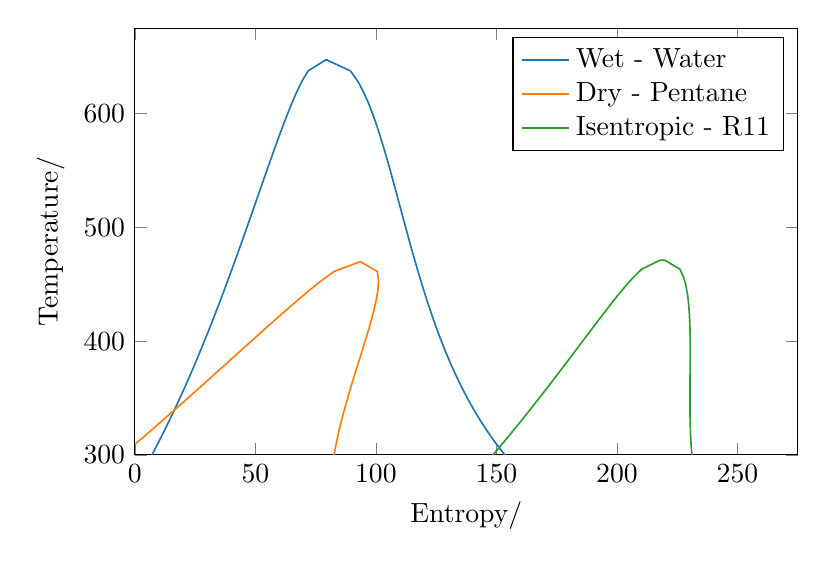
\begin{tikzpicture}

\definecolor{darkgray176}{RGB}{176,176,176}
\definecolor{darkorange25512714}{RGB}{255,127,14}
\definecolor{forestgreen4416044}{RGB}{44,160,44}
\definecolor{lightgray204}{RGB}{204,204,204}
\definecolor{steelblue31119180}{RGB}{31,119,180}

\begin{axis}[
legend cell align={left},
legend style={},
xlabel={Entropy/\unit{\joule\per\mole\per\K}},
xmin=0, xmax=275,
ylabel={Temperature/\unit{\K}},
ymin=300, ymax=675,
width=10cm, height=7cm
]
% \path [draw=red, fill=red, opacity=0.3]
% (axis cs:0,373)
% --(axis cs:300,373)
% --(axis cs:300,573)
% --(axis cs:0,573)
% --(axis cs:0,373)
% --cycle;

\addplot [semithick, steelblue31119180]
table {%
164.938667440739 273.16
160.508880907111 282.748076923077
156.448921690617 292.336153846154
152.719253350367 301.924230769231
149.285183519133 311.512307692308
146.116060741801 321.100384615385
143.184658176851 330.688461538462
140.466679033021 340.276538461539
137.940345620707 349.864615384615
135.586053085874 359.452692307692
133.386080380021 369.040769230769
131.324355112998 378.628846153846
129.386267398397 388.216923076923
127.558523533241 397.805
125.82902651982 407.393076923077
124.186769351259 416.981153846154
122.621729292942 426.569230769231
121.124756098449 436.157307692308
119.687452324709 445.745384615385
118.302047900242 455.333461538462
116.961272887626 464.921538461539
115.658231924154 474.509615384615
114.386281704838 484.097692307692
113.138909810602 493.685769230769
111.909609761842 503.273846153846
110.69174402236 512.861923076923
109.478383961564 522.45
108.262111572081 532.038076923077
107.034759175676 541.626153846154
105.787049808485 551.214230769231
104.508080677342 560.802307692308
103.184554421011 570.390384615384
101.799583857035 579.978461538461
100.330723818017 589.566538461538
98.7464793542399 599.154615384615
96.99946115179 608.742692307692
95.0109488194475 618.330769230769
92.627704013306 627.918846153846
89.4400373125366 637.506923076922
79.6372076401001 647.094999999999
79.155029980754 647.095
71.8729564287978 637.506923076923
69.1914410632728 627.918846153846
67.011976709581 618.330769230769
65.0614494387508 608.742692307693
63.2395253416193 599.154615384616
61.5000511288369 589.566538461539
59.8168046704693 579.978461538462
58.1727571196635 570.390384615385
56.5559530918372 560.802307692308
54.9575449433964 551.214230769231
53.3707024772933 541.626153846154
51.7899537433436 532.038076923078
50.2107648619345 522.450000000001
48.6292617409914 512.861923076924
47.0420397602833 503.273846153847
45.4460297089609 493.68576923077
43.8384005678625 484.097692307693
42.2164868977816 474.509615384616
40.5777329337247 464.921538461539
38.9196481927975 455.333461538462
37.2397711401225 445.745384615385
35.5356386005206 436.157307692308
33.8047593774043 426.569230769232
32.0445910779249 416.981153846155
30.2525195222934 407.393076923078
28.4258403730727 397.805000000001
26.5617427603013 388.216923076924
24.6572946652083 378.628846153847
22.7094295719731 369.04076923077
20.7149332403655 359.452692307693
18.6704281138531 349.864615384616
16.5723504083304 340.276538461539
14.416910624048 330.688461538462
12.2000210129861 321.100384615385
9.9171617201483 311.512307692308
7.5631377847837 301.924230769231
5.13164409329361 292.336153846155
2.61447744080202 282.748076923078
3.14585886081536e-12 273.160000000001
};
\addlegendentry{Wet - Water}
\addplot [semithick, darkorange25512714]
table {%
125.679933116081 143.47
117.352507554121 151.834846153846
110.358531472133 160.199692307692
104.483334026094 168.564538461538
99.5560406263168 176.929384615385
95.4389352262527 185.294230769231
92.0196514153343 193.659076923077
89.2053747596484 202.023923076923
86.9185073484665 210.388769230769
85.0934158087417 218.753615384615
83.6739915295812 227.118461538461
82.6118205113512 235.483307692308
81.8648065873488 243.848153846154
81.3961265165305 252.213
81.1734248831949 260.577846153846
81.1681814257779 268.942692307692
81.3551960323046 277.307538461538
81.7121341433352 285.672384615384
82.2190821627186 294.037230769231
82.8581101941552 302.402076923077
83.6129024704768 310.766923076923
84.4685201142549 319.131769230769
85.4112858239872 327.496615384615
86.428698568638 335.861461538461
87.5092764739641 344.226307692308
88.6422859735569 352.591153846154
89.8173830628884 360.956
91.0242177561756 369.320846153846
92.2520309334678 377.685692307692
93.4892271071156 386.050538461538
94.7228573945467 394.415384615384
95.9378939178915 402.780230769231
97.1160945777997 411.145076923077
98.234082778806 419.509923076923
99.2598413654898 427.874769230769
100.145660140189 436.239615384615
100.811870698277 444.604461538461
101.100545645929 452.969307692307
100.581995448015 461.334153846154
93.62287534686 469.699
93.3522625785748 469.699
82.7545910882402 461.334153846154
77.3003448685538 452.969307692308
72.3712238752941 444.604461538462
67.6767311075994 436.239615384616
63.1129196020519 427.874769230769
58.6285009034989 419.509923076923
54.1935770848717 411.145076923077
49.7887642948912 402.780230769231
45.4004918694483 394.415384615385
41.0186613287295 386.050538461539
36.6353551768051 377.685692307693
32.2440655520643 369.320846153846
27.8392012135916 360.956
23.4157523843684 352.591153846154
18.9690491640705 344.226307692308
14.4945776260239 335.861461538462
9.98783299078754 327.496615384616
5.44419753221384 319.13176923077
0.858834827373093 310.766923076923
-3.77340680564836 302.402076923077
-8.45808884301238 294.037230769231
-13.2012819900779 285.672384615385
-18.0096761015931 277.307538461539
-22.890704046585 268.942692307693
-27.8526812845808 260.577846153847
-32.904962611899 252.213
-38.0581184240851 243.848153846154
-43.3241339914704 235.483307692308
-48.7166360741255 227.118461538462
-54.2511519094982 218.753615384616
-59.9454067540509 210.38876923077
-65.8196682597032 202.023923076923
-71.8971494900635 193.659076923077
-78.2044879113483 185.294230769231
-84.7723259067962 176.929384615385
-91.6360298520966 168.564538461539
-98.8365997650072 160.199692307693
-106.421839645226 151.834846153847
-114.447879450554 143.47
};
\addlegendentry{Dry - Pentane}
\addplot [semithick, forestgreen4416044]
table {%
271.336602927 162.68
265.265066737161 170.587153846154
260.016190656118 178.494307692308
255.475046362461 186.401461538462
251.545442572003 194.308615384615
248.146355515415 202.215769230769
245.20917582829 210.122923076923
242.675517337031 218.030076923077
240.495432497173 225.937230769231
238.625939630814 233.844384615385
237.029803380724 241.751538461538
235.674529920713 249.658692307692
234.531548006255 257.565846153846
233.575550333253 265.473
232.783970307279 273.380153846154
232.13656952992 281.287307692308
231.615112321967 289.194461538462
231.20310577321 297.101615384615
230.88558689713 305.008769230769
230.648941969949 312.915923076923
230.480746521013 320.823076923077
230.369617308507 328.730230769231
230.305069712666 336.637384615385
230.277375186974 344.544538461538
230.277413665174 352.451692307692
230.2965150411 360.358846153846
230.326281804072 368.266
230.358381137632 376.173153846154
230.384288266395 384.080307692308
230.39495154208 391.987461538462
230.380329578589 399.894615384615
230.328712948213 407.801769230769
230.225667879571 415.708923076923
230.052279195911 423.616076923077
229.781995741087 431.523230769231
229.374400141311 439.430384615385
228.761197715945 447.337538461538
227.807783701269 455.244692307692
226.160036323412 463.151846153846
219.855788634981 471.059
217.803202487293 471.059
210.220340559101 463.151846153846
206.4462310651 455.244692307692
203.144744825586 447.337538461538
200.066187239926 439.430384615385
197.108921739116 431.523230769231
194.222311332631 423.616076923077
191.377371018887 415.708923076923
188.555696226728 407.801769230769
185.744614001784 399.894615384615
182.934799444632 391.987461538462
180.118991335045 384.080307692308
177.291246354871 376.173153846154
174.44647818726 368.266
171.580156943458 360.358846153846
168.688103462579 352.451692307692
165.766342047795 344.544538461538
162.810990348029 336.637384615385
159.818173433908 328.730230769231
156.783953939632 320.823076923077
153.704273070622 312.915923076923
150.574899156731 305.008769230769
147.391381727095 297.101615384615
144.149010068976 289.194461538462
140.842776082471 281.287307692308
137.467342078033 273.380153846154
134.017015081003 265.473
130.485730289321 257.565846153846
126.867047647639 249.658692307692
123.154167097404 241.751538461538
119.33996991931 233.844384615385
115.417095533904 225.937230769231
111.378064668506 218.030076923077
107.215459723201 210.122923076923
102.922168762623 202.215769230769
98.4916849510684 194.308615384615
93.9184158428372 186.401461538462
89.1978694960056 178.494307692308
84.3263863104512 170.587153846154
79.299634649923 162.68
};
\addlegendentry{Isentropic - R11}
\end{axis}

\end{tikzpicture}

            \caption{Temperature-Entropy phase envelopes of dry, wet, isentropic fluids. \cite{Babatunde2018}}
            \label{fig:litrev_ORC_working_fluid_types}
        \end{figure}  

         \begin{figure}[H]
            \centering
            % This file was created with tikzplotlib v0.10.1.
\begin{tikzpicture}

\definecolor{crimson2143940}{RGB}{214,39,40}
\definecolor{darkgray176}{RGB}{176,176,176}
\definecolor{darkorange25512714}{RGB}{255,127,14}
\definecolor{forestgreen4416044}{RGB}{44,160,44}
\definecolor{lightgray204}{RGB}{204,204,204}
\definecolor{mediumpurple148103189}{RGB}{148,103,189}
\definecolor{steelblue31119180}{RGB}{31,119,180}

\begin{axis}[
legend cell align={left},
legend style={
  at={(1.03,0.5)},
  anchor=west,
},
xmin=200, xmax=832.307,
xlabel={Critical temperature/\unit{\K}},
ymin=0, ymax=100,
ylabel={Critical pressure/\unit{\bar}},
width=13cm, height=7cm,
% ymode=log
]
\path [draw=red, fill=red, opacity=0.3]
(axis cs:373.15,1000)
--(axis cs:373.15,0)
--(axis cs:573.15,0)
--(axis cs:573.15,1000)
--(axis cs:573.15,1000)
--(axis cs:373.15,1000)
--cycle;

\addplot [semithick, steelblue31119180, mark=*, mark size=3, mark options={solid}, only marks]
table {%
419.29 40.051
562.02 48.94
553.6 40.824
398.3 55.797
511.72 45.712
305.322 48.722
617.12 36.224
282.35 50.418
468.92 73.0468615963585
407.817 36.29
418.09 40.098
497.7 30.4
460.35 33.78
190.564 45.992
433.74 31.96
364.211 45.55
402.38 56.26
591.75 41.26
435.75 42.255
616.89 35.346
425.125 37.96
617.7 21.03
658.1 18.17
540.13 27.36
507.82 30.4411532835969
594.55 22.81
568.74 24.8359119967769
469.7 33.6751899473634
369.89 42.512
638.8 19.904
630.259 37.375
616.168 35.315
428.61 40.273
};
\addlegendentry{Hydrocarbons}
\addplot [semithick, darkorange25512714, mark=*, mark size=3, mark options={solid}, only marks]
table {%
471.06 43.94
487.21 33.922
418.83 32.57
353.1 31.2903696827871
293.03 30.48
385.12 41.361
456.831 36.72
439.6 36.236377763648
367.85 33.822
382.52 36.3493685102173
423.27 35.3061967044966
395.425 36.24295
376.93 35.1786712617843
339.173 36.177
301.88 38.79
374.21 40.5928
396.44 39.5256607171867
227.51 37.5
477.5 42.12
410.26 40.55
345.857 37.61
386.411 45.2
375.25 50.1
451.48 51.812
345.02 26.4
369.295 49.9
374.9 29.2524223394477
299.293 48.32
412.44 34.2
398.07 32
447.57 39.4074048875043
427.01 36.51
351.255 57.82
460 32.6620706788325
416.3 66.7168697714184
345.27 37.348
359.345 46.317
317.28 58.97
344.494 49.012
343.765 37.049
388.38 27.775
450.7 28.49
};
\addlegendentry{Refrigerants}
\addplot [semithick, forestgreen4416044, mark=*, mark size=3, mark options={solid}, only marks]
table {%
586.5 13.4721535609046
618.3 10.7768778025659
645.78 9.61
599.4 11.4402429635701
628 9.53950310236878
653.2 8.28558722066077
564.09 14.1004475581655
518.75 19.39
};
\addlegendentry{Siloxanes}
\addplot [semithick, crimson2143940, mark=*, mark size=3, mark options={solid}, only marks]
table {%
508.1 47
561.6 52.2758510308235
466.7 36.4901689652854
557 49.088
400.378 53.368
514.71 62.68
468.92 73.0468615963585
512.5 82.1585
799 13.41
772 13.69
782 12.46
755 13.5
775 12.39
};
\addlegendentry{Organics}
\addplot [semithick, mediumpurple148103189, mark=*, mark size=3, mark options={solid}, only marks]
table {%
405.4 113.33
304.1282 73.773
132.86 34.94
430.64 78.8658760034641
318.7232 37.54983
647.096 220.64
};
\addlegendentry{Inorganics}
\addplot [semithick, black, mark=diamond*, mark size=4, mark options={solid}, only marks]
table {%
304.1282 73.773
553.6 40.824
398.3 55.797
511.72 45.712
647.096 220.64
425.125 37.96
469.7 33.6751899473634
369.89 42.512
386.411 45.2
374.9 29.2524223394477
};
\addlegendentry{Notables}

\addplot+[mark=none] coordinates {(309.1282,77.46165)} coordinate (CO2);
\addplot+[mark=none] coordinates {(558.6,42.8652)} coordinate (CycloHex);
\addplot+[mark=none] coordinates {(403.3,58.58685)} coordinate (CycloProp);
\addplot+[mark=none] coordinates {(516.72,47.9976)} coordinate (CycloPent);
% \addplot+[mark=none] coordinates {(652.096,231.672)} coordinate (Water);
\addplot+[mark=none] coordinates {(430.125,39.858)} coordinate (Butane);
\addplot+[mark=none] coordinates {(474.7,35.35894)} coordinate (Pentane);
\addplot+[mark=none] coordinates {(364.89,44.6376)} coordinate (Propane);
\addplot+[mark=none] coordinates {(391.411,47.46)} coordinate (R152a);
\addplot+[mark=none] coordinates {(369.9,30.7150434)} coordinate (R227ea);

\end{axis}

\node[scale=0.7,fill=lightgray204, draw=black, line width=0.4pt, inner sep=3pt, rounded corners, anchor=base west, text=black,rotate=0.0] at (CO2) {Carbon Dioxide};
\node[scale=0.7,fill=lightgray204, draw=black, line width=0.4pt, inner sep=3pt, rounded corners, anchor=north west, text=black,rotate=0.0] at (CycloHex) {CycloHexane};
\node[scale=0.7,fill=lightgray204, draw=black, line width=0.4pt, inner sep=3pt, rounded corners, anchor=base west, text=black,rotate=0.0] at (CycloProp) {CycloPropane};
\node[scale=0.7,fill=lightgray204, draw=black, line width=0.4pt, inner sep=3pt, rounded corners, anchor=base west, text=black,rotate=0.0] at (CycloPent) {Cyclopentane};
% \node[scale=0.7,fill=lightgray204, draw=black, line width=0.4pt, inner sep=3pt, rounded corners, anchor=base west, text=black,rotate=0.0] at (Water) {Water};
\node[scale=0.7,fill=lightgray204, draw=black, line width=0.4pt, inner sep=3pt, rounded corners, anchor=base west, text=black,rotate=0.0] at (Butane) {n-Butane};
\node[scale=0.7,fill=lightgray204, draw=black, line width=0.4pt, inner sep=3pt, rounded corners, anchor=north west, text=black,rotate=0.0] at (Pentane) {n-Pentane};
\node[scale=0.7,fill=lightgray204, draw=black, line width=0.4pt, inner sep=3pt, rounded corners, anchor=base east, text=black,rotate=0.0] at (Propane) {n-Propane};
\node[scale=0.7,fill=lightgray204, draw=black, line width=0.4pt, inner sep=3pt, rounded corners, anchor=base west, text=black,rotate=0.0] at (R152a) {R152a};
\node[scale=0.7,fill=lightgray204, draw=black, line width=0.4pt, inner sep=3pt, rounded corners, anchor=base east, text=black,rotate=0.0] at (R227ea) {R227ea};

\end{tikzpicture}
            \caption{Critical temperatures and pressures of various \ac{ORC} working fluids, \cite{Astolfi2014A, Bell2014}}
            \label{fig:litrev_ORC_working_fluids}
        \end{figure}

        \begin{table}[H]
            \caption{Environmental and Health properties of candidate working fluids \cite{DiPippo2016}}
            \centering 
            \label{table:working_fluid_properties}
            \begin{tabular}{|p{3.5cm}|c c c c c c|}
    \hline
    \rowcolor{bluepoli!40} % comment this line to remove the color
    \textbf{Fluid} & \(\mathbf{T_{crit}}\) /\unit{\K} & \textbf{Toxicity} & \textbf{Flammability} & \textbf{ODP} & \textbf{GWP} & \textbf{Banned?} \T\B \\
    \hline \hline
    R-12 & 385.12 & None & None & 1.0 & 4500 & Yes \T\B\\
    R-114 & 418.83 & None & None & 0.7 & 5850 & Yes \T\B\\
    Propane  & 369.89 & Low & Very High & 0 & 3 & No\T\B\\
    i-Butane & 407.81 & Low & Very High & 0 & 3 & No\T\B\\
    n-Butane & 425.125 & Low & Very High & 0 & 3 & No\T\B\\
    i-Pentane & 460.35 & Low & Very High & 0 & 3 & No\T\B\\
    n-Pentane & 469.70 & Low & Very High & 0 & 3 & No\T\B\\
    R-32 & 351.26 & Very Low & Low & 0 & 675 & No\T\B\\
    R-134a & 374.21 & Very Low & None & 0 & 1300 & No\T\B\\
    R-245fa & 427.01 & Low & None & 0 & 1020 & No\T\B\\
    %  & 427.01 & Low & None & 0 & 1020 & No\T\B\\
    % Neopentane & 427.01 & Low & None & 0 & 1020 & No\T\B\\
    % Isohexane & 427.01 & Low & None & 0 & 1020 & No\T\B\\
    % Hexane & 427.01 & Low & None & 0 & 1020 & No\T\B\\
    % Heptane & 427.01 & Low & None & 0 & 1020 & No\T\B\\
    % Octane & 427.01 & Low & None & 0 & 1020 & No\T\B\\
    % Nonane & 427.01 & Low & None & 0 & 1020 & No\T\B\\
    % Decane& 427.01 & Low & None & 0 & 1020 & No\T\B\\
    % Cyclopropane& 427.01 & Low & None & 0 & 1020 & No\T\B\\
    % Cyclopentane& 427.01 & Low & None & 0 & 1020 & No\T\B\\
    % Cyclohexane& 427.01 & Low & None & 0 & 1020 & No\T\B\\
    % Methylcyclohexane & 427.01 & Low & None & 0 & 1020 & No\T\B\\
    % Propylcyclohexane& 427.01 & Low & None & 0 & 1020 & No\T\B\\
    % Isobutene& 427.01 & Low & None & 0 & 1020 & No\T\B\\
    % 1-Butene& 427.01 & Low & None & 0 & 1020 & No\T\B\\
    % Trans-Butene& 427.01 & Low & None & 0 & 1020 & No\T\B\\
    % Cis-Butene& 427.01 & Low & None & 0 & 1020 & No\T\B\\
    % Benzene& 427.01 & Low & None & 0 & 1020 & No\T\B\\
    % Propyne& 427.01 & Low & None & 0 & 1020 & No\T\B\\
    % Methanol& 427.01 & Low & None & 0 & 1020 & No\T\B\\
    % Ethanol& 427.01 & Low & None & 0 & 1020 & No\T\B\\
    % Toluene & 427.01 & Low & None & 0 & 1020 & No\T\B\\
    % Acetone & 427.01 & Low & None & 0 & 1020 & No\T\B\\
    % Dimethylether & 427.01 & Low & None & 0 & 1020 & No\T\B\\
    % R125 & 427.01 & Low & None & 0 & 1020 & No\T\B\\
    % R143a & 427.01 & Low & None & 0 & 1020 & No\T\B\\
    % R1234yf & 427.01 & Low & None & 0 & 1020 & No\T\B\\
    % R227ea & 427.01 & Low & None & 0 & 1020 & No\T\B\\
    % R161 & 427.01 & Low & None & 0 & 1020 & No\T\B\\
    % R1234ze & 427.01 & Low & None & 0 & 1020 & No\T\B\\
    % R152a & 427.01 & Low & None & 0 & 1020 & No\T\B\\
    % R236fa & 427.01 & Low & None & 0 & 1020 & No\T\B\\
    % R236ea & 427.01 & Low & None & 0 & 1020 & No\T\B\\
    % R245fa & 427.01 & Low & None & 0 & 1020 & No\T\B\\
    % R365mfc & 427.01 & Low & None & 0 & 1020 & No\T\B\\
    % R218 & 427.01 & Low & None & 0 & 1020 & No\T\B\\
    % RC318 & 427.01 & Low & None & 0 & 1020 & No\T\B\\
    % MM & 427.01 & Low & None & 0 & 1020 & No\T\B\\
    % Mdm & 427.01 & Low & None & 0 & 1020 & No\T\B\\
    % Md2m & 427.01 & Low & None & 0 & 1020 & No\T\B\\
    % Md3m & 427.01 & Low & None & 0 & 1020 & No\T\B\\
    % Md4m & 427.01 & Low & None & 0 & 1020 & No\T\B\\
    % D4 & 427.01 & Low & None & 0 & 1020 & No\T\B\\
    % D5 & 427.01 & Low & None & 0 & 1020 & No\T\B\\
    % D6 & 427.01 & Low & None & 0 & 1020 & No\T\B\\
    % Ammonia & 427.01 & Low & None & 0 & 1020 & No\T\B\\
    % Water & 427.01 & Low & None & 0 & 1020 & No\T\B\\    
    \hline
\end{tabular}
        
            \\[10pt]
        \end{table}
        
    \subsection{Configurations}
        The following section aims to provide background on the different strategies used to increase the efficiency of \ac{ORC}s

        \subsubsection{Recuperative Cycle}
            Where the turbine exhaust has a sufficiently high temperature, it can be used to pre-heat the pressurised working fluid before entering the pre-heater, Figure~\ref{fig:litrev_ORC_recu_schematic}. This has two main advantages: 1) reducing the duty and thus size and cost of the condenser; and 2) reducing the duty of the \ac{PHE}, which can be of operational importance when handling geofluids prone to scaling at lower temperatures, also see Section~\ref{sec:litrev_scale_handling}.

             \begin{figure}[H]
                \centering
                % \resizebox{.75\linewidth}{!}{\begin{tikzpicture}
    % draw equipment
    \pic (producer) at (0,0) {producer};
    \pic (injector) at (2,0) {injector};
    \pic[rotate=180] (evap) at ($(injector-anchor) + (0.925, 4)$) {heat exchanger biphase};
    \pic[rotate=180] (preh) at ($(evap-anchor) + (0, -1.5)$) {heat exchanger biphase};
    \pic (solids) [scale=0.25] at ($(evap-pipes bottom) + (-1.5, 0)$) {block};
    \pic (turbine) at ($(evap-anchor) + (4.5, 0)$) {turbine_gen};
    \pic (recuperator) at ($(turbine-outlet bottom) + (0, -2)$) {heat exchanger};
    \pic[rotate=270] (condenser) at ($(recuperator-anchor) + (1.5, -1.5)$) {heat exchanger biphase};
    \pic (pump) at ($(condenser-anchor) + (1.5, 1.1)$) {centrifugal pump};
    
    % % draw connectors
    \draw[main stream] (producer-top) |- (solids-left);
    \draw[main stream] (solids-right) -- (evap-pipes bottom);
    \draw[main stream] (solids-bottom) -- ++ (0, -0.5);
    \draw[main stream] (evap-pipes top) 
        -| ($(evap-pipes top) + (-0.5, -1)$) 
        -- (preh-pipes bottom);
    \draw[main stream] (preh-pipes top) 
        -| ($(preh-pipes top) + (-0.5, -1)$) 
        -- (injector-top);
    \draw[main stream] (evap-shell bottom) |- ++ (0, 0.2) -| (turbine-inlet top);
    \draw[main stream] (turbine-outlet bottom) -- (recuperator-shell top);
    \draw[main stream] (recuperator-shell bottom) |- (condenser-shell bottom);
    \draw[main stream] (condenser-shell top) -| ++ (0.3, 0.3) |- (pump-anchor);
    \draw[main stream] (pump-top) -- (recuperator-pipes right);
    \draw[main stream] (recuperator-pipes left) -| (preh-shell top);
    \draw[main stream] (preh-shell bottom) -| (evap-shell top);
    \draw[main stream] (condenser-pipes bottom) -- ++ (0,-1);
    \draw[main stream] ($(condenser-pipes top) + (0, -1)$) -- (condenser-pipes top);
    
    
    % % draw labels
    \node[above, align=center] at (solids-top) {Solids\\Removal};
    \node[below] at (producer-bottom) {Producer};
    % \node[right] at (preheater-shell left) {Pre-Heater};
    \node[right] at (evap-shell left) {Evaporator};
    % \node[right] at (superheater-shell left) {Super-Heater};
    \node[above] at ($(turbine-top)+ (0.5,0.1)$) {Turbine};
    \node[right] at (turbine-right) {Generator};
    \node[right, align=left] at ($(recuperator-anchor) + (0.5, 0.5)$) {Recuperator};
    \node[left, align=left] at ($(condenser-anchor) + (-0.5, -0.5)$) {Condenser};
    \node[right, align=center] at (pump-right) {Circulation \\ Pump};
    \node[below] at (injector-bottom) {Injector};
    \node[right, align=left] at ($(condenser-pipes top) + (0, -1)$) {Coolant in};
    \node[left, align=left] at ($(condenser-pipes bottom) + (0, -1)$) {Coolant out};
    
\end{tikzpicture}}
                \begin{tikzpicture}
    % draw equipment
    \pic (producer) at (0,0) {producer};
    \pic (injector) at (2,0) {injector};
    \pic[rotate=180] (evap) at ($(injector-anchor) + (0.925, 4)$) {heat exchanger biphase};
    \pic[rotate=180] (preh) at ($(evap-anchor) + (0, -1.5)$) {heat exchanger biphase};
    \pic (solids) [scale=0.25] at ($(evap-pipes bottom) + (-1.5, 0)$) {block};
    \pic (turbine) at ($(evap-anchor) + (4.5, 0)$) {turbine_gen};
    \pic (recuperator) at ($(turbine-outlet bottom) + (0, -2)$) {heat exchanger};
    \pic[rotate=270] (condenser) at ($(recuperator-anchor) + (1.5, -1.5)$) {heat exchanger biphase};
    \pic (pump) at ($(condenser-anchor) + (1.5, 1.1)$) {centrifugal pump};
    
    % % draw connectors
    \draw[main stream] (producer-top) |- (solids-left);
    \draw[main stream] (solids-right) -- (evap-pipes bottom);
    \draw[main stream] (solids-bottom) -- ++ (0, -0.5);
    \draw[main stream] (evap-pipes top) 
        -| ($(evap-pipes top) + (-0.5, -1)$) 
        -- (preh-pipes bottom);
    \draw[main stream] (preh-pipes top) 
        -| ($(preh-pipes top) + (-0.5, -1)$) 
        -- (injector-top);
    \draw[main stream] (evap-shell bottom) |- ++ (0, 0.2) -| (turbine-inlet top);
    \draw[main stream] (turbine-outlet bottom) -- (recuperator-shell top);
    \draw[main stream] (recuperator-shell bottom) |- (condenser-shell bottom);
    \draw[main stream] (condenser-shell top) -| ++ (0.3, 0.3) |- (pump-anchor);
    \draw[main stream] (pump-top) -- (recuperator-pipes right);
    \draw[main stream] (recuperator-pipes left) -| (preh-shell top);
    \draw[main stream] (preh-shell bottom) -| (evap-shell top);
    \draw[main stream] (condenser-pipes bottom) -- ++ (0,-1);
    \draw[main stream] ($(condenser-pipes top) + (0, -1)$) -- (condenser-pipes top);
    
    
    % % draw labels
    \node[above, align=center] at (solids-top) {Solids\\Removal};
    \node[below] at (producer-bottom) {Producer};
    % \node[right] at (preheater-shell left) {Pre-Heater};
    \node[right] at (evap-shell left) {Evaporator};
    % \node[right] at (superheater-shell left) {Super-Heater};
    \node[above] at ($(turbine-top)+ (0.5,0.1)$) {Turbine};
    \node[right] at (turbine-right) {Generator};
    \node[right, align=left] at ($(recuperator-anchor) + (0.5, 0.5)$) {Recuperator};
    \node[left, align=left] at ($(condenser-anchor) + (-0.5, -0.5)$) {Condenser};
    \node[right, align=center] at (pump-right) {Circulation \\ Pump};
    \node[below] at (injector-bottom) {Injector};
    \node[right, align=left] at ($(condenser-pipes top) + (0, -1)$) {Coolant in};
    \node[left, align=left] at ($(condenser-pipes bottom) + (0, -1)$) {Coolant out};
    
\end{tikzpicture}
                \caption[Schematic of a binary ORC geothermal power plant with recuperation.]{Schematic of a binary ORC geothermal power plant with recuperation. Adapted from \cite{DiPippo2016}}
                \label{fig:litrev_ORC_recu_schematic}
            \end{figure}
    
             \begin{figure}[H]
                \centering
                % This file was created with tikzplotlib v0.10.1.
\begin{tikzpicture}

\definecolor{darkgray176}{RGB}{176,176,176}
\definecolor{darkorange25512714}{RGB}{255,127,14}
\definecolor{lightgray204}{RGB}{204,204,204}
\definecolor{steelblue31119180}{RGB}{31,119,180}

\begin{groupplot}[group style={group size=2 by 1}, width=7.5cm, height=7cm]
\nextgroupplot[
xlabel={Entropy/\unit{\kilo\joule\per\kg}},
xmin=0, xmax=1.5,
ylabel={Temperature/\unit{\K}},
ymin=300, ymax=450,
]
\addplot [semithick, black, dotted]
table {%
2.00514604740525 134.895
1.8742645647399 142.336769230769
1.76279255666379 149.778538461538
1.66768401333555 157.220307692308
1.5864785704731 164.662076923077
1.51716884301893 172.103846153846
1.45810097682024 179.545615384615
1.40789947437052 186.987384615385
1.36541000440908 194.429153846154
1.32965565464722 201.870923076923
1.29980327418206 209.312692307692
1.27513739100831 216.754461538462
1.25503980788016 224.196230769231
1.23897345092445 231.638
1.22646940618215 239.079769230769
1.2171163590369 246.521538461539
1.21055185951343 253.963307692308
1.20645499128141 261.405076923077
1.20454013215318 268.846846153846
1.20455157032991 276.288615384616
1.20625879260282 283.730384615385
1.20945229302806 291.172153846154
1.21393977050186 298.613923076923
1.21954259643317 306.055692307692
1.22609246268062 313.497461538462
1.23342816828847 320.939230769231
1.24139235873288 328.381
1.24982725696202 335.822769230769
1.25856758042055 343.264538461539
1.26743010117866 350.706307692308
1.27620257808655 358.148076923077
1.28463483166039 365.589846153846
1.29242817432022 373.031615384616
1.29921104595928 380.473384615385
1.30448309491165 387.915153846154
1.30749842859047 395.356923076923
1.30700810774302 402.798692307693
1.30055851246937 410.240461538462
1.28162083881394 417.682230769231
1.15438324302955 425.124
0.992479179474436 417.682230769231
0.915542659182493 410.240461538462
0.847302498583098 402.798692307692
0.782886125906925 395.356923076923
0.720594996479248 387.915153846154
0.659615405298665 380.473384615385
0.599483713195194 373.031615384615
0.53990313387527 365.589846153846
0.480666335398733 358.148076923077
0.421617964817889 350.706307692308
0.36263460385308 343.264538461538
0.303613141549675 335.822769230769
0.244463538471646 328.381
0.185104036650966 320.939230769231
0.125457802932702 313.497461538461
0.0654504419025093 306.055692307692
0.00500804765388449 298.613923076923
};
\addplot [semithick, steelblue31119180, dashed]
table {%
1.30689960935835 393.150000000765
1.30689960935835 328.196001431158
};
\addplot [semithick, black, dashed]
table {%
0.14098139885952 316.344229994678
1.25783715965587 320.000000000024
};
\addplot [semithick, black, dashed]
table {%
0.233973781167455 328.010780652277
1.34927443812995 335.369806025193
};
\addplot [semithick, steelblue31119180, mark=*, mark size=3, mark options={solid}]
table {%
0.137527453172052 315
0.14098139885952 316.344229994678
0.233973781167455 328.010780652277
0.764238028852845 393.150000000765
1.30689960935846 393.150000000765
1.34927443812995 335.369806025193
1.25783715965587 320.000000000024
1.22751538416118 315.000000000024
0.137527453172243 315.000000000024
};

\nextgroupplot[
legend cell align={left},
legend style={
  at={(0.03,0.97)},
  anchor=north west,
},
xlabel={Heat Transferred/\unit{\kilo\watt\per\kg\s}},
xmin=0, xmax=325,
ymin=300, ymax=443.15,
ymajorticks=false,
]
\addplot [semithick, darkorange25512714]
table {%
21.0825908599491 366.270067513618
305.97092373671 433.15
};
\addlegendentry{Geofluid}
\addplot [semithick, steelblue31119180]
table {%
0 316.344229994678
21.0825908599491 328.010780652277
155.837624860223 393.150000000765
305.97092373671 393.150000000765
};
\addlegendentry{n-Butane}
\addplot [semithick, black, dashed, forget plot]
table {%
0 316.344229994678
248.388474151653 320.000000000024
};
\addplot [semithick, black, dashed, forget plot]
table {%
21.0825908599491 328.010780652277
269.4710650116 335.369806025193
};
\addplot [semithick, steelblue31119180, forget plot]
table {%
0 315
241.613899727913 315.000000000024
248.388474151653 320.000000000024
269.4710650116 335.369806025193
};
\end{groupplot}

\begin{groupplot}[group style={group size=2 by 1}, width=7.5cm, height=7cm]
\nextgroupplot[
axis y line=none,
axis x line=none,
xmajorticks=false,
ymajorticks=false
]
\nextgroupplot[
axis x line=none,
axis y line=right,
tick align=outside,
xmin=0, xmax=325,
ylabel={Temperature/\unit{\degreeCelsius}},
ymin=27, ymax=170.15,
xmajorticks=false
]
\end{groupplot}

\end{tikzpicture}

                \caption[TS and TQ diagrams of a recuperative binary \ac{ORC} using n-Butane as the working fluid.]{Temperature-Entropy and Temperature-Heat transfer diagrams of a recuperative binary \ac{ORC} geothermal power plant using n-Butane as the working fluids for a saturated water-dominated geofluid at a temperature of \qty{433}{\K} (\qty{160}{\degreeCelsius}) at the inlet. The cycle parameters were not optimised.}
                \label{fig:litrev_ORC_recu_TS}
            \end{figure}
    
        % \textbf{Turbine Bleeding}\\
        % Similarly to a recuperative cycle, working fluid may also be prematurely bled from the turbine and mixed with the partially pressurised working fluid, Figure~\ref{fig:litrev_ORC_turb_bleeding_schematic}, reducing the duty of the primary heat exchange unit.

        %  \begin{figure}[H]
        %     \centering
        %     \begin{tikzpicture}
    % draw equipment
    \pic (producer) at (0,0) {producer};
    \pic (injector) at (2,0) {injector};
    \pic[rotate=180] (evap) at ($(injector-anchor) + (0.925, 4)$) {heat exchanger biphase};
    \pic[rotate=180] (preh) at ($(evap-anchor) + (0, -1.5)$) {heat exchanger biphase};
    \pic (solids) [scale=0.25] at ($(evap-pipes bottom) + (-1.5, 0)$) {block};
    \pic (turbine) at ($(evap-anchor) + (5.5, 0)$) {turbine_gen};
    \pic (condenser) at ($(turbine-outlet bottom) + (0, -1.6)$) {heat exchanger biphase};
    \pic (lppump) at ($(condenser-anchor) + (-1.5, -1)$) {centrifugal pump};
    \pic (hppump) at ($(lppump-top) + (-3, 0)$) {centrifugal pump};
    \pic (mix) at ($(lppump-top) + (-1.5, 0)$) {valve triple=main};
    
    % % draw connectors
    \draw[main stream] (producer-top) |- (solids-left);
    \draw[main stream] (solids-right) -- (evap-pipes bottom);
    \draw[main stream] (solids-bottom) -- ++ (0, -0.5);
    \draw[main stream] (evap-pipes top) 
        -| ($(evap-pipes top) + (-0.5, -1)$) 
        -- (preh-pipes bottom);
    \draw[main stream] (preh-pipes top) 
        -| ($(preh-pipes top) + (-0.5, -1)$) 
        -- (injector-top);
    \draw[main stream] (evap-shell bottom) |- ++ (0, 0.2) -| (turbine-inlet top);
    \draw[main stream] (turbine-outlet bottom) -- (condenser-shell top);
    \draw[main stream] (condenser-shell bottom) |- (lppump-anchor);
    \draw[main stream] (lppump-top) -- (mix-right);
    \draw[main stream] (mix-left) -- (hppump-anchor);
    \draw[main stream] (hppump-top) -| (preh-shell top);
    \draw[main stream] ($0.5*(turbine-inlet bottom) + 0.5*(turbine-outlet bottom)$) |- ++(-1,-1) -| (mix-top);
    \draw[main stream] (preh-shell bottom) -| (evap-shell top);
    \draw[main stream] (condenser-pipes top) -- ++ (1,0);
    \draw[main stream] ($(condenser-pipes bottom) + (1, 0)$) -- (condenser-pipes bottom);
    
    
    % % draw labels
    \node[above, align=center] at (solids-top) {Solids\\Removal};
    \node[below] at (producer-bottom) {Producer};
    \node[right] at (evap-shell left) {Evaporator};
    \node[right] at (preh-shell left) {Pre-Heater};
    \node[above] at ($(turbine-top)+ (0.5,0.1)$) {Turbine};
    \node[right] at (turbine-right) {Generator};
    \node[left, align=left] at (condenser-shell left) {Condenser};
    \node[below, align=center] at (lppump-bottom) {LP Pump};
    \node[below] at (injector-bottom) {Injector};
    \node[right, align=left] at ($(condenser-pipes bottom) + (1, 0)$) {Coolant in};
    \node[right, align=left] at ($(condenser-pipes top) + (1, 0)$) {Coolant out};
    
\end{tikzpicture}
        %     \caption{Schematic of a binary ORC geothermal power plant with recuperation.}
        %     \label{fig:litrev_ORC_turb_bleeding_schematic}
        % \end{figure}        
        
        \subsubsection{Double Pressure}
            In double pressure cycles evaporation occurs at two distinct pressure levels, an intermediate pressure and a high pressure. In this configuration, the low-pressure working fluid is pressurised to the intermediate pressure and then pre-heated to its boiling point, Figure~\ref{fig:litrev_ORC_dualP_schematic}. The working fluid is then split into two streams, one is vaporised and sent to the turbine while the other is pressurised to a higher pressure, thus raising its boiling point, before being vaporised and then sent to the turbine. The streams can then either be expanded in two separate turbines or using a dual-inlet turbine.
        
             \begin{figure}[H]
                \centering
                % \begin{tikzpicture}

%     \pic (producer) at (0,0) {producer};
%     \pic (injector) at (4,0) {injector};

%     \pic[rotate=180] (hpevap) at ($(injector-anchor) + (1, 6)$) {heat exchanger biphase};
%     \pic[rotate=180] (hppreh) at ($(hpevap-anchor) + (0, -1.5)$) {heat exchanger biphase};
%     \pic (solids) [scale=0.25] at ($(hpevap-pipes bottom) + (-3.5, 0)$) {block};

%     \pic (lpevap) at ($(hpevap-anchor) + (-2.5, -0.5)$) {heat exchanger biphase};
%     \pic (lppreh) at ($(lpevap-anchor) + (0, -3.5)$) {heat exchanger biphase};

%     \pic[rotate=-90] (split) at ($(hppreh-pipes bottom) + (-1, 0)$) {valve triple=main};
%     \pic[rotate=90] (mix) at ($(lppreh-pipes bottom) + (1.07, 0)$) {valve triple=main};
%     \pic[rotate=-90] (split2) at ($(lppreh-shell top) + (0, 0.5)$) {valve triple=main};

%     \pic (turbine) at ($(hpevap-anchor) + (3.5, 0)$) {multi_turbine_gen};
%     \pic (condenser) at ($(turbine-outlet_lp bottom) + (0, -3.5)$) {heat exchanger biphase};
%     \pic (lppump) at ($(condenser-anchor) + (-2, -1.3)$) {centrifugal pump};
%     \pic (hppump) at ($(split2-anchor) + (2.5, 0)$) {centrifugal pump};

%     \draw[main stream] (producer-top) |- (solids-left);
%     \draw[main stream] (solids-bottom) -- ++ (0, -0.5);
%     \draw[main stream] (solids-right) -- (hpevap-pipes bottom);
%     \draw[main stream] (hpevap-pipes top) -- (lpevap-pipes top);

%     \draw[main stream] (lpevap-pipes bottom) -| (split-left);
%     \draw[main stream] (split-top) |- (hppreh-pipes bottom);
%     \draw[main stream] (split-right) |- (lppreh-pipes top);

%     \draw[main stream] (lppreh-pipes bottom) -- (mix-top);
%     \draw[main stream] (hppreh-pipes top) -| (mix-right);
%     \draw[main stream] (mix-left) -- (injector-top);

%     \draw[main stream] (condenser-shell bottom) |- (lppump-anchor);
%     \draw[main stream] (lppump-top) -| (lppreh-shell bottom);
%     \draw[main stream] (lppreh-shell top) -- (split2-right);
%     \draw[main stream] (split2-top) -- (hppump-anchor);
%     \draw[main stream] (hppump-top) -- (hppreh-shell top);
%     \draw[main stream] (hppreh-shell bottom) -- (hpevap-shell top);
%     \draw[main stream] (split2-left) -- (lpevap-shell bottom);

%     \draw[main stream] (hpevap-shell bottom) |- ++ (0.3, 0.3) -| (turbine-inlet_hp top);
%     \draw[main stream] (lpevap-shell top) |- ++ (1.2, 1.2) -| (turbine-inlet_lp top);
%     \draw[main stream] (turbine-outlet_lp bottom) -- (condenser-shell top);

%     \draw[main stream] (condenser-pipes top) -- ++ (1,0);
%     \draw[main stream] ($(condenser-pipes bottom) + (1, 0)$) -- (condenser-pipes bottom);

%     \node[below] at (producer-bottom) {Producer};
%     \node[below] at (injector-bottom) {Injector};
%     \node[above, align=center] at (solids-top) {Solids\\Removal};
%     \node[right] at (hpevap-shell left) {HP Evap.};
%     \node[right] at (hppreh-shell left) {HP Pre-H.};
%     \node[left] at ($(lpevap-shell bottom) + (-0.3, 0)$) {LP Evap.};
%     \node[left] at ($(lppreh-shell bottom) + (-0.3, 0)$) {LP Pre-H.};
%     \node[right, align=left] at ($(condenser-pipes bottom) + (1, 0)$) {Coolant in};
%     \node[right, align=left] at ($(condenser-pipes top) + (1, 0)$) {Coolant out};
%     \node[below] at ($(hppump-bottom) + (0.3, 0)$) {HP Pump};
%     \node[below] at (lppump-bottom) {LP Pump};

%     \node[above] at ($(turbine-top)+ (1,0.1)$) {Turbine};
%     \node[right] at (turbine-right) {Generator};
% \end{tikzpicture}

\begin{tikzpicture}

    \pic (producer) at (0,0) {producer};
    \pic (injector) at (4,0) {injector};

    \pic[rotate=180] (hpevap) at ($(injector-anchor) + (1, 6)$) {heat exchanger biphase};
    \pic[rotate=180] (hppreh) at ($(hpevap-anchor) + (0, -1.5)$) {heat exchanger biphase};
    \pic (solids) [scale=0.25] at ($(hpevap-pipes bottom) + (-3.5, 0)$) {block};

    \pic (lpevap) at ($(hppreh-anchor) + (-2.5, -0.5)$) {heat exchanger biphase};
    \pic (lppreh) at ($(lpevap-anchor) + (0, -2)$) {heat exchanger biphase};

    \pic[rotate=-90] (split2) at ($(lppreh-shell top) + (0, 0.5)$) {valve triple=main};

    \pic (turbine) at ($(hpevap-anchor) + (3.5, 0)$) {multi_turbine_gen};
    \pic (condenser) at ($(turbine-outlet_lp bottom) + (0, -3.5)$) {heat exchanger biphase};
    \pic (lppump) at ($(condenser-anchor) + (-2, -1.3)$) {centrifugal pump};
    \pic (hppump) at ($(split2-anchor) + (2.5, 0)$) {centrifugal pump};

    \draw[main stream] (producer-top) |- (solids-left);
    \draw[main stream] (solids-bottom) -- ++ (0, -0.5);
    \draw[main stream] (solids-right) -- (hpevap-pipes bottom);
    \draw[main stream] (hpevap-pipes top) -| ++ (-0.5, -0.5) |- (hppreh-pipes bottom);  
    \draw[main stream] (hppreh-pipes top) -- (lpevap-pipes top);
    \draw[main stream] (lpevap-pipes bottom) -| ++ (0.5, -0.5) |- (lppreh-pipes top);

    \draw[main stream] (lppreh-pipes bottom) -| (injector-top);

    \draw[main stream] (condenser-shell bottom) |- (lppump-anchor);
    \draw[main stream] (lppump-top) -| (lppreh-shell bottom);
    \draw[main stream] (lppreh-shell top) -- (split2-right);
    \draw[main stream] (split2-top) -- (hppump-anchor);
    \draw[main stream] (hppump-top) -- (hppreh-shell top);
    \draw[main stream] (hppreh-shell bottom) -- (hpevap-shell top);
    \draw[main stream] (split2-left) -- (lpevap-shell bottom);

    \draw[main stream] (hpevap-shell bottom) |- ++ (0.3, 0.3) -| (turbine-inlet_hp top);
    \draw[main stream] (lpevap-shell top) |- ++ (3, 2.7) -| (turbine-inlet_lp top);
    \draw[main stream] (turbine-outlet_lp bottom) -- (condenser-shell top);

    \draw[main stream] (condenser-pipes top) -- ++ (1,0);
    \draw[main stream] ($(condenser-pipes bottom) + (1, 0)$) -- (condenser-pipes bottom);

    \node[below] at (producer-bottom) {Producer};
    \node[below] at (injector-bottom) {Injector};
    \node[above, align=center] at (solids-top) {Solids\\Removal};
    \node[right] at (hpevap-shell left) {HP Evap.};
    \node[right] at (hppreh-shell left) {HP Pre-H.};
    \node[left] at ($(lpevap-shell bottom) + (-0.3, 0)$) {LP Evap.};
    \node[left] at ($(lppreh-shell bottom) + (-0.3, 0)$) {LP Pre-H.};
    \node[right, align=left] at ($(condenser-pipes bottom) + (1, 0)$) {Coolant in};
    \node[right, align=left] at ($(condenser-pipes top) + (1, 0)$) {Coolant out};
    \node[below] at ($(hppump-bottom) + (0.3, 0)$) {HP Pump};
    \node[below] at (lppump-bottom) {LP Pump};

    \node[above] at ($(turbine-top)+ (1,0.1)$) {Turbine};
    \node[right] at (turbine-right) {Generator};
\end{tikzpicture}
                \caption[Schematic of a double pressure binary ORC geothermal power plant.]{Schematic of a double pressure binary ORC geothermal power plant. Adapted from \cite{DiPippo2016}}
                \label{fig:litrev_ORC_dualP_schematic}
            \end{figure}
            % \todo{I dont think the first version of the dualP diagram is correct... it is taken from DiPippo, but I struggle to see how this would be sensible}
    
            The use of double- or multi-pressure cycles has the advantage of obtaining a closer match between the heat profiles of the geofluid and the cycle working fluid in the \ac{PHE}, see Figure~\ref{fig:litrev_ORC_dualP_TS}, reducing exergetic losses and raising the cycle efficiency.         

             \begin{figure}[H]
                \centering
                % This file was created with tikzplotlib v0.10.1.
\begin{tikzpicture}

\definecolor{darkgray176}{RGB}{176,176,176}
\definecolor{darkorange25512714}{RGB}{255,127,14}
\definecolor{lightgray204}{RGB}{204,204,204}
\definecolor{steelblue31119180}{RGB}{31,119,180}

\begin{groupplot}[group style={group size=2 by 1}, width=7.5cm, height=7cm]
\nextgroupplot[
unbounded coords=jump,
xlabel={Entropy/\unit{\kilo\joule\per\kg\per\K}},
xmin=0, xmax=1.5,
ylabel={Temperature/\unit{\K}},
ymin=300, ymax=450,
]
\addplot [semithick, steelblue31119180, mark=*, mark size=3, mark options={solid}]
table {%
0.137527453172052 315
0.140285166509269 316.074569976674
0.681431097875723 383.149999999999
1.30131322777442 383.149999999999
1.30994767491432 384.321748511886
1.34837577744318 335.21681849222
1.22751538416118 315.000000000024
0.137527453172243 315.000000000024
nan nan
0.682951789840748 384.363981609818
0.850418413734198 403.15
1.30686515330246 403.15
1.31347442092921 384.804364635514
};
\addplot [semithick, steelblue31119180, dashed]
table {%
1.30994767491418 384.321748511886
1.30994767491418 328.70920549477
nan nan
1.30686515330246 403.15
1.30686515330246 383.90181095162
};
\addplot [semithick, black, dotted]
table {%
2.00514604740525 134.895
1.8742645647399 142.336769230769
1.76279255666379 149.778538461538
1.66768401333555 157.220307692308
1.5864785704731 164.662076923077
1.51716884301893 172.103846153846
1.45810097682024 179.545615384615
1.40789947437052 186.987384615385
1.36541000440908 194.429153846154
1.32965565464722 201.870923076923
1.29980327418206 209.312692307692
1.27513739100831 216.754461538462
1.25503980788016 224.196230769231
1.23897345092445 231.638
1.22646940618215 239.079769230769
1.2171163590369 246.521538461539
1.21055185951343 253.963307692308
1.20645499128141 261.405076923077
1.20454013215318 268.846846153846
1.20455157032991 276.288615384616
1.20625879260282 283.730384615385
1.20945229302806 291.172153846154
1.21393977050186 298.613923076923
1.21954259643317 306.055692307692
1.22609246268062 313.497461538462
1.23342816828847 320.939230769231
1.24139235873288 328.381
1.24982725696202 335.822769230769
1.25856758042055 343.264538461539
1.26743010117866 350.706307692308
1.27620257808655 358.148076923077
1.28463483166039 365.589846153846
1.29242817432022 373.031615384616
1.29921104595928 380.473384615385
1.30448309491165 387.915153846154
1.30749842859047 395.356923076923
1.30700810774302 402.798692307693
1.30055851246937 410.240461538462
1.28162083881394 417.682230769231
1.15438324302955 425.124
0.992479179474436 417.682230769231
0.915542659182493 410.240461538462
0.847302498583098 402.798692307692
0.782886125906925 395.356923076923
0.720594996479248 387.915153846154
0.659615405298665 380.473384615385
0.599483713195194 373.031615384615
0.53990313387527 365.589846153846
0.480666335398733 358.148076923077
0.421617964817889 350.706307692308
0.36263460385308 343.264538461538
0.303613141549675 335.822769230769
0.244463538471646 328.381
0.185104036650966 320.939230769231
0.125457802932702 313.497461538461
0.0654504419025093 306.055692307692
0.00500804765388449 298.613923076923
-0.0559444080336213 291.172153846154
-0.117484480442669 283.730384615384
-0.179693535821323 276.288615384615
-0.242657974334995 268.846846153846
-0.306470435530277 261.405076923077
-0.37123101948694 253.963307692308
-0.437048550534185 246.521538461538
-0.504041906866955 239.079769230769
-0.572341437975566 231.638
-0.642090492250023 224.196230769231
-0.713447079497475 216.754461538461
-0.786585697741913 209.312692307692
-0.861699361144793 201.870923076923
-0.939001877036892 194.429153846154
-1.01873043594029 186.987384615384
-1.10114860017815 179.545615384615
-1.18654980484172 172.103846153846
-1.27526151837439 164.662076923077
-1.36765024289883 157.220307692307
-1.46412754891255 149.778538461538
-1.56515728978446 142.336769230769
};

\nextgroupplot[
legend cell align={left},
legend style={
  at={(0.03,0.97)},
  anchor=north west,
},
unbounded coords=jump,
xlabel={Heat Transferred/\unit{\kilo\watt\per\kg\s}},
xmin=0, xmax=350,
ymin=300, ymax=450,
ymajorticks=false
]
\addplot [semithick, darkorange25512714]
table {%
0 353.020970051211
340.548113520954 433.15
};
\addlegendentry{Geofluid}
\addplot [semithick, steelblue31119180]
table {%
0 316.074569976674
147.989258398714 383.149999999999
201.820868511941 383.149999999999
nan nan
201.820868511941 384.363981609818
238.4361687695 403.15
340.548113520954 403.15
};
\addlegendentry{n-Butane}
\addplot [semithick, steelblue31119180, forget plot]
table {%
0 315
265.621623022603 315.000000000024
296.325298934917 335.21681849222
};
\end{groupplot}

\begin{groupplot}[group style={group size=2 by 1}, width=7.5cm, height=7cm]
\nextgroupplot[
axis x line=none,
axis y line=none,
xmajorticks=false,
ymajorticks=false
]
\nextgroupplot[
axis y line=right,
tick align=outside,
xmin=0, xmax=350,
ylabel={Temperature/\unit{\degreeCelsius}},
ymin=27, ymax=170.15,
axis x line=none,
xmajorticks=false
]
\end{groupplot}

\end{tikzpicture}

                \caption[TS and TQ diagram of a double pressure binary \ac{ORC} geothermal plant using n-Butane as the working fluid.]{Temperature-Entropy and Temperature-Heat transfer diagrams of a double pressure binary \ac{ORC} geothermal power plant using n-Butane as the working fluids for a saturated water-dominated geofluid at a temperature of \qty{433}{\K} (\qty{160}{\degreeCelsius}) at the inlet. The cycle parameters were not optimised.}
                \label{fig:litrev_ORC_dualP_TS}
            \end{figure}
    
        \subsubsection{Dual Fluid}
            To obtain a closer match between the heat profiles of the cycle working fluid and the geofluid, and improve the cycle efficiency, two different cycle working fluids can be used. This effectively results in a high temperature \ac{ORC} and a low temperature \ac{ORC}, Figure~\ref{fig:litrev_ORC_dualFluid_schematic}.
        
             \begin{figure}[H]
                \centering
                \begin{tikzpicture}
    % draw equipment
    \pic (producer) at (0,0) {producer};
    \pic (injector) at (2,0) {injector};
    \pic[rotate=180] (phea) at ($(injector-anchor) + (0.925, 6.5)$) {heat exchanger biphase};
    \pic[rotate=180] (pheb) at ($(phea-anchor) + (0, -5)$) {heat exchanger biphase};
    \pic (solids) [scale=0.25] at ($(phea-pipes bottom) + (-1.5, 0)$) {block};
    \pic (turbinea) at ($(phea-anchor) + (4.5, 1)$) {turbine_gen};
    \pic (condensera) at ($(turbinea-outlet bottom) + (0, -0.8)$) {heat exchanger biphase};
    \pic (pumpa) at ($(condensera-anchor) + (-1.5, -1)$) {centrifugal pump};

    \pic (turbineb) at ($(pheb-anchor) + (4.5, 1)$) {turbine_gen};
    \pic (condenserb) at ($(turbineb-outlet bottom) + (0, -0.8)$) {heat exchanger biphase};
    \pic (pumpb) at ($(condenserb-anchor) + (-1.5, -1)$) {centrifugal pump};

    % % draw connectors
    \draw[main stream] (producer-top) |- (solids-left);
    \draw[main stream] (solids-right) -- (phea-pipes bottom);
    \draw[main stream] (solids-bottom) -- ++ (0, -0.5);
    
    \draw[main stream] (phea-pipes top) 
        -| ($(phea-pipes top) + (-0.5, -1)$) 
        |- (pheb-pipes bottom);
    \draw[main stream] (phea-shell bottom) |- ++ (0, 1) -| (turbinea-inlet top);
    \draw[main stream] (turbinea-outlet bottom) -- (condensera-shell top);
    \draw[main stream] (condensera-shell bottom) |- (pumpa-anchor);
    \draw[main stream] (pumpa-top) -| (phea-shell top);
    \draw[main stream] (condensera-pipes top) -- ++ (1,0);
    \draw[main stream] ($(condensera-pipes bottom) + (1, 0)$) -- (condensera-pipes bottom);

     \draw[main stream] (pheb-shell bottom) |- ++ (0, 1) -| (turbineb-inlet top);
    \draw[main stream] (turbineb-outlet bottom) -- (condenserb-shell top);
    \draw[main stream] (condenserb-shell bottom) |- (pumpb-anchor);
    \draw[main stream] (pumpb-top) -| (pheb-shell top);
    % \draw[main stream] (pheb-shell bottom) -| (phea-shell top);
    \draw[main stream] (condenserb-pipes top) -- ++ (1,0);
    \draw[main stream] ($(condenserb-pipes bottom) + (1, 0)$) -- (condenserb-pipes bottom);
    \draw[main stream] (pheb-pipes top) 
        -| ($(pheb-pipes top) + (-0.5, -1)$) 
        -- (injector-top);
    
    
    % % draw labels
    \node[above, align=center] at (solids-top) {Solids\\Removal};
    \node[below] at (producer-bottom) {Producer};
    \node[below] at (injector-bottom) {Injector};

    \node[above] at ($(phea-shell bottom)+ (2,1.2)$) {\textbf{Fluid A}};
    \node[above] at ($(pheb-shell bottom)+ (2,1.2)$) {\textbf{Fluid B}};
    
    \node[right] at (phea-shell left) {PHE};
    \node[above] at ($(turbinea-top)+ (0.5,0.1)$) {Turbine};
    \node[right] at (turbinea-right) {Generator};
    \node[left, align=left] at (condensera-shell left) {Condenser};
    \node[below left, align=right] at (pumpa-left) {Pump};

    \node[right, align=left] at ($(condensera-pipes bottom) + (1, 0)$) {Coolant in};
    \node[right, align=left] at ($(condensera-pipes top) + (1, 0)$) {Coolant out};

    \node[right] at (pheb-shell left) {PHE};
    \node[above] at ($(turbineb-top)+ (0.5,0.1)$) {Turbine};
    \node[right] at (turbineb-right) {Generator};
    \node[left, align=left] at (condenserb-shell left) {Condenser};
    \node[below left, align=right] at (pumpb-left) {Pump};

    \node[right, align=left] at ($(condenserb-pipes bottom) + (1, 0)$) {Coolant in};
    \node[right, align=left] at ($(condenserb-pipes top) + (1, 0)$) {Coolant out};
    
\end{tikzpicture}
                \caption[Schematic of a dual fluid binary ORC geothermal power plant.]{Schematic of a dual fluid binary ORC geothermal power plant. Adapted from \cite{DiPippo2016}}
                \label{fig:litrev_ORC_dualFluid_schematic}
            \end{figure}

            Comparing the Temperature-Heat diagrams of a single fluid cycle (using n-Butane), Figure~\ref{fig:litrev_ORC_TS}, and a dual fluid cycle (using n-Butane and n-Pentane), Figure~\ref{fig:litrev_ORC_dualFluid_TS}, a closer temperature approach can be seen to be obtained.
                
             \begin{figure}[H]
                \centering
                % This file was created with tikzplotlib v0.10.1.
\begin{tikzpicture}

\definecolor{darkgray176}{RGB}{176,176,176}
\definecolor{darkorange25512714}{RGB}{255,127,14}
\definecolor{lightgray204}{RGB}{204,204,204}
\definecolor{steelblue31119180}{RGB}{31,119,180}

\begin{groupplot}[group style={group size=2 by 1}, width=7.5cm, height=7cm]
\nextgroupplot[
legend cell align={left},
legend style={
  at={(0.03,0.97)},
  anchor=north west,
},
xlabel={Entropy/\unit{\kilo\joule\per\kg}},
xmin=0, xmax=2,
ylabel={Temperature/\unit{\K}},
ymin=300, ymax=443.15,
]
\addplot [semithick, steelblue31119180, mark=*, mark size=3, mark options={solid}]
table {%
0.137527453172052 315
0.140285166509269 316.074569976674
0.681431097875723 383.149999999999
1.30131322777442 383.149999999999
1.33962101246365 333.728290289769
1.22751538416118 315.000000000024
0.137527453172243 315.000000000024
};
\addlegendentry{n-Butane}
\addplot [semithick, darkorange25512714, mark=*, mark size=3, mark options={solid}]
table {%
0.834519640639399 383.15
0.835503128051616 383.700585671615
1.05287327761919 413.150000000317
1.63690763754974 413.150000000317
1.64790663636778 395.245523131535
1.57688393729439 383.149999999997
0.83451964063938 383.149999999997
};
\addlegendentry{n-Pentane}
\addplot [semithick, steelblue31119180, dashed, forget plot]
table {%
1.30131322777437 383.149999999999
1.30131322777437 327.256596482885
};
\addplot [semithick, darkorange25512714, dashed, forget plot]
table {%
1.63690763754974 413.150000000317
1.63690763754974 393.351682003359
};
\addplot [semithick, black, dotted, forget plot]
table {%
2.00514604740525 134.895
1.8742645647399 142.336769230769
1.76279255666379 149.778538461538
1.66768401333555 157.220307692308
1.5864785704731 164.662076923077
1.51716884301893 172.103846153846
1.45810097682024 179.545615384615
1.40789947437052 186.987384615385
1.36541000440908 194.429153846154
1.32965565464722 201.870923076923
1.29980327418206 209.312692307692
1.27513739100831 216.754461538462
1.25503980788016 224.196230769231
1.23897345092445 231.638
1.22646940618215 239.079769230769
1.2171163590369 246.521538461539
1.21055185951343 253.963307692308
1.20645499128141 261.405076923077
1.20454013215318 268.846846153846
1.20455157032991 276.288615384616
1.20625879260282 283.730384615385
1.20945229302806 291.172153846154
1.21393977050186 298.613923076923
1.21954259643317 306.055692307692
1.22609246268062 313.497461538462
1.23342816828847 320.939230769231
1.24139235873288 328.381
1.24982725696202 335.822769230769
1.25856758042055 343.264538461539
1.26743010117866 350.706307692308
1.27620257808655 358.148076923077
1.28463483166039 365.589846153846
1.29242817432022 373.031615384616
1.29921104595928 380.473384615385
1.30448309491165 387.915153846154
1.30749842859047 395.356923076923
1.30700810774302 402.798692307693
1.30055851246937 410.240461538462
1.28162083881394 417.682230769231
1.15438324302955 425.124
0.992479179474436 417.682230769231
0.915542659182493 410.240461538462
0.847302498583098 402.798692307692
0.782886125906925 395.356923076923
0.720594996479248 387.915153846154
0.659615405298665 380.473384615385
0.599483713195194 373.031615384615
0.53990313387527 365.589846153846
0.480666335398733 358.148076923077
0.421617964817889 350.706307692308
0.36263460385308 343.264538461538
0.303613141549675 335.822769230769
0.244463538471646 328.381
0.185104036650966 320.939230769231
0.125457802932702 313.497461538461
0.0654504419025093 306.055692307692
0.00500804765388449 298.613923076923
-0.0559444080336213 291.172153846154
-0.117484480442669 283.730384615384
-0.179693535821323 276.288615384615
-0.242657974334995 268.846846153846
-0.306470435530277 261.405076923077
-0.37123101948694 253.963307692308
-0.437048550534185 246.521538461538
-0.504041906866955 239.079769230769
-0.572341437975566 231.638
-0.642090492250023 224.196230769231
-0.713447079497475 216.754461538461
-0.786585697741913 209.312692307692
-0.861699361144793 201.870923076923
-0.939001877036892 194.429153846154
-1.01873043594029 186.987384615384
-1.10114860017815 179.545615384615
-1.18654980484172 172.103846153846
-1.27526151837439 164.662076923077
-1.36765024289883 157.220307692307
-1.46412754891255 149.778538461538
-1.56515728978446 142.336769230769
};
\addplot [semithick, black, dash pattern=on 1pt off 3pt on 3pt off 3pt, forget plot]
table {%
2.02900520257565 143.47
1.9135850172037 151.834846153846
1.81664677262093 160.199692307692
1.73521507764232 168.564538461538
1.66692156803929 176.929384615385
1.60985746522197 185.294230769231
1.56246534284764 193.659076923077
1.52345876982332 202.023923076923
1.49176221984449 210.388769230769
1.4664659980688 218.753615384615
1.44679242522169 227.118461538461
1.4320704712506 235.483307692308
1.42171667283568 243.848153846154
1.41522065071558 252.213
1.41213395079722 260.577846153846
1.41206127517586 268.942692307692
1.4146533440442 277.307538461538
1.41960059486439 285.672384615384
1.4266270202507 294.037230769231
1.43548410738976 302.402076923077
1.44594571569861 310.766923076923
1.45780478862788 319.131769230769
1.4708717553837 327.496615384615
1.48497334857281 335.861461538461
1.49995042656811 344.226307692308
1.51565421947484 352.591153846154
1.53194135682257 360.956
1.54866838523923 369.320846153846
1.5656861806516 377.685692307692
1.58283402672257 386.050538461538
1.59993244872542 394.415384615384
1.61677315654258 402.780230769231
1.6331033101489 411.145076923077
1.64859890412854 419.509923076923
1.66281617275988 427.874769230769
1.67509384086042 436.239615384615
1.68432768456628 444.604461538461
1.68832879099736 452.969307692307
1.68114155653665 461.334153846154
1.58468642359163 469.699
1.58093566831624 469.699
1.43404930688564 461.334153846154
1.3584521003953 452.969307692308
1.29013325989295 444.604461538462
1.22506642483773 436.239615384616
1.16181086451437 427.874769230769
1.0996557082033 419.509923076923
1.03818656321391 411.145076923077
0.977134764555908 402.780230769231
0.916312219456145 394.415384615385
0.8555789604777 386.050538461539
0.794825249161662 377.685692307693
0.733960884930683 369.320846153846
0.672908371797783 360.956
0.611598273009928 352.591153846154
0.549965862589434 344.226307692308
0.487948576392127 335.861461538462
0.425483977056748 327.496615384616
0.362508061752655 319.13176923077
0.298953796457514 310.766923076923
0.234749777581222 302.402076923077
0.169818921683672 294.037230769231
0.104077087281683 285.672384615385
0.0374315513278503 277.307538461539
-0.0302207075875726 268.942692307693
-0.0989949437977456 260.577846153847
-0.169020817101747 252.213
-0.240444835805683 243.848153846154
-0.313433118731398 235.483307692308
-0.388174536155992 227.118461538462
-0.464884299444749 218.753615384616
-0.543808085052112 210.38876923077
-0.62522680766464 202.023923076923
-0.70946220610603 193.659076923077
-0.796883482270157 185.294230769231
-0.887915347194941 176.929384615385
-0.983047987626288 168.564538461539
-1.08284967398759 160.199692307693
-1.18798298158086 151.834846153847
-1.29922588555411 143.47
};

\nextgroupplot[
legend cell align={left},
legend style={
  at={(0.97,0.03)},
  anchor=south east,
},
xlabel={Heat Transferred/\unit{\kilo\watt\per\kg\s}},
xmin=0, xmax=300,
ymin=300, ymax=443.15,
ymajorticks=false
]
\addplot [semithick, red]
table {%
0 369.214321150823
272.497188336984 433.15
};
\addlegendentry{Geofluid}
\addplot [semithick, steelblue31119180]
table {%
0 315
79.938333214744 383.149999999999
180.206775185123 383.149999999999
};
\addlegendentry{n-Butane}
\addplot [semithick, darkorange25512714]
table {%
180.206775185123 383.15
204.586017744136 413.150000000317
272.497188336984 413.150000000317
};
\addlegendentry{n-Pentane}
\end{groupplot}

\begin{groupplot}[group style={group size=2 by 1}, width=7.5cm, height=7cm]
\nextgroupplot[
axis x line=none,
axis y line=none,
xmajorticks=false,
ymajorticks=false
]
\nextgroupplot[
axis y line=right,
xmin=0, xmax=300,
ylabel={Temperature/\unit{\degreeCelsius}},
ymin=27, ymax=170.15,
ytick pos=right,
xmajorticks=false
]
\end{groupplot}

\end{tikzpicture}

                \caption[TS and TQ diagrams of a dual fluid binary \ac{ORC} geothermal power plant using n-Butane and n-Pentane as the working fluids.]{Temperature-Entropy and Temperature-Heat transfer diagrams of a dual fluid binary ORC geothermal power plant using n-Butane and n-Pentane as the working fluids for a saturated water-dominated geofluid at a temperature of \qty{433}{\K} (\qty{160}{\degreeCelsius}) at the inlet. The cycle parameters were not optimised.}
                \label{fig:litrev_ORC_dualFluid_TS}
            \end{figure}
    
            While a dual fluid configuration can improve the plant performance, it comes at a higher capital cost, due to requiring two separate cycles and also increases the complexity of the system. Perhaps for this reason, dual fluid cycles have seen only limited commercial use.
            
            A prominent example of a dual fluid \ac{ORC} is the Magmamax plant at East Mesa in the United States \cite{DiPippo2016}. Here, a variation of the plant layout shown in Figure~\ref{fig:litrev_ORC_dualFluid_schematic} is used, where the two fluid cycles interlock (or cascade), meaning that \emph{left-over} heat from the hot cycle is transferred to the cold cycle, Figure~\ref{fig:litrev_ORC_dualFluid_interlocl_schematic}.

            \begin{figure}[H]
                \centering
                \begin{tikzpicture}
    % draw equipment
    \pic (producer) at (0,0) {producer};
    \pic (injector) at (2,0) {injector};
    \pic[rotate=180] (phea) at ($(injector-anchor) + (0.925, 6.5)$) {heat exchanger biphase};
    \pic (solids) [scale=0.25] at ($(phea-pipes bottom) + (-1.5, 0)$) {block};
    \pic (turbinea) at ($(phea-anchor) + (4.5, 1)$) {turbine_gen};
    \pic[rotate=-90] (condensera) at ($(turbinea-outlet bottom) + (-1.05, -1.8)$) {heat exchanger biphase};
    \pic (pumpa) at ($(condensera-anchor) + (-2, 0)$) {centrifugal pump};

    \pic[rotate=180] (pheb) at ($(phea-anchor) + (0, -4.5)$) {heat exchanger biphase};
    \pic (turbineb) at ($(pheb-anchor) + (4.5, 1)$) {turbine_gen};
    \pic (condenserb) at ($(turbineb-outlet bottom) + (0, -0.8)$) {heat exchanger biphase};
    \pic (pumpb) at ($(condenserb-anchor) + (-1.5, -1)$) {centrifugal pump};

    % % draw connectors
    \draw[main stream] (producer-top) |- (solids-left);
    \draw[main stream] (solids-right) -- (phea-pipes bottom);
    \draw[main stream] (solids-bottom) -- ++ (0, -0.5);
    
    \draw[main stream] (phea-pipes top) 
        -| ($(phea-pipes top) + (-0.5, -1)$) 
        |- (pheb-pipes bottom);
    \draw[main stream] (phea-shell bottom) |- ++ (0, 1) -| (turbinea-inlet top);
    \draw[main stream] (turbinea-outlet bottom) |- (condensera-shell top);
    \draw[main stream] (condensera-shell bottom) |- (pumpa-anchor);
    \draw[main stream] (pumpa-top) -| (phea-shell top);

    \draw[main stream] (pheb-shell bottom) |- ++ (0, 1) -| (condensera-pipes bottom);
    \draw[main stream] (condensera-pipes top) -- (turbineb-inlet top);
    \draw[main stream] (turbineb-outlet bottom) -- (condenserb-shell top);
    \draw[main stream] (condenserb-shell bottom) |- (pumpb-anchor);
    \draw[main stream] (pumpb-top) -| (pheb-shell top);
    % \draw[main stream] (pheb-shell bottom) -| (phea-shell top);
    \draw[main stream] (condenserb-pipes top) -- ++ (1,0);
    \draw[main stream] ($(condenserb-pipes bottom) + (1, 0)$) -- (condenserb-pipes bottom);
    \draw[main stream] (pheb-pipes top) 
        -| ($(pheb-pipes top) + (-0.5, -1)$) 
        -- (injector-top);
    
    
    % % draw labels
    \node[above, align=center] at (solids-top) {Solids\\Removal};
    \node[below] at (producer-bottom) {Producer};
    \node[below] at (injector-bottom) {Injector};

    \node[above] at ($(phea-shell bottom)+ (2,1.2)$) {\textbf{Fluid A}};
    \node[above] at ($(pheb-shell bottom)+ (2,1.2)$) {\textbf{Fluid B}};
    
    \node[right] at (phea-shell left) {PHE};
    \node[above] at ($(turbinea-top)+ (0.5,0.1)$) {Turbine};
    \node[right] at (turbinea-right) {Generator};
    \node[above, align=center] at (condensera-shell left) {Condenser\\Evaporator};
    \node[below left, align=right] at (pumpa-left) {Pump};

    \node[right] at (pheb-shell left) {PHE};
    \node[above] at ($(turbineb-top)+ (0.5,0.1)$) {Turbine};
    \node[right] at (turbineb-right) {Generator};
    \node[left, align=left] at (condenserb-shell left) {Condenser};
    \node[below left, align=right] at (pumpb-left) {Pump};

    \node[right, align=left] at ($(condenserb-pipes bottom) + (1, 0)$) {Coolant in};
    \node[right, align=left] at ($(condenserb-pipes top) + (1, 0)$) {Coolant out};
    
\end{tikzpicture}
                \caption[Schematic of an interlocking dual fluid binary ORC geothermal power plant.]{Schematic of an interlocking dual fluid binary ORC geothermal power plant. Adapted from \cite{DiPippo2016}}
                \label{fig:litrev_ORC_dualFluid_interlocl_schematic}
            \end{figure}
           
        \subsubsection{Super-critical Cycle}
            In super-critical cycles, the working fluid is pressurised to super-critical pressures, before being heated to the desired temperature. Naturally, only working fluids can be used whose critical temperatures are below the source temperatures. ENEL in collaboration with Turboden and Politecnico di Milano built and tested a pilot plant near Livorno, Italy \cite{Astolfi2013}.
            
            Due to its super-critical state, there is no discontinuous phase transition, allowing a closer match between the geofluid and working fluid heat profiles to be obtained, Figure~\ref{fig:litrev_ORC_supercrit_TS}. Moreover, supercritical cycles approximate the Lorenz or Triangular cycle, which as discussed in Section~\ref{sec:prosim_litrev_orc_efficiency} is the ideal cycle for sensible heat dominated heat sources. However, the higher cycle pressures compared to sub-critical cycles result in higher pumping requirements, to re-pressurise the working fluid, as well as thicker pipework and sturdier joints to contain the fluid. 

             \begin{figure}[H]
                \centering
                % This file was created with tikzplotlib v0.10.1.
\begin{tikzpicture}

\definecolor{darkgray176}{RGB}{176,176,176}
\definecolor{darkorange25512714}{RGB}{255,127,14}
\definecolor{lightgray204}{RGB}{204,204,204}
\definecolor{steelblue31119180}{RGB}{31,119,180}

\begin{groupplot}[group style={group size=2 by 1}, width=7.5cm, height=7cm]
\nextgroupplot[
xlabel={Entropy/\unit{\kilo\joule\per\kg}},
xmin=0, xmax=1.55714859665832,
ylabel={Temperature/\unit{\K}},
ymin=300, ymax=463.15,
]
\addplot [semithick, steelblue31119180]
table {%
0.137527453172052 315
0.144671503259949 317.763044951815
0.144671503259951 317.763044951815
0.164123332388617 320.219921585452
0.18353866150968 322.676798219088
0.202920086383381 325.133674852725
0.222270228706627 327.590551486361
0.241591744327482 330.047428119997
0.26088733215516 332.504304753634
0.280159743879673 334.96118138727
0.299411794635267 337.418058020907
0.31864637476594 339.874934654543
0.337866462879901 342.331811288179
0.357075140421918 344.788687921816
0.376275608018904 347.245564555452
0.395471203939619 349.702441189089
0.414665425048167 352.159317822725
0.433861950737417 354.616194456362
0.453064670428951 357.073071089998
0.472277715374486 359.529947723634
0.491505495664588 361.986824357271
0.51075274358693 364.443700990907
0.53002456477404 366.900577624544
0.549326498970277 369.35745425818
0.568664592764082 371.814330891817
0.588045487319659 374.271207525453
0.607476525072449 376.728084159089
0.626965880626664 379.184960792726
0.646522722862447 381.641837426362
0.666157417754321 384.098714059999
0.685881784974646 386.555590693635
0.705709426560473 389.012467327272
0.7256561536502 391.469343960908
0.745740549013851 393.926220594544
0.76598472128766 396.383097228181
0.786415335811144 398.839973861817
0.807065054541796 401.296850495454
0.827974598389182 403.75372712909
0.849195788110705 406.210603762726
0.870796184028397 408.667480396363
0.892866460082828 411.124357029999
0.915532719788732 413.581233663636
0.938978374233831 416.038110297272
0.963486192356681 418.494986930909
0.989528024647826 420.951863564545
1.01798629558231 423.408740198181
1.05083474556362 425.865616831818
1.09415467182285 428.322493465454
1.17670319413325 430.779370099091
1.27356739685483 433.236246732727
1.32411981994053 435.693123366364
1.35980634417224 438.15
1.35980634417224 438.15
1.41558963332574 346.753080899264
1.22751538416118 315.000000000024
0.137527453172243 315.000000000024
};
\addplot [semithick, steelblue31119180, mark=*, mark size=3, mark options={solid}, only marks]
table {%
0.137527453172052 315
0.144671503259949 317.763044951815
1.35980634417224 438.15
1.41558963332574 346.753080899264
1.22751538416118 315.000000000024
0.137527453172243 315.000000000024
};
\addplot [semithick, steelblue31119180, dashed]
table {%
1.35980634417223 438.15
1.35980634417223 337.165388195986
};
\addplot [semithick, black, dotted]
table {%
2.00514604740525 134.895
1.8742645647399 142.336769230769
1.76279255666379 149.778538461538
1.66768401333555 157.220307692308
1.5864785704731 164.662076923077
1.51716884301893 172.103846153846
1.45810097682024 179.545615384615
1.40789947437052 186.987384615385
1.36541000440908 194.429153846154
1.32965565464722 201.870923076923
1.29980327418206 209.312692307692
1.27513739100831 216.754461538462
1.25503980788016 224.196230769231
1.23897345092445 231.638
1.22646940618215 239.079769230769
1.2171163590369 246.521538461539
1.21055185951343 253.963307692308
1.20645499128141 261.405076923077
1.20454013215318 268.846846153846
1.20455157032991 276.288615384616
1.20625879260282 283.730384615385
1.20945229302806 291.172153846154
1.21393977050186 298.613923076923
1.21954259643317 306.055692307692
1.22609246268062 313.497461538462
1.23342816828847 320.939230769231
1.24139235873288 328.381
1.24982725696202 335.822769230769
1.25856758042055 343.264538461539
1.26743010117866 350.706307692308
1.27620257808655 358.148076923077
1.28463483166039 365.589846153846
1.29242817432022 373.031615384616
1.29921104595928 380.473384615385
1.30448309491165 387.915153846154
1.30749842859047 395.356923076923
1.30700810774302 402.798692307693
1.30055851246937 410.240461538462
1.28162083881394 417.682230769231
1.15438324302955 425.124
0.992479179474436 417.682230769231
0.915542659182493 410.240461538462
0.847302498583098 402.798692307692
0.782886125906925 395.356923076923
0.720594996479248 387.915153846154
0.659615405298665 380.473384615385
0.599483713195194 373.031615384615
0.53990313387527 365.589846153846
0.480666335398733 358.148076923077
0.421617964817889 350.706307692308
0.36263460385308 343.264538461538
0.303613141549675 335.822769230769
0.244463538471646 328.381
0.185104036650966 320.939230769231
0.125457802932702 313.497461538461
0.0654504419025093 306.055692307692
0.00500804765388449 298.613923076923
-0.0559444080336213 291.172153846154
-0.117484480442669 283.730384615384
-0.179693535821323 276.288615384615
-0.242657974334995 268.846846153846
-0.306470435530277 261.405076923077
-0.37123101948694 253.963307692308
-0.437048550534185 246.521538461538
-0.504041906866955 239.079769230769
-0.572341437975566 231.638
-0.642090492250023 224.196230769231
-0.713447079497475 216.754461538461
-0.786585697741913 209.312692307692
-0.861699361144793 201.870923076923
-0.939001877036892 194.429153846154
-1.01873043594029 186.987384615384
-1.10114860017815 179.545615384615
-1.18654980484172 172.103846153846
-1.27526151837439 164.662076923077
-1.36765024289883 157.220307692307
-1.46412754891255 149.778538461538
-1.56515728978446 142.336769230769
};

\nextgroupplot[
legend cell align={left},
legend style={
  at={(0.03,0.97)},
  anchor=north west,
},
xlabel={Heat Transferred/\unit{\kilo\watt\per\kg\s}},
xmin=0, xmax=350,
ymin=300, ymax=463.15,
ymajorticks=false
]
\addplot [semithick, darkorange25512714]
table {%
0 372.920332084343
337.701270190256 453.15
};
\addlegendentry{Geofluid}
\addplot [semithick, steelblue31119180]
table {%
0 317.763044951815
-5.19711258155959e-15 317.763044951815
4.43211434902674 320.219921585452
8.8899847024744 322.676798219088
13.3740835123549 325.133674852725
17.8849029440686 327.590551486361
22.4229569879155 330.047428119997
26.9887838072632 332.504304753634
31.5829483579233 334.96118138727
36.2060453194729 337.418058020907
40.8587023867484 339.874934654543
45.5415839789379 342.331811288179
50.2553954343177 344.788687921816
55.000887774034 347.245564555452
59.778863132695 349.702441189089
64.5901809775721 352.159317822725
69.4357652636025 354.616194456362
74.316612705157 357.073071089998
79.233802389807 359.529947723634
84.1885070133531 361.986824357271
89.182006087107 364.443700990907
94.215701560333 366.900577624544
99.2911364211916 369.35745425818
104.410016998536 371.814330891817
109.57423989914 374.271207525453
114.785924801749 376.728084159089
120.047454722025 379.184960792726
125.361525907639 381.641837426362
130.731210291071 384.098714059999
136.160034527743 386.555590693635
141.652081249621 389.012467327272
147.212120543579 391.469343960908
152.845783270703 393.926220594544
158.559793440759 396.383097228181
164.362285776871 398.839973861817
170.263249249925 401.296850495454
176.275162242372 403.75372712909
182.413928947569 406.210603762726
188.700307871732 408.667480396363
195.162181837345 411.124357029999
201.838348713178 413.581233663636
208.785254340152 416.038110297272
216.089932040442 418.494986930909
223.897610045094 420.951863564545
232.479862874399 423.408740198181
242.44409203489 425.865616831818
255.662059293371 428.322493465454
280.999877551504 430.779370099091
310.880732641945 433.236246732727
326.565236745668 435.693123366364
337.701270190256 438.15
337.701270190256 438.15
};
\addlegendentry{n-Butane}
\addplot [semithick, steelblue31119180, forget plot]
table {%
0 315.000000000024
245.247284472528 315.000000000024
289.678049302006 346.753080899264
};
\end{groupplot}

\begin{groupplot}[group style={group size=2 by 1}, width=7.5cm, height=7cm]
\nextgroupplot[
axis x line= none,
axis y line=none,
xmajorticks=false,
ymajorticks=false
]
\nextgroupplot[
axis y line=right,
xmin=0, xmax=350,
ylabel={Temperature/\unit{\degreeCelsius}},
ymin=27, ymax=190.15,
ytick pos=right,
axis x line=none,
xmajorticks=false
]
\end{groupplot}

\end{tikzpicture}

                \caption[TS and TQ diagrams of a super-critical binary \ac{ORC} geothermal power plant using n-Butane as the working fluid.]{Temperature-Entropy and Temperature-Heat transfer diagrams of a super-critical binary \ac{ORC} geothermal power plant using n-Butane as the working fluid for a saturated water-dominated geofluid at a temperature of \qty{453}{\K} (\qty{180}{\degreeCelsius}) at the inlet. The cycle parameters were not optimised.}
                \label{fig:litrev_ORC_supercrit_TS}
            \end{figure}
            
        \subsubsection{Mixtures}
            While the phase transition of pure fluids from liquid to vapour at constant pressure occurs at a constant temperature, mixtures experience a temperature glide. This temperature glide could be exploited in \ac{ORC}s to obtain a closer match in the geofluid and working fluid profile, Figure~\ref{fig:litrev_ORC_mixture_TS}. In principle, this would allow the design engineers to tune the working fluid, specifically to the heat source (i.e. the geofluid).
        
             \begin{figure}[H]
                \centering
                % This file was created with tikzplotlib v0.10.1.
\begin{tikzpicture}

\definecolor{darkgray176}{RGB}{176,176,176}
\definecolor{darkorange25512714}{RGB}{255,127,14}
\definecolor{lightgray204}{RGB}{204,204,204}
\definecolor{steelblue31119180}{RGB}{31,119,180}

\begin{groupplot}[group style={group size=2 by 1}, width=7.5cm, height=7cm]
\nextgroupplot[
xlabel={Entropy/\unit{\kilo\joule\per\kg}},
xmin=0, xmax=1.79594763948798,
ylabel={Temperature/\unit{\K}},
ymin=300, ymax=475,
]
\addplot [semithick, steelblue31119180]
table {%
0.335092904912139 315
0.337368991522581 315.830363655577
0.337368991522581 315.830363655577
0.3506927427182 317.548973649433
0.363995366458878 319.267583643289
0.377277649535129 320.986193637145
0.390540379936311 322.704803631001
0.403784347964759 324.423413624857
0.417010347405374 326.142023618712
0.430219176756808 327.860633612568
0.443411640530766 329.579243606424
0.456588550626667 331.29785360028
0.469750727789753 333.016463594136
0.482899003161761 334.735073587992
0.496034219934395 336.453683581847
0.509157235117173 338.172293575703
0.522268921432736 339.890903569559
0.535370169354545 341.609513563415
0.548461889303871 343.328123557271
0.561545014025434 345.046733551127
0.574620501163779 346.765343544982
0.587689336065751 348.483953538838
0.600752534838191 350.202563532694
0.613811147694419 351.92117352655
0.626866262628297 353.639783520406
0.639919009459798 355.358393514262
0.652970564310582 357.077003508117
0.666022154554519 358.795613501973
0.679075064337326 360.514223495829
0.69213064073087 362.232833489685
0.705190300628126 363.951443483541
0.71825553850039 365.670053477397
0.731327935144593 367.388663471252
0.744409167605209 369.107273465108
0.757501020454868 370.825883458964
0.77060539869248 372.54449345282
0.783724342545868 374.263103446676
0.796860044546116 375.981713440532
0.810014869321285 377.700323434387
0.823191376665239 379.418933428243
0.83639234857604 381.137543422099
0.849620821139027 382.856153415955
0.862880122374462 384.574763409811
0.876173917459986 386.293373403667
0.889506263205462 388.011983397522
0.902881674179753 389.730593391378
0.916305203715769 391.449203385234
0.93139643834887 393.16781337909
1.09583343265492 394.886423372946
1.25902608999223 396.605033366802
1.42587408369092 398.323643360658
1.59166057197333 400.042253354513
1.59166057197333 400.042253354513
1.6326796722618 352.262502097876
1.6326796722618 352.262502097876
1.62839737854789 351.502042871389
1.62411182321136 350.741583644901
1.61982297636555 349.981124418413
1.6155308075341 349.220665191925
1.61123528563309 348.460205965438
1.60693637895281 347.69974673895
1.60263405514027 346.939287512462
1.59832828117766 346.178828285974
1.59401902336317 345.418369059487
1.58970624729276 344.657909832999
1.58538991783868 343.897450606511
1.58106999912838 343.136991380023
1.57674645452291 342.376532153535
1.57241924659468 341.616072927048
1.56808833710471 340.85561370056
1.56375368697916 340.095154474072
1.55941525628525 339.334695247584
1.55507300420654 338.574236021097
1.55072688901746 337.813776794609
1.54637686805721 337.053317568121
1.54202289770283 336.292858341633
1.53766493334173 335.532399115146
1.53330292934326 334.771939888658
1.5289368390298 334.01148066217
1.52456661464691 333.251021435682
1.52019220733289 332.490562209195
1.51581356708763 331.730102982707
1.51143064274072 330.969643756219
1.50704338191887 330.209184529731
1.50265173101281 329.448725303244
1.49825563514337 328.688266076756
1.49385503812711 327.927806850268
1.4894498824413 327.16734762378
1.48504010918831 326.406888397293
1.48062565805955 325.646429170805
1.4708493847582 324.885969944317
1.36975795759166 324.125510717829
1.2741736632863 323.365051491342
1.1830079025739 322.604592264854
1.09531061388923 321.844133038366
1.0102335302314 321.083673811878
0.92700035408929 320.323214585391
0.844881543045769 319.562755358903
0.763171929196382 318.802296132415
0.681169704285414 318.041836905927
0.598155442651049 317.28137767944
0.513369828576885 316.520918452952
0.425988601553115 315.760459226464
0.335092904910777 314.999999999976
};
\addplot [semithick, steelblue31119180, mark=*, mark size=3, mark options={solid}, only marks]
table {%
0.335092904912139 315
0.337368991522581 315.830363655577
1.59166057197333 400.042253354513
1.6326796722618 352.262502097876
0.335092904911955 314.999999999976
};
\addplot [semithick, steelblue31119180, dashed]
table {%
1.59166057197169 400.042253354513
1.59166057197169 345.002432949595
};
\addplot [semithick, black, dotted]
table {%
1.68246205930965 187.236531728646
1.67911294570904 187.710281199125
1.67577751744075 188.18693549739
1.6724559096934 188.666524261343
1.66914825959698 189.149077550164
1.66272765556072 190.100399737142
1.65059925439889 191.952903873898
1.64617494309561 192.647776993898
1.6417794328121 193.348782362195
1.63741313480756 194.056010063187
1.63307646870846 194.76955201387
1.62876986270375 195.489502009377
1.62132004789434 196.762852526107
1.61396570104266 198.056576440509
1.60670930472371 199.371217809386
1.59955343202499 200.707340728074
1.59250075024947 202.065530220263
1.59250075024947 202.065530220263
1.58555402476057 203.44639316971
1.57871612297248 204.85055929548
1.571990018486 206.278682172396
1.56537879537501 207.731440298317
1.5588856526217 209.209538209836
1.5588856526217 209.209538209836
1.55251390870254 210.713707647941
1.54626700632489 212.244708775067
1.54014851731008 213.803331444861
1.53416214762418 215.390396525815
1.5283117425482 217.006757279714
1.52831174254819 217.006757279714
1.52260129198288 218.653300795587
1.51703493588047 220.330949479527
1.51161696978866 222.040662600328
1.5063518504976 223.783437890427
1.50124420176734 225.560313201024
1.50124420176734 225.560313201024
1.49629882011572 227.372368209524
1.49152068064064 229.220726176627
1.48691494283996 231.106555749299
1.48248695639657 233.031072804676
1.47824226687655 234.995542328432
1.47824226687655 234.995542328432
1.47418662128852 237.001280319419
1.47032597344087 239.049655710261
1.46666648901575 241.142092291121
1.46321455027758 243.280070620856
1.45997676030027 245.465129906248
1.45997676030027 245.465129906248
1.45695994658363 247.698869825786
1.45417116389509 249.982952269437
1.45161769611937 252.319102959919
1.44930705685503 254.709112913934
1.44724698839543 257.154839693618
1.44724698839543 257.154839693618
1.44544545864108 259.658208388849
1.44391065536042 262.221212260107
1.44265097705884 264.845912959114
1.44167501958456 267.534440230565
1.44099155743073 270.288990982925
1.44099155743073 270.288990982925
1.44060951860672 273.111827599476
1.44053795190472 276.005275342379
1.44078598544401 278.971718682083
1.44136277552974 282.013596360995
1.44227744511743 285.133394972424
1.44227744511743 285.133394972424
1.44353901144731 288.333640801153
1.44515630263774 291.616889627487
1.44713786304385 294.985714138967
1.44949184684568 298.442688519456
1.45222589851143 301.990369691308
1.45222589851143 301.990369691308
1.45534701737328 305.631274571279
1.45886140163691 309.367852565352
1.46277426486438 313.202452374472
1.46708961564714 317.137282016892
1.47180998928038 321.174360798511
1.47180998928038 321.174360798511
1.47693611914497 325.315461783079
1.48246653552078 329.562043126
1.48839708032194 333.915166423605
1.49472032638523 338.375399965243
1.50142488706105 342.942704429012
1.5084945939763 347.616298147701
1.51590751057319 352.394498717652
1.5236347466889 357.274537705422
1.53163906008753 362.252345824757
1.53987327982303 367.322307201518
1.53987327982302 367.322307201518
1.54827864147375 372.476982570352
1.55678313832813 377.706801303325
1.56529992716945 382.999720272042
1.57372569962257 388.340844377395
1.58193882042059 393.712001513096
1.58193882042038 393.712001513096
1.5897970312367 399.091266483087
1.59713464620226 404.452435035406
1.60375935717333 409.764459193324
1.60944892130314 414.99086542859
1.61394805843331 420.089185552546
1.61394805843331 420.089185552546
1.61817579093681 429.748004527144
1.61755537687994 433.331976386595
1.61528855188466 436.683779924416
1.61114654959099 439.763289507672
1.60488861722528 442.527907682415
1.596268683824 444.93366363968
1.58504964025027 446.937560135955
1.57103246831726 448.502306083996
1.55411043873823 449.60505984325
1.53435119048654 450.250830081523
1.51205846954545 450.483781547544
1.50860992908672 450.487389185163
1.48762686126365 450.368266842592
1.48702393818819 450.361531110858
1.46093739756626 449.902076495941
1.45100376824688 449.629109882864
1.42968925787255 448.830698520183
1.39150861046791 446.65163112054
1.34021731619472 442.492145752752
1.26842472279838 435.209686844031
1.16696886861106 423.41864772968
1.02471391524275 405.524175309595
0.990210244715328 401.058308458412
0.953407007884474 396.261765153759
0.914170304705736 391.118957129646
0.872358563729269 385.61405702862
0.82782174906014 379.731044934231
0.827821749060135 379.731044934231
0.780400455354503 373.453771584095
0.729924893382556 366.766046684954
0.676213775431732 359.651764771935
0.619073097124253 352.095083366724
0.558294769436943 344.08066735314
0.55829476943694 344.08066735314
0.44457697206555 329.182196397917
0.420352716450136 326.02897218138
0.395609840129917 322.81680921531
0.370336920017866 319.545296014756
0.344522140381781 316.214054434865
0.318153257916675 312.822742068836
0.29121756186483 309.371054617383
0.263701828792516 305.858728233129
0.235592271672241 302.285541855321
0.206874482945326 298.651319562267
0.177533371234349 294.955932978779
0.147553091320862 291.199303781341
0.116916966888654 287.381406342446
0.0856074053522294 283.502270546246
0.053605803854317 279.561984790264
0.0208924452505829 275.560699164404
-0.0125536173659052 271.498628772535
-0.0467546892597886 267.376057138552
-0.0817345775652884 263.193339623017
-0.117518751565477 258.950906771852
-0.154134521535066 254.649267526022
-0.217793916827131 247.268979867169
-0.243832254621585 244.287463637143
-0.270292624752221 241.280385749614
-0.297186300236105 238.248007462424
-0.324525174859441 235.190608467666
-0.3523218062809 232.108487162844
-0.352321806280915 232.108487162844
-0.365060016176752 230.705098516471
-0.377896036671921 229.296738381389
-0.390831181736104 227.883438307992
-0.403866799090423 226.465230663484
-0.417004271209075 225.042148636633
-0.430245016344578 223.614226242562
-0.44359048957512 222.181498327613
-0.457042183878981 220.744000574301
-0.47060163122891 219.301769506398
-0.484270403712533 217.854842494176
-0.498050114676114 216.403257759855
-0.511942419892267 214.947054383286
-0.525949018750277 213.486272307922
-0.540071655472777 212.020952347114
-0.554312120352783 210.55113619081
-0.568672251016078 209.076866412669
-0.583153933706291 207.598186477702
-0.597759104593099 206.115140750465
-0.612489751102479 204.627774503897
-0.627347913270926 203.136133928871
-0.642335685119862 201.640266144538
-0.657455216053012 200.140219209565
-0.672708712274814 198.636042134341
-0.68809843822869 197.127784894273
-0.703626718057886 195.615498444265
-0.71929593708309 194.099234734511
-0.73510854330099 192.57904672772
-0.751067048900688 191.054988417902
-0.767174031796642 189.527114850888
-0.783432137180393 187.995482146694
-0.799844079084757 186.460147523953
-0.816412641965071 184.921169326541
-0.833140682290649 183.378607052639
-0.850031130151149 181.832521386407
-0.867086990868857 180.282974232515
-0.910580019056278 176.384681255373
-0.91941005846505 175.60255143468
-0.928284879557657 174.819617517754
-0.937204908674858 174.035888103865
-0.946170577471286 173.251371885287
-0.955182322966516 172.466077649157
};

\nextgroupplot[
legend cell align={left},
legend style={
  at={(0.03,0.97)},
  anchor=north west,
},
xlabel={Heat Transferred/\unit{\kilo\watt\per\kg\s}},
xmin=0, xmax=275,
ymin=300, ymax=475,
ymajorticks=false
]
\addplot [semithick, darkorange25512714]
table {%
0 369.369574147548
270.200075599804 433.15
};
\addlegendentry{Geofluid}
\addplot [semithick, steelblue31119180]
table {%
0 315.830363655577
-6.24081276342094e-14 315.830363655577
2.41279167760389 317.548973649433
4.83483042957194 319.267583643289
7.2662187564731 320.986193637145
9.70706169930048 322.704803631001
12.1574670502469 324.423413624857
14.6175455793467 326.142023618712
17.0874112783908 327.860633612568
19.5671816236847 329.579243606424
22.0569778594394 331.29785360028
24.5569253037634 333.016463594136
27.0671536794936 334.735073587992
29.5877974723714 336.453683581847
32.1189963194077 338.172293575703
34.6608954306469 339.890903569559
37.2136460479857 341.609513563415
39.7774059452037 343.328123557271
42.3523399739497 345.046733551127
44.9386206611093 346.765343544982
47.5364288637766 348.483953538838
50.1459544889827 350.202563532694
52.7673972864237 351.92117352655
55.4009677237179 353.639783520406
58.0468879552616 355.358393514262
60.7053928973759 357.077003508117
63.3767314251453 358.795613501973
66.0611677079159 360.514223495829
68.758982704583 362.232833489685
71.4704758428153 363.951443483541
74.1959669111194 365.670053477397
76.9357981981944 367.388663471252
79.6903369207109 369.107273465108
82.4599779890308 370.825883458964
85.2451471708356 372.54449345282
88.04630472549 374.263103446676
90.8639495983624 375.981713440532
93.6986242850154 377.700323434387
96.5509205016362 379.418933428243
99.4214858321223 381.137543422099
102.311031566511 382.856153415955
105.220342003956 384.574763409811
108.150285569275 386.293373403667
111.101828197738 388.011983397522
114.076049580389 389.730593391378
117.074163057018 391.449203385234
120.460369859804 393.16781337909
157.509823146756 394.886423372946
194.439689892724 396.605033366802
232.361115545081 398.323643360658
270.200075599804 400.042253354513
270.200075599804 400.042253354513
};
\addlegendentry{Mixture}
\addplot [semithick, steelblue31119180, forget plot]
table {%
0 314.999999999976
-2.1267649762278e-10 314.999999999976
16.3920650823223 315.760459226464
32.1883603962496 316.520918452952
47.5523319466236 317.28137767944
62.6314426455995 318.041836905927
77.5624064970335 318.802296132415
92.4756483702688 319.562755358903
107.499309323833 320.323214585391
122.763062812924 321.083673811878
138.401983503168 321.844133038366
154.560713464782 322.604592264854
171.39820046016 323.365051491342
189.093344673889 324.125510717829
207.851994095104 324.885969944317
209.669218660889 325.646429170805
210.492199018784 326.406888397293
211.316224861529 327.16734762378
212.141303416462 327.927806850268
212.967441724713 328.688266076756
213.794646645539 329.448725303244
214.622924860642 330.209184529731
215.45228287846 330.969643756219
216.282727038421 331.730102982707
217.114263515156 332.490562209195
217.946898322671 333.251021435682
218.780637318457 334.01148066217
219.615486207555 334.771939888658
220.451450546544 335.532399115146
221.288535747472 336.292858341633
222.12674708171 337.053317568121
222.966089683733 337.813776794609
223.806568554825 338.574236021097
224.648188566699 339.334695247584
225.490954465043 340.095154474072
226.334870872983 340.85561370056
227.179942294464 341.616072927048
228.026173117552 342.376532153535
228.873567617663 343.136991380023
229.722129960709 343.897450606511
230.57186420618 344.657909832999
231.422774310148 345.418369059487
232.274864128213 346.178828285974
233.128137418383 346.939287512462
233.982597843928 347.69974673895
234.838248976082 348.460205965438
235.695094296739 349.220665191925
236.553137201213 349.981124418413
237.412381000812 350.741583644901
238.272828925412 351.502042871389
239.134484125987 352.262502097876
};
\end{groupplot}

\begin{groupplot}[group style={group size=2 by 1}, width=7.5cm, height=7cm]
\nextgroupplot[
axis y line=none,
axis x line=none,
xmajorticks=false,
ymajorticks=false
]
\nextgroupplot[
axis y line=right,
xmin=0, xmax=275,
ylabel={Temperature/\unit{\degreeCelsius}},
ymin=27, ymax=202,
ytick pos=right,
xmajorticks=false
]
\end{groupplot}

\end{tikzpicture}

                \caption[TS and TQ diagrams of a binary \ac{ORC} geothermal power plant using a 50:50 mixture of n-Butane and n-Pentane as the working fluid.]{Temperature-Entropy and Temperature-Heat transfer diagrams of a binary ORC geothermal power plant using a 50:50 mixture of n-Butane and n-Pentane as the working fluid for a saturated water-dominated geofluid at a temperature of \qty{433}{\K} (\qty{160}{\degreeCelsius}) at the inlet. The cycle parameters and working fluid composition were not optimised.}
                \label{fig:litrev_ORC_mixture_TS}
            \end{figure}

            However, mixtures also have a number of disadvantages, for instance, the temperature glide also occurs at when condensing the working fluid, and is generally more pronounced. As such, a compromise between a higher condensation pressure (and thus reduced turbine power) and closer approach temperatures in the condenser (and thus higher larger heat transfer area and cost) has to be found.

            From an operational perspective, it is difficult to control the composition of the working fluid mixture - this can be attributed to lamination of the fluid in the evaporator/condenser, with heavier components collecting near the bottom and the lighter components collecting near the top of the pipes.

    \subsection{Optimisation}
        \label{sec:prosim_litrev_ORC_opt}

        The optimisation of binary \ac{ORC} geothermal power plants, primarily concerns choosing the optimum cycle parameters, such as the turbine inlet pressure and temperature as well as the condenser outlet pressure and temperature. As will be shown below, optimisation of the wellhead pressure (and in turn geofluid mass rate) for liquid dominated sources is trivial, but may require further consideration for two-phase sources.

        \subsubsection{Cycle Performance Optimisation}
            From a thermodynamic perspective, the choice of condensation conditions is trivial, i.e. the lowest possible condensation temperature/pressure, however, from an economic perspective, this also needs to be balanced against the cost of the condensing unit.

            The turbine conditions present a trade-off, the higher the inlet temperature and pressure , the higher the turbine power, however the lower the working fluid mass rate, resulting in reduced geofluid utilisation.

             \begin{figure}[H]
                \centering
                % This file was created with tikzplotlib v0.10.1.
\begin{tikzpicture}

\definecolor{darkgray176}{RGB}{176,176,176}
\definecolor{darkorange25512714}{RGB}{255,127,14}
\definecolor{lightgray204}{RGB}{204,204,204}
\definecolor{steelblue31119180}{RGB}{31,119,180}

\begin{groupplot}[group style={group size=2 by 1, horizontal sep=3.7cm}, width=7cm, height=6.5cm]
\nextgroupplot[
legend cell align={left},
legend style={
  at={(0.5,1.03)},
  anchor=south,
},
xlabel={Evaporation Temperature/\unit{\K}},
xmin=320, xmax=425,
ylabel={WF Mass Rate/\unit{\kg\per\s}},
ymin=0, ymax=1.5,
]
\addplot [semithick, steelblue31119180]
table {%
320 1.3564319794484
325.165789473684 1.31663325497671
330.331578947368 1.27624745765029
335.497368421053 1.23521985656157
340.663157894737 1.19348775637329
345.828947368421 1.15097979237148
350.994736842105 1.10761466838158
356.160526315789 1.06329855451215
361.326315789474 1.01792057586922
366.492105263158 0.971346315661757
371.657894736842 0.923409617430874
376.823684210526 0.873902819097332
381.989473684211 0.822564781971879
387.155263157895 0.769064826627251
392.321052631579 0.712979073518923
397.486842105263 0.653753617084716
402.652631578947 0.590646560874942
407.818421052632 0.522642686412353
412.984210526316 0.448384816493121
418.15 0.366788981300811
};
\addlegendentry{WF Mass Rate}
\addplot [semithick, darkorange25512714]
table {%
297 -0.1
};
\addlegendentry{Enthalpy Change}

\nextgroupplot[
xlabel={Evaporation Temperature/\unit{\K}},
xmin=320, xmax=425,
ylabel={Net Power/\unit{\kilo\watt}},
ymin=0, ymax=50,
]
\addplot [semithick, steelblue31119180]
table {%
320 6.13329964380724
325.165789473684 11.9698078099479
330.331578947368 17.3087646400009
335.497368421053 22.1586471913233
340.663157894737 26.5254953394098
345.828947368421 30.4128533581544
350.994736842105 33.8216612463474
356.160526315789 36.75007588668
361.326315789474 39.1931874439637
366.492105263158 41.1425874554318
371.657894736842 42.5857417768034
376.823684210526 43.505113825877
381.989473684211 43.8769551973348
387.155263157895 43.6696148680258
392.321052631579 42.8410969295797
397.486842105263 41.3353944427821
402.652631578947 39.0768229391644
407.818421052632 35.9613756252111
412.984210526316 31.8466128908583
418.15 26.579722612631
};
\addplot [semithick, black, mark=*, mark size=3, mark options={solid}, only marks]
table {%
381.989473684211 43.8769551973348
};
\addplot [semithick, black, dashed]
table {%
381.989473684211 0
381.989473684211 43.8769551973348
};
\end{groupplot}

\begin{groupplot}[group style={group size=2 by 1}, width=7cm, height=6.5cm]
\nextgroupplot[
xmin=320, xmax=425,
ylabel={Specific net power/\unit{\kilo\watt\per\kg\s}},
ymin=1.12442502308779, ymax=75.863195845347,
ytick pos=right,
xmajorticks=false,
]
\addplot [semithick, darkorange25512714]
table {%
320 4.52164187864503
325.165789473684 9.09122397197815
330.331578947368 13.5622324152311
335.497368421053 17.9390309130921
340.663157894737 22.2251926739611
345.828947368421 26.4234468404451
350.994736842105 30.5355844517361
356.160526315789 34.5623303358492
361.326315789474 38.5031881396994
366.492105263158 42.3562500748275
371.657894736842 46.1179318180443
376.823684210526 49.7825534775298
381.989473684211 53.3416408761769
387.155263157895 56.7827488087575
392.321052631579 60.0874535042615
397.486842105263 63.2277869866465
402.652631578947 66.1594014553793
407.818421052632 68.8068092410623
412.984210526316 71.0251813162074
418.15 72.4659789897898
};
\end{groupplot}

\end{tikzpicture}

                \caption[Optimisation of the maximum cycle temperature for saturated binary \ac{ORC} geothermal power plant.]{Left: The working fluid mass rate and the specific net power as a function of the evaporation temperature, assuming a saturated cycle. Right: The net power of the binary ORC using n-Butane as the working fluid for a unit mass rate (\qty{1}{\kg\per\s}) of a saturated water-dominated geofluid at a temperature of \qty{433}{\K} (\qty{160}{\degreeCelsius}) at the inlet.}
                \label{fig:litrev_ORC_Topt}
            \end{figure}

             \begin{figure}[H]
                \centering
                % This file was created with tikzplotlib v0.10.1.
\begin{tikzpicture}

\definecolor{darkgray176}{RGB}{176,176,176}
\definecolor{darkorange25512714}{RGB}{255,127,14}
\definecolor{lightgray204}{RGB}{204,204,204}
\definecolor{steelblue31119180}{RGB}{31,119,180}

\begin{groupplot}[group style={group size=2 by 1}, width=7.5cm, height=7cm]
\nextgroupplot[
xlabel={Entropy/\unit{\kilo\joule\per\kg\per\K}},
xmin=0, xmax=1.5,
ylabel={Temperature/\unit{\K}},
ymin=300, ymax=443.15,
]
\addplot [semithick, steelblue31119180, ]
table {%
0.137527453172052 315
0.140210324992091 316.045544479479
0.671957884250719 381.989473684209
1.30042727788985 381.989473684209
1.33823577505232 333.49308022454
1.22751538416118 315.000000000024
0.137527453172243 315.000000000024
};
\addplot [semithick, steelblue31119180, mark=*, mark size=3, mark options={solid}, draw=none]
table {%
0.137527453172052 315
0.140210324992091 316.045544479479
% 0.671957884250719 381.989473684209
1.30042727788985 381.989473684209
1.33823577505232 333.49308022454
% 1.22751538416118 315.000000000024
0.137527453172243 315.000000000024
};
\addplot [semithick, steelblue31119180, dashed]
table {%
1.3004272778898 381.989473684209
1.3004272778898 327.107756242825
};
\addplot [semithick, black, dotted]
table {%
2.00514604740525 134.895
1.8742645647399 142.336769230769
1.76279255666379 149.778538461538
1.66768401333555 157.220307692308
1.5864785704731 164.662076923077
1.51716884301893 172.103846153846
1.45810097682024 179.545615384615
1.40789947437052 186.987384615385
1.36541000440908 194.429153846154
1.32965565464722 201.870923076923
1.29980327418206 209.312692307692
1.27513739100831 216.754461538462
1.25503980788016 224.196230769231
1.23897345092445 231.638
1.22646940618215 239.079769230769
1.2171163590369 246.521538461539
1.21055185951343 253.963307692308
1.20645499128141 261.405076923077
1.20454013215318 268.846846153846
1.20455157032991 276.288615384616
1.20625879260282 283.730384615385
1.20945229302806 291.172153846154
1.21393977050186 298.613923076923
1.21954259643317 306.055692307692
1.22609246268062 313.497461538462
1.23342816828847 320.939230769231
1.24139235873288 328.381
1.24982725696202 335.822769230769
1.25856758042055 343.264538461539
1.26743010117866 350.706307692308
1.27620257808655 358.148076923077
1.28463483166039 365.589846153846
1.29242817432022 373.031615384616
1.29921104595928 380.473384615385
1.30448309491165 387.915153846154
1.30749842859047 395.356923076923
1.30700810774302 402.798692307693
1.30055851246937 410.240461538462
1.28162083881394 417.682230769231
1.15438324302955 425.124
0.992479179474436 417.682230769231
0.915542659182493 410.240461538462
0.847302498583098 402.798692307692
0.782886125906925 395.356923076923
0.720594996479248 387.915153846154
0.659615405298665 380.473384615385
0.599483713195194 373.031615384615
0.53990313387527 365.589846153846
0.480666335398733 358.148076923077
0.421617964817889 350.706307692308
0.36263460385308 343.264538461538
0.303613141549675 335.822769230769
0.244463538471646 328.381
0.185104036650966 320.939230769231
0.125457802932702 313.497461538461
0.0654504419025093 306.055692307692
0.00500804765388449 298.613923076923
-0.0559444080336213 291.172153846154
-0.117484480442669 283.730384615384
-0.179693535821323 276.288615384615
-0.242657974334995 268.846846153846
-0.306470435530277 261.405076923077
-0.37123101948694 253.963307692308
-0.437048550534185 246.521538461538
-0.504041906866955 239.079769230769
-0.572341437975566 231.638
-0.642090492250023 224.196230769231
-0.713447079497475 216.754461538461
-0.786585697741913 209.312692307692
-0.861699361144793 201.870923076923
-0.939001877036892 194.429153846154
-1.01873043594029 186.987384615384
-1.10114860017815 179.545615384615
-1.18654980484172 172.103846153846
-1.27526151837439 164.662076923077
-1.36765024289883 157.220307692307
-1.46412754891255 149.778538461538
-1.56515728978446 142.336769230769
};

\nextgroupplot[
legend cell align={left},
legend style={
  at={(0.03,0.97)},
  anchor=north west,
},
xlabel={Heat Transferred/\unit{\kilo\watt\per\kg\s}},
xmin=0, xmax=400,
ymin=300, ymax=443.15,
ymajorticks=false
]
\addplot [semithick, darkorange25512714]
table {%
0 350.043024416819
350.25054836106 433.15
};
\addlegendentry{Geofluid}
\addplot [semithick, steelblue31119180]
table {%
0 316.045544479479
152.778496325156 381.989473684209
350.25054836106 381.989473684209
};
\addlegendentry{n-Butane}
\addplot [semithick, steelblue31119180, forget plot]
table {%
0 315.000000000024
282.424490713877 315.000000000024
311.95032362339 333.49308022454
};
\end{groupplot}

\begin{groupplot}[group style={group size=2 by 1}, width=7.5cm, height=7cm]
\nextgroupplot[
axis x line=none,
axis y line=none,
xmajorticks=false,
ymajorticks=false
]
\nextgroupplot[
axis y line=right,
xmin=0, xmax=400,
ylabel={Temperature/\unit{\degreeCelsius}},
ymin=27, ymax=170.15,
ytick pos=right,
axis x line=none,
xmajorticks=false
]
\end{groupplot}

\end{tikzpicture}

                \caption[TS and TQ diagrams of a saturated binary \ac{ORC} with the maximum cycle temperature optimised for maximum net power.]{Temperature-Entropy and Temperature-Heat transfer diagrams of a binary ORC geothermal power plant using n-Butane as the working fluid for a saturated water-dominated geofluid at a temperature of \qty{433}{\K} (\qty{160}{\degreeCelsius}) at the inlet, assuming a saturated cycle. The evaporation temperature/pressure were optimised for maximum net cycle power.}
                \label{fig:litrev_ORC_Topt_TS}
            \end{figure}
        

        \subsubsection{Mass Rate Optimisation}
            For liquid-dominated sources, the optimisation of the mass flow rate of geofluid is somewhat trivial since the fluid temperature is only weakly dependent on the fluid pressure, Figure~\ref{fig:litrev_ORC_Liq_Mrat_opts}. As such, the plant net power is maximised by the maximum geofluid mass rate (i.e. \ac{WHP} is as low as possible).

             \begin{figure}[H]
                \centering
                % This file was created with tikzplotlib v0.10.1.
\begin{tikzpicture}

\definecolor{darkgray176}{RGB}{176,176,176}
\definecolor{steelblue31119180}{RGB}{31,119,180}

\begin{groupplot}[group style={group size=2 by 1}]
\nextgroupplot[
tick align=outside,
tick pos=left,
x grid style={darkgray176},
xlabel={Wellhead Pressure/\unit{\bar}},
xmin=6.70879571311031, xmax=16.6087957131103,
xtick style={color=black},
y grid style={darkgray176},
ylabel={Mass Rate Ratio/\unit{\bar}},
ymin=-0.0448253937114413, ymax=0.941333267940266,
ytick style={color=black}
]
\addplot [semithick, steelblue31119180]
table {%
7.15879571311031 0.896507874228825
7.63247992363662 0.881415291355831
8.10616413416294 0.865066935943051
8.57984834468926 0.84739012977042
9.05353255521557 0.828299825514396
9.52721676574189 0.807695803137818
10.0009009762682 0.785458948901933
10.4745851867945 0.761446223287128
10.9482693973208 0.735483706176248
11.4219536078472 0.707356737217993
11.8956378183735 0.676795512595229
12.3693220288998 0.64345327615516
12.8430062394261 0.606871824906212
13.3166904499524 0.566423909876342
13.7903746604787 0.521210149592873
14.264058871005 0.469856717459765
14.7377430815314 0.410063398012945
15.2114272920577 0.33737217784251
15.685111502584 0.24035249721792
16.1587957131103 0
};

\nextgroupplot[
tick align=outside,
tick pos=left,
x grid style={darkgray176},
xlabel={Wellhead Pressure/\unit{\bar}},
xmin=6.70879571311031, xmax=16.6087957131103,
xtick style={color=black},
y grid style={darkgray176},
ylabel={Temperature/\unit{\K}},
ymin=300, ymax=450,
ytick style={color=black}
]
\addplot [semithick, steelblue31119180]
table {%
7.15879571311031 432.986540588245
7.63247992363662 432.980162950286
8.10616413416294 432.97378394601
8.57984834468926 432.967403576236
9.05353255521557 432.961021841783
9.52721676574189 432.95463874347
10.0009009762682 432.948254282111
10.4745851867945 432.941868458523
10.9482693973208 432.93548127352
11.4219536078472 432.929092727918
11.8956378183735 432.92270282253
12.3693220288998 432.916311558169
12.8430062394261 432.909918935648
13.3166904499524 432.903524955778
13.7903746604787 432.897129619369
14.264058871005 432.89073292723
14.7377430815314 432.884334880175
15.2114272920577 432.877935479006
15.685111502584 432.871534724535
16.1587957131103 432.865132617501
};
\end{groupplot}

\end{tikzpicture}

                \caption[Optimisation of the geofluid working fluid mass rate ratio for a liquid dominated heat source.]{Left: The well performance curve, expressed as the mass rate ratio of geofluid (relative to the maximum mass rate) as a function of \ac{WHP}. Right: The temperature of geofluid at the wellhead, about \qty{433}{\K} (\qty{160}{\degreeCelsius}), assuming constant enthalpy of around \qty{570}{\kilo\joule\per\kg} along the wellbore, as a function of \ac{WHP}.}
                \label{fig:litrev_ORC_Liq_Mrat_opts}
            \end{figure}

            However for artificially-lifted liquid-dominated sources, there maybe a trade-off between the net power of the cycle and the pumping requirements, if the frictional losses are significant. Ignoring frictional losses, the cycle and pumping power requirement are both directly proportional to the geofluid mass rate; as such the net plant power is maximised by the maximum geofluid mass rate (i.e. \ac{WHP} is as low as possible).

            For two-phase sources, the mass flow rate of geofluid must be optimised similar to \ac{DSC}s, because the temperature is more strongly pressure dependent, Figure~\ref{fig:litrev_ORC_Vap_Mrat_opts}.

             \begin{figure}[H]
                \centering
                % This file was created with tikzplotlib v0.10.1.
\begin{tikzpicture}

\definecolor{darkgray176}{RGB}{176,176,176}
\definecolor{darkorange25512714}{RGB}{255,127,14}
\definecolor{forestgreen4416044}{RGB}{44,160,44}
\definecolor{lightgray204}{RGB}{204,204,204}
\definecolor{steelblue31119180}{RGB}{31,119,180}

\begin{groupplot}[group style={group size=2 by 1, horizontal sep=3.5cm}, width=7.5cm, height=7cm]
\nextgroupplot[
legend cell align={left},
legend style={
  at={(0.5,1.03)},
  anchor=south,
},
xlabel={Wellhead Pressure/\unit{\bar}},
xmin=0, xmax=6.5,
ylabel={Mass Rate Ratio},
ymin=0, ymax=1,
]
\addplot [semithick, steelblue31119180]
table {%
0.618234621429554 0.994987453363156
0.647979826709466 0.994492143819165
0.679156167041468 0.993947741399652
0.711832498818317 0.993349349036377
0.746080991329628 0.992691574628296
0.781977286155731 0.991968479619956
0.819600664230458 0.99117352194613
0.859034220941849 0.990299492663422
0.90036504965749 0.98933844549465
0.94368443407985 0.988281618400858
0.989088049856422 0.987119346165718
1.03667617588996 0.985840962823748
1.08655391581552 0.984434692582308
1.13883143013345 0.982887527671457
1.19362417951104 0.981185091297701
1.25105317979013 0.979311483567463
1.31124526926402 0.977249107871197
1.37433338881381 0.974978474763253
1.44045687552308 0.972477979814942
1.50976177041916 0.969723651231556
1.58240114102095 0.966688862172718
1.65853541940542 0.963344001652014
1.73833275653957 0.959656096553451
1.82196939366044 0.955588375603825
1.90963005152336 0.951099763965819
2.00150833837812 0.946144294307254
2.09780717757423 0.940670416535415
2.19873925573952 0.934620183548585
2.30452749252209 0.927928283902296
2.41540553293297 0.920520883565499
2.53161826337694 0.912314226994198
2.65342235251125 0.903212931140157
2.78108681812666 0.893107882543171
2.91489362130302 0.881873613897679
3.05513828915141 0.869364986959872
3.20213056751847 0.855412934392966
3.35619510509431 0.839818899000835
3.51767217043501 0.82234742842607
3.68691840348335 0.802716089226199
3.86430760324753 0.780581366798806
4.05023155337755 0.755518340235446
4.24510088746274 0.726990294927117
4.44934599596141 0.694301236958489
4.66341797676572 0.656517507592514
4.88778963150122 0.612329020651777
5.12295650976152 0.559779756968346
5.36943800358429 0.495671699687786
5.62777849458602 0.413956408107089
5.89854855628889 0.299507540526333
6.18234621429554 0.00179861333863799
};
\addlegendentry{Mass Rate}
\addplot [semithick, darkorange25512714]
table {%
1 -1
};
\addlegendentry{Temp Geofluid}
\addplot [semithick, forestgreen4416044]
table {%
1 -1
};
\addlegendentry{Temp n-Butane}

\nextgroupplot[
legend cell align={left},
legend style={
  at={(0.5,1.03)},
  anchor=south ,
},
xlabel={Wellhead Pressure/\unit{\bar}},
xmin=0, xmax=6.5,
ylabel={Power/\unit{\kilo\watt\per\kg}},
ymin=0, ymax=50,
]
\addplot [semithick, steelblue31119180]
table {%
0.618234621429554 32.9391352647372
0.647979826709466 33.6765868154532
0.679156167041468 34.3906823392061
0.711832498818317 35.0805675865059
0.746080991329628 35.7453379892048
0.781977286155731 36.3840350180087
0.819600664230458 36.9956422638923
0.859034220941849 37.5790812251696
0.90036504965749 38.1332067819759
0.94368443407985 38.6568023395572
0.989088049856422 39.1485746220613
1.03667617588996 39.6071480988936
1.08655391581552 40.0310590264737
1.13883143013345 40.4187490893528
1.19362417951104 40.7685586263526
1.25105317979013 41.0787194295252
1.31124526926402 41.3473471066246
1.37433338881381 41.5724330014793
1.44045687552308 41.7518356713338
1.50976177041916 41.8832719260345
1.58240114102095 41.9643074414333
1.65853541940542 41.9923469683628
1.73833275653957 41.9646241700096
1.82196939366044 41.878191134787
1.90963005152336 41.7299076287933
2.00150833837812 41.5202790976729
2.09780717757423 41.2798544940641
2.19873925573952 41.0145266659296
2.30452749252209 40.7209009377373
2.41540553293297 40.3958298738389
2.53161826337694 40.035699243237
2.65342235251125 39.6362360643277
2.78108681812666 39.1926011145806
2.91489362130302 38.6998516818548
3.05513828915141 38.1507179379869
3.20213056751847 37.5385214555922
3.35619510509431 36.854321379926
3.51767217043501 36.0876256919785
3.68691840348335 35.2261303364978
3.86430760324753 34.2547687102333
4.05023155337755 33.1548257122971
4.24510088746274 31.9026150610337
4.44934599596141 30.468441116863
4.66341797676572 28.810315046865
4.88778963150122 26.8711237923573
5.12295650976152 24.5650929754871
5.36943800358429 21.7518761413658
5.62777849458602 18.1657097630447
5.89854855628889 13.1434124792737
6.18234621429554 0.078929700251702
};
\addlegendentry{Net}
\addplot [semithick, black, mark=*, mark size=3, mark options={solid}, only marks, forget plot]
table {%
1.65853541940542 41.9923469683628
};
\addplot [semithick, black, dashed, forget plot]
table {%
1.65853541940542 0
1.65853541940542 41.9923469683628
};
\addplot [semithick, darkorange25512714]
table {%
0.618234621429554 33.1050760021141
0.647979826709466 33.863099899537
0.679156167041468 34.6000910377622
0.711832498818317 35.3154382398666
0.746080991329628 36.0085034494115
0.781977286155731 36.6786201028768
0.819600664230458 37.3250913636724
0.859034220941849 37.9471882027327
0.90036504965749 38.5441473093771
0.94368443407985 39.115168814035
0.989088049856422 39.6594138025221
1.03667617588996 40.1760015991289
1.08655391581552 40.6640067930425
1.13883143013345 41.1224559793817
1.19362417951104 41.5503241823953
1.25105317979013 41.9465309238307
1.31124526926402 42.3099358941285
1.37433338881381 42.6393341776843
1.44045687552308 42.9334509757012
1.50976177041916 43.1909357607628
1.58240114102095 43.4103557861573
1.65853541940542 43.5901888591731
1.73833275653957 43.7288152711404
1.82196939366044 43.824508757052
1.90963005152336 43.8754263325556
2.00150833837812 43.8836648357882
2.09780717757423 43.8834407550543
2.19873925573952 43.8836303643741
2.30452749252209 43.8836725253057
2.41540553293297 43.8836647761556
2.53161826337694 43.8836730357068
2.65342235251125 43.8836011950067
2.78108681812666 43.8833895441362
2.91489362130302 43.883671165543
3.05513828915141 43.8834304466276
3.20213056751847 43.8835092927733
3.35619510509431 43.8836532778352
3.51767217043501 43.8836730614557
3.68691840348335 43.8836729564683
3.86430760324753 43.883661802886
4.05023155337755 43.8835484813843
4.24510088746274 43.8831374829179
4.44934599596141 43.8836048317233
4.66341797676572 43.8835441761698
4.88778963150122 43.8834725875887
5.12295650976152 43.8834964460428
5.36943800358429 43.8836353882355
5.62777849458602 43.8831466484879
5.89854855628889 43.8834109357527
6.18234621429554 43.8836399998412
};
\addlegendentry{Cycle}
\end{groupplot}

\begin{groupplot}[group style={group size=2 by 1}, width=7.5cm, height=7cm]
\nextgroupplot[
axis y line=right,
x grid style={darkgray176},
xmin=0, xmax=6.5,
ylabel={Fluid Temperature/\unit{\K}},
ymin=300, ymax=450,
xmajorticks=false
]
\addplot [semithick, darkorange25512714]
table {%
0.618234621429554 359.846030874639
0.647979826709466 361.062349601418
0.679156167041468 362.288137071177
0.711832498818317 363.523508439235
0.746080991329628 364.768580654736
0.781977286155731 366.023472491825
0.819600664230458 367.288304581351
0.859034220941849 368.56319944311
0.90036504965749 369.848281518632
0.94368443407985 371.143677204529
0.989088049856422 372.449514886396
1.03667617588996 373.765924973289
1.08655391581552 375.093039932765
1.13883143013345 376.430994326518
1.19362417951104 377.779924846587
1.25105317979013 379.139970352169
1.31124526926402 380.511271907029
1.37433338881381 381.893972817511
1.44045687552308 383.288218671165
1.50976177041916 384.694157375986
1.58240114102095 386.111939200277
1.65853541940542 387.541716813127
1.73833275653957 388.98364532553
1.82196939366044 390.437882332118
1.90963005152336 391.904587953542
2.00150833837812 393.38392487947
2.09780717757423 394.876058412231
2.19873925573952 396.381156511076
2.30452749252209 397.899389837083
2.41540553293297 399.430931798679
2.53161826337694 400.97595859778
2.65342235251125 402.534649276547
2.78108681812666 404.107185764745
2.91489362130302 405.693752927698
3.05513828915141 407.294538614815
3.20213056751847 408.909733708689
3.35619510509431 410.539532174734
3.51767217043501 412.184131111347
3.68691840348335 413.843730800571
3.86430760324753 415.51853475922
4.05023155337755 417.208749790451
4.24510088746274 418.914586035721
4.44934599596141 420.636257027121
4.66341797676572 422.373979739996
4.88778963150122 424.127974645845
5.12295650976152 425.898465765405
5.36943800358429 427.685680721874
5.62777849458602 429.48985079419
5.89854855628889 431.311210970288
6.18234621429554 433.150000000249
};
\addplot [semithick, forestgreen4416044]
table {%
0.618234621429554 349.846030874639
0.647979826709466 351.062349601418
0.679156167041468 352.288137071177
0.711832498818317 353.523508439235
0.746080991329628 354.768580654736
0.781977286155731 356.023472491825
0.819600664230458 357.288304581351
0.859034220941849 358.56319944311
0.90036504965749 359.848281518632
0.94368443407985 361.143677204529
0.989088049856422 362.449514886396
1.03667617588996 363.765924973289
1.08655391581552 365.093039932765
1.13883143013345 366.430994326518
1.19362417951104 367.779924846587
1.25105317979013 369.139970352169
1.31124526926402 370.511271907029
1.37433338881381 371.893972817511
1.44045687552308 373.288218671165
1.50976177041916 374.694157375986
1.58240114102095 376.111939200277
1.65853541940542 377.541716813127
1.73833275653957 378.98364532553
1.82196939366044 380.437882332118
1.90963005152336 381.904587953542
2.00150833837812 382.746900508822
2.09780717757423 382.91999634955
2.19873925573952 382.711846352172
2.30452749252209 382.781345377001
2.41540553293297 382.801847858102
2.53161826337694 382.772707101554
2.65342235251125 382.693264701337
2.78108681812666 382.935248212271
2.91489362130302 382.761151924975
3.05513828915141 382.923192239196
3.20213056751847 382.651949376748
3.35619510509431 382.731796417506
3.51767217043501 382.773808688064
3.68691840348335 382.777466780327
3.86430760324753 382.742241582142
4.05023155337755 382.667594070525
4.24510088746274 382.552975100507
4.44934599596141 382.853283767551
4.66341797676572 382.665765150249
4.88778963150122 382.909651396469
5.12295650976152 382.647238942224
5.36943800358429 382.833000665326
5.62777849458602 382.993573869688
5.89854855628889 382.619492207766
6.18234621429554 382.71934673382
};
\end{groupplot}

\end{tikzpicture}

                \caption[Optimisation of the geofluid working fluid mass rate ratio for a two-phase heat source.]{Left: The well performance curve, expressed as the mass rate ratio of geofluid (relative to the maximum mass rate) as a function of \ac{WHP}. The temperature of geofluid at the wellhead, assuming constant enthalpy of around \qty{570}{\kilo\joule\per\kg} along the wellbore, and the optimised working fluid (n-Butane) temperature, as a function of \ac{WHP}. Right: The specific cycle power (relative to the geofluid mass rate) and the specific net power (relative to the maximum geofluid mass rate)}
                \label{fig:litrev_ORC_Vap_Mrat_opts}
            \end{figure}

             \begin{figure}[H]
                \centering
                % This file was created with tikzplotlib v0.10.1.
\begin{tikzpicture}

\definecolor{darkgray176}{RGB}{176,176,176}
\definecolor{darkorange25512714}{RGB}{255,127,14}
\definecolor{lightgray204}{RGB}{204,204,204}
\definecolor{steelblue31119180}{RGB}{31,119,180}

\begin{groupplot}[group style={group size=2 by 1}]
\nextgroupplot[
legend style={fill opacity=0.8, draw opacity=1, text opacity=1, draw=lightgray204},
tick align=outside,
tick pos=left,
x grid style={darkgray176},
xlabel={Entropy/\unit{\kilo\joule\per\kg}},
xmin=0, xmax=1.46578610100509,
xtick style={color=black},
y grid style={darkgray176},
ylabel={Temperature/\unit{\K}},
ymin=300, ymax=397.541716813127,
ytick style={color=black}
]
\addplot [semithick, steelblue31119180, mark=*, mark size=3, mark options={solid}, forget plot]
table {%
0.137527453172052 315
0.139934358614476 315.938452584205
0.635844526986061 377.541716813126
1.29668771339819 377.541716813126
1.33253281909554 332.525648619079
1.22751538416118 315.000000000024
0.137527453172243 315.000000000024
};
\addplot [semithick, steelblue31119180, dashed, forget plot]
table {%
1.29668771339808 377.541716813126
1.29668771339808 326.479935324508
};
\addplot [semithick, black, dotted, forget plot]
table {%
2.00514604740525 134.895
1.8742645647399 142.336769230769
1.76279255666379 149.778538461538
1.66768401333555 157.220307692308
1.5864785704731 164.662076923077
1.51716884301893 172.103846153846
1.45810097682024 179.545615384615
1.40789947437052 186.987384615385
1.36541000440908 194.429153846154
1.32965565464722 201.870923076923
1.29980327418206 209.312692307692
1.27513739100831 216.754461538462
1.25503980788016 224.196230769231
1.23897345092445 231.638
1.22646940618215 239.079769230769
1.2171163590369 246.521538461539
1.21055185951343 253.963307692308
1.20645499128141 261.405076923077
1.20454013215318 268.846846153846
1.20455157032991 276.288615384616
1.20625879260282 283.730384615385
1.20945229302806 291.172153846154
1.21393977050186 298.613923076923
1.21954259643317 306.055692307692
1.22609246268062 313.497461538462
1.23342816828847 320.939230769231
1.24139235873288 328.381
1.24982725696202 335.822769230769
1.25856758042055 343.264538461539
1.26743010117866 350.706307692308
1.27620257808655 358.148076923077
1.28463483166039 365.589846153846
1.29242817432022 373.031615384616
1.29921104595928 380.473384615385
1.30448309491165 387.915153846154
1.30749842859047 395.356923076923
1.30700810774302 402.798692307693
1.30055851246937 410.240461538462
1.28162083881394 417.682230769231
1.15438324302955 425.124
0.992479179474436 417.682230769231
0.915542659182493 410.240461538462
0.847302498583098 402.798692307692
0.782886125906925 395.356923076923
0.720594996479248 387.915153846154
0.659615405298665 380.473384615385
0.599483713195194 373.031615384615
0.53990313387527 365.589846153846
0.480666335398733 358.148076923077
0.421617964817889 350.706307692308
0.36263460385308 343.264538461538
0.303613141549675 335.822769230769
0.244463538471646 328.381
0.185104036650966 320.939230769231
0.125457802932702 313.497461538461
0.0654504419025093 306.055692307692
0.00500804765388449 298.613923076923
-0.0559444080336213 291.172153846154
-0.117484480442669 283.730384615384
-0.179693535821323 276.288615384615
-0.242657974334995 268.846846153846
-0.306470435530277 261.405076923077
-0.37123101948694 253.963307692308
-0.437048550534185 246.521538461538
-0.504041906866955 239.079769230769
-0.572341437975566 231.638
-0.642090492250023 224.196230769231
-0.713447079497475 216.754461538461
-0.786585697741913 209.312692307692
-0.861699361144793 201.870923076923
-0.939001877036892 194.429153846154
-1.01873043594029 186.987384615384
-1.10114860017815 179.545615384615
-1.18654980484172 172.103846153846
-1.27526151837439 164.662076923077
-1.36765024289883 157.220307692307
-1.46412754891255 149.778538461538
-1.56515728978446 142.336769230769
};

\nextgroupplot[
legend cell align={left},
legend style={
  fill opacity=0.8,
  draw opacity=1,
  text opacity=1,
  at={(0.03,0.03)},
  anchor=south west,
  draw=lightgray204
},
tick align=outside,
tick pos=left,
x grid style={darkgray176},
xlabel={Heat Transferred/\unit{\kilo\watt\per\kg\s}},
xmin=0, xmax=400,
xtick style={color=black},
y grid style={darkgray176},
ymin=300, ymax=397.541716813127,
ytick style={color=black}
]
\addplot [semithick, darkorange25512714]
table {%
0 346.458455022363
169.971715968424 387.541716813127
365.430398742008 387.541716813127
};
\addlegendentry{Geofluid}
\addplot [semithick, steelblue31119180]
table {%
0 315.938452584205
149.146613928419 377.541716813126
365.430398742008 377.541716813126
};
\addlegendentry{Working Fluid}
\addplot [semithick, steelblue31119180, forget plot]
table {%
0 315.000000000024
297.641058833436 315.000000000024
327.111365136956 332.525648619079
};
\end{groupplot}

\begin{groupplot}[group style={group size=2 by 1}]
\nextgroupplot[
axis y line=right,
tick align=outside,
x grid style={darkgray176},
xmin=0, xmax=400,
xtick pos=left,
xtick style={color=black},
y grid style={darkgray176},
ylabel={Temperature/\unit{\degreeCelsius}},
ymin=27, ymax=124.541716813127,
ytick pos=right,
ytick style={color=black},
yticklabel style={anchor=west}
]
\end{groupplot}

\end{tikzpicture}

                \caption[TS and TQ diagrams of a binary \ac{ORC} geothermal power plant with optimised geofluid working fluid mass rate ratio]{Temperature-Entropy and Temperature-Heat transfer diagrams of a binary \ac{ORC} geothermal power plant using n-Butane as the working fluid for an optimised mass rate of a two-phase geofluid, assuming constant enthalpy of around \qty{570}{\kilo\joule\per\kg} along the wellbore.}
                \label{fig:litrev_ORC_Vap_Mrat_opts_TS}
            \end{figure}

    \subsection{Intuitions for cycle and working fluid selection}
        \label{sec:prosim_litrev_orc_efficiency}

        While certain rules of thumb have been developed for choosing working fluids for single-phase heat sources, such as the critical temperature of the working fluid being well aligned with the source temperature \cite{Astolfi2014B}, this section aims to explorer whether these intuitions can also be applied to two-phase sources and what differences there may be. 
        
        A two-phase pure geofluid characterised by a vapour quality \(x\), a temperature \(T_H\), a latent heat \(\Delta h_{fg}\) and a constant specific heat capacity \(c_p\) of the condensed liquid is considered. The heat released by cooling the geofluid to a temperature \(T\) is thus given by Equation~\ref{eq:heat_content}. Where \(\Dot{Q}\) is the heat transferred, \(c_p\) is the specific heat capacity, \(T_H\) is the inlet temperature of the geofluid, \(T\) is the temperature to which the geofluid is cooled, \(x\) is the inlet vapour quality of the geofluid and \(\Delta h_{fg}\) is the latent heat of vaporisation of the geofluid.

        \begin{align}
            \Dot{Q} = c_p (T_H - T) + x\Delta h_{fg} \label{eq:heat_content}
        \end{align}

        Two thermodynamic cycles are to be considered for exploiting the resource, Figure~\ref{fig:litrev_Cycles}, a Rectangular cycle and a Triangular cycle, which can be seen as extreme instances of ordinary Rankine cycles. For instance, the Rectangular cycle resembles a Rankine cycle using a working fluid with extremely large latent heat, whereas the Triangular cycle represents a Rankine cycle using a working fluid requiring no latent heat (e.g. a super critical cycle). 

        \begin{figure}[H]
            \centering
            % This file was created with tikzplotlib v0.10.1.
\begin{tikzpicture}

\definecolor{darkgray176}{RGB}{176,176,176}
\definecolor{steelblue31119180}{RGB}{31,119,180}

\begin{groupplot}[group style={group size=2 by 1, horizontal sep=2cm}, width=7.5cm, height=7cm]
\nextgroupplot[
tick align=outside,
tick pos=left,
x grid style={darkgray176},
xlabel={Entropy},
xmin=0, xmax=10,
xtick style={color=black},
y grid style={darkgray176},
ylabel={Temperature},
ymin=0, ymax=10,
ytick style={color=black},
ytick={2,8},
xtick={2,8},
yticklabels={
  \(\displaystyle {T_0}\),
  \(\displaystyle {T_{cyc}}\)
},
xticklabels={
  \(\displaystyle {S_1}\),
  \(\displaystyle {S_2}\)
},
]
\addplot [semithick, steelblue31119180, ->]
coordinates {
            (2, 2.1)
            (2, 8)
                };
\addplot [semithick, steelblue31119180, ->]
coordinates {
            (2.1, 8)
            (8,8)
                };
\addplot [semithick, steelblue31119180, ->]
coordinates {
            (8,7.9)
            (8,2)
                };
\addplot [semithick, steelblue31119180, ->]
coordinates {
            (7.9,2)
            (2,2)
                };

\nextgroupplot[
tick align=outside,
tick pos=left,
x grid style={darkgray176},
xlabel={Entropy},
xmin=0, xmax=10,
xtick style={color=black},
y grid style={darkgray176},
ylabel={Temperature},
ymin=0, ymax=10,
ytick style={color=black},
ytick={2,8},
xtick={2,8},
yticklabels={
  \(\displaystyle {T_0}\),
  \(\displaystyle {T_{cyc}}\)
},
xticklabels={
  \(\displaystyle {S_1}\),
  \(\displaystyle {S_2}\)
},
]
\addplot [semithick, steelblue31119180, ->]
coordinates {
            (2.15, 2.15)
            (8,8)
                };
\addplot [semithick, steelblue31119180, ->]
coordinates {
            (8,7.9)
            (8,2)
                };
\addplot [semithick, steelblue31119180, ->]
coordinates {
            (7.9,2)
            (2,2)
                };
\end{groupplot}

\end{tikzpicture}

            \caption{Temperature-Entropy diagram of the Rectangular cycle, left, and the Triangular cycle, right}
            \label{fig:litrev_Cycles}
        \end{figure}

        The cycles are compared on the basis of the overall plant efficiency, Equation\ref{eq:eta_plant}, which takes into account both the efficiency of the cycles themselves, as well as how well either cycle allows the available heat to be utilised. Moreover, the overall plant efficiency can also be used to choose the optimum cycle temperature \(T_{cyc}\) for each cycle considered. Where \(\eta_{plant}\) is the overall plant efficiency, \(\eta_{cycle}\) is the efficiency of the cycle, \(\eta_{recov}\) is the thermal recovery efficiency, \(\Dot{W}_{net}\) is the net power generated by the heat engine, \(\Dot{Q}_{in}\) and \(\Dot{Q}_{out}\) are the heat transferred into and rejected from the heat engine.

        \begin{align}
            \eta_{plant} = \frac{\Dot{W}_{net}}{\Dot{Q}_{max}} = \eta_{recov}*\eta_{cycle} \label{eq:eta_plant}
        \end{align}
        \begin{align}
            \eta_{recov} = \frac{\Dot{Q}_{in}}{\Dot{Q}_{max}} \label{eq:eta_recov}
        \end{align}
        \begin{align}
            \eta_{cycle} = \frac{\Dot{W}_{net}}{\Dot{Q}_{in}} \label{eq:eta_cycle}
        \end{align}

        \subsubsection{Rectangular Cycle}

        Figure~\ref{fig:TQ_Rect} shows the temperature duty diagram for the heat source and the rectangular cycle. For a given cycle temperature \(T_{cyc}\) (in the range of \(T_H\) to \(T_0\)) there will always be a pinch point, preventing all of the heat to be extracted (i.e. \(\Dot{Q}_{max}\)) - as a simplification, the minimum approach temperature is assumed to be zero. With this, two distinct regions emerge, Region 1 where the latent heat of condensation of the geofluid evaporated the working fluid, and Region 2 where the sensible heat of the geofluid evaporates the working fluid.

        \begin{figure}[H]
            \centering
            % This file was created with tikzplotlib v0.10.1.
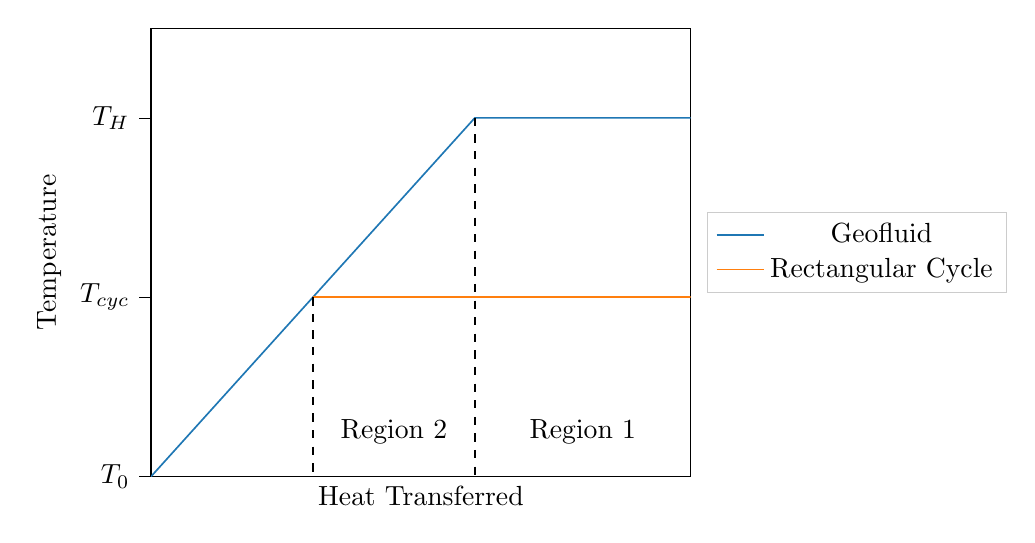
\begin{tikzpicture}

\definecolor{darkgray176}{RGB}{176,176,176}
\definecolor{darkorange25512714}{RGB}{255,127,14}
\definecolor{lightgray204}{RGB}{204,204,204}
\definecolor{steelblue31119180}{RGB}{31,119,180}

\begin{axis}[
legend style={
  fill opacity=0.8,
  draw opacity=1,
  text opacity=1,
  at={(1.03,0.5)},
  anchor=west,
  draw=lightgray204
},
tick align=outside,
tick pos=left,
x grid style={darkgray176},
xlabel={Heat Transferred},
xmin=0, xmax=10,
xtick style={color=black},
y grid style={darkgray176},
ylabel={Temperature},
ymin=0, ymax=10,
ytick style={color=black},
ytick={0,4,8},
yticklabels={
  \(\displaystyle {T_0}\),
  \(\displaystyle {T_{cyc}}\),
  \(\displaystyle {T_H}\)
},
xmajorticks=false
]
\addplot [semithick, steelblue31119180]
coordinates {
            (10, 8)
            (6, 8)
            (0, 0)
                };
\addlegendentry{Geofluid}
\addplot [semithick, darkorange25512714]
coordinates {
            (3, 4)
            (10, 4)
                };
\addlegendentry{Rectangular Cycle}
\addplot [semithick, black, dashed]
coordinates {
            (3, 4)
            (3, 0)
                };
\addplot [semithick, black, dashed]
coordinates {
            (6, 8)
            (6, 0)
                };

\node at (axis cs:8,0.5) [anchor=south] {Region 1};
\node at (axis cs:4.5,0.5) [anchor=south] {Region 2};
                
\end{axis}

\end{tikzpicture}

            \caption{Temperature-Duty diagram of the geofluid and the rectangular cyce.}
            \label{fig:TQ_Rect}
        \end{figure}
        
        To obtain an expression for the cycle efficiency that accounts for all irreversibilities associated with the heat transfer, the enthalpy and entropy balances of the overall system, as well as each of the regions identified must be considered. Where \(\Dot{m}_{H}\) is the mass rate of geofluid, \(h_{in}^{H}\) and \(h_{out}^{H}\) are the specific enthalpy of the geofluid at the inlet and outlet of the plant, \(s_{in}^{H}\) and \(s_{out}^{H}\) are the specific entropy of the geofluid at the inlet and outlet of the geofluid, \(\Dot{S}_{gen}^{tot}\) is the entropy generated, and \(T_0\) is the ambient temperature

        Overall:
        \begin{align}
             \Dot{m}_{H}(h_{in}^{H}-h_{out}^{H}) - \Dot{W}_{net} - \Dot{Q}_{out} = 0 \label{eq:rect_h_bal}
        \end{align}
        \begin{align}
             \Dot{m}_{H}(s_{in}^{H}-s_{out}^{H}) + \Dot{S}_{gen}^{tot} - \frac{\Dot{Q}_{out}}{T_0} = 0 \label{eq:rect_s_bal}
        \end{align}
        \begin{align}
             \frac{\Dot{Q}_{out}}{\Dot{Q}_{in}} = \frac{T_0 (s_{in}^{H}-s_{out}^{H}) + \frac{T_0\Dot{S}_{gen}^{tot}}{\Dot{m}_{H}}}{(h_{in}^{H}-h_{out}^{H})} \label{eq:rect_Qratio}
        \end{align}

        For Region 1:
        \begin{align}
             \Dot{m}_{H}(h_{in}^{H}-h_{sat}^{H}) = \Dot{m}_{F}(h_{out}^{F}-h_{*}^{F}) \label{eq:rect_h_bal_reg1}
        \end{align}
        \begin{align}
            \Dot{m}_{H}(s_{in}^{H}-s_{sat}^{H}) - \Dot{m}_{F}(s_{out}^{F}-s_{*}^{F}) + \Dot{S}_{gen}^{Region 1} = 0 \label{eq:rect_s_bal_reg1}
        \end{align}

        Where \(h_{sat}^{H}\) is the specific enthalpy of the geofluid at  saturation, \(s_{sat}^{H}\) is the specific entropy of the geofluid at saturation, \(\Dot{m}_{F}\) is the mass rate of working fluid, \(h_{out}^{F}\) and \(h_{*}^{F}\) are the specific enthalpy of the working fluid at the outlet of the heat exchanger and at the point where the geofluid reaches saturation, \(s_{out}^{F}\) and \(s_{*}^{F}\) are the specific entropy of the working fluid at the outlet of the heat exchanger and the point corresponding to saturation of the geofluid, and \(\Dot{S}_{gen}^{Region 1}\) is the entropy generated in Region 1.

        Combining Equations~\ref{eq:rect_s_bal_reg1} and \ref{eq:rect_h_bal_reg1}, recognising that evaporation/condensation of pure fluids occurs at constant temperature (at a given pressure), \(\Delta s_{fg}=\frac{\Delta h_{fg}}{T}\), we obtain an expression for the entropy generation associated with the heat transfer in Region 1, Equation~\ref{eq:rect_sgen_reg1}.

        \begin{align}
            \Dot{S}_{gen}^{Region 1} = \Dot{m}_{H}(h_{in}^{H}-h_{sat}^{H}) \left(\frac{1}{T_{cyc}} - \frac{1}{T_{H}}\right) \label{eq:rect_sgen_reg1}
        \end{align}

        A similar expression can be obtained for Region 2, Equation~\ref{eq:rect_sgen_reg2}.
        \begin{align}
             \Dot{m}_{H}(h_{sat}^{H}-h_{out}^{H}) = \Dot{m}_{F}(h_{*}^{F}-h_{in}^{F}) \label{eq:rect_h_bal_reg2}
        \end{align}
        \begin{align}
            \Dot{m}_{H}(s_{sat}^{H}-s_{out}^{H}) - \Dot{m}_{F}(s_{*}^{F}-s_{in}^{F}) + \Dot{S}_{gen}^{Region 2} = 0 \label{eq:rect_s_bal_reg2}
        \end{align}
        \begin{align}
            \Dot{S}_{gen}^{Region 2} = \Dot{m}_{H}(h_{sat}^{H}-h_{out}^{H})\frac{1}{T_{cyc}} - \Dot{m}_{H}(s_{sat}^{H}-s_{out}^{H}) \label{eq:rect_sgen_reg2}
        \end{align}

        Where \(h_{in}^{F}\) is the specific enthalpy of the working fluid at the inlet of the heat exchanger, \(s_{in}^{F}\) is the specific entropy of the working fluid at the inlet of the heat exchanger, and \(\Dot{S}_{gen}^{Region 2}\) is the entropy generated in Region 2.

        Combining Equations~\ref{eq:rect_sgen_reg1} and \ref{eq:rect_sgen_reg2}, yields an expression for the total entropy generation across the system, Equation~\ref{eq:rect_sgen_tot}, assuming that heat engine is mechanically ideal and does not introduce any irreversibilities.

        \begin{align}
            \frac{T_0\Dot{S}_{gen}^{tot}}{\Dot{m}_{H}} =\frac{T_0\Dot{S}_{gen}^{Region 1} + T_0\Dot{S}_{gen}^{Region 2}}{\Dot{m}_{H}}
        \end{align}
        % \begin{align}
        %     \frac{T_0\Dot{S}_{gen}^{tot}}{\Dot{m}_{H}} = (h_{in}^{H}-h_{sat}^{H}) \left(\frac{T_0}{T_{cyc}} - \frac{T_0}{T_{H}}\right) + (h_{sat}^{H}-h_{out}^{H})\frac{T_0}{T_{cyc}} - T_0(s_{sat}^{H}-s_{out}^{H})
        % \end{align}
        \begin{align}
            \frac{T_0\Dot{S}_{gen}^{tot}}{\Dot{m}_{H}} = (h_{in}^{H}-h_{out}^{H})\frac{T_0}{T_{cyc}} - (h_{in}^{H}-h_{sat}^{H})\frac{T_0}{T_{H}}  - T_0(s_{sat}^{H}-s_{out}^{H}) \label{eq:rect_sgen_tot}
        \end{align}

        Equation~\ref{eq:rect_sgen_tot} can then be substituted into Equation~\ref{eq:rect_Qratio}, which then simplifies to Equation~\ref{eq_rect_Qratio2} since then condensation of a pure fluid occurs at constant temperature and so \((s_{in}^{H}-s_{sat}^{H})=\frac{(h_{in}^{H}-h_{sat}^{H})}{T_H}\). Finally, the cycle efficiency is given by Equation~\ref{eq:rect_eff_cyc}. Where \(T_{cyc}\) is the cycle temperature.

        % \begin{align}
        %     \frac{\Dot{Q}_{out}}{\Dot{Q}_{in}} = \frac{(h_{in}^{H}-h_{out}^{H})\frac{T_0}{T_{cyc}} + T_0(s_{in}^{H}-s_{out}^{H}) - \frac{T_0}{T_{H}}(h_{in}^{H}-h_{sat}^{H}) - T_0(s_{sat}^{H}-s_{out}^{H})}{(h_{in}^{H}-h_{out}^{H})}
        % \end{align}
        \begin{align}
            \frac{\Dot{Q}_{out}}{\Dot{Q}_{in}} = \frac{T_0}{T_{cyc}} + \frac{(T_0(s_{in}^{H}-s_{sat}^{H}) - \frac{T_0}{T_{H}}(h_{in}^{H}-h_{sat}^{H})}{(h_{in}^{H}-h_{out}^{H})} 
        \end{align}

        % \begin{align}
        %     \frac{\Dot{Q}_{out}}{\Dot{Q}_{in}} = \frac{T_0}{T_{cyc}} + \frac{(\frac{T_0}{T_{H}}(h_{in}^{H}-h_{sat}^{H}) - \frac{T_0}{T_{H}}(h_{in}^{H}-h_{sat}^{H})}{(h_{in}^{H}-h_{out}^{H})} 
        % \end{align}
        \begin{align}
            \frac{\Dot{Q}_{out}}{\Dot{Q}_{in}} = \frac{T_0}{T_{cyc}} \label{eq_rect_Qratio2}
        \end{align}
        \begin{align}
            \eta_{cycle} = 1-\frac{\Dot{Q}_{out}}{\Dot{Q}_{in}} = 1-  \frac{T_0}{T_{cyc}} \label{eq:rect_eff_cyc}
        \end{align}

        The thermal recovery or thermal utilisation efficiency \(\eta_{recov}\) is then obtained via the ratio of the heat extracted from the heat source (by cooling it to a temperature \(T_{cyc}\)) to the maximum heat that could be extracted (by cooling the geofluid to a temperature of \(T_0\)), Equation~\ref{eq:rect_eff_recov}. Here \(\tau = T_H + \frac{x\Delta h_{fg}}{c_p}\), representing an \emph{effective} temperature of the geofluid at the inlet.

        \begin{align}
            \eta_{recov} =\frac{\Dot{Q}_{in}}{\Dot{Q}_{in}^{max}} = \frac{h_{in}^{H}-h_{out}^{H}}{h_{in}^{H}-h_{0}^{H}} = \frac{c_p (T_H - T_{cyc}) + x\Delta h_{fg}}{c_p (T_H - T_0) + x\Delta h_{fg}} 
        \end{align}
        % \begin{align}
        %     \eta_{recov} = \frac{T_H - T_{cyc} + \frac{x\Delta h_{fg}}{c_p}}{T_H - T_0 + \frac{x\Delta h_{fg}}{c_p}}
        % \end{align}
        \begin{align}
            \eta_{recov} = \frac{\tau - T_{cyc}}{\tau - T_0} \label{eq:rect_eff_recov}
        \end{align}

        The overall plant efficiency for the two-phase geofluid and the rectangular cycle, Equation~\ref{eq:rect_eff_plant}, is then obtained by combining Equations~\ref{eq:rect_eff_cyc} and \ref{eq:rect_eff_recov}. This expression is valid for any heat source that can be parameterised by Equation~\ref{eq:heat_content}.

        \begin{align}
            \eta_{plant} = \frac{\tau - T_{cyc}}{\tau - T_0} * \left(1-  \frac{T_0}{T_{cyc}}\right)\label{eq:rect_eff_plant}
        \end{align}
        
        % \begin{figure}[H]
        %     \centering
        %     % This file was created with tikzplotlib v0.10.1.
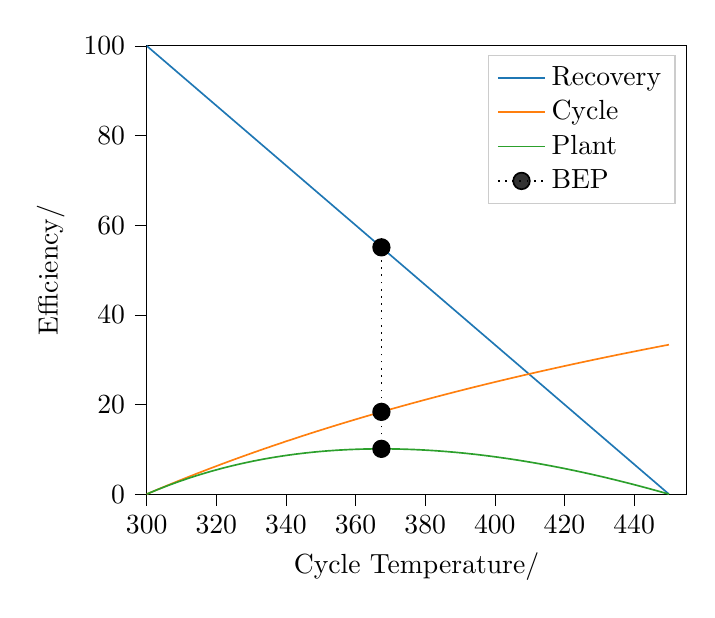
\begin{tikzpicture}

\definecolor{darkgray176}{RGB}{176,176,176}
\definecolor{darkorange25512714}{RGB}{255,127,14}
\definecolor{forestgreen4416044}{RGB}{44,160,44}
\definecolor{lightgray204}{RGB}{204,204,204}
\definecolor{steelblue31119180}{RGB}{31,119,180}

\begin{axis}[
legend cell align={left},
legend style={fill opacity=0.8, draw opacity=1, text opacity=1, draw=lightgray204},
tick align=outside,
tick pos=left,
x grid style={darkgray176},
xlabel={Cycle Temperature/\unit{\K}},
xmin=300, xmax=455,
xtick style={color=black},
y grid style={darkgray176},
ylabel={Efficiency/\unit{\percent}},
ymin=0, ymax=100,
ytick style={color=black}
]
\addplot [semithick, steelblue31119180]
table {%
300 100
303.061224489796 97.9591836734694
306.122448979592 95.9183673469388
309.183673469388 93.8775510204082
312.244897959184 91.8367346938776
315.30612244898 89.795918367347
318.367346938775 87.7551020408163
321.428571428571 85.7142857142857
324.489795918367 83.6734693877551
327.551020408163 81.6326530612245
330.612244897959 79.5918367346939
333.673469387755 77.5510204081633
336.734693877551 75.5102040816327
339.795918367347 73.469387755102
342.857142857143 71.4285714285714
345.918367346939 69.3877551020408
348.979591836735 67.3469387755102
352.040816326531 65.3061224489796
355.102040816327 63.265306122449
358.163265306122 61.2244897959184
361.224489795918 59.1836734693878
364.285714285714 57.1428571428572
367.34693877551 55.1020408163266
370.408163265306 53.0612244897959
373.469387755102 51.0204081632653
376.530612244898 48.9795918367347
379.591836734694 46.9387755102041
382.65306122449 44.8979591836735
385.714285714286 42.8571428571428
388.775510204082 40.8163265306123
391.836734693878 38.7755102040816
394.897959183673 36.734693877551
397.959183673469 34.6938775510204
401.020408163265 32.6530612244898
404.081632653061 30.6122448979592
407.142857142857 28.5714285714286
410.204081632653 26.5306122448979
413.265306122449 24.4897959183673
416.326530612245 22.4489795918367
419.387755102041 20.4081632653061
422.448979591837 18.3673469387755
425.510204081633 16.3265306122449
428.571428571429 14.2857142857143
431.632653061224 12.2448979591837
434.69387755102 10.2040816326531
437.755102040816 8.16326530612245
440.816326530612 6.12244897959185
443.877551020408 4.08163265306121
446.938775510204 2.0408163265306
450 0
};
\addlegendentry{Recovery}
\addplot [semithick, darkorange25512714]
table {%
300 0
303.061224489796 1.01010101010101
306.122448979592 1.99999999999999
309.183673469388 2.97029702970297
312.244897959184 3.92156862745098
315.30612244898 4.85436893203883
318.367346938775 5.76923076923076
321.428571428571 6.66666666666668
324.489795918367 7.54716981132075
327.551020408163 8.41121495327103
330.612244897959 9.25925925925926
333.673469387755 10.0917431192661
336.734693877551 10.9090909090909
339.795918367347 11.7117117117117
342.857142857143 12.5
345.918367346939 13.2743362831858
348.979591836735 14.0350877192982
352.040816326531 14.7826086956522
355.102040816327 15.5172413793103
358.163265306122 16.2393162393162
361.224489795918 16.9491525423729
364.285714285714 17.6470588235294
367.34693877551 18.3333333333333
370.408163265306 19.0082644628099
373.469387755102 19.672131147541
376.530612244898 20.3252032520325
379.591836734694 20.9677419354839
382.65306122449 21.6
385.714285714286 22.2222222222222
388.775510204082 22.8346456692913
391.836734693878 23.4375
394.897959183673 24.031007751938
397.959183673469 24.6153846153846
401.020408163265 25.1908396946565
404.081632653061 25.7575757575758
407.142857142857 26.3157894736842
410.204081632653 26.865671641791
413.265306122449 27.4074074074074
416.326530612245 27.9411764705882
419.387755102041 28.4671532846715
422.448979591837 28.9855072463768
425.510204081633 29.4964028776978
428.571428571429 30
431.632653061224 30.4964539007092
434.69387755102 30.9859154929577
437.755102040816 31.4685314685315
440.816326530612 31.9444444444444
443.877551020408 32.4137931034483
446.938775510204 32.8767123287671
450 33.3333333333333
};
\addlegendentry{Cycle}
\addplot [semithick, forestgreen4416044]
table {%
300 0
303.061224489796 0.989486703772414
306.122448979592 1.91836734693877
309.183673469388 2.78844210951708
312.244897959184 3.60144057623049
315.30612244898 4.35902516346344
318.367346938775 5.06279434850863
321.428571428571 5.71428571428572
324.489795918367 6.31497882171736
327.551020408163 6.86629792103758
330.612244897959 7.36961451247165
333.673469387755 7.82624976596143
336.734693877551 8.23747680890538
339.795918367347 8.60452289023718
342.857142857143 8.92857142857142
345.918367346939 9.21076395159835
348.979591836735 9.45220193340494
352.040816326531 9.65394853593611
355.102040816327 9.81703026038002
358.163265306122 9.94243851386709
361.224489795918 10.0311310965064
364.285714285714 10.0840336134454
367.34693877551 10.1020408163265
370.408163265306 10.0860178782257
373.469387755102 10.0368016058883
376.530612244898 9.95520159283226
379.591836734694 9.84200131665569
382.65306122449 9.69795918367347
385.714285714286 9.52380952380952
388.775510204082 9.32026353848626
391.836734693878 9.08801020408164
394.897959183673 8.82771713336497
397.959183673469 8.54003139717425
401.020408163265 8.22558030845926
404.081632653061 7.88497217068646
407.142857142857 7.51879699248121
410.204081632653 7.12762717027109
413.265306122449 6.71201814058957
416.326530612245 6.27250900360144
419.387755102041 5.80962311932072
422.448979591837 5.32386867790594
425.510204081633 4.81573924533842
428.571428571429 4.28571428571429
431.632653061224 3.73425966131134
434.69387755102 3.16182811152631
437.755102040816 2.56885971171686
440.816326530612 1.95578231292517
443.877551020408 1.32301196340605
446.938775510204 0.670953312831979
450 0
};
\addlegendentry{Plant}
\addplot [semithick, black, dotted, mark=*, mark size=3, mark options={solid}]
table {%
367.423461417477 10.1020514433644
367.423461417477 18.3503419072274
367.423461417477 55.0510257216822
};
\addlegendentry{BEP}
\end{axis}

\end{tikzpicture}

        %     \caption[The thermal recovery, cycle and plant efficiency for a Rectangular cycle and a sensible heat dominated heat-source.]{The thermal recovery, cycle and plant efficiency as a function of the maximum cycle temperature for a Rectangular cycle and a heat source characterised by a \(C_p\) of \qty{4}{\kilo\joule\per\kg\per\K}, a latent heat of \(x\Delta H_{fh}\) of \qty{0}{\kilo\joule\per\kg}, an inlet temperature of \qty{450}{\K} and an ambient temperature of \qty{300}{\K}. The black points indicate the best efficiency point}
        %     \label{fig:litrev_SaturatedSource_Rectangular}
        % \end{figure}

        The optimum cycle temperature \(T_{cyc}^{opt}\) can then by determined by finding the cycle temperature \(T_{cyc}\), for which \(\frac{d\eta_{plant}}{dT_{cyc}}=0\), Equations~\ref{eq:rect_deff_plantdTcyc} and \ref{eq:rect_Tcyc_opt}. Equation~\ref{eq:rect_Tcyc_opt} is valid up to \(\frac{x\Delta h_{fg}}{c_p} = T_H\left(\frac{T_H}{T_0}-1\right)\), above which, the optimum cycle temperature is equal to the temperature of the heat source \(T_H\).

        \begin{align}
            \frac{d\eta_{plant}}{dT_{cyc}} = -\frac{1}{\tau - T_0} + \frac{1}{\tau T_0} \frac{1}{T_{cyc}^2}\label{eq:rect_deff_plantdTcyc}
        \end{align}

        \begin{align}
            T_{cyc}^{opt} = \sqrt{\tau T_0}=\sqrt{T_0 * \left(T_H + \frac{x\Delta h_{fg}}{c_p}\right)} \label{eq:rect_Tcyc_opt}
        \end{align}

        \begin{figure}[H]
            \centering
            % This file was created with tikzplotlib v0.10.1.
\begin{tikzpicture}

\definecolor{crimson2143940}{RGB}{214,39,40}
\definecolor{darkgray176}{RGB}{176,176,176}
\definecolor{darkorange25512714}{RGB}{255,127,14}
\definecolor{forestgreen4416044}{RGB}{44,160,44}
\definecolor{lightgray204}{RGB}{204,204,204}
\definecolor{mediumpurple148103189}{RGB}{148,103,189}
\definecolor{steelblue31119180}{RGB}{31,119,180}

\begin{axis}[
legend cell align={left},
legend style={
  fill opacity=0.8,
  draw opacity=1,
  text opacity=1,
  at={(1.03,0.5)},
  anchor=west,
  draw=lightgray204
},
tick align=outside,
tick pos=left,
x grid style={darkgray176},
xlabel={Cycle Temperature/\unit{\K}},
xmin=300, xmax=455,
xtick style={color=black},
y grid style={darkgray176},
ylabel={Efficiency/\unit{\percent}},
ymin=0, ymax=40,
ytick style={color=black}
]
\addplot [semithick, steelblue31119180]
table {%
300 0
303.061224489796 0.989486703772414
306.122448979592 1.91836734693877
309.183673469388 2.78844210951708
312.244897959184 3.60144057623049
315.30612244898 4.35902516346344
318.367346938775 5.06279434850863
321.428571428571 5.71428571428572
324.489795918367 6.31497882171736
327.551020408163 6.86629792103758
330.612244897959 7.36961451247165
333.673469387755 7.82624976596143
336.734693877551 8.23747680890538
339.795918367347 8.60452289023718
342.857142857143 8.92857142857142
345.918367346939 9.21076395159835
348.979591836735 9.45220193340494
352.040816326531 9.65394853593611
355.102040816327 9.81703026038002
358.163265306122 9.94243851386709
361.224489795918 10.0311310965064
364.285714285714 10.0840336134454
367.34693877551 10.1020408163265
370.408163265306 10.0860178782257
373.469387755102 10.0368016058883
376.530612244898 9.95520159283226
379.591836734694 9.84200131665569
382.65306122449 9.69795918367347
385.714285714286 9.52380952380952
388.775510204082 9.32026353848626
391.836734693878 9.08801020408164
394.897959183673 8.82771713336497
397.959183673469 8.54003139717425
401.020408163265 8.22558030845926
404.081632653061 7.88497217068646
407.142857142857 7.51879699248121
410.204081632653 7.12762717027109
413.265306122449 6.71201814058957
416.326530612245 6.27250900360144
419.387755102041 5.80962311932072
422.448979591837 5.32386867790594
425.510204081633 4.81573924533842
428.571428571429 4.28571428571429
431.632653061224 3.73425966131134
434.69387755102 3.16182811152631
437.755102040816 2.56885971171686
440.816326530612 1.95578231292517
443.877551020408 1.32301196340605
446.938775510204 0.670953312831979
450 0
};
\addlegendentry{\(\frac{x\Delta h_{fg}}{c_p}=\)\qty{0}{\kilo\joule\per\kg}}
\addplot [semithick, darkorange25512714]
table {%
300 0
303.061224489796 0.998856843012683
306.122448979592 1.95547309833023
309.183673469388 2.8711034368743
312.244897959184 3.74695332678526
315.30612244898 4.5841814219068
318.367346938775 5.38390181247323
321.428571428571 6.14718614718616
324.489795918367 6.87506563517345
327.551020408163 7.56853293568915
330.612244897959 8.22854394282965
333.673469387755 8.85601947200899
336.734693877551 9.45184685444426
339.795918367347 10.0168814454529
342.857142857143 10.551948051948
345.918367346939 11.0578422841381
348.979591836735 11.5353318360837
352.040816326531 11.9851576994434
355.102040816327 12.4080353144393
358.163265306122 12.8046556617985
361.224489795918 13.175686299173
364.285714285714 13.5217723453018
367.34693877551 13.843537414966
370.408163265306 14.1415845075821
373.469387755102 14.416496852094
376.530612244898 14.6688387106506
379.591836734694 14.8991561433958
382.65306122449 15.1079777365492
385.714285714286 15.2958152958153
388.775510204082 15.463164507034
391.836734693878 15.6105055658627
394.897959183673 15.7383037781709
397.959183673469 15.8470101327244
401.020408163265 15.9370618476398
404.081632653061 16.0088828919998
407.142857142857 16.0628844839371
410.204081632653 16.0994655664165
413.265306122449 16.1190132618704
416.326530612245 16.1219033067773
419.387755102041 16.1085004672075
422.448979591837 16.0791589363018
425.510204081633 16.0342227145927
428.571428571429 15.974025974026
431.632653061224 15.8988934064922
434.69387755102 15.8091405576315
437.755102040816 15.7050741466326
440.816326530612 15.5869923727067
443.877551020408 15.4551852088798
446.938775510204 15.3099346837116
450 15.1515151515152
};
\addlegendentry{\(\frac{x\Delta h_{fg}}{c_p}=\)\qty{125}{\kilo\joule\per\kg}}
\addplot [semithick, forestgreen4416044]
table {%
300 0
303.061224489796 1.00237064522778
306.122448979592 1.96938775510203
309.183673469388 2.90210143463326
312.244897959184 3.80152060824329
315.30612244898 4.66861501882306
318.367346938775 5.50431711145996
321.428571428571 6.30952380952382
324.489795918367 7.08509819021948
327.551020408163 7.83187106618348
330.612244897959 8.55064247921391
333.673469387755 9.24218311177683
336.734693877551 9.90723562152134
339.795918367347 10.5465159036588
342.857142857143 11.1607142857143
345.918367346939 11.7504966588405
348.979591836735 12.3165055495883
352.040816326531 12.8593611357586
355.102040816327 13.3796622097115
358.163265306122 13.8779870922728
361.224489795918 14.3548945001729
364.285714285714 14.8109243697479
367.34693877551 15.2465986394558
370.408163265306 15.6624219935908
373.469387755102 16.0588825694212
376.530612244898 16.4364526298324
379.591836734694 16.7955892034233
382.65306122449 17.1367346938775
385.714285714286 17.4603174603175
388.775510204082 17.7667523702394
391.836734693878 18.0564413265306
394.897959183673 18.3297737699731
397.959183673469 18.5871271585557
401.020408163265 18.8288674248325
404.081632653061 19.0553494124923
407.142857142857 19.2669172932331
410.204081632653 19.4639049649711
413.265306122449 19.6466364323507
416.326530612245 19.8154261704682
419.387755102041 19.970579472665
422.448979591837 20.1123927832002
425.510204081633 20.2411540155631
428.571428571429 20.3571428571429
431.632653061224 20.460631060935
434.69387755102 20.551882724921
437.755102040816 20.631154559726
440.816326530612 20.6986961451247
443.877551020408 20.7547501759324
446.938775510204 20.7995526977914
450 20.8333333333333
};
\addlegendentry{\(\frac{x\Delta h_{fg}}{c_p}=\)\qty{250}{\kilo\joule\per\kg}}
\addplot [semithick, crimson2143940]
table {%
300 0
303.061224489796 1.00534386248672
306.122448979592 1.9811616954474
309.183673469388 2.92833050966007
312.244897959184 3.84769292332317
315.30612244898 4.74005883159836
318.367346938775 5.60620697983335
321.428571428571 6.44688644688646
324.489795918367 7.2628180444892
327.551020408163 8.05469563814023
330.612244897959 8.82318739461596
333.673469387755 9.56893696081115
336.734693877551 10.2925645782789
339.795918367347 10.9946681375253
342.857142857143 11.6758241758242
345.918367346939 12.3365888220503
348.979591836735 12.9774986917844
352.040816326531 13.5990717357177
355.102040816327 14.2018080441726
358.163265306122 14.7861906103664
361.224489795918 15.3526860548652
364.285714285714 15.90174531351
367.34693877551 16.4338042909471
370.408163265306 16.949284481752
373.469387755102 17.4485935610057
376.530612244898 17.9321259460632
379.591836734694 18.4002633311389
382.65306122449 18.8533751962323
385.714285714286 19.2918192918193
388.775510204082 19.715942100644
391.836734693878 20.126079277865
394.897959183673 20.5225560707288
397.959183673469 20.9056877188745
401.020408163265 21.2757798363033
404.081632653061 21.6331287759859
407.142857142857 21.978021978022
410.204081632653 22.3107383022095
413.265306122449 22.6315483458341
416.326530612245 22.9407147474374
419.387755102041 23.2384924772829
422.448979591837 23.5251291151912
425.510204081633 23.8008651163841
428.571428571429 24.0659340659341
431.632653061224 24.3205629223866
434.69387755102 24.5649722510889
437.755102040816 24.7993764477281
440.816326530612 25.0239839525554
443.877551020408 25.2389974557462
446.938775510204 25.4446140943205
450 25.6410256410256
};
\addlegendentry{\(\frac{x\Delta h_{fg}}{c_p}=\)\qty{500}{\kilo\joule\per\kg}}
\addplot [semithick, mediumpurple148103189]
table {%
300 0
303.061224489796 1.00741218753641
306.122448979592 1.98935226264418
309.183673469388 2.9465768227222
312.244897959184 3.87981279468309
315.30612244898 4.78975887526813
318.367346938775 5.677086888267
321.428571428571 6.5424430641822
324.489795918367 7.38644924745944
327.551020408163 8.20970403602319
330.612244897959 9.01278385750435
333.673469387755 9.79624398622633
336.734693877551 10.5606195047189
339.795918367347 11.3064262132585
342.857142857143 12.0341614906832
345.918367346939 12.7443051095005
348.979591836735 13.4373200080948
352.040816326531 14.1136530226457
355.102040816327 14.773735581189
358.163265306122 15.4179843620838
361.224489795918 16.046801918999
364.285714285714 16.660577274388
367.34693877551 17.259686483289
370.408163265306 17.8444931691685
373.469387755102 18.4153490334124
376.530612244898 18.9725943399629
379.591836734694 19.5165583765063
382.65306122449 20.0475598935226
385.714285714286 20.5659075224293
388.775510204082 21.0719001739689
391.836734693878 21.5658274179237
394.897959183673 22.0479698451676
397.959183673469 22.5185994130094
401.020408163265 22.9779797747177
404.081632653061 23.4263665940685
407.142857142857 23.8640078457012
410.204081632653 24.2911441020276
413.265306122449 24.7080088073877
416.326530612245 25.1148285401117
419.387755102041 25.511823263104
422.448979591837 25.8992065635328
425.510204081633 26.2771858821727
428.571428571429 26.6459627329192
431.632653061224 27.0057329129617
434.69387755102 27.3566867040754
437.755102040816 27.6990090654687
440.816326530612 28.0328798185941
443.877551020408 28.3584738243123
446.938775510204 28.6759611527756
450 28.9855072463768
};
\addlegendentry{\(\frac{x\Delta h_{fg}}{c_p}=\)\qty{1000}{\kilo\joule\per\kg}}
\addplot [semithick, black, dashed]
table {%
300 0
303.061224489796 1.01010101010101
306.122448979592 1.99999999999999
309.183673469388 2.97029702970297
312.244897959184 3.92156862745098
315.30612244898 4.85436893203883
318.367346938775 5.76923076923076
321.428571428571 6.66666666666668
324.489795918367 7.54716981132075
327.551020408163 8.41121495327103
330.612244897959 9.25925925925926
333.673469387755 10.0917431192661
336.734693877551 10.9090909090909
339.795918367347 11.7117117117117
342.857142857143 12.5
345.918367346939 13.2743362831858
348.979591836735 14.0350877192982
352.040816326531 14.7826086956522
355.102040816327 15.5172413793103
358.163265306122 16.2393162393162
361.224489795918 16.9491525423729
364.285714285714 17.6470588235294
367.34693877551 18.3333333333333
370.408163265306 19.0082644628099
373.469387755102 19.672131147541
376.530612244898 20.3252032520325
379.591836734694 20.9677419354839
382.65306122449 21.6
385.714285714286 22.2222222222222
388.775510204082 22.8346456692913
391.836734693878 23.4375
394.897959183673 24.031007751938
397.959183673469 24.6153846153846
401.020408163265 25.1908396946565
404.081632653061 25.7575757575758
407.142857142857 26.3157894736842
410.204081632653 26.865671641791
413.265306122449 27.4074074074074
416.326530612245 27.9411764705882
419.387755102041 28.4671532846715
422.448979591837 28.9855072463768
425.510204081633 29.4964028776978
428.571428571429 30
431.632653061224 30.4964539007092
434.69387755102 30.9859154929577
437.755102040816 31.4685314685315
440.816326530612 31.9444444444444
443.877551020408 32.4137931034483
446.938775510204 32.8767123287671
450 33.3333333333333
};
\addlegendentry{\(\frac{x\Delta h_{fg}}{c_p}=\infty\) \unit{\kilo\joule\per\kg}}
\addplot [semithick, black, dotted, mark=*, mark size=3, mark options={solid}]
table {%
367.423461417477 10.1020514433644
415.331193145904 16.1227686211609
450 20.8333333333333
450 25.6410256410256
450 28.9855072463768
450 33.3333333333333
};
\addlegendentry{BEP}
\end{axis}

\end{tikzpicture}

            \caption[The overall plant efficiency for different latent heats as a function of maximum cycle temperature.]{The overall plant efficiency as a function of the cycle temperature for a Rectangular cycle and a heat source characterised by a \(c_p\) of \qty{4}{\kilo\joule\per\kg\per\K}, a latent heat \(x\Delta H_{fh}\) of \qty{0}{\kilo\joule\per\kg}, an inlet temperature of \qty{450}{\K} and an ambient temperature of \qty{300}{\K}}
            \label{fig:litrev_GenericSource_Carnot}
        \end{figure}

        \subsubsection{Triangular Cycle}

        Assuming the specific heat capacity of the working fluid is constant over the range of temperatures of interest, Figure~\ref{fig:TQ_Tri} shows the temperature duty diagram for the geofluid and the triangular cycle. Similarly to the rectangular cycle two distinct regions emerge, Region 1 where the latent heat of condensation of the geofluid provides sensible heat to the working fluid, and Region 2 where the sensible heat of the geofluid provides sensible heat to the working fluid.

        \begin{figure}[H]
            \centering
            % This file was created with tikzplotlib v0.10.1.
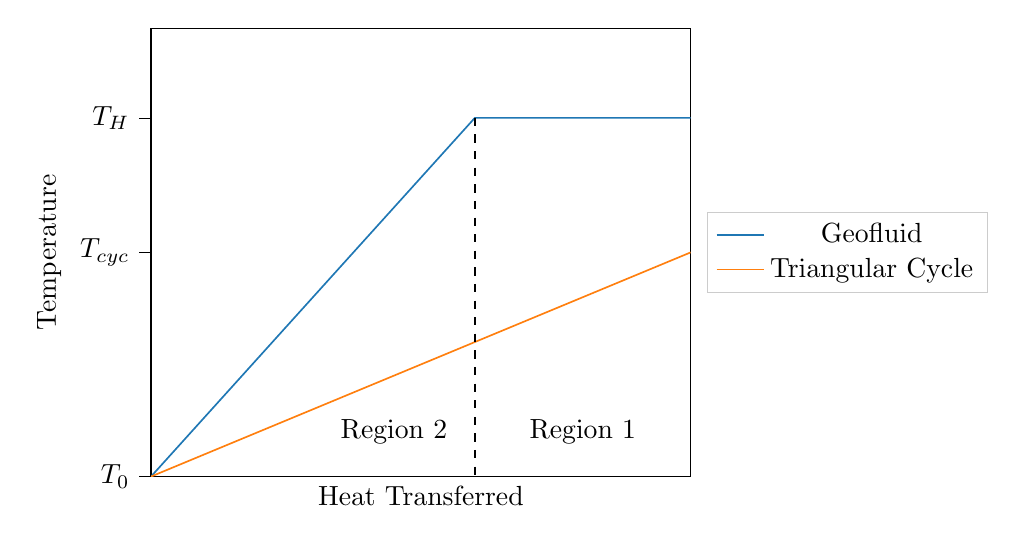
\begin{tikzpicture}

\definecolor{darkgray176}{RGB}{176,176,176}
\definecolor{darkorange25512714}{RGB}{255,127,14}
\definecolor{lightgray204}{RGB}{204,204,204}
\definecolor{steelblue31119180}{RGB}{31,119,180}

\begin{axis}[
legend style={
  fill opacity=0.8,
  draw opacity=1,
  text opacity=1,
  at={(1.03,0.5)},
  anchor=west,
  draw=lightgray204
},
tick align=outside,
tick pos=left,
x grid style={darkgray176},
xlabel={Heat Transferred},
xmin=0, xmax=10,
xtick style={color=black},
y grid style={darkgray176},
ylabel={Temperature},
ymin=0, ymax=10,
ytick style={color=black},
ytick={0, 5, 8},
yticklabels={
  \(\displaystyle {T_0}\),
  \(\displaystyle {T_{cyc}}\),
  \(\displaystyle {T_H}\)
},
xmajorticks=false
]
\addplot [semithick, steelblue31119180]
coordinates {
            (10, 8)
            (6, 8)
            (0, 0)
                };
\addlegendentry{Geofluid}
\addplot [semithick, darkorange25512714]
coordinates {
            (0, 0)
            (10, 5)
                };
\addlegendentry{Triangular Cycle}
% \addplot [semithick, black, dashed]
% coordinates {
%             (3.75, 5)
%             (3.75, 0)
%                 };
\addplot [semithick, black, dashed]
coordinates {
            (6, 8)
            (6, 0)
                };

\node at (axis cs:8,0.5) [anchor=south] {Region 1};
\node at (axis cs:4.5,0.5) [anchor=south] {Region 2};
                
\end{axis}

\end{tikzpicture}

            \caption{Temperature-Duty diagram of the geofluid and the triangular cycle.}
            \label{fig:TQ_Tri}
        \end{figure}

        To obtain an expression for the cycle efficiency that accounts for all irreversibilities associated with the heat transfer, the enthalpy and entropy balances of the overall system, as well as each of the regions identified must be considered. The nomenclature is used is consistent with that used in the previous chapter.

        Overall:
        \begin{align}
             \Dot{m}_{H}(h_{in}^{H}-h_{out}^{H}) - \Dot{W}_{net} - \Dot{Q}_{out} = 0\label{eq:tri_h_bal}
        \end{align}
        \begin{align}
             \Dot{m}_{H}(s_{in}^{H}-s_{out}^{H}) + \Dot{S}_{gen}^{tot} - \frac{\Dot{Q}_{out}}{T_0} = 0 \label{eq:tri_s_bal}
        \end{align}

        \begin{align}
             \frac{\Dot{Q}_{out}}{\Dot{Q}_{in}} = \frac{T_0 (s_{in}^{H}-s_{out}^{H}) + \frac{T_0\Dot{S}_{gen}^{tot}}{\Dot{m}_{H}}}{(h_{in}^{H}-h_{out}^{H})} \label{eq:tri_Qratio}
        \end{align}

        For Region 1:
        \begin{align}
             \Dot{m}_{H}(h_{in}^{H}-h_{sat}^{H}) = \Dot{m}_{F}(h_{out}^{F}-h_{*}^{F}) \label{eq:tri_h_bal_reg1}
        \end{align}
        \begin{align}
            \Dot{m}_{H}(s_{in}^{H}-s_{sat}^{H}) - \Dot{m}_{F}(s_{out}^{F}-s_{*}^{F}) + \Dot{S}_{gen}^{Region 1} = 0 \label{eq:tri_s_bal_reg1}
        \end{align}

       Since condensation of of pure fluids occurs at constant temperature (at a given pressure), \(\Delta s_{fg}=\frac{\Delta h_{fg}}{T}\), this yields Equation~\ref{eq:tri_sgen_reg1} as an expression for the entropy generation associated with the heat transfer in Region 1.

        \begin{align}
            \Dot{S}_{gen}^{Region 1} = \Dot{m}_{F}(s_{out}^{F}-s_{*}^{F}) - \Dot{m}_{H} \frac{(h_{in}^{H}-h_{sat}^{H})}{T_H}\label{eq:tri_sgen_reg1}
        \end{align}

        A similar expression can be obtained for Region 2, Equation~\ref{eq:tri_sgen_reg2}.
        \begin{align}
             \Dot{m}_{H}(h_{sat}^{H}-h_{out}^{H}) = \Dot{m}_{F}(h_{*}^{F}-h_{in}^{F}) \label{eq:tri_h_bal_reg2}
        \end{align}
        \begin{align}
            \Dot{m}_{H}(s_{sat}^{H}-s_{out}^{H}) - \Dot{m}_{F}(s_{*}^{F}-s_{in}^{F}) + \Dot{S}_{gen}^{Region 2} = 0 \label{eq:tri_s_bal_reg2}
        \end{align}
        \begin{align}
            \Dot{S}_{gen}^{Region 2} = \Dot{m}_{F}(s_{*}^{F}-s_{in}^{F}) - \Dot{m}_{H}(s_{sat}^{H}-s_{out}^{H})  \label{eq:tri_sgen_reg2}
        \end{align}

        Combining Equations~\ref{eq:tri_sgen_reg1} and \ref{eq:tri_sgen_reg2}, yields an expression for the total entropy generation across the system, Equation~\ref{eq:rect_sgen_tot}, assuming that heat engine is mechanically ideal and does not introduce any irreversibilities.

        \begin{align}
            \Dot{S}_{gen}^{tot} = \Dot{m}_{F}(s_{out}^{F}-s_{*}^{F} + s_{*}^{F}-s_{in}^{F}) - \Dot{m}_{H} \frac{(h_{in}^{H}-h_{sat}^{H})}{T_H} - \Dot{m}_{H}(s_{sat}^{H}-s_{out}^{H})
        \end{align}
        \begin{align}
            \frac{T_0\Dot{S}_{gen}^{tot}}{\Dot{m}_{H}} = \frac{\Dot{m}_{F}}{\Dot{m}_{H}}T_0(s_{out}^{F}-s_{in}^{F}) - (h_{in}^{H}-h_{sat}^{H})\frac{T_0}{T_H} - T_0(s_{sat}^{H}-s_{out}^{H}) \label{eq:tri_sgen_tot}
        \end{align}

        Substituting Equation~\ref{eq:tri_sgen_tot} into Equation~\ref{eq:tri_Qratio}, yields an expression for the ration of the heat transferred out of and into the system. Since the condensation of the geofluid occurs at constant temperature \((s_{in}^{H}-s_{sat}^{H})=\frac{(h_{in}^{H}-h_{sat}^{H})}{T_H}\), this then simplifies to Equation~\ref{eq:tri_Qratio2}.
        \begin{align}
            \frac{\Dot{Q}_{out}}{\Dot{Q}_{in}} = \frac{T_0(s_{in}^{H}-s_{out}^{H} - s_{sat}^{H}+s_{out}^{H}) - \frac{T_0}{T_{H}}(h_{in}^{H}-h_{sat}^{H}) + \frac{\Dot{m}_{F}}{\Dot{m}_{H}}T_0(s_{out}^{F}-s_{in}^{F})}{(h_{in}^{H}-h_{out}^{H})}
        \end{align}
        % \begin{align}
        %     \frac{\Dot{Q}_{out}}{\Dot{Q}_{in}} = \frac{T_0(s_{in}^{H} - s_{sat}^{H}) - \frac{T_0}{T_{H}}(h_{in}^{H}-h_{sat}^{H}) + \frac{\Dot{m}_{F}}{\Dot{m}_{H}}T_0(s_{out}^{F}-s_{in}^{F})}{(h_{in}^{H}-h_{out}^{H})}
        % \end{align}
        \begin{align}
            \frac{\Dot{Q}_{out}}{\Dot{Q}_{in}} = \frac{\Dot{m}_{F}}{\Dot{m}_{H}}\frac{T_0(s_{out}^{F}-s_{in}^{F})}{(h_{in}^{H}-h_{out}^{H})} \label{eq:tri_Qratio2}
        \end{align}
        
        As the heat released by the geofluid is absorbed by the working fluid, the mass rate ratio \(\frac{\Dot{m}_{F}}{\Dot{m}_{H}}\) is given by Equation~\ref{eq:tri_Mratio}. Moreover, assuming the working fluid has a constant specific heat capacity over the temperatures of interest, the difference in enthalpy and entropy are given by Equations~\ref{eq:tri_deltah} and \ref{eq:tri_deltas} respectively. Combined they yield Equation~\ref{eq:tri_Qratio3}, and in turn the cycle efficiency, Equation~\ref{eq:tri_eff_cyc}

        \begin{align}
            \frac{\Dot{m}_{F}}{\Dot{m}_{H}}=\frac{(h_{in}^{H}-h_{out}^{H})}{(h_{out}^{F}-h_{in}^{F})} \label{eq:tri_Mratio}
        \end{align}
        \begin{align}
            h_{out}^{F}-h_{in}^{F}=c_p^F(T_{cyc}-T_0) \label{eq:tri_deltah}
        \end{align}
        \begin{align}
            s_{out}^{F}-s_{in}^{F}=c_p^F \ln \frac{T_{cyc}}{T_0} \label{eq:tri_deltas}
        \end{align}        
        \begin{align}
            \frac{\Dot{Q}_{out}}{\Dot{Q}_{in}} = T_0\frac{c_p^F \ln \frac{T_{cyc}}{T_0}}{c_p^F(T_{cyc}-T_0)}=\frac{T_0}{\frac{T_{cyc}-T_0}{\ln \frac{T_{cyc}}{T_0}}}=\frac{T_0}{T_{cyc}^{LM}} \label{eq:tri_Qratio3}
        \end{align}
        \begin{align}
            \eta_{cycle} = 1-\frac{\Dot{Q}_{out}}{\Dot{Q}_{in}} = 1-  \frac{T_0}{T_{cyc}^{LM}} \label{eq:tri_eff_cyc}
        \end{align}

        With regards to the thermal recovery (or utilisation) efficiency, unlike the rectangular cycle, the heat extracted from the heat source is not limited by the existence of a pinch point - assuming a minimum approach temperature difference of zero as a simplification. As such, the heat extracted from the geofluid is not a function of the cycle temperature, and the thermal recovery efficiency \(\eta_{recov}\) is \num{1}, and the overall plant efficiency \(\eta_{plant}\) is only dependent on the cycle efficiency \(\eta_{cycle}\) of the triangular cycle. 

        In terms of the optimum cycle temperature, this is equal to the source temperature, as this minimises the magnitude of \(\frac{\Dot{Q}_{out}}{\Dot{Q}_{in}}\).

        \begin{align}
            T_{cyc}^{opt} = T_H \label{eq:tri_T_cyc_opt}
        \end{align}

        \subsubsection{Direct Comparison}

         Comparing the overall plant efficiency of the Triangular and Rectangular cycle plants for different values of \(\frac{x\Delta h_{fg}}{c_p}\), Triangular cycle can be seen to provide better overall plant efficiencies than the Carnot cycle plant for \(\frac{x\Delta h_{fg}}{c_p}\) as high as \qty{198}{K}, Figure~\ref{fig:litrev_GenericSource_Carnot_vs_Triangular}. The critical ratio of latent heat to the specific heat capacity is given by Equation~\ref{eq:carnot_triangular_crit_point}. For combinations of latent heat and specific heat capacity in excess of this critical point, the Rectangular cycle outperforms the Triangular cycle.

         \begin{align}
           \frac{x\Delta H_{fg}}{C_p}_{crit} = \frac{T_H(T_{LM}-T_0)}{T_{LM}-T_H\left(\frac{T_{LM}-T_0}{T_H-T0}\right)}  \label{eq:carnot_triangular_crit_point}
        \end{align}

        \begin{figure}[H]
            \centering
            % This file was created with tikzplotlib v0.10.1.
\begin{tikzpicture}

\definecolor{crimson2143940}{RGB}{214,39,40}
\definecolor{darkgray176}{RGB}{176,176,176}
\definecolor{darkorange25512714}{RGB}{255,127,14}
\definecolor{forestgreen4416044}{RGB}{44,160,44}
\definecolor{lightgray204}{RGB}{204,204,204}
\definecolor{mediumpurple148103189}{RGB}{148,103,189}
\definecolor{sienna1408675}{RGB}{140,86,75}
\definecolor{steelblue31119180}{RGB}{31,119,180}

\begin{axis}[
legend cell align={left},
legend style={
  fill opacity=0.8,
  draw opacity=1,
  text opacity=1,
  at={(1.03,0.5)},
  anchor=west,
  draw=lightgray204
},
tick align=outside,
tick pos=left,
x grid style={darkgray176},
xlabel={Cycle Temperature/\unit{\K}},
xmin=300, xmax=455,
xtick style={color=black},
y grid style={darkgray176},
ylabel={Plant Efficiency/\unit{\percent}},
ymin=0, ymax=40,
ytick style={color=black}
]
\addplot [semithick, steelblue31119180]
table {%
300 0
303.061224489796 0.989486703772414
306.122448979592 1.91836734693877
309.183673469388 2.78844210951708
312.244897959184 3.60144057623049
315.30612244898 4.35902516346344
318.367346938775 5.06279434850863
321.428571428571 5.71428571428572
324.489795918367 6.31497882171736
327.551020408163 6.86629792103758
330.612244897959 7.36961451247165
333.673469387755 7.82624976596143
336.734693877551 8.23747680890538
339.795918367347 8.60452289023718
342.857142857143 8.92857142857142
345.918367346939 9.21076395159835
348.979591836735 9.45220193340494
352.040816326531 9.65394853593611
355.102040816327 9.81703026038002
358.163265306122 9.94243851386709
361.224489795918 10.0311310965064
364.285714285714 10.0840336134454
367.34693877551 10.1020408163265
370.408163265306 10.0860178782257
373.469387755102 10.0368016058883
376.530612244898 9.95520159283226
379.591836734694 9.84200131665569
382.65306122449 9.69795918367347
385.714285714286 9.52380952380952
388.775510204082 9.32026353848626
391.836734693878 9.08801020408164
394.897959183673 8.82771713336497
397.959183673469 8.54003139717425
401.020408163265 8.22558030845926
404.081632653061 7.88497217068646
407.142857142857 7.51879699248121
410.204081632653 7.12762717027109
413.265306122449 6.71201814058957
416.326530612245 6.27250900360144
419.387755102041 5.80962311932072
422.448979591837 5.32386867790594
425.510204081633 4.81573924533842
428.571428571429 4.28571428571429
431.632653061224 3.73425966131134
434.69387755102 3.16182811152631
437.755102040816 2.56885971171686
440.816326530612 1.95578231292517
443.877551020408 1.32301196340605
446.938775510204 0.670953312831979
450 0
};
\addlegendentry{\(\frac{x\Delta H_{fg}}{c_p}=\)\qty{0}{\kilo\joule\per\kg}}
\addplot [semithick, darkorange25512714]
table {%
300 0
303.061224489796 0.995549735045529
306.122448979592 1.9423769507803
309.183673469388 2.84192885074822
312.244897959184 3.69559588541299
315.30612244898 4.50471450716209
318.367346938775 5.27056976636808
321.428571428571 5.99439775910365
324.489795918367 6.6773879363066
327.551020408163 7.32068528345918
330.612244897959 7.92539237917389
333.673469387755 8.4925713404628
336.734693877551 9.02324566190113
339.795918367347 9.51840195537675
342.857142857143 9.97899159663865
345.918367346939 10.4059322844182
348.979591836735 10.8001095174912
352.040816326531 11.1623779946761
355.102040816327 11.4935629424183
358.163265306122 11.7944613742933
361.224489795918 12.0658432864671
364.285714285714 12.3084527928819
367.34693877551 12.5230092036815
370.408163265306 12.7102080501622
373.469387755102 12.8707220593155
376.530612244898 13.0052020808323
379.591836734694 13.1142779692522
382.65306122449 13.1985594237695
385.714285714286 13.2586367880486
388.775510204082 13.2950818122525
391.836734693878 13.3084483793517
394.897959183673 13.2992731976512
397.959183673469 13.2680764613538
401.020408163265 13.2153624808702
404.081632653061 13.1416202844774
407.142857142857 13.047324192835
410.204081632653 12.932934367777
413.265306122449 12.7988973367125
416.326530612245 12.6456464938917
419.387755102041 12.473602579718
422.448979591837 12.2831741392209
425.510204081633 12.0747579607383
428.571428571429 11.8487394957983
431.632653061224 11.6054932611342
434.69387755102 11.345383223712
437.755102040816 11.0687631696035
440.816326530612 10.7759770574897
443.877551020408 10.4673593575361
446.938775510204 10.1432353763423
450 9.80392156862745
};
\addlegendentry{\(\frac{x\Delta H_{fg}}{c_p}=\)\qty{62.5}{\kilo\joule\per\kg}}
\addplot [semithick, forestgreen4416044]
table {%
300 0
303.061224489796 0.998856843012683
306.122448979592 1.95547309833023
309.183673469388 2.8711034368743
312.244897959184 3.74695332678526
315.30612244898 4.5841814219068
318.367346938775 5.38390181247323
321.428571428571 6.14718614718616
324.489795918367 6.87506563517345
327.551020408163 7.56853293568915
330.612244897959 8.22854394282965
333.673469387755 8.85601947200899
336.734693877551 9.45184685444426
339.795918367347 10.0168814454529
342.857142857143 10.551948051948
345.918367346939 11.0578422841381
348.979591836735 11.5353318360837
352.040816326531 11.9851576994434
355.102040816327 12.4080353144393
358.163265306122 12.8046556617985
361.224489795918 13.175686299173
364.285714285714 13.5217723453018
367.34693877551 13.843537414966
370.408163265306 14.1415845075821
373.469387755102 14.416496852094
376.530612244898 14.6688387106506
379.591836734694 14.8991561433958
382.65306122449 15.1079777365492
385.714285714286 15.2958152958153
388.775510204082 15.463164507034
391.836734693878 15.6105055658627
394.897959183673 15.7383037781709
397.959183673469 15.8470101327244
401.020408163265 15.9370618476398
404.081632653061 16.0088828919998
407.142857142857 16.0628844839371
410.204081632653 16.0994655664165
413.265306122449 16.1190132618704
416.326530612245 16.1219033067773
419.387755102041 16.1085004672075
422.448979591837 16.0791589363018
425.510204081633 16.0342227145927
428.571428571429 15.974025974026
431.632653061224 15.8988934064922
434.69387755102 15.8091405576315
437.755102040816 15.7050741466326
440.816326530612 15.5869923727067
443.877551020408 15.4551852088798
446.938775510204 15.3099346837116
450 15.1515151515152
};
\addlegendentry{\(\frac{x\Delta H_{fg}}{c_p}=\)\qty{125}{\kilo\joule\per\kg}}
\addplot [semithick, crimson2143940]
table {%
300 0
303.061224489796 1.00237064522778
306.122448979592 1.96938775510203
309.183673469388 2.90210143463326
312.244897959184 3.80152060824329
315.30612244898 4.66861501882306
318.367346938775 5.50431711145996
321.428571428571 6.30952380952382
324.489795918367 7.08509819021948
327.551020408163 7.83187106618348
330.612244897959 8.55064247921391
333.673469387755 9.24218311177683
336.734693877551 9.90723562152134
339.795918367347 10.5465159036588
342.857142857143 11.1607142857143
345.918367346939 11.7504966588405
348.979591836735 12.3165055495883
352.040816326531 12.8593611357586
355.102040816327 13.3796622097115
358.163265306122 13.8779870922728
361.224489795918 14.3548945001729
364.285714285714 14.8109243697479
367.34693877551 15.2465986394558
370.408163265306 15.6624219935908
373.469387755102 16.0588825694212
376.530612244898 16.4364526298324
379.591836734694 16.7955892034233
382.65306122449 17.1367346938775
385.714285714286 17.4603174603175
388.775510204082 17.7667523702394
391.836734693878 18.0564413265306
394.897959183673 18.3297737699731
397.959183673469 18.5871271585557
401.020408163265 18.8288674248325
404.081632653061 19.0553494124923
407.142857142857 19.2669172932331
410.204081632653 19.4639049649711
413.265306122449 19.6466364323507
416.326530612245 19.8154261704682
419.387755102041 19.970579472665
422.448979591837 20.1123927832002
425.510204081633 20.2411540155631
428.571428571429 20.3571428571429
431.632653061224 20.460631060935
434.69387755102 20.551882724921
437.755102040816 20.631154559726
440.816326530612 20.6986961451247
443.877551020408 20.7547501759324
446.938775510204 20.7995526977914
450 20.8333333333333
};
\addlegendentry{\(\frac{x\Delta H_{fg}}{c_p}=\)\qty{250}{\kilo\joule\per\kg}}
\addplot [semithick, mediumpurple148103189]
table {%
300 0
303.061224489796 1.00534386248672
306.122448979592 1.9811616954474
309.183673469388 2.92833050966007
312.244897959184 3.84769292332317
315.30612244898 4.74005883159836
318.367346938775 5.60620697983335
321.428571428571 6.44688644688646
324.489795918367 7.2628180444892
327.551020408163 8.05469563814023
330.612244897959 8.82318739461596
333.673469387755 9.56893696081115
336.734693877551 10.2925645782789
339.795918367347 10.9946681375253
342.857142857143 11.6758241758242
345.918367346939 12.3365888220503
348.979591836735 12.9774986917844
352.040816326531 13.5990717357177
355.102040816327 14.2018080441726
358.163265306122 14.7861906103664
361.224489795918 15.3526860548652
364.285714285714 15.90174531351
367.34693877551 16.4338042909471
370.408163265306 16.949284481752
373.469387755102 17.4485935610057
376.530612244898 17.9321259460632
379.591836734694 18.4002633311389
382.65306122449 18.8533751962323
385.714285714286 19.2918192918193
388.775510204082 19.715942100644
391.836734693878 20.126079277865
394.897959183673 20.5225560707288
397.959183673469 20.9056877188745
401.020408163265 21.2757798363033
404.081632653061 21.6331287759859
407.142857142857 21.978021978022
410.204081632653 22.3107383022095
413.265306122449 22.6315483458341
416.326530612245 22.9407147474374
419.387755102041 23.2384924772829
422.448979591837 23.5251291151912
425.510204081633 23.8008651163841
428.571428571429 24.0659340659341
431.632653061224 24.3205629223866
434.69387755102 24.5649722510889
437.755102040816 24.7993764477281
440.816326530612 25.0239839525554
443.877551020408 25.2389974557462
446.938775510204 25.4446140943205
450 25.6410256410256
};
\addlegendentry{\(\frac{x\Delta H_{fg}}{c_p}=\)\qty{500}{\kilo\joule\per\kg}}
\addplot [semithick, sienna1408675]
table {%
300 0
303.061224489796 1.00741218753641
306.122448979592 1.98935226264418
309.183673469388 2.9465768227222
312.244897959184 3.87981279468309
315.30612244898 4.78975887526813
318.367346938775 5.677086888267
321.428571428571 6.5424430641822
324.489795918367 7.38644924745944
327.551020408163 8.20970403602319
330.612244897959 9.01278385750435
333.673469387755 9.79624398622633
336.734693877551 10.5606195047189
339.795918367347 11.3064262132585
342.857142857143 12.0341614906832
345.918367346939 12.7443051095005
348.979591836735 13.4373200080948
352.040816326531 14.1136530226457
355.102040816327 14.773735581189
358.163265306122 15.4179843620838
361.224489795918 16.046801918999
364.285714285714 16.660577274388
367.34693877551 17.259686483289
370.408163265306 17.8444931691685
373.469387755102 18.4153490334124
376.530612244898 18.9725943399629
379.591836734694 19.5165583765063
382.65306122449 20.0475598935226
385.714285714286 20.5659075224293
388.775510204082 21.0719001739689
391.836734693878 21.5658274179237
394.897959183673 22.0479698451676
397.959183673469 22.5185994130094
401.020408163265 22.9779797747177
404.081632653061 23.4263665940685
407.142857142857 23.8640078457012
410.204081632653 24.2911441020276
413.265306122449 24.7080088073877
416.326530612245 25.1148285401117
419.387755102041 25.511823263104
422.448979591837 25.8992065635328
425.510204081633 26.2771858821727
428.571428571429 26.6459627329192
431.632653061224 27.0057329129617
434.69387755102 27.3566867040754
437.755102040816 27.6990090654687
440.816326530612 28.0328798185941
443.877551020408 28.3584738243123
446.938775510204 28.6759611527756
450 28.9855072463768
};
\addlegendentry{\(\frac{x\Delta H_{fg}}{c_p}=\)\qty{1000}{\kilo\joule\per\kg}}
\addplot [semithick, black, dashed]
table {%
300 0
303.061224489796 1.01010101010101
306.122448979592 1.99999999999999
309.183673469388 2.97029702970297
312.244897959184 3.92156862745098
315.30612244898 4.85436893203883
318.367346938775 5.76923076923076
321.428571428571 6.66666666666668
324.489795918367 7.54716981132075
327.551020408163 8.41121495327103
330.612244897959 9.25925925925926
333.673469387755 10.0917431192661
336.734693877551 10.9090909090909
339.795918367347 11.7117117117117
342.857142857143 12.5
345.918367346939 13.2743362831858
348.979591836735 14.0350877192982
352.040816326531 14.7826086956522
355.102040816327 15.5172413793103
358.163265306122 16.2393162393162
361.224489795918 16.9491525423729
364.285714285714 17.6470588235294
367.34693877551 18.3333333333333
370.408163265306 19.0082644628099
373.469387755102 19.672131147541
376.530612244898 20.3252032520325
379.591836734694 20.9677419354839
382.65306122449 21.6
385.714285714286 22.2222222222222
388.775510204082 22.8346456692913
391.836734693878 23.4375
394.897959183673 24.031007751938
397.959183673469 24.6153846153846
401.020408163265 25.1908396946565
404.081632653061 25.7575757575758
407.142857142857 26.3157894736842
410.204081632653 26.865671641791
413.265306122449 27.4074074074074
416.326530612245 27.9411764705882
419.387755102041 28.4671532846715
422.448979591837 28.9855072463768
425.510204081633 29.4964028776978
428.571428571429 30
431.632653061224 30.4964539007092
434.69387755102 30.9859154929577
437.755102040816 31.4685314685315
440.816326530612 31.9444444444444
443.877551020408 32.4137931034483
446.938775510204 32.8767123287671
450 33.3333333333333
};
\addlegendentry{\(\frac{x\Delta H_{fg}}{c_p}=\infty\)\unit{\kilo\joule\per\kg}}
\addplot [semithick, red]
table {%
300 0
303.061224489796 0.506759652624056
306.122448979592 1.0067341441552
309.183673469388 1.5000753090871
312.244897959184 1.98693019643694
315.30612244898 2.46744126423488
318.367346938775 2.94174656435888
321.428571428571 3.40997991826809
324.489795918367 3.87227108416827
327.551020408163 4.32874591610266
330.612244897959 4.7795265154252
333.673469387755 5.22473137509062
336.734693877551 5.66447551716055
339.795918367347 6.09887062390229
342.857142857143 6.52802516283415
345.918367346939 6.95204450604447
348.979591836735 7.37103104409687
352.040816326531 7.78508429480913
355.102040816327 8.19430100717948
358.163265306122 8.59877526071552
361.224489795918 8.99859856040451
364.285714285714 9.39385992755319
367.34693877551 9.78464598670698
370.408163265306 10.1710410488496
373.469387755102 10.5531271910704
376.530612244898 10.9309843328765
379.591836734694 11.3046903093171
382.65306122449 11.674320941076
385.714285714286 12.0399501016828
388.775510204082 12.4016497819797
391.836734693878 12.7594901519786
394.897959183673 13.1135396202329
397.959183673469 13.4638648908405
401.020408163265 13.8105310181915
404.081632653061 14.1536014595638
407.142857142857 14.4931381256691
410.204081632653 14.8292014292409
413.265306122449 15.1618503317566
416.326530612245 15.4911423883762
419.387755102041 15.817133791179
422.448979591837 16.139879410775
425.510204081633 16.4594328363616
428.571428571429 16.7758464142958
431.632653061224 17.0891712852455
434.69387755102 17.3994574199829
437.755102040816 17.7067536538781
440.816326530612 18.0111077201478
443.877551020408 18.3125662819144
446.938775510204 18.6111749631231
450 18.9069783783671
};
\addlegendentry{Triangular Cycle}
\addplot [semithick, black, dotted]
table {%
367.423461417477 10.1020514433644
392.109678533953 13.3085378503971
415.331193145904 16.1227686211609
450 20.8333333333333
450 25.6410256410256
450 28.9855072463768
450 33.3333333333333
};
\addlegendentry{BEP}
\end{axis}

\end{tikzpicture}

            \caption[The overall plant efficiency for different latent heats as a function of cycle temperature for a Rectangular and Triangular cycle.]{The overall plant efficiency as a function of the cycle temperature for a Rectangular cycle and a Triangular cycle for heat sources of different latent heat, a constant specific heat capacity \(C_p\) of \qty{4}{\kilo\joule\per\kg\per\K}, a geofluid inlet temperature of \(T_H\) of \qty{450}{\K} and an ambient temperature of \qty{300}{\K}.}
            \label{fig:litrev_GenericSource_Carnot_vs_Triangular}
        \end{figure}        

        In summary, the overall plant efficiency of a binary plant depends not only on the efficiency of the thermodynamic cycle but also on the efficiency of thermal recovery from the heat source. Even though triangular cycle, has a low cycle efficiency, it is best suited for single phase source or two-phase sources with low amounts of latent heat (relative to the specific heat capacity of the heat source), because of its high, and constant thermal recovery efficiency. The Rectangular cycle achieves higher cycle efficiencies, however, generally operates at lower thermal recovery efficiencies, which reduce the overall plant efficiency. In this respect, the Rectangular cycle is better suited for two-phase sources with large latent heat, due to the increased thermal recovery efficiency. 
        
        In the real world, this corresponds to working fluids with critical temperatures close to the temperature of the heat source being favourable for the exploitation of single-phase (or low quality) resources, because near the critical point the latent heat of vaporisation is diminishing, or is eliminated entirely, in the case of super-critical cycles. However, for two-phase heat sources, working fluids with large latent heat of vaporisation are favourable. 

    % \subsection{Efficiency of Ideal Binary Plants}
    %     \label{sec:prosim_litrev_orc_efficiency}
    %     The plant efficiency \(\eta_{plant}\) is a useful metric for comparing different different closed-cycle power plants, see Equation~\ref{eq:eta_plant}, where \(\Dot{W}_{net}\) is the net power done by the cycle, \(\Dot{Q}_{max}\) is the maximum heat that can be extracted from the heat source (i.e. if it is cooled to \(T_{ref}\), the temperature of the surroundings), and \(\eta_{recov}\) and \(\eta_{cycle}\) are the thermal recovery efficiency and cycle efficiency, defined in Equations~\ref{eq:eta_recov} and \ref{eq:eta_cycle} respectively. Here, \(\Dot{Q}_{in}\) is the heat transferred to the cycle.

    %     \begin{align}
    %         \eta_{plant} = \frac{\Dot{W}_{net}}{\Dot{Q}_{max}} = \eta_{recov}*\eta_{cycle} \label{eq:eta_plant}
    %     \end{align}
    %     \begin{align}
    %         \eta_{recov} = \frac{\Dot{Q}_{in}}{\Dot{Q}_{max}} \label{eq:eta_recov}
    %     \end{align}
    %     \begin{align}
    %         \eta_{cycle} = \frac{\Dot{W}_{net}}{\Dot{Q}_{in}} \label{eq:eta_cycle}
    %     \end{align}

    %     Equation~\ref{eq:eta_plant}, provides a useful framework for investigating the optimum cycle configuration and temperatures, and for simplified scenarios it is possible to derive analytical expressions for the optimum cycle conditions to maximise the overall plant efficiency \(\eta_{plant}\). 

    %     Different idealised cycles, such as the Carnot, Triangular or Mixed cycles can be considered, the main pre-requisite being that an analytical expression for the cycle efficiency \(\eta_{cycle}\) exists. These expressions can be derived bearing in mind the definition of the cycle efficiency \(\eta_{cycle}\), Equation~\ref{eq:eta_cycle}, the work done, Equation~\ref{eq:cycle_work}, and the second law of thermodynamics, Equation~\ref{eq:secondLaw}.

    %     \begin{align}
    %         \Dot{W}_{net}=\Dot{Q}_{in} - \Dot{Q}_{out} \label{eq:cycle_work}
    %     \end{align}
    %     \begin{align}
    %         dS = \frac{\Dot{Q}}{T} \label{eq:secondLaw}
    %     \end{align}

    %     For instance, considering a Carnot cycle, Figure~\ref{fig:litrev_Carnot_Cycle}, \(\Dot{Q}_{in}\), \(\Dot{Q}_{out}\) and in turn the net work and efficiency can be calculated using Equations~\ref{eq:Carnot_Qin} to \ref{eq:Carnot_eta}, where \(T_H\) and \(T_C\) are the maximum and minimum temperatures in the cycle respectively, in \unit{\K}.

    %     \begin{figure}[H]
    %         \centering
    %         % This file was created with tikzplotlib v0.10.1.
\begin{tikzpicture}

\definecolor{darkgray176}{RGB}{176,176,176}
\definecolor{darkorange25512714}{RGB}{255,127,14}
\definecolor{lightgray204}{RGB}{204,204,204}
\definecolor{steelblue31119180}{RGB}{31,119,180}

\begin{axis}[
tick align=outside,
tick pos=left,
x grid style={darkgray176},
xlabel={Entropy},
xmin=0, xmax=10,
xtick style={color=black},
y grid style={darkgray176},
ylabel={Temperature},
ymin=0, ymax=10,
ytick style={color=black},
ytick={2,8},
xtick={2,8},
yticklabels={
  \(\displaystyle {T_C}\),
  \(\displaystyle {T_H}\)
},
xticklabels={
  \(\displaystyle {S_1}\),
  \(\displaystyle {S_2}\)
},
]
\addplot [semithick, steelblue31119180, ->]
coordinates {
            (2, 2.1)
            (2, 8)
                };
\addplot [semithick, steelblue31119180, ->]
coordinates {
            (2.1, 8)
            (8,8)
                };
\addplot [semithick, steelblue31119180, ->]
coordinates {
            (8,7.9)
            (8,2)
                };
\addplot [semithick, steelblue31119180, ->]
coordinates {
            (7.9,2)
            (2,2)
                };
\end{axis}

\end{tikzpicture}

    %         \caption{Temperature-Entropy diagram of the Carnot cycle}
    %         \label{fig:litrev_Carnot_Cycle}
    %     \end{figure}

    %     \begin{align}
    %         \Dot{Q}_{in} = T_H * (S_2 - S_1) \label{eq:Carnot_Qin}
    %     \end{align}
    %     \begin{align}
    %         \Dot{Q}_{out} = T_C * (S_2 - S_1) \label{eq:Carnot_Qout}
    %     \end{align}
    %     \begin{align}
    %         \Dot{W}_{net} = (T_H - T_C) * (S_2 - S_1) \label{eq:Carnot_Wnet}
    %     \end{align}
    %     \begin{align}
    %         \eta_{cycle}^{carnot} = \frac{(T_H - T_C) * (S_2 - S_1)}{T_H  * (S_2 - S_1)} = 1- \frac{T_C}{T_H}\label{eq:Carnot_eta}
    %     \end{align}

    %     A similar expression can also be written for the Triangular cycle, Figure~\ref{fig:litrev_Triangular_Cycle}, see Equations~\ref{eq:Triangular_Qin} to \ref{eq:Triangular_eta}. It should be noted, that for any given combination of cycle temperatures, the Triangular cycle has a lower efficiency than the Carnot cycle, nevertheless, as will be shown below, depending on the nature heat source, the Triangular cycle may yet prove favourable.

    %     \begin{figure}[H]
    %         \centering
    %         % This file was created with tikzplotlib v0.10.1.
\begin{tikzpicture}

\definecolor{darkgray176}{RGB}{176,176,176}
\definecolor{darkorange25512714}{RGB}{255,127,14}
\definecolor{lightgray204}{RGB}{204,204,204}
\definecolor{steelblue31119180}{RGB}{31,119,180}

\begin{axis}[
tick align=outside,
tick pos=left,
x grid style={darkgray176},
xlabel={Entropy},
xmin=0, xmax=10,
xtick style={color=black},
y grid style={darkgray176},
ylabel={Temperature},
ymin=0, ymax=10,
ytick style={color=black},
ytick={2,8},
xtick={2,8},
yticklabels={
  \(\displaystyle {T_C}\),
  \(\displaystyle {T_H}\)
},
xticklabels={
  \(\displaystyle {S_1}\),
  \(\displaystyle {S_2}\)
},
]
\addplot [semithick, steelblue31119180, ->]
coordinates {
            (2.15, 2.15)
            (8,8)
                };
\addplot [semithick, steelblue31119180, ->]
coordinates {
            (8,7.9)
            (8,2)
                };
\addplot [semithick, steelblue31119180, ->]
coordinates {
            (7.9,2)
            (2,2)
                };
\end{axis}

\end{tikzpicture}

    %         \caption{Temperature-Entropy diagram of the Triangular cycle}
    %         \label{fig:litrev_Triangular_Cycle}
    %     \end{figure}

    %     \begin{align}
    %         \Dot{Q}_{in} = \frac{T_H + T_C}{2} * (S_2 - S_1) \label{eq:Triangular_Qin}
    %     \end{align}
    %     \begin{align}
    %         \Dot{Q}_{out} = T_C * (S_2 - S_1) \label{eq:Triangular_Qout}
    %     \end{align}
    %     \begin{align}
    %         \Dot{W}_{net} = (\frac{T_H + T_C}{2}-T_C) * (S_2 - S_1) = \frac{T_H - T_C}{2} * (S_2 - S_1) \label{eq:Triangular_Wnet}
    %     \end{align}
    %     \begin{align}
    %         \eta_{cycle}^{tri} = \frac{\frac{T_H - T_C}{2} * (S_2 - S_1)}{\frac{T_H + T_C}{2} * (S_2 - S_1)} = \frac{T_H - T_C}{T_H + T_C} \label{eq:Triangular_eta}
    %     \end{align}

    %     The mixed cycle is a combination of the Triangular and the Carnot cycle, Figure~\ref{fig:litrev_Mixed_Cycle}, and corresponds to a fluid first receiving sensible heat before being vapourised, akin to a Rankine cycle. Equations~\ref{eq:Mixed_Qin} to \ref{eq:Mixed_eta} provide the governing equations.
        
    %     \begin{figure}[H]
    %         \centering
    %         % This file was created with tikzplotlib v0.10.1.
\begin{tikzpicture}

\definecolor{darkgray176}{RGB}{176,176,176}
\definecolor{darkorange25512714}{RGB}{255,127,14}
\definecolor{lightgray204}{RGB}{204,204,204}
\definecolor{steelblue31119180}{RGB}{31,119,180}

\begin{axis}[
tick align=outside,
tick pos=left,
x grid style={darkgray176},
xlabel={Entropy},
xmin=0, xmax=10,
xtick style={color=black},
y grid style={darkgray176},
ylabel={Temperature},
ymin=0, ymax=10,
ytick style={color=black},
ytick={2,8},
xtick={2,4,8},
yticklabels={
  \(\displaystyle {T_C}\),
  \(\displaystyle {T_H}\)
},
xticklabels={
  \(\displaystyle {S_1}\),
  \(\displaystyle {S^{*}}\),
  \(\displaystyle {S_2}\)
},
]
\addplot [semithick, steelblue31119180, ->]
coordinates {
            (2, 2.1)
            (4, 8)
                };
\addplot [semithick, steelblue31119180, ->]
coordinates {
            (4.1, 8)
            (8,8)
                };
\addplot [semithick, steelblue31119180, ->]
coordinates {
            (8,7.9)
            (8,2)
                };
\addplot [semithick, steelblue31119180, ->]
coordinates {
            (7.9,2)
            (2,2)
                };
\end{axis}

\end{tikzpicture}

    %         \caption{Temperature-Entropy diagram of a mixed cycle}
    %         \label{fig:litrev_Mixed_Cycle}
    %     \end{figure}

    %     \begin{align}
    %         \Dot{Q}_{in} = \Dot{Q}_{in}^{1\leftarrow*} + \Dot{Q}_{in}^{+\leftarrow2} \label{eq:Mixed_Qin}
    %     \end{align}
    %     \begin{align}
    %         \Dot{Q}_{in}^{1\leftarrow*} = \frac{T_H+T_C}{2}*(S^{*}-S_1) \label{eq:Mixed_Qin_a}
    %     \end{align}
    %     \begin{align}
    %         \Dot{Q}_{in}^{+\leftarrow2} = T_H*(S_2-S^{*})\label{eq:Mixed_Qin_b}
    %     \end{align}

    %     Letting \(\alpha=\frac{S^{*}-S_1}{S_2-S_1}\),
        
    %     \begin{align}
    %         \Dot{Q}_{in} = \left[T_H -\frac{\alpha}{2}(T_H-T_C) \right](S_2-S_1) \label{eq:Mixed_Qin_combined}
    %     \end{align}
    %     \begin{align}
    %         \Dot{Q}_{out} = T_C * (S_2 - S_1) \label{eq:Mixed_Qout}
    %     \end{align}
    %     \begin{align}
    %         \Dot{W}_{net} = (1-\frac{\alpha}{2})(T_H-T_C)(S_2-S_1) \label{eq:Mixed_Wnet}
    %     \end{align}
        
    %     \begin{align}
    %         \eta_{cycle}^{mixed} = \frac{(1-\frac{\alpha}{2})(1-\frac{T_C}{T_H})}{1-\frac{\alpha}{2}(1-\frac{T_C}{T_H})} = \frac{(1-\frac{\alpha}{2})\eta_{cycle}^{carnot}}{1-\frac{\alpha}{2}\eta_{cycle}^{carnot}} \label{eq:Mixed_eta}
    %     \end{align}

    %     From Equation~\ref{eq:Mixed_eta}, it can be seen that the Carnot and Triangular cycle are in fact extreme cases of the mixed cycle. For instance if \(\alpha\) is close to zero, \(\eta_{cycle}^{mixed}\) approaches the Carnot efficiency, Equation~\ref{eq:Carnot_eta}, while if \(\alpha\) approaches one, \(\eta_{cycle}^{mixed}\) instead approaches the Triangular cycle efficiency., Equation~\ref{eq:Triangular_eta}. With this in mind, working fluids with a large latent heat can be approximated by a Carnot cycles, whereas fluids with small latent heat or large sensible heat, are better approximated with a Triangular cycle. 

    %     \begin{notes}{Note}
    %         \(\alpha\) can further be defined in terms of the specific heat capacity and latent heat of the working fluid, which can be useful a simplified parametric analysis for determining suitable fluid properties.

    %         \begin{align}
    %             \Dot{Q}_{in}^{1\leftarrow*} = \frac{T_H+T_C}{2}*(S^{*}-S_1) = C_p*(T_H-T_C) \label{eq:Mixed_Qin_c}
    %         \end{align}
    %         \begin{align}
    %             (S^{*}-S_1) = 2C_p*\frac{T_H-T_C}{T_H+T_C}=2C_p*\eta_{cycle}^{triangular} \label{eq:Mixed_DS1}
    %         \end{align}
            
    %         \begin{align}
    %             \Dot{Q}_{in}^{+\leftarrow2} = T_H*(S_2-S^{*}) = x*\Delta H_{fg} \label{eq:Mixed_Qin_d}
    %         \end{align}
    %         \begin{align}
    %             (S_2-S^{*}) = \frac{x*\Delta H_{fg}}{T_H} \label{eq:Mixed_DS2}
    %         \end{align}
            
    %         \begin{align}
    %             (S_2-S_1) = \frac{x*\Delta H_{fg}}{T_H} + 2C_p*\eta_{cycle}^{triangular} \label{eq:Mixed_Mixed_DS_tot}
    %         \end{align}

    %         Letting \(A=\frac{1}{2*\eta_{cycle}^{triangular}}\frac{x*\Delta H_{fg}}{C_p T_H}\)

    %         \begin{align}
    %             \alpha = \frac{S^{*}-S_1}{S_2-S_1}=\frac{2C_p*\eta_{cycle}^{triangular}}{\frac{x*\Delta H_{fg}}{T_H} + 2C_p*\eta_{cycle}^{triangular}} =\frac{1}{A+1} \label{eq:Mixed_alpha_redef}
    %         \end{align}
    %     \end{notes}

    %     As for the thermal recovery efficiency, this is only dependent on the heat source. Equation~\ref{eq:Mixed_Qin_source} and \ref{eq:Mixed_Qin_max_source} provide expression for the heat transferred \(\Dot{Q}_{in}\), and the maximum heat that can be transferred \(\Dot{Q}_{in}^{max}\) by generic heat source capable of both fixed and variable temperature heat exchange (i.e. exchange of latent and sensible heat). Where, \(C_p\) is the specific heat capacity of the heat source, \(T_{cycle}^{max}\) is the maximum cycle temperature (formerly referred to as \(T_H\)), \(T_H\) the initial temperature of the heat source, \(T_C\) the reference temperature, \(x\) the vapour quality of the heat source, and \(\Delta H_{fg}\) the latent heat of the heat source (at \(T_H\)). The thermal recovery efficiency is then given by Equation~\ref{eq:eta_recov_source}.

    %     \begin{align}
    %         \Dot{Q}_{in} = C_p * (T_{cycle}^{max} - T_C) + x\Delta H_{fg} \label{eq:Mixed_Qin_source}
    %     \end{align}
    %     \begin{align}
    %         \Dot{Q}_{in}^{max} = C_p * (T_H - T_C) + x\Delta H_{fg} \label{eq:Mixed_Qin_max_source}
    %     \end{align}
    %     \begin{align}
    %         \eta_{recov} = \frac{\Dot{Q}_{in}}{\Dot{Q}_{max}} = \frac{C_p * (T_{cycle}^{max} - T_C) + x\Delta H_{fg}}{C_p * (T_H - T_C) + x\Delta H_{fg}} \label{eq:eta_recov_source}
    %     \end{align}

    %     The overall plant efficiency can then be found by combining Equation~\ref{eq:eta_recov_source} with one of the previously mentioned expressions for the cycle efficiency (i.e. Equations~\ref{eq:Carnot_eta}, \ref{eq:Triangular_eta} or \ref{eq:Mixed_eta}). The overall plant efficiency for a Carnot cycle is given by Equation~\ref{eq:eta_plant_carnot}.

    %     \begin{notes}{Note}
    %         While \(T_H\) previously denoted the maximum cycle temperature, henceforth \(T_{cycle}^{max}\) will be used, and \(T_H\) will instead denote the inlet temperature of the heat source.
    %     \end{notes}

    %     \begin{align}
    %         \eta_{plant}^{carnot} = \left( 1- \frac{T_C}{T_{cycle}^{max}} \right) * \left( \frac{C_p * (T_{cycle}^{max} - T_C) + x\Delta H_{fg}}{C_p * (T_H - T_C) + x\Delta H_{fg}} \right) \label{eq:eta_plant_carnot}
    %     \end{align}

    %     The optimum maximum cycle temperature \(T_{cycle}^{max}\), can then be found by taking the first derivative w.r.t \(T_{cycle}^{max}\) and then determining the maximum cycle temperature for which the derivative is zero, Equation~\ref{eq:carnot_Topt}, or alternatively graphically, Figure~\ref{fig:litrev_SaturatedSource_Carnot}. 

    %     \begin{align}
    %         T_{cycle}^{max,\;carnot} = \sqrt{T_C*\left(T_H + \frac{x\Delta H_{fg}}{C_p}\right)} \label{eq:carnot_Topt}
    %     \end{align}

    %     \begin{figure}[H]
    %         \centering
    %         % This file was created with tikzplotlib v0.10.1.
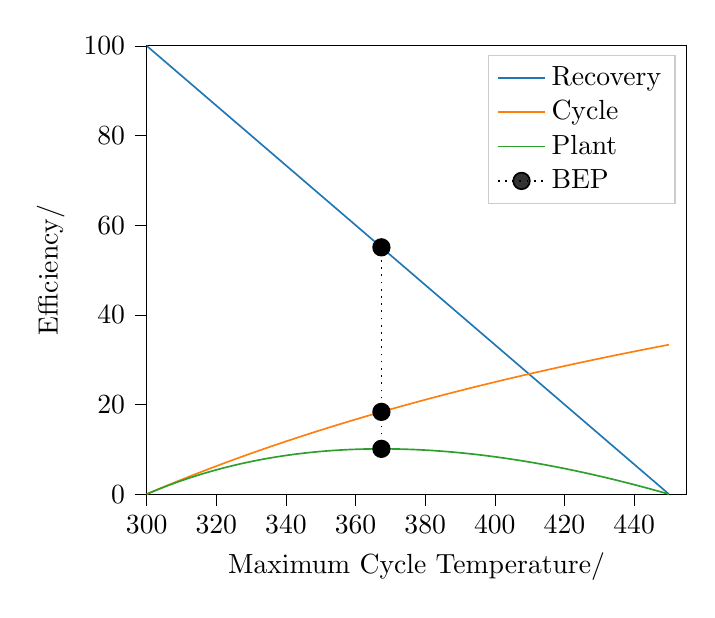
\begin{tikzpicture}

\definecolor{darkgray176}{RGB}{176,176,176}
\definecolor{darkorange25512714}{RGB}{255,127,14}
\definecolor{forestgreen4416044}{RGB}{44,160,44}
\definecolor{lightgray204}{RGB}{204,204,204}
\definecolor{steelblue31119180}{RGB}{31,119,180}

\begin{axis}[
legend cell align={left},
legend style={fill opacity=0.8, draw opacity=1, text opacity=1, draw=lightgray204},
tick align=outside,
tick pos=left,
x grid style={darkgray176},
xlabel={Maximum Cycle Temperature/\unit{\K}},
xmin=300, xmax=455,
xtick style={color=black},
y grid style={darkgray176},
ylabel={Efficiency/\unit{\percent}},
ymin=0, ymax=100,
ytick style={color=black}
]
\addplot [semithick, steelblue31119180]
table {%
300 100
303.061224489796 97.9591836734694
306.122448979592 95.9183673469388
309.183673469388 93.8775510204082
312.244897959184 91.8367346938776
315.30612244898 89.795918367347
318.367346938775 87.7551020408163
321.428571428571 85.7142857142857
324.489795918367 83.6734693877551
327.551020408163 81.6326530612245
330.612244897959 79.5918367346939
333.673469387755 77.5510204081633
336.734693877551 75.5102040816327
339.795918367347 73.469387755102
342.857142857143 71.4285714285714
345.918367346939 69.3877551020408
348.979591836735 67.3469387755102
352.040816326531 65.3061224489796
355.102040816327 63.265306122449
358.163265306122 61.2244897959184
361.224489795918 59.1836734693878
364.285714285714 57.1428571428572
367.34693877551 55.1020408163266
370.408163265306 53.0612244897959
373.469387755102 51.0204081632653
376.530612244898 48.9795918367347
379.591836734694 46.9387755102041
382.65306122449 44.8979591836735
385.714285714286 42.8571428571428
388.775510204082 40.8163265306123
391.836734693878 38.7755102040816
394.897959183673 36.734693877551
397.959183673469 34.6938775510204
401.020408163265 32.6530612244898
404.081632653061 30.6122448979592
407.142857142857 28.5714285714286
410.204081632653 26.5306122448979
413.265306122449 24.4897959183673
416.326530612245 22.4489795918367
419.387755102041 20.4081632653061
422.448979591837 18.3673469387755
425.510204081633 16.3265306122449
428.571428571429 14.2857142857143
431.632653061224 12.2448979591837
434.69387755102 10.2040816326531
437.755102040816 8.16326530612245
440.816326530612 6.12244897959185
443.877551020408 4.08163265306121
446.938775510204 2.0408163265306
450 0
};
\addlegendentry{Recovery}
\addplot [semithick, darkorange25512714]
table {%
300 0
303.061224489796 1.01010101010101
306.122448979592 1.99999999999999
309.183673469388 2.97029702970297
312.244897959184 3.92156862745098
315.30612244898 4.85436893203883
318.367346938775 5.76923076923076
321.428571428571 6.66666666666668
324.489795918367 7.54716981132075
327.551020408163 8.41121495327103
330.612244897959 9.25925925925926
333.673469387755 10.0917431192661
336.734693877551 10.9090909090909
339.795918367347 11.7117117117117
342.857142857143 12.5
345.918367346939 13.2743362831858
348.979591836735 14.0350877192982
352.040816326531 14.7826086956522
355.102040816327 15.5172413793103
358.163265306122 16.2393162393162
361.224489795918 16.9491525423729
364.285714285714 17.6470588235294
367.34693877551 18.3333333333333
370.408163265306 19.0082644628099
373.469387755102 19.672131147541
376.530612244898 20.3252032520325
379.591836734694 20.9677419354839
382.65306122449 21.6
385.714285714286 22.2222222222222
388.775510204082 22.8346456692913
391.836734693878 23.4375
394.897959183673 24.031007751938
397.959183673469 24.6153846153846
401.020408163265 25.1908396946565
404.081632653061 25.7575757575758
407.142857142857 26.3157894736842
410.204081632653 26.865671641791
413.265306122449 27.4074074074074
416.326530612245 27.9411764705882
419.387755102041 28.4671532846715
422.448979591837 28.9855072463768
425.510204081633 29.4964028776978
428.571428571429 30
431.632653061224 30.4964539007092
434.69387755102 30.9859154929577
437.755102040816 31.4685314685315
440.816326530612 31.9444444444444
443.877551020408 32.4137931034483
446.938775510204 32.8767123287671
450 33.3333333333333
};
\addlegendentry{Cycle}
\addplot [semithick, forestgreen4416044]
table {%
300 0
303.061224489796 0.989486703772414
306.122448979592 1.91836734693877
309.183673469388 2.78844210951708
312.244897959184 3.60144057623049
315.30612244898 4.35902516346344
318.367346938775 5.06279434850863
321.428571428571 5.71428571428572
324.489795918367 6.31497882171736
327.551020408163 6.86629792103758
330.612244897959 7.36961451247165
333.673469387755 7.82624976596143
336.734693877551 8.23747680890538
339.795918367347 8.60452289023718
342.857142857143 8.92857142857142
345.918367346939 9.21076395159835
348.979591836735 9.45220193340494
352.040816326531 9.65394853593611
355.102040816327 9.81703026038002
358.163265306122 9.94243851386709
361.224489795918 10.0311310965064
364.285714285714 10.0840336134454
367.34693877551 10.1020408163265
370.408163265306 10.0860178782257
373.469387755102 10.0368016058883
376.530612244898 9.95520159283226
379.591836734694 9.84200131665569
382.65306122449 9.69795918367347
385.714285714286 9.52380952380952
388.775510204082 9.32026353848626
391.836734693878 9.08801020408164
394.897959183673 8.82771713336497
397.959183673469 8.54003139717425
401.020408163265 8.22558030845926
404.081632653061 7.88497217068646
407.142857142857 7.51879699248121
410.204081632653 7.12762717027109
413.265306122449 6.71201814058957
416.326530612245 6.27250900360144
419.387755102041 5.80962311932072
422.448979591837 5.32386867790594
425.510204081633 4.81573924533842
428.571428571429 4.28571428571429
431.632653061224 3.73425966131134
434.69387755102 3.16182811152631
437.755102040816 2.56885971171686
440.816326530612 1.95578231292517
443.877551020408 1.32301196340605
446.938775510204 0.670953312831979
450 0
};
\addlegendentry{Plant}
\addplot [semithick, black, dotted, mark=*, mark size=3, mark options={solid}]
table {%
367.423461417477 10.1020514433644
367.423461417477 18.3503419072274
367.423461417477 55.0510257216822
};
\addlegendentry{BEP}
\end{axis}

\end{tikzpicture}

    %         \caption[The thermal recovery, cycle and plant efficiency for a Carnot cycle and a sensible heat dominated heat-source.]{The thermal recovery, cycle and plant efficiency as a function of the maximum cycle temperature for a Carnot cycle and a heat source characterised by a \(C_p\) of \qty{4}{\kilo\joule\per\kg\per\K} and a latent heat of \(x\Delta H_{fh}\) of \qty{0}{\kilo\joule\per\kg}}
    %         \label{fig:litrev_SaturatedSource_Carnot}
    %     \end{figure}

    %     Of course, Equation~\ref{eq:carnot_Topt} is only valid for cases where the resultant \(T_{cycle}^{max}\) is less than or equal to \(T_H\), this critical point (i.e. where \(T_{cycle}^{max}=T_H\)), is given by Equation~\ref{eq:carnot_crit_point}. 

    %     \begin{align}
    %        \frac{x\Delta H_{fg}}{C_p}_{crit} = T_H\left( \frac{T_H}{T_C} - 1 \right)\label{eq:carnot_crit_point}
    %     \end{align}


    %     \begin{figure}[H]
    %         \centering
    %         % This file was created with tikzplotlib v0.10.1.
\begin{tikzpicture}

\definecolor{crimson2143940}{RGB}{214,39,40}
\definecolor{darkgray176}{RGB}{176,176,176}
\definecolor{darkorange25512714}{RGB}{255,127,14}
\definecolor{forestgreen4416044}{RGB}{44,160,44}
\definecolor{lightgray204}{RGB}{204,204,204}
\definecolor{mediumpurple148103189}{RGB}{148,103,189}
\definecolor{steelblue31119180}{RGB}{31,119,180}

\begin{axis}[
legend cell align={left},
legend style={
  fill opacity=0.8,
  draw opacity=1,
  text opacity=1,
  at={(1.03,0.5)},
  anchor=west,
  draw=lightgray204
},
tick align=outside,
tick pos=left,
x grid style={darkgray176},
xlabel={Maximum Cycle Temperature/\unit{\K}},
xmin=300, xmax=455,
xtick style={color=black},
y grid style={darkgray176},
ylabel={Efficiency/\unit{\percent}},
ymin=0, ymax=40,
ytick style={color=black}
]
\addplot [semithick, steelblue31119180]
table {%
300 0
303.061224489796 0.989486703772414
306.122448979592 1.91836734693877
309.183673469388 2.78844210951708
312.244897959184 3.60144057623049
315.30612244898 4.35902516346344
318.367346938775 5.06279434850863
321.428571428571 5.71428571428572
324.489795918367 6.31497882171736
327.551020408163 6.86629792103758
330.612244897959 7.36961451247165
333.673469387755 7.82624976596143
336.734693877551 8.23747680890538
339.795918367347 8.60452289023718
342.857142857143 8.92857142857142
345.918367346939 9.21076395159835
348.979591836735 9.45220193340494
352.040816326531 9.65394853593611
355.102040816327 9.81703026038002
358.163265306122 9.94243851386709
361.224489795918 10.0311310965064
364.285714285714 10.0840336134454
367.34693877551 10.1020408163265
370.408163265306 10.0860178782257
373.469387755102 10.0368016058883
376.530612244898 9.95520159283226
379.591836734694 9.84200131665569
382.65306122449 9.69795918367347
385.714285714286 9.52380952380952
388.775510204082 9.32026353848626
391.836734693878 9.08801020408164
394.897959183673 8.82771713336497
397.959183673469 8.54003139717425
401.020408163265 8.22558030845926
404.081632653061 7.88497217068646
407.142857142857 7.51879699248121
410.204081632653 7.12762717027109
413.265306122449 6.71201814058957
416.326530612245 6.27250900360144
419.387755102041 5.80962311932072
422.448979591837 5.32386867790594
425.510204081633 4.81573924533842
428.571428571429 4.28571428571429
431.632653061224 3.73425966131134
434.69387755102 3.16182811152631
437.755102040816 2.56885971171686
440.816326530612 1.95578231292517
443.877551020408 1.32301196340605
446.938775510204 0.670953312831979
450 0
};
\addlegendentry{\(x\Delta H_{fg}=\)\qty{0}{\kilo\joule\per\kg}}
\addplot [semithick, darkorange25512714]
table {%
300 0
303.061224489796 0.998856843012683
306.122448979592 1.95547309833023
309.183673469388 2.8711034368743
312.244897959184 3.74695332678526
315.30612244898 4.5841814219068
318.367346938775 5.38390181247323
321.428571428571 6.14718614718616
324.489795918367 6.87506563517345
327.551020408163 7.56853293568915
330.612244897959 8.22854394282965
333.673469387755 8.85601947200899
336.734693877551 9.45184685444426
339.795918367347 10.0168814454529
342.857142857143 10.551948051948
345.918367346939 11.0578422841381
348.979591836735 11.5353318360837
352.040816326531 11.9851576994434
355.102040816327 12.4080353144393
358.163265306122 12.8046556617985
361.224489795918 13.175686299173
364.285714285714 13.5217723453018
367.34693877551 13.843537414966
370.408163265306 14.1415845075821
373.469387755102 14.416496852094
376.530612244898 14.6688387106506
379.591836734694 14.8991561433958
382.65306122449 15.1079777365492
385.714285714286 15.2958152958153
388.775510204082 15.463164507034
391.836734693878 15.6105055658627
394.897959183673 15.7383037781709
397.959183673469 15.8470101327244
401.020408163265 15.9370618476398
404.081632653061 16.0088828919998
407.142857142857 16.0628844839371
410.204081632653 16.0994655664165
413.265306122449 16.1190132618704
416.326530612245 16.1219033067773
419.387755102041 16.1085004672075
422.448979591837 16.0791589363018
425.510204081633 16.0342227145927
428.571428571429 15.974025974026
431.632653061224 15.8988934064922
434.69387755102 15.8091405576315
437.755102040816 15.7050741466326
440.816326530612 15.5869923727067
443.877551020408 15.4551852088798
446.938775510204 15.3099346837116
450 15.1515151515152
};
\addlegendentry{\(x\Delta H_{fg}=\)\qty{500}{\kilo\joule\per\kg}}
\addplot [semithick, forestgreen4416044]
table {%
300 0
303.061224489796 1.00237064522778
306.122448979592 1.96938775510203
309.183673469388 2.90210143463326
312.244897959184 3.80152060824329
315.30612244898 4.66861501882306
318.367346938775 5.50431711145996
321.428571428571 6.30952380952382
324.489795918367 7.08509819021948
327.551020408163 7.83187106618348
330.612244897959 8.55064247921391
333.673469387755 9.24218311177683
336.734693877551 9.90723562152134
339.795918367347 10.5465159036588
342.857142857143 11.1607142857143
345.918367346939 11.7504966588405
348.979591836735 12.3165055495883
352.040816326531 12.8593611357586
355.102040816327 13.3796622097115
358.163265306122 13.8779870922728
361.224489795918 14.3548945001729
364.285714285714 14.8109243697479
367.34693877551 15.2465986394558
370.408163265306 15.6624219935908
373.469387755102 16.0588825694212
376.530612244898 16.4364526298324
379.591836734694 16.7955892034233
382.65306122449 17.1367346938775
385.714285714286 17.4603174603175
388.775510204082 17.7667523702394
391.836734693878 18.0564413265306
394.897959183673 18.3297737699731
397.959183673469 18.5871271585557
401.020408163265 18.8288674248325
404.081632653061 19.0553494124923
407.142857142857 19.2669172932331
410.204081632653 19.4639049649711
413.265306122449 19.6466364323507
416.326530612245 19.8154261704682
419.387755102041 19.970579472665
422.448979591837 20.1123927832002
425.510204081633 20.2411540155631
428.571428571429 20.3571428571429
431.632653061224 20.460631060935
434.69387755102 20.551882724921
437.755102040816 20.631154559726
440.816326530612 20.6986961451247
443.877551020408 20.7547501759324
446.938775510204 20.7995526977914
450 20.8333333333333
};
\addlegendentry{\(x\Delta H_{fg}=\)\qty{1000}{\kilo\joule\per\kg}}
\addplot [semithick, crimson2143940]
table {%
300 0
303.061224489796 1.00534386248672
306.122448979592 1.9811616954474
309.183673469388 2.92833050966007
312.244897959184 3.84769292332317
315.30612244898 4.74005883159836
318.367346938775 5.60620697983335
321.428571428571 6.44688644688646
324.489795918367 7.2628180444892
327.551020408163 8.05469563814023
330.612244897959 8.82318739461596
333.673469387755 9.56893696081115
336.734693877551 10.2925645782789
339.795918367347 10.9946681375253
342.857142857143 11.6758241758242
345.918367346939 12.3365888220503
348.979591836735 12.9774986917844
352.040816326531 13.5990717357177
355.102040816327 14.2018080441726
358.163265306122 14.7861906103664
361.224489795918 15.3526860548652
364.285714285714 15.90174531351
367.34693877551 16.4338042909471
370.408163265306 16.949284481752
373.469387755102 17.4485935610057
376.530612244898 17.9321259460632
379.591836734694 18.4002633311389
382.65306122449 18.8533751962323
385.714285714286 19.2918192918193
388.775510204082 19.715942100644
391.836734693878 20.126079277865
394.897959183673 20.5225560707288
397.959183673469 20.9056877188745
401.020408163265 21.2757798363033
404.081632653061 21.6331287759859
407.142857142857 21.978021978022
410.204081632653 22.3107383022095
413.265306122449 22.6315483458341
416.326530612245 22.9407147474374
419.387755102041 23.2384924772829
422.448979591837 23.5251291151912
425.510204081633 23.8008651163841
428.571428571429 24.0659340659341
431.632653061224 24.3205629223866
434.69387755102 24.5649722510889
437.755102040816 24.7993764477281
440.816326530612 25.0239839525554
443.877551020408 25.2389974557462
446.938775510204 25.4446140943205
450 25.6410256410256
};
\addlegendentry{\(x\Delta H_{fg}=\)\qty{2000}{\kilo\joule\per\kg}}
\addplot [semithick, mediumpurple148103189]
table {%
300 0
303.061224489796 1.00741218753641
306.122448979592 1.98935226264418
309.183673469388 2.9465768227222
312.244897959184 3.87981279468309
315.30612244898 4.78975887526813
318.367346938775 5.677086888267
321.428571428571 6.5424430641822
324.489795918367 7.38644924745944
327.551020408163 8.20970403602319
330.612244897959 9.01278385750435
333.673469387755 9.79624398622633
336.734693877551 10.5606195047189
339.795918367347 11.3064262132585
342.857142857143 12.0341614906832
345.918367346939 12.7443051095005
348.979591836735 13.4373200080948
352.040816326531 14.1136530226457
355.102040816327 14.773735581189
358.163265306122 15.4179843620838
361.224489795918 16.046801918999
364.285714285714 16.660577274388
367.34693877551 17.259686483289
370.408163265306 17.8444931691685
373.469387755102 18.4153490334124
376.530612244898 18.9725943399629
379.591836734694 19.5165583765063
382.65306122449 20.0475598935226
385.714285714286 20.5659075224293
388.775510204082 21.0719001739689
391.836734693878 21.5658274179237
394.897959183673 22.0479698451676
397.959183673469 22.5185994130094
401.020408163265 22.9779797747177
404.081632653061 23.4263665940685
407.142857142857 23.8640078457012
410.204081632653 24.2911441020276
413.265306122449 24.7080088073877
416.326530612245 25.1148285401117
419.387755102041 25.511823263104
422.448979591837 25.8992065635328
425.510204081633 26.2771858821727
428.571428571429 26.6459627329192
431.632653061224 27.0057329129617
434.69387755102 27.3566867040754
437.755102040816 27.6990090654687
440.816326530612 28.0328798185941
443.877551020408 28.3584738243123
446.938775510204 28.6759611527756
450 28.9855072463768
};
\addlegendentry{\(x\Delta H_{fg}=\)\qty{4000}{\kilo\joule\per\kg}}
\addplot [semithick, black, dashed]
table {%
300 0
303.061224489796 1.01010101010101
306.122448979592 1.99999999999999
309.183673469388 2.97029702970297
312.244897959184 3.92156862745098
315.30612244898 4.85436893203883
318.367346938775 5.76923076923076
321.428571428571 6.66666666666668
324.489795918367 7.54716981132075
327.551020408163 8.41121495327103
330.612244897959 9.25925925925926
333.673469387755 10.0917431192661
336.734693877551 10.9090909090909
339.795918367347 11.7117117117117
342.857142857143 12.5
345.918367346939 13.2743362831858
348.979591836735 14.0350877192982
352.040816326531 14.7826086956522
355.102040816327 15.5172413793103
358.163265306122 16.2393162393162
361.224489795918 16.9491525423729
364.285714285714 17.6470588235294
367.34693877551 18.3333333333333
370.408163265306 19.0082644628099
373.469387755102 19.672131147541
376.530612244898 20.3252032520325
379.591836734694 20.9677419354839
382.65306122449 21.6
385.714285714286 22.2222222222222
388.775510204082 22.8346456692913
391.836734693878 23.4375
394.897959183673 24.031007751938
397.959183673469 24.6153846153846
401.020408163265 25.1908396946565
404.081632653061 25.7575757575758
407.142857142857 26.3157894736842
410.204081632653 26.865671641791
413.265306122449 27.4074074074074
416.326530612245 27.9411764705882
419.387755102041 28.4671532846715
422.448979591837 28.9855072463768
425.510204081633 29.4964028776978
428.571428571429 30
431.632653061224 30.4964539007092
434.69387755102 30.9859154929577
437.755102040816 31.4685314685315
440.816326530612 31.9444444444444
443.877551020408 32.4137931034483
446.938775510204 32.8767123287671
450 33.3333333333333
};
\addlegendentry{\(x\Delta H_{fg}=\infty\) \unit{\kilo\joule\per\kg}}
\addplot [semithick, black, dotted, mark=*, mark size=3, mark options={solid}]
table {%
367.423461417477 10.1020514433644
415.331193145904 16.1227686211609
450 20.8333333333333
450 25.6410256410256
450 28.9855072463768
450 33.3333333333333
};
\addlegendentry{BEP}
\end{axis}

\end{tikzpicture}

    %         \caption[The overall plant efficiency for different latent heats as a function of maximum cycle temperature.]{The overall plant efficiency as a function of the maximum cycle temperature for a Carnot cycle and a heat source characterised by a \(C_p\) of \qty{4}{\kilo\joule\per\kg\per\K} and different latent heats}
    %         \label{fig:litrev_GenericSource_Carnot}
    %     \end{figure}

    %     For the Triangular cycle, circumstances are somewhat different; due to the unique structure of the Triangular cycle, \(\eta_{recov}\) is equal to one for all maximum cycle temperatures. As such, the plant efficiency is equal to that of the triangular cycle, unaffected by latent heat of the heat source, and the optimum maximum cycle temperature is equal to the temperature of the heat source \(T_H\). 
        
    %     For this reason Triangular cycles are the ideal candidates for exploiting single phase or low latent heat heat sources. Comparing the overall plant efficiency of the Triangular and Carnot cycle plants for different amounts of latent heat, Triangular cycle can be seen to provide better overall plant efficiencies than the Carnot cycle plant for latent heats as high as \qty{900}{\kilo\joule\per\kg}. The critical ratio of latent heat to the specific heat capacity is given by Equation~\ref{eq:carnot_triangular_crit_point}. For combinations of latent heat and specific heat capacity in excess of this critical point, the Carnot cycle outperforms the Triangular cycle.

    %     \begin{align}
    %        \frac{x\Delta H_{fg}}{C_p}_{crit} = (T_H -T_C) * \frac{\eta_{cycle}^{triangular}}{\eta_{cycle}^{carnot}-\eta_{cycle}^{triangular}}\label{eq:carnot_triangular_crit_point}
    %     \end{align}

    %     \begin{figure}[H]
    %         \centering
    %         % This file was created with tikzplotlib v0.10.1.
\begin{tikzpicture}

\definecolor{crimson2143940}{RGB}{214,39,40}
\definecolor{darkgray176}{RGB}{176,176,176}
\definecolor{darkorange25512714}{RGB}{255,127,14}
\definecolor{forestgreen4416044}{RGB}{44,160,44}
\definecolor{lightgray204}{RGB}{204,204,204}
\definecolor{mediumpurple148103189}{RGB}{148,103,189}
\definecolor{sienna1408675}{RGB}{140,86,75}
\definecolor{steelblue31119180}{RGB}{31,119,180}

\begin{axis}[
legend cell align={left},
legend style={
  fill opacity=0.8,
  draw opacity=1,
  text opacity=1,
  at={(1.03,0.5)},
  anchor=west,
  draw=lightgray204
},
tick align=outside,
tick pos=left,
x grid style={darkgray176},
xlabel={Maximum Cycle Temperature/\unit{\K}},
xmin=300, xmax=455,
xtick style={color=black},
y grid style={darkgray176},
ylabel={Plant Efficiency/\unit{\percent}},
ymin=0, ymax=40,
ytick style={color=black}
]
\addplot [semithick, steelblue31119180]
table {%
300 0
303.061224489796 0.989486703772414
306.122448979592 1.91836734693877
309.183673469388 2.78844210951708
312.244897959184 3.60144057623049
315.30612244898 4.35902516346344
318.367346938775 5.06279434850863
321.428571428571 5.71428571428572
324.489795918367 6.31497882171736
327.551020408163 6.86629792103758
330.612244897959 7.36961451247165
333.673469387755 7.82624976596143
336.734693877551 8.23747680890538
339.795918367347 8.60452289023718
342.857142857143 8.92857142857142
345.918367346939 9.21076395159835
348.979591836735 9.45220193340494
352.040816326531 9.65394853593611
355.102040816327 9.81703026038002
358.163265306122 9.94243851386709
361.224489795918 10.0311310965064
364.285714285714 10.0840336134454
367.34693877551 10.1020408163265
370.408163265306 10.0860178782257
373.469387755102 10.0368016058883
376.530612244898 9.95520159283226
379.591836734694 9.84200131665569
382.65306122449 9.69795918367347
385.714285714286 9.52380952380952
388.775510204082 9.32026353848626
391.836734693878 9.08801020408164
394.897959183673 8.82771713336497
397.959183673469 8.54003139717425
401.020408163265 8.22558030845926
404.081632653061 7.88497217068646
407.142857142857 7.51879699248121
410.204081632653 7.12762717027109
413.265306122449 6.71201814058957
416.326530612245 6.27250900360144
419.387755102041 5.80962311932072
422.448979591837 5.32386867790594
425.510204081633 4.81573924533842
428.571428571429 4.28571428571429
431.632653061224 3.73425966131134
434.69387755102 3.16182811152631
437.755102040816 2.56885971171686
440.816326530612 1.95578231292517
443.877551020408 1.32301196340605
446.938775510204 0.670953312831979
450 0
};
\addlegendentry{\(x\Delta H_{fg}=\)\qty{0}{\kilo\joule\per\kg}}
\addplot [semithick, darkorange25512714]
table {%
300 0
303.061224489796 0.995549735045529
306.122448979592 1.9423769507803
309.183673469388 2.84192885074822
312.244897959184 3.69559588541299
315.30612244898 4.50471450716209
318.367346938775 5.27056976636808
321.428571428571 5.99439775910365
324.489795918367 6.6773879363066
327.551020408163 7.32068528345918
330.612244897959 7.92539237917389
333.673469387755 8.4925713404628
336.734693877551 9.02324566190113
339.795918367347 9.51840195537675
342.857142857143 9.97899159663865
345.918367346939 10.4059322844182
348.979591836735 10.8001095174912
352.040816326531 11.1623779946761
355.102040816327 11.4935629424183
358.163265306122 11.7944613742933
361.224489795918 12.0658432864671
364.285714285714 12.3084527928819
367.34693877551 12.5230092036815
370.408163265306 12.7102080501622
373.469387755102 12.8707220593155
376.530612244898 13.0052020808323
379.591836734694 13.1142779692522
382.65306122449 13.1985594237695
385.714285714286 13.2586367880486
388.775510204082 13.2950818122525
391.836734693878 13.3084483793517
394.897959183673 13.2992731976512
397.959183673469 13.2680764613538
401.020408163265 13.2153624808702
404.081632653061 13.1416202844774
407.142857142857 13.047324192835
410.204081632653 12.932934367777
413.265306122449 12.7988973367125
416.326530612245 12.6456464938917
419.387755102041 12.473602579718
422.448979591837 12.2831741392209
425.510204081633 12.0747579607383
428.571428571429 11.8487394957983
431.632653061224 11.6054932611342
434.69387755102 11.345383223712
437.755102040816 11.0687631696035
440.816326530612 10.7759770574897
443.877551020408 10.4673593575361
446.938775510204 10.1432353763423
450 9.80392156862745
};
\addlegendentry{\(x\Delta H_{fg}=\)\qty{250}{\kilo\joule\per\kg}}
\addplot [semithick, forestgreen4416044]
table {%
300 0
303.061224489796 0.998856843012683
306.122448979592 1.95547309833023
309.183673469388 2.8711034368743
312.244897959184 3.74695332678526
315.30612244898 4.5841814219068
318.367346938775 5.38390181247323
321.428571428571 6.14718614718616
324.489795918367 6.87506563517345
327.551020408163 7.56853293568915
330.612244897959 8.22854394282965
333.673469387755 8.85601947200899
336.734693877551 9.45184685444426
339.795918367347 10.0168814454529
342.857142857143 10.551948051948
345.918367346939 11.0578422841381
348.979591836735 11.5353318360837
352.040816326531 11.9851576994434
355.102040816327 12.4080353144393
358.163265306122 12.8046556617985
361.224489795918 13.175686299173
364.285714285714 13.5217723453018
367.34693877551 13.843537414966
370.408163265306 14.1415845075821
373.469387755102 14.416496852094
376.530612244898 14.6688387106506
379.591836734694 14.8991561433958
382.65306122449 15.1079777365492
385.714285714286 15.2958152958153
388.775510204082 15.463164507034
391.836734693878 15.6105055658627
394.897959183673 15.7383037781709
397.959183673469 15.8470101327244
401.020408163265 15.9370618476398
404.081632653061 16.0088828919998
407.142857142857 16.0628844839371
410.204081632653 16.0994655664165
413.265306122449 16.1190132618704
416.326530612245 16.1219033067773
419.387755102041 16.1085004672075
422.448979591837 16.0791589363018
425.510204081633 16.0342227145927
428.571428571429 15.974025974026
431.632653061224 15.8988934064922
434.69387755102 15.8091405576315
437.755102040816 15.7050741466326
440.816326530612 15.5869923727067
443.877551020408 15.4551852088798
446.938775510204 15.3099346837116
450 15.1515151515152
};
\addlegendentry{\(x\Delta H_{fg}=\)\qty{500}{\kilo\joule\per\kg}}
\addplot [semithick, crimson2143940]
table {%
300 0
303.061224489796 1.00237064522778
306.122448979592 1.96938775510203
309.183673469388 2.90210143463326
312.244897959184 3.80152060824329
315.30612244898 4.66861501882306
318.367346938775 5.50431711145996
321.428571428571 6.30952380952382
324.489795918367 7.08509819021948
327.551020408163 7.83187106618348
330.612244897959 8.55064247921391
333.673469387755 9.24218311177683
336.734693877551 9.90723562152134
339.795918367347 10.5465159036588
342.857142857143 11.1607142857143
345.918367346939 11.7504966588405
348.979591836735 12.3165055495883
352.040816326531 12.8593611357586
355.102040816327 13.3796622097115
358.163265306122 13.8779870922728
361.224489795918 14.3548945001729
364.285714285714 14.8109243697479
367.34693877551 15.2465986394558
370.408163265306 15.6624219935908
373.469387755102 16.0588825694212
376.530612244898 16.4364526298324
379.591836734694 16.7955892034233
382.65306122449 17.1367346938775
385.714285714286 17.4603174603175
388.775510204082 17.7667523702394
391.836734693878 18.0564413265306
394.897959183673 18.3297737699731
397.959183673469 18.5871271585557
401.020408163265 18.8288674248325
404.081632653061 19.0553494124923
407.142857142857 19.2669172932331
410.204081632653 19.4639049649711
413.265306122449 19.6466364323507
416.326530612245 19.8154261704682
419.387755102041 19.970579472665
422.448979591837 20.1123927832002
425.510204081633 20.2411540155631
428.571428571429 20.3571428571429
431.632653061224 20.460631060935
434.69387755102 20.551882724921
437.755102040816 20.631154559726
440.816326530612 20.6986961451247
443.877551020408 20.7547501759324
446.938775510204 20.7995526977914
450 20.8333333333333
};
\addlegendentry{\(x\Delta H_{fg}=\)\qty{1000}{\kilo\joule\per\kg}}
\addplot [semithick, mediumpurple148103189]
table {%
300 0
303.061224489796 1.00534386248672
306.122448979592 1.9811616954474
309.183673469388 2.92833050966007
312.244897959184 3.84769292332317
315.30612244898 4.74005883159836
318.367346938775 5.60620697983335
321.428571428571 6.44688644688646
324.489795918367 7.2628180444892
327.551020408163 8.05469563814023
330.612244897959 8.82318739461596
333.673469387755 9.56893696081115
336.734693877551 10.2925645782789
339.795918367347 10.9946681375253
342.857142857143 11.6758241758242
345.918367346939 12.3365888220503
348.979591836735 12.9774986917844
352.040816326531 13.5990717357177
355.102040816327 14.2018080441726
358.163265306122 14.7861906103664
361.224489795918 15.3526860548652
364.285714285714 15.90174531351
367.34693877551 16.4338042909471
370.408163265306 16.949284481752
373.469387755102 17.4485935610057
376.530612244898 17.9321259460632
379.591836734694 18.4002633311389
382.65306122449 18.8533751962323
385.714285714286 19.2918192918193
388.775510204082 19.715942100644
391.836734693878 20.126079277865
394.897959183673 20.5225560707288
397.959183673469 20.9056877188745
401.020408163265 21.2757798363033
404.081632653061 21.6331287759859
407.142857142857 21.978021978022
410.204081632653 22.3107383022095
413.265306122449 22.6315483458341
416.326530612245 22.9407147474374
419.387755102041 23.2384924772829
422.448979591837 23.5251291151912
425.510204081633 23.8008651163841
428.571428571429 24.0659340659341
431.632653061224 24.3205629223866
434.69387755102 24.5649722510889
437.755102040816 24.7993764477281
440.816326530612 25.0239839525554
443.877551020408 25.2389974557462
446.938775510204 25.4446140943205
450 25.6410256410256
};
\addlegendentry{\(x\Delta H_{fg}=\)\qty{2000}{\kilo\joule\per\kg}}
\addplot [semithick, sienna1408675]
table {%
300 0
303.061224489796 1.00741218753641
306.122448979592 1.98935226264418
309.183673469388 2.9465768227222
312.244897959184 3.87981279468309
315.30612244898 4.78975887526813
318.367346938775 5.677086888267
321.428571428571 6.5424430641822
324.489795918367 7.38644924745944
327.551020408163 8.20970403602319
330.612244897959 9.01278385750435
333.673469387755 9.79624398622633
336.734693877551 10.5606195047189
339.795918367347 11.3064262132585
342.857142857143 12.0341614906832
345.918367346939 12.7443051095005
348.979591836735 13.4373200080948
352.040816326531 14.1136530226457
355.102040816327 14.773735581189
358.163265306122 15.4179843620838
361.224489795918 16.046801918999
364.285714285714 16.660577274388
367.34693877551 17.259686483289
370.408163265306 17.8444931691685
373.469387755102 18.4153490334124
376.530612244898 18.9725943399629
379.591836734694 19.5165583765063
382.65306122449 20.0475598935226
385.714285714286 20.5659075224293
388.775510204082 21.0719001739689
391.836734693878 21.5658274179237
394.897959183673 22.0479698451676
397.959183673469 22.5185994130094
401.020408163265 22.9779797747177
404.081632653061 23.4263665940685
407.142857142857 23.8640078457012
410.204081632653 24.2911441020276
413.265306122449 24.7080088073877
416.326530612245 25.1148285401117
419.387755102041 25.511823263104
422.448979591837 25.8992065635328
425.510204081633 26.2771858821727
428.571428571429 26.6459627329192
431.632653061224 27.0057329129617
434.69387755102 27.3566867040754
437.755102040816 27.6990090654687
440.816326530612 28.0328798185941
443.877551020408 28.3584738243123
446.938775510204 28.6759611527756
450 28.9855072463768
};
\addlegendentry{\(x\Delta H_{fg}=\)\qty{4000}{\kilo\joule\per\kg}}
\addplot [semithick, black, dashed]
table {%
300 0
303.061224489796 1.01010101010101
306.122448979592 1.99999999999999
309.183673469388 2.97029702970297
312.244897959184 3.92156862745098
315.30612244898 4.85436893203883
318.367346938775 5.76923076923076
321.428571428571 6.66666666666668
324.489795918367 7.54716981132075
327.551020408163 8.41121495327103
330.612244897959 9.25925925925926
333.673469387755 10.0917431192661
336.734693877551 10.9090909090909
339.795918367347 11.7117117117117
342.857142857143 12.5
345.918367346939 13.2743362831858
348.979591836735 14.0350877192982
352.040816326531 14.7826086956522
355.102040816327 15.5172413793103
358.163265306122 16.2393162393162
361.224489795918 16.9491525423729
364.285714285714 17.6470588235294
367.34693877551 18.3333333333333
370.408163265306 19.0082644628099
373.469387755102 19.672131147541
376.530612244898 20.3252032520325
379.591836734694 20.9677419354839
382.65306122449 21.6
385.714285714286 22.2222222222222
388.775510204082 22.8346456692913
391.836734693878 23.4375
394.897959183673 24.031007751938
397.959183673469 24.6153846153846
401.020408163265 25.1908396946565
404.081632653061 25.7575757575758
407.142857142857 26.3157894736842
410.204081632653 26.865671641791
413.265306122449 27.4074074074074
416.326530612245 27.9411764705882
419.387755102041 28.4671532846715
422.448979591837 28.9855072463768
425.510204081633 29.4964028776978
428.571428571429 30
431.632653061224 30.4964539007092
434.69387755102 30.9859154929577
437.755102040816 31.4685314685315
440.816326530612 31.9444444444444
443.877551020408 32.4137931034483
446.938775510204 32.8767123287671
450 33.3333333333333
};
\addlegendentry{\(x\Delta H_{fg}=\infty\)\unit{\kilo\joule\per\kg}}
\addplot [semithick, red]
table {%
300 0
303.061224489796 0.507614213197967
306.122448979592 1.01010101010101
309.183673469388 1.50753768844221
312.244897959184 2
315.30612244898 2.48756218905472
318.367346938775 2.97029702970297
321.428571428571 3.44827586206897
324.489795918367 3.92156862745098
327.551020408163 4.39024390243902
330.612244897959 4.85436893203883
333.673469387755 5.31400966183575
336.734693877551 5.76923076923077
339.795918367347 6.2200956937799
342.857142857143 6.66666666666666
345.918367346939 7.1090047393365
348.979591836735 7.54716981132076
352.040816326531 7.98122065727699
355.102040816327 8.41121495327102
358.163265306122 8.83720930232558
361.224489795918 9.25925925925926
364.285714285714 9.67741935483871
367.34693877551 10.0917431192661
370.408163265306 10.5022831050228
373.469387755102 10.9090909090909
376.530612244898 11.3122171945701
379.591836734694 11.7117117117117
382.65306122449 12.1076233183856
385.714285714286 12.5
388.775510204082 12.8888888888889
391.836734693878 13.2743362831858
394.897959183673 13.6563876651982
397.959183673469 14.0350877192982
401.020408163265 14.410480349345
404.081632653061 14.7826086956522
407.142857142857 15.1515151515151
410.204081632653 15.5172413793103
413.265306122449 15.8798283261803
416.326530612245 16.2393162393162
419.387755102041 16.5957446808511
422.448979591837 16.9491525423729
425.510204081633 17.2995780590717
428.571428571429 17.6470588235294
431.632653061224 17.9916317991632
434.69387755102 18.3333333333333
437.755102040816 18.6721991701245
440.816326530612 19.0082644628099
443.877551020408 19.3415637860082
446.938775510204 19.672131147541
450 20
};
\addlegendentry{Triangular Cycle}
\addplot [semithick, black, dotted]
table {%
367.423461417477 10.1020514433644
392.109678533953 13.3085378503971
415.331193145904 16.1227686211609
450 20.8333333333333
450 25.6410256410256
450 28.9855072463768
450 33.3333333333333
};
\addlegendentry{BEP}
\end{axis}

\end{tikzpicture}

    %         \caption[The overall plant efficiency for different latent heats as a function of maximum cycle temperature for a Carnot and Triangular cycle.]{The overall plant efficiency as a function of the maximum cycle temperature for a Carnot cycle and a Triangular cycle for heat sources of different latent heat and a constant specific heat capacity \(C_p\) of \qty{4}{\kilo\joule\per\kg\per\K}.}
    %         \label{fig:litrev_GenericSource_Carnot_vs_Triangular}
    %     \end{figure}

    %     In summary, the overall plant efficiency of a binary plant depends not only on the efficiency of the thermodynamic cycle but also on the efficiency of thermal recovery from the heat source. Even though triangular cycle, has a low cycle efficiency, it is best suited for single phase source or two-phase sources with low amounts of latent heat, because of its high, and constant thermal recovery efficiency. The Carnot cycle achieves higher cycle efficiencies, however, generally operates at lower thermal recovery efficiencies, which reduce the overall plant efficiency. In this respect, the Carnot cycle is better suited for two-phase sources with large latent heat, due to the increased thermal recovery efficiency. The cut-off between the two is given by Equation~\ref{eq:carnot_triangular_crit_point}.


\section{NCG Handling}
    \label{sec:litrev_NCG_handling}

    The presence of \ac{NCG} in geofluids can pose a number of issues for the operation of geothermal power plants. For instance, expelling the \ac{NCG} liberated and expanded as part of \ac{DSC} geothermal power plants can be energy intensive and technically challenging. As most geothermal \ac{DSC} power plants expand the geofluid to sub-atmospheric conditions, at a minimum the \ac{NCG} must be re-pressurised to atmospheric conditions to allow the \ac{NCG} to be vented to atmosphere.

    Where the \ac{NCG} contains harmful constituents such as mercury or hydrogen sulfide, further treatment of the \ac{NCG} maybe required before it can be safely released into the environment. An example of this is the AMIS process designed by \emph{ENEL} to remove mercury and hydrogen sulfide from the \ac{NCG} effluent streams. During the AMIS process, mercury is removed using selenium or activated carbon adsorbents, and hydrogen sulfide is first catalytically oxidised to sulfur dioxide and then stripped using an alkaline solution (e.g. dilute ammonia or sodium hydroxide solution) \cite{Baldacci2005, Manzella2018}.

    With regards to \ac{NCG} with significant \ac{GWP}, there are two schools of thought on whether venting to atmosphere is an option. On the one hand, venting \ac{NCG} to atmosphere represents an obvious source of greenhouse gas emissions that should be prevented. In fact some geothermal power plants in Türkiye have carbon footprints as \qty{900}{\kg\per\mega\watt} to \qty{1400}{\kg\per\mega\watt}, which is comparable to coal-fired power stations.
    
    On other hand, such emissions do also occur naturally in the absence of geothermal power plants, for example from surface features like fumaroles. In this respect, if the emissions of a geothermal power or heat plant reduce the natural emissions by the same amount, the overall emissions from the geothermal site are unchanged. That being said, tracking and quantifying emissions across a wide area is no trivial task, as illustrated from attempts tracking methane leakage from active as well as abandoned oil and gas wells \cite{Collins2022}. While some countries, like Italy \cite{Armannsson2003} and Türkiye \cite{Baba2022}, have taken the stance that geothermal power plants do not increase the overall emissions, this view is not shared universally and in, for instance, Iceland efforts are taken to actively reduce \ac{NCG} emissions to reduce the carbon foot print \cite{Sigfusson2018}.
    
    At the Hellisheiði geothermal power plant in Iceland, \emph{CarbFix} have trialled the dissolution, re-injection and sequestration of \ac{NCG} using their \emph{Carbfix} process\cite{CarbFix2024}. At Hellisheiði, geothermal power is generated by means of a dual flash \ac{DSC} from a geofluid with carbon dioxide and hydrogen sulfide impurities (the \ac{NCG} comprises about \qty{5}{\percent} of the steam mass flow rate \cite{Sigfusson2018}). Following the expansion and cooling the \ac{NCG} is extracted using vacuum pumps. The \ac{NCG} stream is then pressurised and fed to an absorption column (at a temperature of \qty{293}{\K} or \qty{20}{\degreeCelsius}, and a pressure of \qty{6}{\bar}) \cite{Gunnarsson2018} to dissolve in geofluid condensate. The left over \ac{NCG} is vented the the atmosphere. The saturated gas-charged condensate is then injected at depth into the brine injection wellbore. 

    The basalt formations of the Hellisheiði field provide a natural mechanism for the long-term sequestration of carbon dioxide within the reservoir \cite{CarbFix2024, Gunnarsson2018}. That being said, it is important to ensure that mineralisation does not occur in close vicinity of the injections wells as this could result in clogging and reduce the injectivity in the long-term. Nevertheless, since 2014 the \emph{CarbFix} project at Hellisheiði have injected over \qty{100,000}{\tonne} of carbon dioxide \cite{CarbFix2024}.

    The main drawback from this approach is that the solubility of carbon dioxide in water at surface temperatures and pressures is low (at \emph{CarbFix} the maximum mole fraction of carbon dioxide in the re-injected water phase is just \qty{0.38}{\percent}). As the solubility of carbon dioxide increases with temperature and pressure, it is consequently not possible to dissolve and re-inject all of the produced carbon dioxide. In fact, this is already seen at \emph{CarbFix}, where only around \qty{35}{\percent} of the produced carbon dioxide is re-injected \cite{Sigfusson2018}.

    The main challenge to direct-injection of excess \ac{NCG} is its low density compared to brines, which leads to extremely high \ac{WHP}s being required to inject the \ac{NCG} into the reservoir formation. For example, as a rough approximation, neglecting frictional losses and temperature changes, injecting \qty{493}{\K} (\qty{20}{\degreeCelsius}) into a static water column at a depth of just \qty{500}{m} requires \ac{WHP} in excess off \qty{45}{\bar} (assuming ideal gas behaviour of the carbon dioxide phase). This is investigated in further detail in Section~\ref{sec:prosim_NCGhandling_Pinj}.

    \begin{align}
        P_{brine} = P_{wh,\;brine} + \rho_{brine}*g*h
    \end{align}
    \begin{align}
        P_{ncg} = P_{wh,\;ncg} * \exp{\frac{M_r*g*h}{RT}}
    \end{align}
    \begin{align}
        P_{wh,\;ncg} = (P_{wh,\;brine} + \rho_{brine}*g*h) * \exp{-\frac{M_r*g*h}{RT}}
    \end{align}
    \begin{align}
        P_{wh,\;ncg} = (1*10^5 + 1000*9.81*500) * \exp{\left(-\frac{0.044*9.81*500}{8.314 * 293}\right)} = 4.58*10^6 Pa
    \end{align}

    For reference, at these conditions the solubility has increased to \qty{2.37}{\percent} on a mole fraction basis. In principle, this could be used to dissolve the remaining carbon dioxide at Hellisheiði. In fact \citeauthor{Leontidis2023} \cite{Leontidis2023} conducted steady-state and transient simulations on the re-injection of \ac{NCG} into the reservoir considering various injection strategies, such as mixing of the \ac{NCG} and brine at the surface (i.e. two-phase injection), co-axial injection through a central pipe and surrounding annular space, as well as co-axial injection with mixing at depth. While their results suggest that mixing at depth may be possible and an attractive strategy for reducing surface compression power, particularly for low \ac{NCG} content, the authors highlight the importance of the underlying thermophysical property models. However, given that the simulation tools used in this study (i.e. \emph{PipeSim}, \emph{OLGA}, etc.) were originally developed for the oil and gas industry and are therefore used out of context, further investigations into the role of the following items are required:

    \begin{description}
        \item[Flow Correlations] The flow correlations used to determine the liquid-hold (e.g. Hagedorn \& Brown \cite{Hagedorn1965}) have generally been developed for upward vertical flow. However, in this case the flow is vertically downwards, and as such the buoyancy forces are now opposed to the direction of motion, which could affect the phase distribution and thus the liquid hold-up. This is particularly important because of the tendency of gas bubbles tend to coalesce into large bubbles, reducing surface tension and increasing buoyancy effects.  
        \item[Equilibration] When mixing \ac{NCG} and brine at depth, there may be significant barriers to mass transfer (e.g. due to limited interfacial area). As such, the common assumption of instantaneous equilibration (and hence dissolution of \ac{NCG}) may no longer be valid, leading to an overestimation of the liquid hold-up within the wellbore. Further simulations assuming no dissolution of \ac{NCG} in the brine even when in thermodynamic non-equilibrium could help assess the importance of these mass transfer effects.
    \end{description}
    
    Alternatively, owing to the low critical temperature, where the required wellhead pressure exceeds about \qty{60}{\bar} carbon dioxide could be liquefied at ambient temperatures. This has two advantages: 1) further compression requires significantly less power because liquid carbon dioxide is less compressible, 2) the higher density of liquid carbon dioxide adds significant static pressure in the wellbore, and 3) as the temperature and pressure increase, the liquid transitions to the supercritical state.
        
    As an alternative to re-injecting the \ac{NCG} into the reservoir, depending on the composition, it may be possible to upgrade the \ac{NCG} to commercial products. For example, where carbon dioxide is the main constituent, \ac{NCG} could be purified and converted to dry ice or used in beverages \cite{Baba2022}, provided there is a market and the capital investment is not prohibitive. There may also be niche applications, such as reusing carbon dioxide locally as an inhibitor to acidify the returns brine to prevent scale formation, as reported by \citeauthor{Topcu2019} \cite{Topcu2019}.

\section{Scale Handling}
    \label{sec:litrev_scale_handling}

        The geofluids are created over geological timescales, during which surface water resides in the geothermal reservoir and chemically equilibrates with the surrounding formation, causing minerals to leach from the formation \cite{DiPippo2016}. However, once the geofluid is produced from the reservoir and its temperature, pressure and composition are changed, this may cause the equilibrium to shift, causing minerals to precipitate. These mineral precipitates, commonly referred to as scales, can then deposit in the production system (i.e. wellbores, separators, heat exchange equipment) and impede the performance of the geothermal power plants. Calcite, Silica and sulphate scales are commonly encountered across the geothermal industry \cite{LuoKottsova2023}.

    \subsection{Calcite Scale}
        Calcite \ce{CaCO3} is a common mineral in geofluids from carbonate reservoirs. Due to its negatively sloped solubility curve (with respect to temperature), temperature reduction induced scaling is not typically an issue in a geothermal setting, as the solubility increases as the temperature is reduced.
    
        However, the solubility of calcite is also strongly dependent on the amount of carbon dioxide dissolved in the geofluid and the pH of the aqueous phase. Once the geofluid reaches its boiling point, or is flashed in the power plant, the resulting gas phase is enriched in carbon dioxide, which raises the pH and almost instantaneously causes calcite to precipitate. Such scaling is common carbonate fields, where the geofluids boils within the well-bores or surface, resulting in the thick calcite deposits that can incur significant pressure losses or even cause blockages\cite{DiPippo2016}. Acidisation or mechanical cleaning maybe used to manage calcite scaling once deposits become significant.

    \subsection{Silica Scale}
        Silica \ce{SiO2} is a common mineral found in geofluids, and exists in different crystalline structures, such as an amorphous state or as quartz in a highly crystalline state. While all forms of silica have a positively sloped solubility curve (with respect to temperature), the absolute solubility varies between the different forms, for example amorphous silica has a higher solubility in water than quartz\cite{DiPippo2016}. This puts both binary \ac{ORC} and \ac{DSC} with flash geothermal power plants at risk from silica scaling. Reductions in temperature (e.g. in the \ac{PHE}) or concentration of geofluid (e.g. steam removed by flashing) can result in the geofluid becoming supersaturated in silica. Silica scaling prevention is simpler in binary plants, as the geofluid is not concentrated by flashing stages, meaning that by simply managing the re-injection temperature supersaturated conditions can be prevented.   
    
        In terms of mitigation, strategies are to either prevent supersaturation by raising the pH to above \num{7}, or manage the kinetics of silica precipitation. For instance, reducing the speed of precipitation, may allow sufficient time for the geofluid to be re-injected into the reservoir, where any precipitate will eventually be dissolved. Kinetic inhibition could be achieved by pH control, by maintaining either low pH (<5.5) or high pH (>9.0) \cite{DiPippo2016}. An alternative approach is to achieve a controlled precipitation by increasing the rate of precipitation, and to remove the excess silica, re-injecting under-saturated geofluid into the reservoir \cite{DiPippo2016}.
        
\section{Turbines}
\label{sec:prosim_litrev_turbine}
    Turbines are used to convert the thermal energy contained within the working fluid into mechanical energy. The following subsections aim to provide background on the working principle, internal configuration, and types of turbines. 

    \subsection{Working Principle}
        Within the turbine, nozzles direct high velocity streams onto a solid element, called a blade, which deflects the fluid, Figure~\ref{fig:prosim_litrev_blade_velocity}. The change in momentum (i.e. \(v_{in}\) to \(v_{out}\)) imparts a resultant force on the blade opposite in the direction of the change in momentum. The blades are attached to a central shaft, such that resultant force manifests as a torque, causing the shaft to rotate. This rotation can then be used to drive a generator \cite{Dick2015, Smith2005}.
    
        \begin{figure}[H]
            \centering
            % \includesvg[width=0.45\columnwidth]{Content/PowGen/Figures/Turbine/VelocityTrianglesSchematic.svg}
            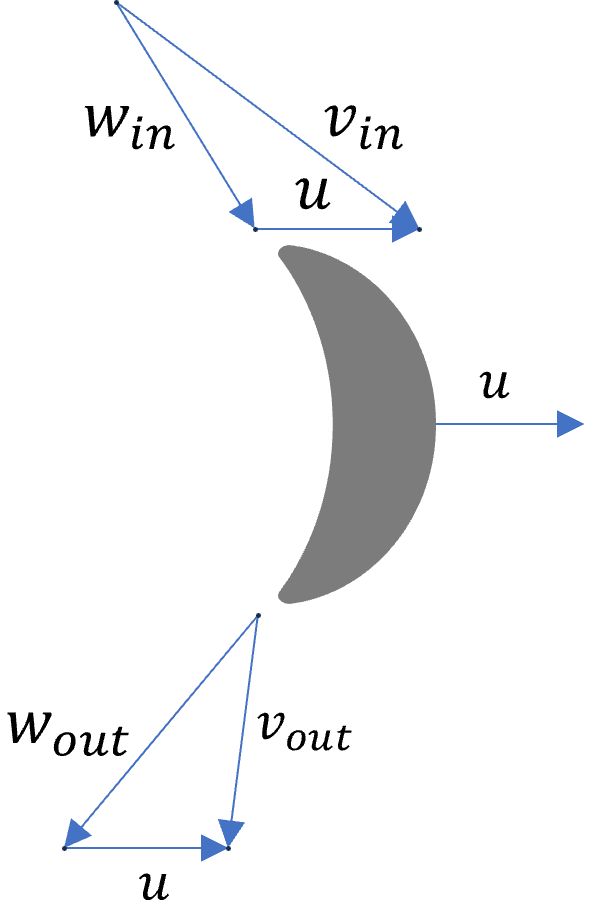
\includegraphics{Content/PowGen/Figures/Turbine/VelocityTrianglesSchematic.png}
            \caption{Fluid, blade and relative velocity vectors at the inlet and outlet of the blade.}
            \label{fig:prosim_litrev_blade_velocity}
        \end{figure}
    
        The maximum work, \(\Dot{w}\) generated by a turbine can be obtained from the Euler equation, Equation~\ref{eq:EulerEq}, or its alternate form, Equation~\ref{eq:AlternateEulerEq}, where \(v\) is the absolute fluid velocity, \(u\) is the tangential velocity of the blade, and \(w\) is the relative velocity from the perspective of the blade.
        
        \begin{align}
            \Dot{w} = \vec{u}_{in} \cdot \vec{c}_{in} - \vec{u}_{in}\cdot \vec{c}_{in} \label{eq:EulerEq}
        \end{align}
        \begin{align}
            \Dot{w} = \frac{v_{in}^2 - v_{out}^2}{2} + \frac{u_{in}^2-u_{out}^2}{2} - \frac{w_{in}^2-w_{out}^2}{2} \label{eq:AlternateEulerEq}
        \end{align}
    
        Velocity triangles, Figure~\ref{fig:prosim_litrev_velocity_triangles}, summarise the inlet and outlet velocity vectors and are an important tool for and optimising the  energy conversion.  
    
        \begin{figure}[H]
            \centering
            % \includesvg[width=0.45\columnwidth]{Content/PowGen/Figures/Turbine/VelocityTriangles.svg}
            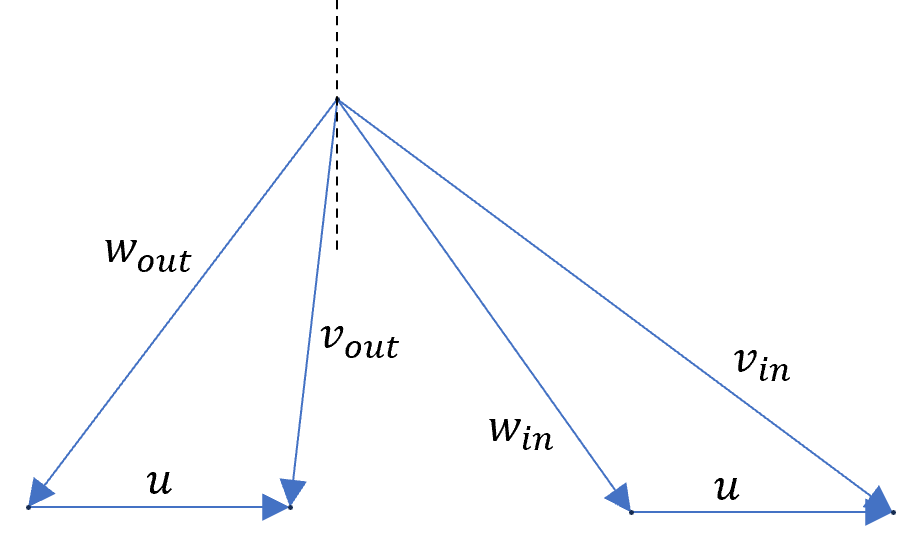
\includegraphics{Content/PowGen/Figures/Turbine/VelocityTriangles.png}
            \caption{Velocity Triangles.}
            \label{fig:prosim_litrev_velocity_triangles}
        \end{figure}
    
    \subsection{Impulse vs. Reaction Stages}
        To maximise the efficiency, the expansion is broken down into a number of stages, allowing the nozzles and blades to be specifically designed for the fluid and velocities at various stages of expansion. Each stage is comprised of a static stator, containing the nozzles, and the rotating rotor, containing the blades. There are two different types of turbine stages, impulse and reaction stages, the main difference being the mechanisms by which the fluid imparts the resultant force on the blades.
        
        In an impulse stage, Figure~\ref{fig:prosim_litrev_impulse}, the fluid is expanded in the stator nozzles, reducing the fluid pressure but increasing the volumetric flow rate and in turn the velocity of the fluid, Figure~\ref{fig:prosim_litrev_impulse_profile}. The fluid is then directed onto the blades, which deflect the fluid, and the change in momentum imparts the resultant force on the blade. In an ideal impulse stage, the fluid pressure in rotor section remains constant, such that only the kinetic energy is transferred to the blade/central shaft. 
        
        \begin{figure}[H]
            \centering
            \subfloat[Impulse stage.\label{fig:prosim_litrev_impulse}]{
                \includesvg[width=0.45\columnwidth]{Content/PowGen/Figures/Turbine/ImpulseStage.svg}
            }
            \quad
            \subfloat[Fluid pressure and velocity profile.\label{fig:prosim_litrev_impulse_profile}]{
                \includesvg[width=0.35\columnwidth]{Content/PowGen/Figures/Turbine/ImpulseStageProfiles.svg}
            }
            \caption[Configuration of an impulse turbine stage and the corresponding fluid pressure and velocity profiles.]{Configuration of an impulse turbine stage and the corresponding fluid pressure and velocity profiles. Adapted from \cite{Dick2015, Smith2005}}
            \label{fig:prosim_litrev_impulse_turbine_stage}
        \end{figure}
        
        In a reaction stage, Figure~\ref{fig:prosim_litrev_impulse}, the fluid is partially expanded in the stator nozzles and then directed onto the blades. Similarly to the impulse stage the fluid imparts some momentum on the blades, but is also expanded further, increasing its velocity, thus creating an area of low pressure on the back of the blades. This configuration allows both kinetic and pressure energy to be transferred to the shaft.
        
        \begin{figure}[H]
            \centering
            \subfloat[Reaction stage.\label{fig:prosim_litrev_reaction}]{
                \includesvg[width=0.45\columnwidth]{Content/PowGen/Figures/Turbine/ReactionStage.svg}
            }
            \quad
            \subfloat[Fluid pressure and velocity profile.\label{fig:prosim_litrev_reaction_profile}]{
                \includesvg[width=0.35\columnwidth]{Content/PowGen/Figures/Turbine/ReactionStageProfiles.svg}
            }
            \caption[Configuration of a reaction turbine stage and the corresponding fluid pressure and velocity profiles.]{Configuration of a reaction turbine stage and the corresponding fluid pressure and velocity profiles. Adapted from \cite{Dick2015, Smith2005}}
            \label{fig:prosim_litrev_reaction_turbine_stage}
        \end{figure}

        Impulse stages are typically used for small turbines or the high pressure stages of larger turbines. Reaction stages are used for low pressure and high through-put applications \cite{Smith2005}.    

    \subsection{Types of Turbines}

         \subsubsection{Axial Inflow, Axial Outflow}
            In axial turbines the fluid enters and exits the turbine parallel to the central axis, Figute~\ref{fig:prosim_litrev_axial_turbine}. Many commercial steam turbines utilise this design, as it can be readily extended to accommodate a large number of stages. The lessons from many decades of steam turbine operation can also be translated to the significantly smaller \ac{ORC} turbines, with this configuration being used extensively by \ac{ORC} system manufactures like Turboden \cite{Turboden2024} and Ormat \cite{Ormat2024, Buchanan2010}.

            \begin{figure}[H]
                \centering
                \includesvg[width=0.45\columnwidth]{Content/PowGen/Figures/Turbine/AxialTurbine.svg}
                \caption{Inlet and outlet streams of an axial turbine.}
                \label{fig:prosim_litrev_axial_turbine}
            \end{figure}
    
        \subsubsection{Radial Inflow}
            In a radial inflow, the fluid enters the turbine perpendicular to the central shaft along the outer perimeter, similar to a centrifugal compressor in reverse flow \cite{Boyce2012}. Unlike axial turbines, where the tangential velocity of the blades is constant (i.e. \(u_{in}=u_{out}\)), in this configuration due to the decreasing radius the tangential blade velocity at the outlet is lower than at the inlet (i.e. \(u_{in}>u_{out}\)), allowing the second term of Equation~\ref{eq:AlternateEulerEq} to be larger, leading to higher turbine efficiencies.

            % This configuration is similar to gas compressors, which are fed axially and discharge radially, albeit in reverse, 

            % \begin{itemize}
            %     \item (see Walraven for citation)
            %         used by Atlas Copco and Triogen 
            %         "centripetal turbine" - often a reverse action centrifugal compressor
            %         favourable velocity triangles, can yield high efficiencies (82 to 90\%) 
            % \end{itemize}

            \begin{figure}[H]
                \centering
                \includesvg[width=0.45\columnwidth]{Content/PowGen/Figures/Turbine/RadialInflowAxialOutflow.svg}
                \caption{Inlet and outlet streams of a radial inflow turbine.}
                \label{fig:prosim_litrev_RadialAxial_turbine}
            \end{figure}

        \subsubsection{Radial Outflow}
            The Ljungström brothers \cite{Dick2015} first proposed an axial inflow-radial outflow configuration, with the working fluid entering parallel to the central shaft, expanding radially through the turbine and then exiting perpendicular to the central shaft along the perimeter.

            \begin{figure}[H]
                \centering
                \includesvg[width=0.45\columnwidth]{Content/PowGen/Figures/Turbine/AxialInflowRadialOutflow.svg}
                \caption{Inlet and outlet streams of a radial-outflow turbine.}
                \label{fig:prosim_litrev_AxialRadial_turbine}
            \end{figure}

            An advantage of this design is that the flow area naturally increases as the fluid progresses radially through the turbine, thus, in principle allowing the turbine to be more compact. In axial turbines on the hand, the diameter must be increased along the length of the turbine to accommodate the increasing volume rate and prevent supersonic velocities. However, the increasing flowing radius also results in increasing blade velocities, which reduce the maximum work a given stage can extract, see Equation~\ref{eq:AlternateEulerEq} where \(u_{in}<u_{out}\).
            
            This turbine configuration has not seen extensive use in steam expansion applications, as the increase in volumetric flow rate far exceeds the aforementioned increase in flow area, however Exergy International SRL \cite{Exergy2024} have used employed a related design in \ac{ORC} applications where changes in fluid density and enthalpy are less significant    

    \subsection{Wet Expansion}
        \label{sec:prosim_litrev_wet_expansion}
        Unlike Rankine cycle power stations, where superheated or supercritical steam is expanded in turbines, guaranteeing a dry expansion, geothermal steam is typically saturated vapour or minimally super-heated. Consequently, due to the bell-shaped phase envelope of water in the temperature-entropy domain, two-phase condition during the expansion process are unavoidable. The formation of liquid droplets not only degrades the thermodynamic performance of the turbines but the droplets can also damage the turbine internals.

        The mechanism for the formation of droplets is complex, involving meta-stable non-equilibrium fluid states and continues to be subject of research \cite{Senoo2017}, but can broadly be divided into four phases: 1) Nucleation, 2) Droplet Growth, 3) Deposition and 4) Dispersion, see Figure~\ref{fig:prosim_litrev_WetExpansion_mech}.
        
        \begin{figure}[H]
            \centering
            % \includesvg[width=1.15\columnwidth]{Content/PowGen/Figures/Turbine/WetExpansionMechanism.svg}
            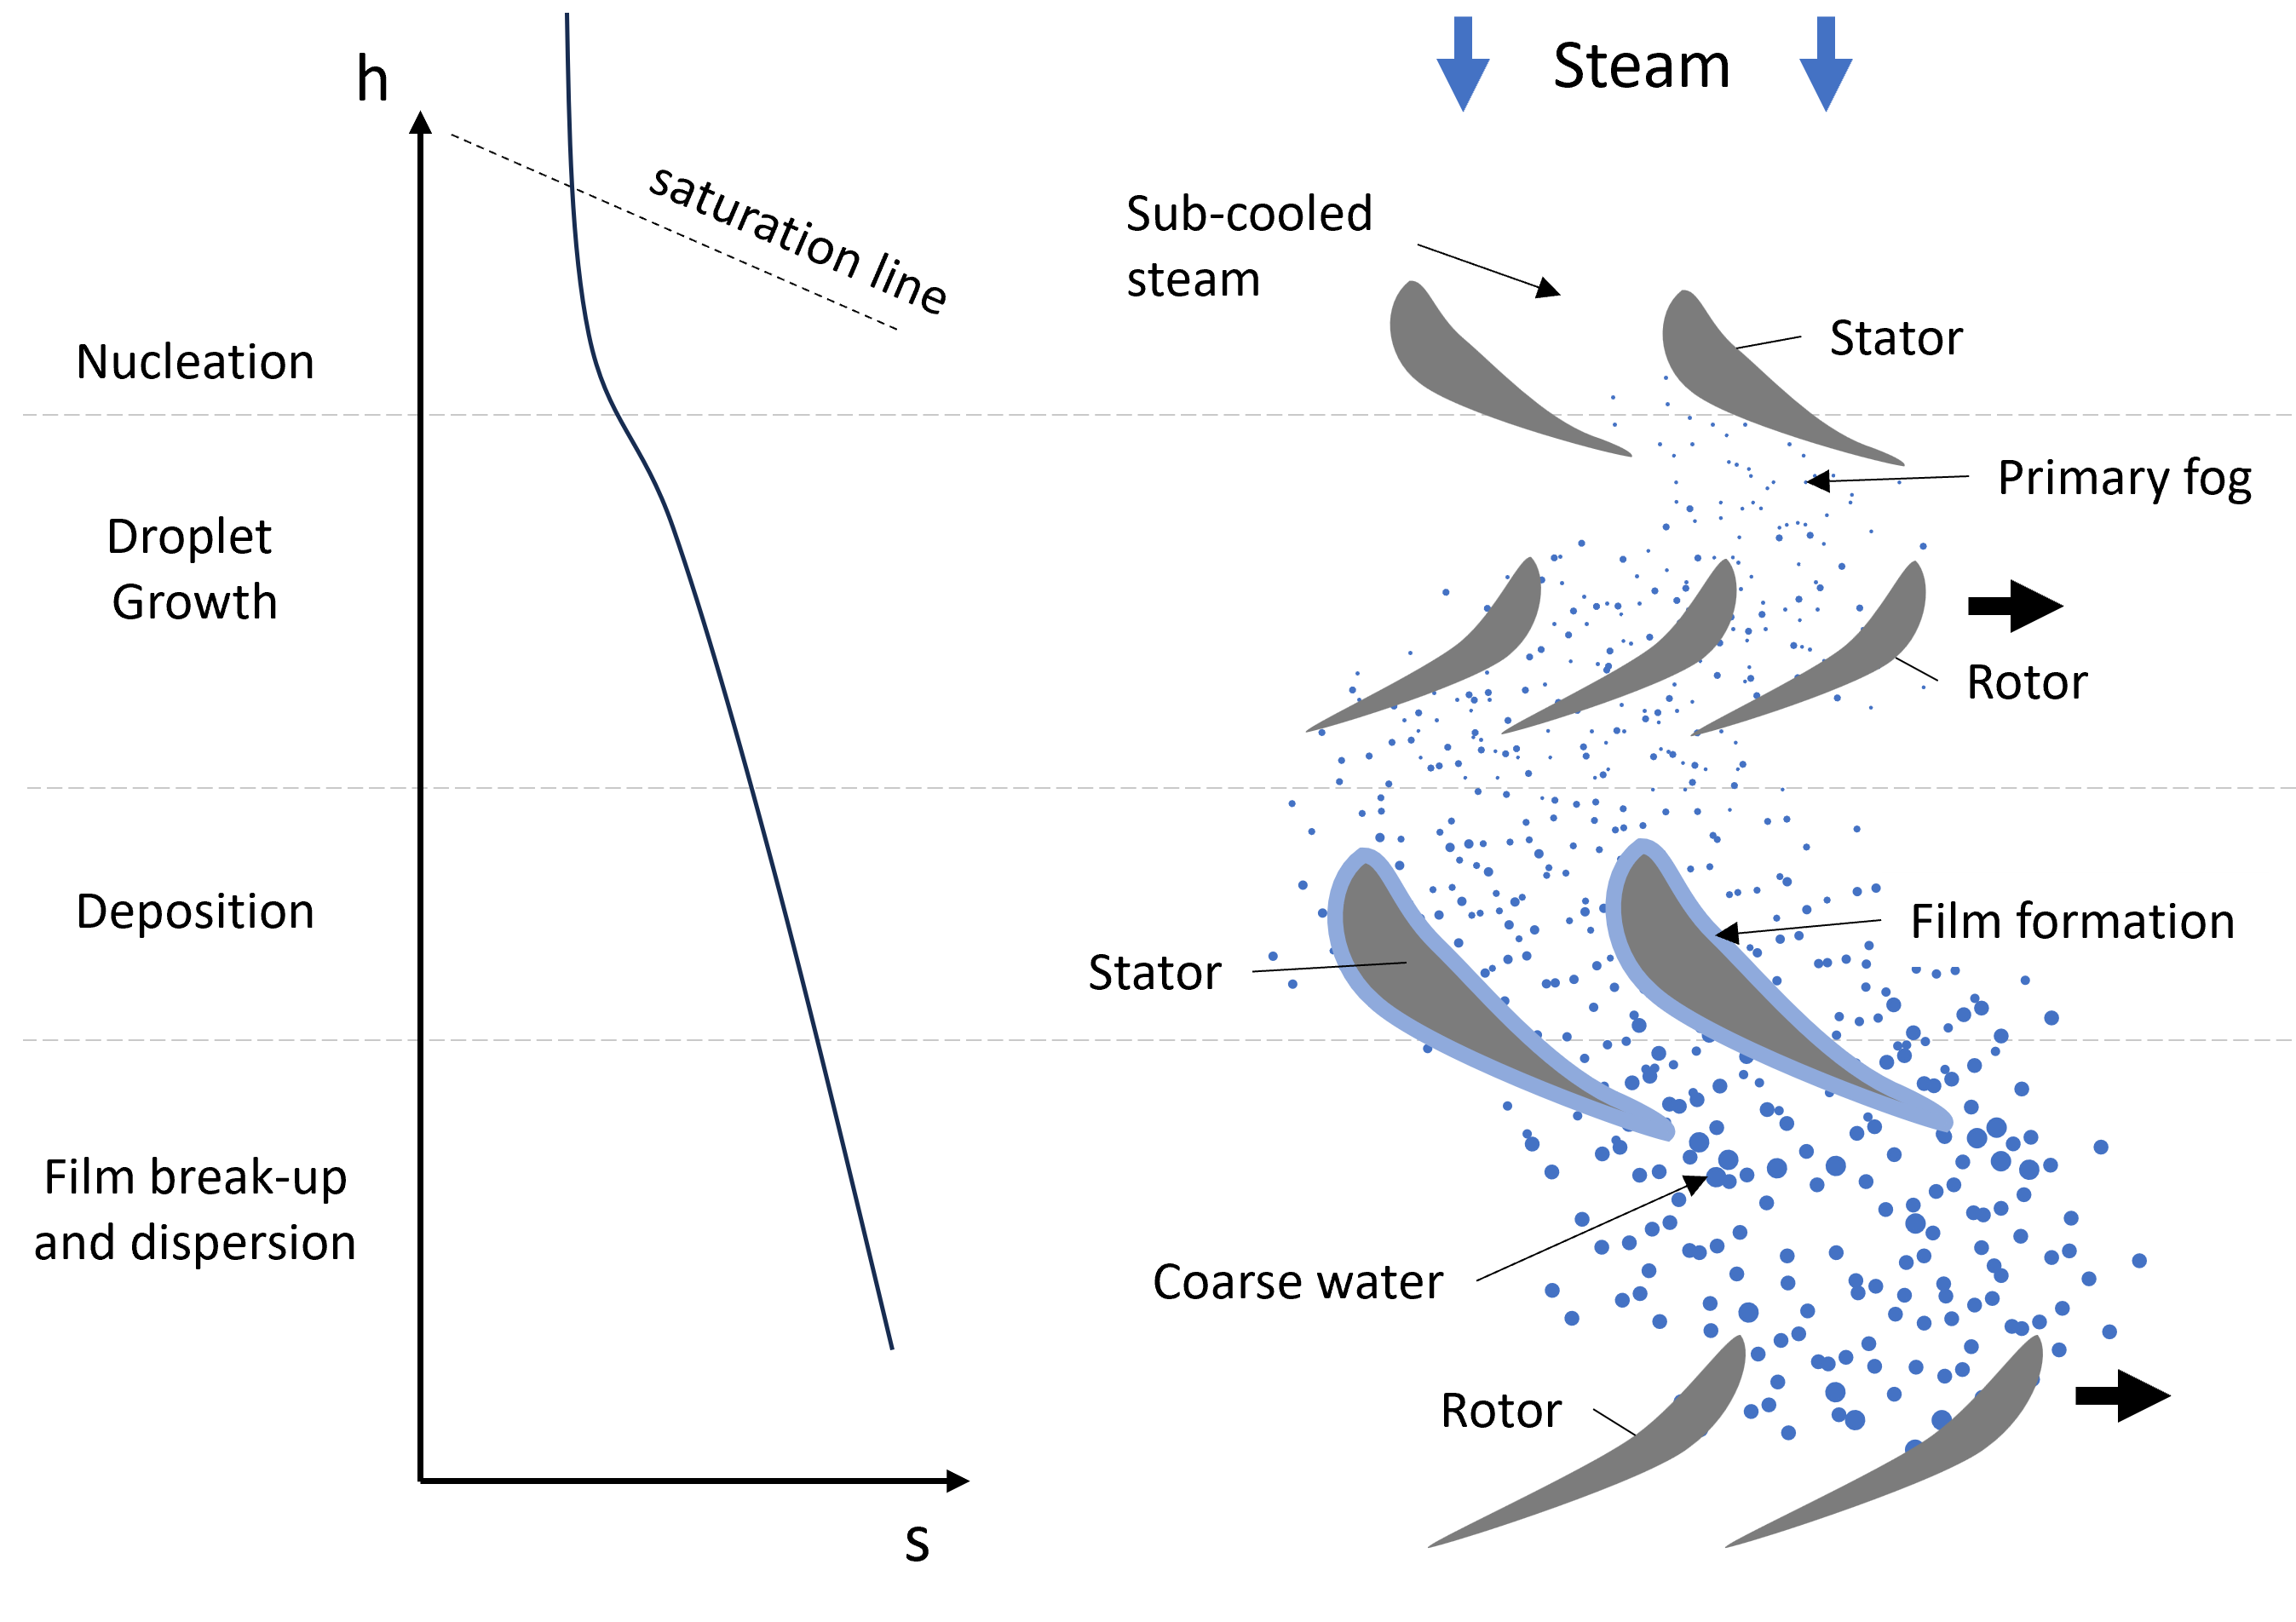
\includegraphics[width=.95\columnwidth]{Content/PowGen/Figures/Turbine/WetExpansionMechanism.png}
            \caption{Mechanism for liquid formation in a steam turbine.}
            \label{fig:prosim_litrev_WetExpansion_mech}
        \end{figure}

        The condensation of liquid is not immediate, when the fluid is initially expanded to conditions below the saturation line. The reason for this is that for a pure fluid, the only pathway from a an equilibrium vapour state to an equilibrium two-phase state is via drop-wise condensation\footnote{Droplets of condensate do not wet surfaces/sites where they form and after growing expose the condensing surface/site without forming a film \cite{Smith2005}}, due to a lack of nucleation points and wettability. However, the formation of droplets poses a thermodynamic barrier (akin to an activation energy), as it increases the surface free energy due to interactions between the droplets and the vapour. For small droplet radii, the reduction in Gibbs free energy, which is proportional to the cube of the radius, is outweighed by the change in surface free energy, which is proportional to the square of the radius \cite{McDONALD1974}. The Wilson point denotes the super-cooled conditions for which droplets are able to form spontaneously without explicit nucleation sites \cite{gyarmathy1962, McDONALD1974, Azzini2018}.

        These initial droplets, typically between \qty{0.01}{\micro\m} to \qty{1}{\micro\m}, continue to grow as the expansion progresses both due to continued condensation and coalescence with other droplets.
        
        While the difference in vapour and droplet velocity, also called slip velocity, is minimal, as the droplets grow, sharp changes in fluid velocity can result in the deposition of a small fraction of droplets on rotor or stator surfaces. Shearing with the vapour phase, gravity and centrifuging, causes the liquid to accumulate and migrate towards the trailing edge of rotor blades or nozzles, from where it is stripped of by the high velocity vapour phase. The resultant coarse droplets, \qty{10}{\micro\m} to \qty{500}{\micro\m}, are much larger than the primary fog, exhibiting higher slip velocities and therefore pressure drops, but can also have a devastating effect on the downstream turbine internals \cite{Senoo2017}.

        However, condensation also impacts the energy conversion, reducing the apparent isentropic efficiency. The main phenomena responsible for these losses are \cite{Senoo2017}:

        \begin{description}
            \item[Thermal Relaxation] Irreversible exchange of mass and heat between the vapour and the condensing droplets accounts for about \qty{60}{\percent} to \qty{90}{\percent} of losses, and is strongly droplet size dependent.
            \item[Coarse droplet \& collected Water] Coarse droplets impacting rotors and centrifuging of liquid films accounts for about \qty{10}{\percent} to \qty{40}{\percent} of losses.
            \item[Droplet Drag] Increased frictional losses due to the presence of liquid droplets, typically, account for less than \qty{5}{\percent} of losses. However, as the frictional losses depend on the slip velocity, which is small for the primary fog, higher losses can be anticipated where large or coarse droplets are more prevalent.
        \end{description}

        % \begin{itemize}
        %     \item \textbf{Thermal Relaxation}: Irreversible exchange of mass and heat between the vapour and the condensing droplets accounts for about \qty{60}{\percent} to \qty{90}{\percent} of losses, and is strongly droplet size dependent.
        %     \item \textbf{Coarse droplet \& collected Water}: Coarse droplets impacting rotors and centrifuging of liquid films accounts for about \qty{10}{\percent} to \qty{40}{\percent} of losses. 
        %     \item \textbf{Droplet Drag}: Increased frictional losses due to the presence of liquid droplets, typically, account for less than \qty{5}{\percent} of losses. However, as the frictional losses depend on the slip velocity, which is small for the primary fog, higher losses can be anticipated where large or coarse droplets are more prevalent. 
        % \end{itemize}

        Baumann \cite{Baumann1921} first proposed a rule-of-thumb for capturing the efficiency degradation due to condensation in \citeyear{Baumann1921}, see Equation~\ref{eq:litrev_Baumann}, where \(\eta_{dry, turb}\) is the isentropic efficiency corresponding to a dry expansion and \(x_{in}\) and \(x_{out}\) are the steam quality at the inlet and outlet of the turbine. Equation~\ref{eq:litrev_alternateBaumann}, is a more modern and tunable formulation of the original Baumann rule, where \(\alpha\) is the Baumann factor, typically between \num{0.4} and \num{2.5} or \num{1.0} for the original Baumann rule, and \(y_m\) is the average wetness across the turbine (sometimes weighted for dry stages) \cite{Senoo2017}.

        \begin{align}
            \eta_{isen, turb} = \eta_{dry, turb} * \frac{x_{in} + x_{out}}{2} \label{eq:litrev_Baumann}
        \end{align}
        \begin{align}
            \eta_{isen, turb} = \eta_{dry, turb} * (1-\alpha y_m) \label{eq:litrev_alternateBaumann}
        \end{align}

        However, it should be noted that the Baumann rule is entirely empirical, with the underlying source of thermodynamic losses being fluid, expansion, turbine geometry, and importantly \emph{droplet size distribution} dependent. Despite a number of analytical approaches (e.g. for predicting the droplet nucleation and growth), to accurately predict the impact of condensation on turbine performance requires sophisticated CFD simulations or experimentation\cite{Senoo2017}.


\section{Heat Exchangers}
    Heat exchangers are used to facilitate the transfer of thermal energy from one fluid stream to another. 
    
    \subsection{Working Principle}
    The rate of heat transfer \(Q\) is driven by the overall heat transfer coefficient \(U\) (the inverse of the cumulative heat transfer resistances), the area \(A\) over which the heat transfer occurs, and the difference in temperature between the two streams \(\Delta T\), Equation~\ref{eq:litrev_heatTransfer}.

    \begin{align}
        \Dot{Q} = U * A * \Delta T \label{eq:litrev_heatTransfer}
    \end{align}

    \subsubsection{Temperature Difference}
    The definition of the temperature difference depends on the heat exchange scenario. For instance, where transfer of heat does not change the temperature of either stream (e.g. exchange of latent heat), \(\Delta T\) is simply the difference in temperature between the hot and cold stream. For idealised cases of counter-current or co-current heat exchange, the log-mean temperature difference \(\Delta T_{lm}\) is used, see Equation~\ref{eq:litrev_DTlogmean}, where \(\Delta T_1\) is the difference in temperature between the two streams at the inlet of the hot stream, and \(\Delta T_2\) is the difference in temperature between the two streams at the outlet of the hot stream \cite{Smith2005}.
    
    \begin{align}
        \Delta T_{lm} = \frac{\Delta T_1 - \Delta T_2}{\ln \frac{\Delta T_1}{\Delta T_2}}\label{eq:litrev_DTlogmean}
    \end{align}   

    For real heat exchangers, where the heat transfer does not occur in a purely counter-current or co-current configuration (i.e. multiple tubing passes or shell passes in a shell and tube heat exchanger), \(\Delta T\) is obtained by applying a correction factor \(f_{T}\) to the log-mean temperature difference \(\Delta T_{lm}\), Equation~\ref{eq:litrev_DTlogmean_correction}.  

    \begin{align}
        \Delta T = f_{T}*\Delta T_{lm}\label{eq:litrev_DTlogmean_correction}
    \end{align}  

    The temperature correction factor is typically correlated based on two dimensionless numbers: the ratio of heat capacity flow rates \(R\) and thermal effectiveness of the heat exchanger \(P\), which are calculated based on the inlet and outlet temperatures of the two streams, Equations~\ref{eq:litrev_R} and \ref{eq:litrev_P} respectively. For simple geometries analytical solutions exist, for example Equation~\ref{eq:litrev_f_T_1_2} can be used to calculate the temperature correction factor for heat exchanger with one shell and two tubing passes (also referred to as a 1-2 heat exchanger). Correction factors for more complex geometries can be obtained from tables, graphical methods or simulations \cite{Smith2005}.

    \begin{align}
        R = \frac{CP^{cold}}{CP^{hot}} = \frac{\Dot{m}C_p^{cold}}{C_p^{hot}} = \frac{T_{in}^{hot} - T_{out}^{hot}}{T_{out}^{cold} - T_{in}^{cold}} \label{eq:litrev_R}
    \end{align}
    \begin{align}
        P = \frac{T_{out}^{cold} - T_{in}^{cold}}{T_{in}^{hot} - T_{in}^{cold}} \label{eq:litrev_P}
    \end{align}

    \begin{equation}
        \label{eq:litrev_f_T_1_2}
        f_T^{1-2} = \left\{
        \begin{aligned}
        \frac{\frac{\sqrt{2}P}{1-P}}{\ln\frac{2-P(2-\sqrt{2})}{2-P(2+\sqrt{2})}} \quad\quad\quad\quad\;& if\; R = 1\\
        & \\
        \frac{\sqrt{R^2+1}\ln\frac{1-P}{1-RP}}{(R-1)\ln\frac{2-P(R+1-\sqrt{R^2+1})}{2-P(R+1+\sqrt{R^2+1})}}\quad\; & if\; R \neq 1
        \end{aligned}
        \right.
    \end{equation}

    \subsubsection{Overall Heat Transfer Coefficient}
    The overall heat transfer coefficient is a measure of the ease of heat transfer between the bulk hot stream and the bulk cold stream. For a shell \& tube configuration, with the hot fluid on the shell side and the cold fluid on the tube side, the heat transfer can be broken down five stages, across the:
    
    \begin{enumerate}
        \item  \emph{Shell-side film}, Equation~\ref{eq:litrev_U_shellside}, where \(Q\) is the heat transferred, \(h_{ss}\) is the shell-side heat transfer coefficient, \(A_{ss}\) is the heat transfer area on the shell-side, and \(\Delta T_{ss}\) is the temperature difference across the shell-side fluid film.
            \begin{align}
                Q = h_{ss}A_{ss}\Delta T_{ss} \label{eq:litrev_U_shellside}
            \end{align}
        \item \emph{Shell-side fouling layer}, Equation~\ref{eq:litrev_U_shellside_fouling}, where \(Q\) is the heat transferred, \(h_{ssf}\) is the shell-side fouling layer heat transfer coefficient, \(A_{ss}\) is the heat transfer area on the shell-side, and \(\Delta T_{ssf}\) is the temperature difference across the shell-side fouling film. Fouling (i.e. the deposition of materials on surfaces, such as scales, biofilms, etc.) is a time dependent phenomenon, with complex mechanisms and multi variable dependencies, as such for design is usually performed with experienced based values of fouling resistance after a reasonable period of operation \cite{Smith2005}.     
            \begin{align}
                Q = h_{ssf}A_{ss}\Delta T_{ssf} \label{eq:litrev_U_shellside_fouling}
            \end{align}
        \item \emph{Tubing}, Equation~\ref{eq:litrev_U_tubing}, where \(Q\) is the heat transferred, \(k\) is the thermal conductivity of the tubing material, \(L\) is the length of the tubing, \(\Delta T_{tw}\) is the temperature difference across the tubing wall, and \(d_{ss}\) and \(d_{ts}\) are the tubing diameter on the shell and tubing side respectively.
            \begin{align}
                Q = \frac{2\pi kL}{\ln \frac{d_{ss}}{d_{ts}}}\Delta T_{tw} \label{eq:litrev_U_tubing}
            \end{align}
        \item \emph{Tube-side fouling layer}, Equation~\ref{eq:litrev_U_tubeside_fouling}, where \(Q\) is the heat transferred, \(h_{tsf}\) is the tube-side heat transfer coefficient, \(A_{ts}\) is the heat transfer area on the tube-side, and \(\Delta T_{tsf}\) is the temperature difference across the tube-side fluid film.
            \begin{align}
                Q = h_{tsf}A_{ts}\Delta T_{tsf} \label{eq:litrev_U_tubeside_fouling}
            \end{align}
        \item \emph{Tube-side film}, Equation~\ref{eq:litrev_U_tubeside}, where \(Q\) is the heat transferred, \(h_{ts}\) is the tube-side heat transfer coefficient, \(A_{ts}\) is the heat transfer area on the tube-side, and \(\Delta T_{ts}\) is the temperature difference across the tube-side fluid film.
            \begin{align}
                Q = h_{ts}A_{ts}\Delta T_{ts} \label{eq:litrev_U_tubeside}
            \end{align}
    \end{enumerate}

    Combining Equations~\ref{eq:litrev_U_shellside} to ~\ref{eq:litrev_U_tubeside}, an expression for the overall heat transfer coefficient \(U\) can be obtained, Equation~\ref{eq:litrev_U_overall} ( \emph{Note}, this formulation is relative to the shell-side heat transfer area).

    \begin{align}
        U = \left[\frac{1}{h_{ss}} + \frac{1}{h_{ssf}}+ \frac{d_{ss}\ln \frac{d_{ss}}{d_{ts}}}{2\pi kL} + \frac{d_{ss}}{h_{tsf}d_{ts}} + \frac{d_{ss}}{h_{ts}d_{ts}}\right]^{-1} \label{eq:litrev_U_overall}
    \end{align}

    An alternative, more generic formulation of the overall heat transfer coefficient \(U\) is given by Equation~\ref{eq:litrev_U_overall_general}.

    \begin{align}
        U = \left[\frac{1}{h_{int}\chi_{int}\frac{A_{int,\;pt}}{A_{ext,\;pt}}} +  \frac{R_{int,\;f}}{\frac{A_{int,\;pt}}{A_{ext,\;pt}}} + R_{m} + \frac{R_{ext,\;f}}{\frac{A_{ext,\;t}}{A_{ext,\;pt}}} + \frac{1}{h_{ext}\chi_{ext}\frac{A_{ext,\;t}}{A_{ext,\;pt}}}\right]^{-1} \label{eq:litrev_U_overall_general}
    \end{align}

    Here,
    \begin{itemize}
        \item \(h_{int}\) and \(h_{ext}\) are the internal and external film heat transfer coefficients. Exact values are not usually known until detailed design calculations have been performed. \citeauthor{Astolfi2014C} \cite{Astolfi2014C} obtained typical values by performing regression analysis against overall heat transfer coefficient data, see Table~\ref{table:FilmHeatTransferCoefficient}.
        \item \(\chi_{int}\) and \(\chi_{ext}\) are the internal and external enhancement factor, with typical values ranging from 1 to 5. The enhancement factor accounts for improvement of the film heat transfer from turbulence/mixing promoting texturing of the heat transfer surface.  
        \item \(\frac{A_{int,\;pt}}{A_{ext,\;pt}}\) is the ratio of the internal to the external \emph{plain} tubing area. It is usually around \num{0.87}.
        \item \(\frac{A_{ext,\;t}}{A_{ext,\;pt}}\) is the ratio of the external heat transfer area to the external plain tubing area. For plain tubes its value is \num{1}, however for finned tubes its value can be as large as \num{14}.
        \item \(R_{int,\;f}\) and \(R_{ext,\;f}\) are the heat transfer resistances the internal and external fouling layer. Typical values are shown in Table~\ref{table:FoulingResistances}
        \item \(R_{m}\) is the resistance of the material. Due to the high thermal conductivity of the materials used, the material resistance is small and can be neglected. 
    \end{itemize}

    \begin{table}[H]
        \caption{Film heat transfer coefficients for different fluids \cite{Astolfi2014C}.}
        \centering 
        \label{table:FilmHeatTransferCoefficient}
        \begin{tabular}{|c c |}
    \hline
    \rowcolor{bluepoli!40} % comment this line to remove the color
    \textbf{Fluid} & \(\mathbf{h}\)/\unit{\watt\per\m\squared\per\K} \T\B \\
    \hline \hline
    Water (liquid) & 7500 \T\B \\
    Water (boiling)& 7000 \T\B \\
    Water (condensing)& 10000 \T\B \\
    Water (vapour LP)& 125 \T\B \\
    Water (vapour HP)& 800\T\B \\
    \hline
    Organic (liquid) & 1900 \T\B \\
    Organic (boiling)& 1900 \T\B \\
    Organic (condensing)& 2500 \T\B \\
    Organic (vapour LP)& 125 \T\B \\
    Organic (vapour HP)& 600\T\B \\
    \hline
    Air & 125 \T\B \\

    \hline
\end{tabular}
        \\[10pt]
    \end{table}

    \begin{table}[H]
        \caption[Fouling resistances for different fluids.]{Fouling resistances for different fluids \cite{TEMA2019}. \textsuperscript{a}Sodium Chloride or Calcium Chloride solutions in TEMA standard \textsuperscript{b} Refrigerant in TEMA standard}
        \centering 
        \label{table:FoulingResistances}
        \begin{tabular}{|c c |}
    \hline
    \rowcolor{bluepoli!40} % comment this line to remove the color
    \textbf{Fluid} & \(\mathbf{R_f}\)/\qty{e-5}{\square\m\K\per\watt} \T\B \\
    \hline \hline
    Steam & 8.81 \T\B \\
    Water & 8.81 \T\B \\
    Brine\textsuperscript{a} & 52.83 \T\B \\
    Organic\textsuperscript{b} (vapour) & 35.22 \T\B \\
    Organic\textsuperscript{b} (liquid) & 17.61 \T\B \\
    Air & 17.61 \T\B \\

    \hline
\end{tabular}
        \\[10pt]
    \end{table}

    \subsection{Shell \& Tube Heat Exchangers}
        In shell and tube heat exchangers, one fluid flow through a collection of tubes, which are contained within an outer shell. The other fluid flows through the interspace between the tubes and the shell, Figure~\ref{fig:prosim_litrev_ShellandTubeHX}. On the shell side, baffles are used not only to hold tubes in place and reduce vibrations, but also to ensure even flow across all tubes and prevent short-circuiting \cite{Incropera2007}.

        \begin{figure}[H]
            \centering
            \includesvg[width=0.8\columnwidth]{Content/PowGen/Figures/Shell_and_Tube_HX.svg}
            \caption[Shell \& Tube heat exchanger.]{Shell \& Tube heat exchanger. Adapted from \cite{Incropera2007}}
            \label{fig:prosim_litrev_ShellandTubeHX}
        \end{figure}

        Shell and tube heat exchangers can be divided into three core components, 1) the front end, 2) the shell and 3) the rear end, with many possible configurations being available for each component \cite{TEMA2019}. This versatility has made shell and tube heat exchangers popular across many industries, with \ac{TEMA} providing standards for their design and operation since as early as 1939 \cite{TEMA2024}. 

        For \emph{dirty} fluids, such as scaling-prone geofluids, \ac{TEMA} recommend confining the fluid to the tube-side reduce maintenance costs (compared to the shell-side), and to avoid U-bends, as these may make it impossible to clean the U-bend section of the tubing, which may lead to high pressure losses and in the worst case clogging.

        % \textbf{Parallel Plate}\\
        %     In parallel plate heat exchangers, the fluids both flow between parallel plates stacked together. Their modular design makes them well suited for low-cost maintenance, and also them to be extended to increase capacity, if so required. Parallel plate heat exchangers offer some of the highest heat transfer surface area to volume ratios, allowing very low approach temperatures to be achieved \cite{Incropera2007}.

        %     % \begin{figure}[H]
        %     %     \centering
        %     %     \includesvg[width=0.8\columnwidth]{Content/PowGen/Figures/Shell_and_Tube_HX.svg}
        %     %     \caption[Parallel plate heat exchanger.]{Parallel plate heat exchanger. Adapted from \cite{Incropera2007}}
        %     %     \label{fig:prosim_litrev_ParallelPlateHX}
        %     % \end{figure}
        %     % \todo{draw parallel plate HX}

        %     However, parallel plate heat exchangers are not well suited to high pressure applications, as unlike tubes, large flat surfaces are not ideal for containing pressures. Moreover, the typical rubber gaskets are not designed to withstand the high temperatures encountered in a geothermal setting. To prevent leakage for fluids (e.g. ORC working fluid into the geofluid or the atmosphere; or geofluid into the ORC working fluid), it is possible for the parallel plates to be welded together, avoiding the need for gaskets, but this results them no longer being disassemble for maintenance \cite{Incropera2007}.

        %     \todo{probably not useful in ORC or DSC applications, but perhaps the welded ones could be used in low fouling applications... perhaps for the recuperator??}

        % \textbf{Air Coolers}\\
        %     - low heat capacity -> high mass rate -> high fan power
        %     - low air heat transfer coefficient -> use of fins and corrugated surface
        %     - humid air?

        % \textbf{Cooling Tower}\\
        %     - direct contact heat exchanger
        %         * air flows past water, evaporating some in the process -> evaporation carries away heat, cooling the remaining liquid.
        %         * for large capacity use natural draft, low capacity use mechanical draft (Walraven)
        %         * 


        % \todo{What configuration is best suited for what application}

\section{Equipment Costs}

    \subsection{Steam Turbines}
        Steam turbines have not only been installed in many power plants across the globe but also for many decades, yielding significant experience in their design, manufacture and operation. Some cost correlations, in terms of the fluid power \(\Dot{W}\), i.e. work done by the fluid, (or similar) are shown in Table~\ref{table:SteamTurbineCosts}.

        The \emph{genGEO} steam turbine cost model suggested by \citeauthor{Adams2021} \cite{Adams2021} is a development of a cost model from \emph{GETEM} \cite{GETEM2016}, where the specific cost has been matched against cost data of coal-fired power stations reported by \ac{NETL} between 2007 and 2019. This also explains the similarity in specific cost predicted by either model, see Figure~ \ref{fig:prosim_litrev_steamturb_speccost}.
        
        \begin{table}[H]
            \caption[Steam turbine cost correlations.]{Steam turbine cost correlations.\(\Dot{W}\) is the fluid power in \unit{\kilo\watt}, \(\Dot{W}_s\) is the shaft power in \unit{\kilo\watt}, and \(\Dot{W}_e\) is the electrical power in \unit{\kilo\watt}. \textsuperscript{a}Fitted against data from Thermoflex, \(R^2=0.9994\)}
            \centering 
            \label{table:SteamTurbineCosts}
            \scalebox{0.75}{
                \begin{tabular}{|c | c c | c | c |}
    \hline
    \rowcolor{bluepoli!40} % comment this line to remove the color
    \textbf{Cost Correlation} & \textbf{Min}/\unit{\kilo\watt} & \textbf{Max}/\unit{\kilo\watt} & \textbf{Currency} & \textbf{Reference} \T\B \\
    \hline \hline
        \(C_{turb,\; gen} = 2830\cdot \Dot{W}_e^{0.745} + 3685\cdot \Dot{W}_e^{0.617}\) & - & - & \euro2002 &\cite{GETEM2016} \T\B \\
    \(C_{turb,\; gen} = 0.67 \cdot(2830 \cdot \Dot{W}^{0.745} + 3680\cdot \Dot{W}^{0.617}\) & - & - & \euro2002 &\cite{Adams2021} \T\B \\
    \(\log C_{turb,\; gen} = 2.6259 + 1.4398\log \Dot{W}_s -0.1776(\log \Dot{W}_s)^2\) & 70 & 7500& \euro2001 &\cite{Turton2012} \T\B \\
    \(C_{turb,\; gen} = 10^3\cdot\exp \left(-0.0408\ln^2\Dot{W}_e + 1.3039\ln^2\Dot{W}_e -0.1583\right)\) & 500 & 70000 & \euro2021 &\cite{Thermoflex2021}\textsuperscript{a} \T\B \\
    \hline
\end{tabular}
            }
            % \\[6pt]
        \end{table}

        However, although steam turbines share the same working fluid, there are some stark differences in the expansion processes used in coal-fired and geothermal power stations. As discussed in Section~\ref{sec:prosim_litrev_wet_expansion}, wet expansion is unavoidable in geothermal \ac{DSC} power plants and reduces the isentropic efficiency of the turbine. In turn, this should lead to higher specific costs for geothermal steam turbines.

        With this in mind, a wet expansion turbine was simulated in \emph{Thermoflex} \cite{Thermoflex2021} for a range of operating conditions, analogous to a geothermal \ac{DSC} and different mass rates. The combined turbine and generator costs predicted by \emph{Thermoflex} were then correlated against the turbine power. 

        % \begin{figure}[H]
        %     \centering
        %     % This file was created with tikzplotlib v0.10.1.
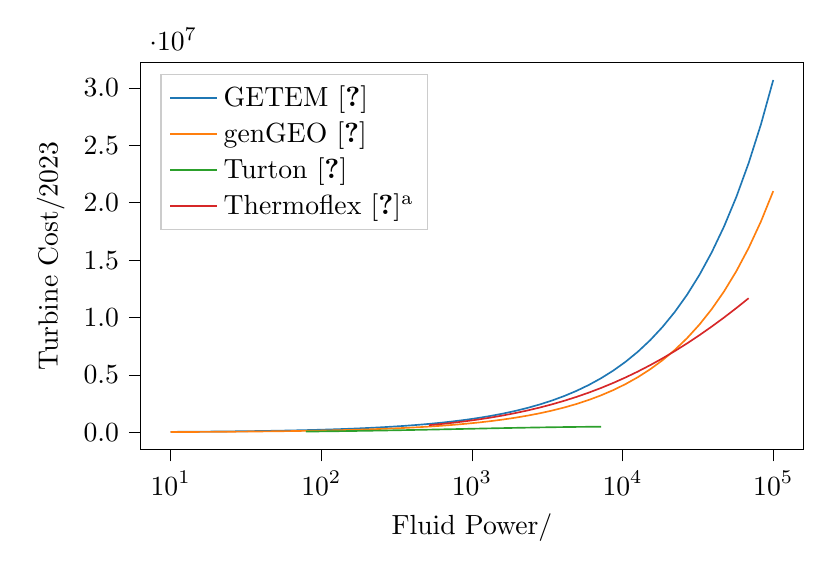
\begin{tikzpicture}

\definecolor{crimson2143940}{RGB}{214,39,40}
\definecolor{darkgray176}{RGB}{176,176,176}
\definecolor{darkorange25512714}{RGB}{255,127,14}
\definecolor{forestgreen4416044}{RGB}{44,160,44}
\definecolor{lightgray204}{RGB}{204,204,204}
\definecolor{steelblue31119180}{RGB}{31,119,180}

\begin{axis}[
legend cell align={left},
legend style={
  fill opacity=0.8,
  draw opacity=1,
  text opacity=1,
  at={(0.03,0.97)},
  anchor=north west,
  draw=lightgray204
},
log basis x={10},
tick align=outside,
tick pos=left,
unbounded coords=jump,
x grid style={darkgray176},
xlabel={Fluid Power/\unit{\kilo\watt}},
xmin=6.30957344480193, xmax=158489.319246111,
xmode=log,
xtick style={color=black},
xtick={0.1,1,10,100,1000,10000,100000,1000000,10000000},
xticklabels={
  \(\displaystyle {10^{-1}}\),
  \(\displaystyle {10^{0}}\),
  \(\displaystyle {10^{1}}\),
  \(\displaystyle {10^{2}}\),
  \(\displaystyle {10^{3}}\),
  \(\displaystyle {10^{4}}\),
  \(\displaystyle {10^{5}}\),
  \(\displaystyle {10^{6}}\),
  \(\displaystyle {10^{7}}\)
},
y grid style={darkgray176},
ylabel={Turbine Cost/\unit{\USD}2023},
ymin=-1499646.00511472, ymax=32227165.3666998,
ytick style={color=black},
ytick={-5000000,0,5000000,10000000,15000000,20000000,25000000,30000000,35000000},
yticklabels={\ensuremath{-}0.5,0.0,0.5,1.0,1.5,2.0,2.5,3.0,3.5},
width=10cm, height=6.5cm
]
\addplot [semithick, steelblue31119180]
table {%
10 48812.6480559191
12.0679264063933 55491.4054284559
14.5634847750124 63093.1030820432
17.5751062485479 71746.5150730635
21.2095088792019 81598.5476326557
25.5954792269954 92816.8141278817
30.8884359647748 105592.578561663
37.2759372031494 120144.120731392
44.9843266896944 136720.583870834
54.2867543932386 155606.374428351
65.5128556859551 177126.193751249
79.060432109077 201650.793040153
95.4095476349994 229603.556225333
115.139539932645 261468.030647655
138.949549437314 297796.542885418
167.683293681101 339220.057082189
202.358964772516 386459.456075458
244.205309454865 440338.451932414
294.705170255181 501798.362662221
355.648030622313 571915.026461224
429.193426012878 651918.164510367
517.947467923121 743213.548830249
625.055192527397 847408.383867207
754.312006335462 966340.370318703
910.298177991522 1102110.98833917
1098.54114198756 1257123.61599665
1325.71136559011 1434127.18916655
1599.85871960606 1636266.21266305
1930.69772888325 1867138.0512855
2329.95181051537 2130858.56585319
2811.76869797423 2432137.31580617
3393.22177189533 2776363.72953824
4094.91506238042 3169705.8497147
4941.71336132383 3619223.49733526
5963.62331659464 4132997.96973533
7196.85673001151 4720280.69924962
8685.11373751352 5391663.65683186
10481.1313415469 6159274.69535598
12648.552168553 7037001.49845596
15264.1796717523 8040748.34159303
18420.6996932672 9188730.49291243
22229.9648252619 10501811.7942418
26826.9579527973 12003891.7809356
32374.5754281764 13722349.6388555
39069.3993705461 15688553.3755993
47148.6636345739 17938443.8218413
56898.6602901829 20513204.5010771
68664.88450043 23460030.0394899
82864.2772854684 26833007.663429
100000 30694128.4861628
};
\addlegendentry{GETEM \cite{GETEM2016}}
\addplot [semithick, darkorange25512714]
table {%
10 33390.8754223091
12.0679264063933 37960.4490544543
14.5634847750124 43161.6141882102
17.5751062485479 49082.5102628811
21.2095088792019 55823.6894198832
25.5954792269954 63499.8795177257
30.8884359647748 72241.99951316
37.2759372031494 82199.4635883837
44.9843266896944 93542.8156814665
54.2867543932386 106466.742124188
65.5128556859551 121193.517021064
79.060432109077 137976.942944889
95.4095476349994 157106.85862615
115.139539932645 178914.295746414
138.949549437314 203777.378904844
167.683293681101 232128.076536456
202.358964772516 264459.926278003
244.205309454865 301336.876297774
294.705170255181 343403.404767905
355.648030622313 391396.103351025
429.193426012878 446156.93774356
517.947467923121 508648.429478027
625.055192527397 579971.038924406
754.312006335462 661383.070421006
910.298177991522 754323.467483235
1098.54114198756 860437.919973758
1325.71136559011 981608.766991027
1599.85871960606 1119989.25021756
1930.69772888325 1278042.7539108
2329.95181051537 1458587.76116363
2811.76869797423 1664849.36328337
3393.22177189533 1900518.2821753
4094.91506238042 2169818.50680974
4941.71336132383 2477584.8068877
5963.62331659464 2829351.57278575
7196.85673001151 3231454.64429991
8685.11373751352 3691148.03569228
10481.1313415469 4216737.74574811
12648.552168553 4817735.16434458
15264.1796717523 5505032.95758494
18420.6996932672 6291106.73894627
22229.9648252619 7190246.32226551
26826.9579527973 8218820.91309568
32374.5754281764 9395583.23873954
39069.3993705461 10742018.3564526
47148.6636345739 12282743.7280706
56898.6602901829 14045968.1239458
68664.88450043 16064018.0382776
82864.2772854684 18373941.583189
100000 21018201.3049328
};
\addlegendentry{genGEO \cite{Adams2021}}
\addplot [semithick, forestgreen4416044]
table {%
10 nan
12.0679264063933 nan
14.5634847750124 nan
17.5751062485479 nan
21.2095088792019 nan
25.5954792269954 nan
30.8884359647748 nan
37.2759372031494 nan
44.9843266896944 nan
54.2867543932386 nan
65.5128556859551 nan
79.060432109077 75757.2960227814
95.4095476349994 87245.4089363145
115.139539932645 99929.4935354662
138.949549437314 113835.514898739
167.683293681101 128971.82713424
202.358964772516 145326.533700989
244.205309454865 162865.075032369
294.705170255181 181528.157113581
355.648030622313 201230.135637579
429.193426012878 221857.966192864
517.947467923121 243270.821203174
625.055192527397 265300.458892425
754.312006335462 287752.408545953
910.298177991522 310408.010271511
1098.54114198756 333027.317158292
1325.71136559011 355352.834336197
1599.85871960606 377114.034375044
1930.69772888325 398032.553372438
2329.95181051537 417827.938727689
2811.76869797423 436223.789786279
3393.22177189533 452954.107986839
4094.91506238042 467769.655384144
4941.71336132383 480444.110699502
5963.62331659464 490779.811222727
7196.85673001151 498612.87736368
8685.11373751352 nan
10481.1313415469 nan
12648.552168553 nan
15264.1796717523 nan
18420.6996932672 nan
22229.9648252619 nan
26826.9579527973 nan
32374.5754281764 nan
39069.3993705461 nan
47148.6636345739 nan
56898.6602901829 nan
68664.88450043 nan
82864.2772854684 nan
100000 nan
};
\addlegendentry{Turton \cite{Turton2012}}
\addplot [semithick, crimson2143940]
table {%
10 nan
12.0679264063933 nan
14.5634847750124 nan
17.5751062485479 nan
21.2095088792019 nan
25.5954792269954 nan
30.8884359647748 nan
37.2759372031494 nan
44.9843266896944 nan
54.2867543932386 nan
65.5128556859551 nan
79.060432109077 nan
95.4095476349994 nan
115.139539932645 nan
138.949549437314 nan
167.683293681101 nan
202.358964772516 nan
244.205309454865 nan
294.705170255181 nan
355.648030622313 nan
429.193426012878 nan
517.947467923121 631939.931792051
625.055192527397 732928.578359439
754.312006335462 847608.744485545
910.298177991522 977410.761578113
1098.54114198756 1123845.78149899
1325.71136559011 1288499.45283318
1599.85871960606 1473023.49031962
1930.69772888325 1679124.97828581
2329.95181051537 1908553.27424805
2811.76869797423 2163084.4111542
3393.22177189533 2444502.93617475
4094.91506238042 2754581.17040562
4941.71336132383 3095055.92702202
5963.62331659464 3467602.78475733
7196.85673001151 3873808.07825212
8685.11373751352 4315138.83573619
10481.1313415469 4792910.9663104
12648.552168553 5308256.0721726
15264.1796717523 5862087.33363609
18420.6996932672 6455064.98467515
22229.9648252619 7087561.96180169
26826.9579527973 7759630.36703663
32374.5754281764 8470969.43426095
39069.3993705461 9220895.72503231
47148.6636345739 10008316.3028706
56898.6602901829 10831705.6420964
68664.88450043 11689087.0168826
82864.2772854684 nan
100000 nan
};
\addlegendentry{Thermoflex \cite{Thermoflex2021}\textsuperscript{a}}
\end{axis}

\end{tikzpicture}

        %     \caption[Steam turbine cost correlations.]{Steam turbine cost correlations. \textsuperscript{a}Fitted against data from Thermoflex, \(R^2=0.9994\)}
        %     \label{fig:prosim_litrev_steamturb_cost}
        % \end{figure}

        \begin{figure}[H]
            \centering
            % This file was created with tikzplotlib v0.10.1.
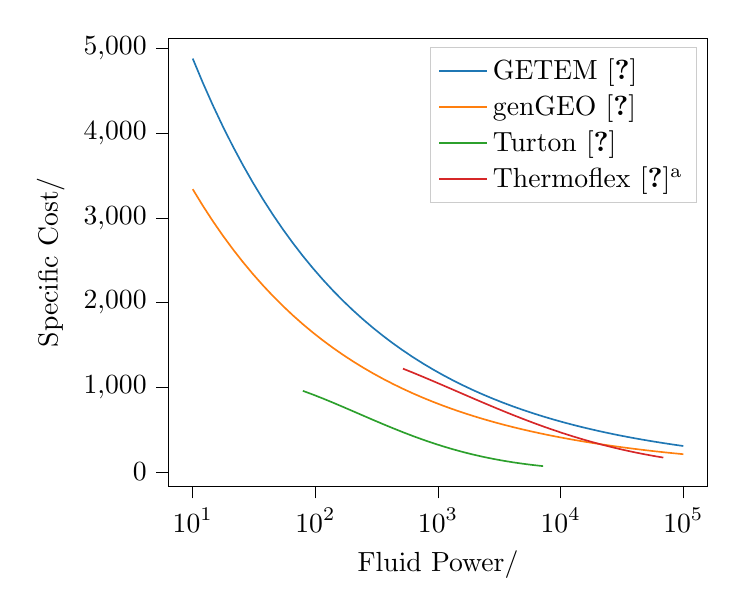
\begin{tikzpicture}

\definecolor{crimson2143940}{RGB}{214,39,40}
\definecolor{darkgray176}{RGB}{176,176,176}
\definecolor{darkorange25512714}{RGB}{255,127,14}
\definecolor{forestgreen4416044}{RGB}{44,160,44}
\definecolor{lightgray204}{RGB}{204,204,204}
\definecolor{steelblue31119180}{RGB}{31,119,180}

\begin{axis}[
legend cell align={left},
legend style={fill opacity=0.8, draw opacity=1, text opacity=1, draw=lightgray204},
log basis x={10},
tick align=outside,
tick pos=left,
unbounded coords=jump,
x grid style={darkgray176},
xlabel={Fluid Power/\unit{\kilo\watt}},
xmin=6.30957344480193, xmax=158489.319246111,
xmode=log,
xtick style={color=black},
xtick={0.1,1,10,100,1000,10000,100000,1000000,10000000},
xticklabels={
  \(\displaystyle {10^{-1}}\),
  \(\displaystyle {10^{0}}\),
  \(\displaystyle {10^{1}}\),
  \(\displaystyle {10^{2}}\),
  \(\displaystyle {10^{3}}\),
  \(\displaystyle {10^{4}}\),
  \(\displaystyle {10^{5}}\),
  \(\displaystyle {10^{6}}\),
  \(\displaystyle {10^{7}}\)
},
y grid style={darkgray176},
ylabel={Specific Cost/\unit{\USD\per\kilo\watt}},
ymin=-171.317103893603, ymax=5121.86394413884,
ytick style={color=black}
]
\addplot [semithick, steelblue31119180]
table {%
10 4881.26480559191
12.0679264063933 4598.25520638391
14.5634847750124 4332.28063590222
17.5751062485479 4082.28058814673
21.2095088792019 3847.26247540184
25.5954792269954 3626.29717946396
30.8884359647748 3418.5148993002
37.2759372031494 3223.10127513685
44.9843266896944 3039.29377033792
54.2867543932386 2866.37829370273
65.5128556859551 2703.68604599268
79.060432109077 2550.59057559845
95.4095476349994 2406.50502928395
115.139539932645 2270.87958489856
138.949549437314 2143.19905383908
167.683293681101 2022.98064187191
202.358964772516 1909.77185769803
244.205309454865 1803.14855936332
294.705170255181 1702.71312928688
355.648030622313 1608.09276930477
429.193426012878 1518.93790770879
517.947467923121 1434.92071080182
625.055192527397 1355.73369199723
754.312006335462 1281.08841196006
910.298177991522 1210.71426372715
1098.54114198756 1144.35733715186
1325.71136559011 1081.77935740046
1599.85871960606 1022.75669258218
1930.69772888325 967.079425926236
2329.95181051537 914.550488227418
2811.76869797423 864.984846569503
3393.22177189533 818.208745603877
4094.91506238042 774.058997910475
4941.71336132383 732.382320201128
5963.62331659464 693.034712342522
7196.85673001151 655.880876378384
8685.11373751352 620.793672919181
10481.1313415469 587.653612443613
12648.552168553 556.34837922015
15264.1796717523 526.772385709868
18420.6996932672 498.826355454399
22229.9648252619 472.416932585858
26826.9579527973 447.456316219558
32374.5754281764 423.86191810604
39069.3993705461 401.556042026761
47148.6636345739 380.465583518408
56898.6602901829 360.521748604622
68664.88450043 341.659790301446
82864.2772854684 323.818761744449
100000 306.941284861628
};
\addlegendentry{GETEM \cite{GETEM2016}}
\addplot [semithick, darkorange25512714]
table {%
10 3339.08754223091
12.0679264063933 3145.5651763292
14.5634847750124 2963.68725308557
17.5751062485479 2792.72907763709
21.2095088792019 2632.012355299
25.5954792269954 2480.90215285959
30.8884359647748 2338.80406232108
37.2759372031494 2205.16155342806
44.9843266896944 2079.45350225496
54.2867543932386 1961.19188399019
65.5128556859551 1849.91961886109
79.060432109077 1745.20856089589
95.4095476349994 1646.65761991851
115.139539932645 1553.89100782473
138.949549437314 1466.55660079544
167.683293681101 1384.32440966907
202.358964772516 1306.88515122272
244.205309454865 1233.94891360242
294.705170255181 1165.24390960144
355.648030622313 1100.5153119115
429.193426012878 1039.5241648696
517.947467923121 982.046367593259
625.055192527397 927.871723742196
754.312006335462 876.803053466012
910.298177991522 828.655363397048
1098.54114198756 783.255070826927
1325.71136559011 740.439278465481
1599.85871960606 700.055096423353
1930.69772888325 661.95900828559
2329.95181051537 626.01627835427
2811.76869797423 592.100397334542
3393.22177189533 560.092563921558
4094.91506238042 529.881199916367
4941.71336132383 501.361496657909
5963.62331659464 474.434990706518
7196.85673001151 449.009166852587
8685.11373751352 424.997086652895
10481.1313415469 402.317040817254
12648.552168553 380.892223880177
15264.1796717523 360.65042969669
18420.6996932672 341.523766398824
22229.9648252619 323.448389540166
26826.9579527973 306.364252240485
32374.5754281764 290.214871221518
39069.3993705461 274.947107698586
47148.6636345739 260.510962161475
56898.6602901829 246.859382142065
68664.88450043 233.948082125981
82864.2772854684 221.735374821294
100000 210.182013049328
};
\addlegendentry{genGEO \cite{Adams2021}}
\addplot [semithick, forestgreen4416044]
table {%
10 nan
12.0679264063933 nan
14.5634847750124 nan
17.5751062485479 nan
21.2095088792019 nan
25.5954792269954 nan
30.8884359647748 nan
37.2759372031494 nan
44.9843266896944 nan
54.2867543932386 nan
65.5128556859551 nan
79.060432109077 958.22011089266
95.4095476349994 914.430590008479
115.139539932645 867.899017087647
138.949549437314 819.257891513317
167.683293681101 769.13939548157
202.358964772516 718.162073345058
244.205309454865 666.918648885764
294.705170255181 615.965294929838
355.648030622313 565.812596474853
429.193426012878 516.918370008321
517.947467923121 469.682422000531
625.055192527397 424.443252474535
754.312006335462 381.476638485299
910.298177991522 340.995970085751
1098.54114198756 303.154160030598
1325.71136559011 268.04690942513
1599.85871960606 235.717085361077
1930.69772888325 206.159953170229
2329.95181051537 179.329004506436
2811.76869797423 155.142131748092
3393.22177189533 133.487917512045
4094.91506238042 114.23183344668
4941.71336132383 97.2221728722031
5963.62331659464 82.2955752180158
7196.85673001151 69.282034653326
8685.11373751352 nan
10481.1313415469 nan
12648.552168553 nan
15264.1796717523 nan
18420.6996932672 nan
22229.9648252619 nan
26826.9579527973 nan
32374.5754281764 nan
39069.3993705461 nan
47148.6636345739 nan
56898.6602901829 nan
68664.88450043 nan
82864.2772854684 nan
100000 nan
};
\addlegendentry{Turton \cite{Turton2012}}
\addplot [semithick, crimson2143940]
table {%
10 nan
12.0679264063933 nan
14.5634847750124 nan
17.5751062485479 nan
21.2095088792019 nan
25.5954792269954 nan
30.8884359647748 nan
37.2759372031494 nan
44.9843266896944 nan
54.2867543932386 nan
65.5128556859551 nan
79.060432109077 nan
95.4095476349994 nan
115.139539932645 nan
138.949549437314 nan
167.683293681101 nan
202.358964772516 nan
244.205309454865 nan
294.705170255181 nan
355.648030622313 nan
429.193426012878 nan
517.947467923121 1220.08499110155
625.055192527397 1172.58217693682
754.312006335462 1123.68454613805
910.298177991522 1073.72593421495
1098.54114198756 1023.03476724199
1325.71136559011 971.930607428744
1599.85871960606 920.72098133911
1930.69772888325 869.698530829602
2329.95181051537 819.138518502615
2811.76869797423 769.296710896817
3393.22177189533 720.407653994669
4094.91506238042 672.683347137449
4941.71336132383 626.312313305216
5963.62331659464 581.459056125866
7196.85673001151 538.263887079759
8685.11373751352 496.843100292154
10481.1313415469 457.289467150503
12648.552168553 419.673018811598
15264.1796717523 384.042081506967
18420.6996932672 350.424527415454
22229.9648252619 318.829202723139
26826.9579527973 289.247494281308
32374.5754281764 261.654996929734
39069.3993705461 236.013244984355
47148.6636345739 212.271473491596
56898.6602901829 190.36837751284
68664.88450043 170.233840804165
82864.2772854684 nan
100000 nan
};
\addlegendentry{Thermoflex \cite{Thermoflex2021}\textsuperscript{a}}
\end{axis}

\end{tikzpicture}

            \caption[Steam turbine specific cost correlations.]{Steam turbine specific cost correlations. \textsuperscript{a}Fitted against data from Thermoflex, \(R^2=0.9994\)}
            \label{fig:prosim_litrev_steamturb_speccost}
        \end{figure}

        While the cost model developed in \emph{Thermoflex} incorporates the turbine efficiency reduction into the cost estimate, more practical consideration such as material allowances to handle the effects of liquid formation within the turbine are not captured. Moreover, given that geothermal fluids are not pure water, additional allowances could be made to incorporate the increased vapour volumetric flow rate when \ac{NCG} is present, corrosion- and erosion-resistant materials to handle the presence of minerals and \ac{NCG} in the geofluid. 

    \subsection{ORC Turbines}  
        For \ac{ORC} turbines there are two types of cost models, ones that correlate the cost to the turbine power (similar to steam turbines), and the ones correlating costs with the number of stages and the size parameter \(SP\). For \ac{ORC} turbines, the latter approach is preferred as it allows the effect of different working fluids and expansion processes on the turbine cost to be captured. A number of \ac{ORC} turbine cost models are shown in Table~\ref{table:ORCTurbineCosts}.
        
        \begin{table}[H]
            \caption[ORC turbine cost correlations.]{ORC turbine cost correlations.\(\Dot{W}\) is the fluid power in \unit{\kilo\watt}, \(\Dot{W}_s\) is the shaft power in \unit{\kilo\watt}, and \(\Dot{W}_e\) is the electrical power in \unit{\kilo\watt}.}
            \centering 
            \label{table:ORCTurbineCosts}
            \scalebox{0.8}{
                \begin{tabular}{|c | c c | c | c |}
    \hline
    \rowcolor{bluepoli!40} % comment this line to remove the color
    \textbf{Cost Correlation} & \textbf{Min}/\unit{\kilo\watt} & \textbf{Max}/\unit{\kilo\watt} & \textbf{Currency} & \textbf{Reference} \T\B \\
    \hline \hline
    \(C_{turb,\; gen} = 7400 \cdot\Dot{W}_e^{0.6} + 1800 \cdot \Dot{W}_e^{0.67}\) & - & 11000& \euro2002 &\cite{GETEM2016} \T\B \\
    \(C_{turb,\; gen} = -1.4*10^4 + 1900*W^{0.75}\) & 100 & 20000 & \$2010 &\cite{TowlerGavin2013} \T\B \\
    \(\log C_{turb,\; gen} = 2.7051 + 1.4398\log \Dot{W} -0.1776(\log \Dot{W})^2\) & 100 & 7500& \euro2001 &\cite{Turton2012} \T\B \\
    \(C_{turb} = 1.23*10^6 * \frac{n}{2}^{0.5} * \frac{SP}{0.18}^{1.1}\) & - & - & \euro2014 &\cite{Astolfi2014B} \T\B \\
    \(n = \Biggl \lceil \max \left( \frac{\Delta h_{isen}^{tot}}{\Delta h_{stage}^{max}} , \frac{V_{r, isen}^{tot}}{V_{r, stage}^{max}} \right) \Biggr \rceil \) &  &  & & \T\B \\
    \(SP = \frac{\sqrt{\Dot{V}_{isen}}}{\sqrt[4]{\frac{\Delta h_{isen}^{tot}}{n_{stages}}}}\) &  &  & & \T\B \\
    \(C_{gen} = 2*10^5 * (W_{e}/5000)^{0.67}*S_{gear}\) & - & - & \euro2014 &\cite{Astolfi2014B} \T\B \\
    \hline
\end{tabular}
            }
            % \\[6pt]
        \end{table}

        % \begin{figure}[H]
        %     \centering
        %     % This file was created with tikzplotlib v0.10.1.
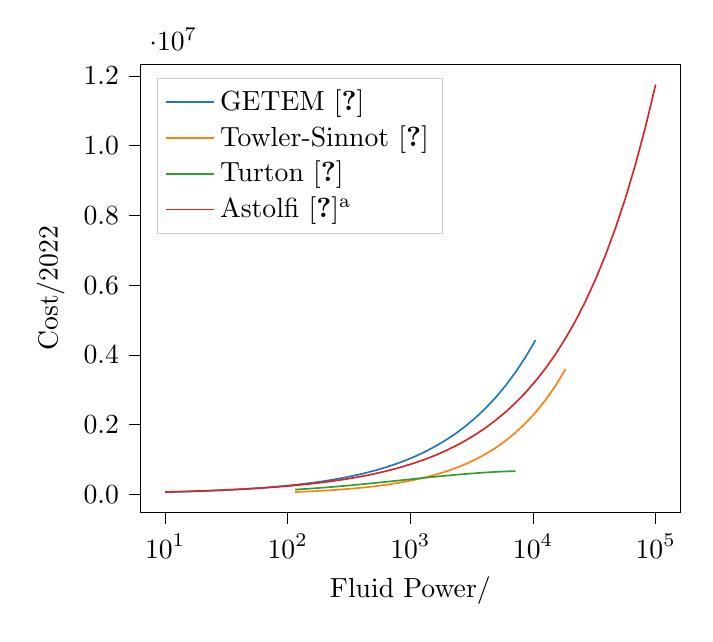
\begin{tikzpicture}

\definecolor{crimson2143940}{RGB}{214,39,40}
\definecolor{darkgray176}{RGB}{176,176,176}
\definecolor{darkorange25512714}{RGB}{255,127,14}
\definecolor{forestgreen4416044}{RGB}{44,160,44}
\definecolor{lightgray204}{RGB}{204,204,204}
\definecolor{steelblue31119180}{RGB}{31,119,180}

\begin{axis}[
legend cell align={left},
legend style={
  fill opacity=0.8,
  draw opacity=1,
  text opacity=1,
  at={(0.03,0.97)},
  anchor=north west,
  draw=lightgray204
},
log basis x={10},
tick align=outside,
tick pos=left,
unbounded coords=jump,
x grid style={darkgray176},
xlabel={Fluid Power/\unit{\kilo\watt}},
xmin=6.30957344480193, xmax=158489.319246111,
xmode=log,
xtick style={color=black},
xtick={0.1,1,10,100,1000,10000,100000,1000000,10000000},
xticklabels={
  \(\displaystyle {10^{-1}}\),
  \(\displaystyle {10^{0}}\),
  \(\displaystyle {10^{1}}\),
  \(\displaystyle {10^{2}}\),
  \(\displaystyle {10^{3}}\),
  \(\displaystyle {10^{4}}\),
  \(\displaystyle {10^{5}}\),
  \(\displaystyle {10^{6}}\),
  \(\displaystyle {10^{7}}\)
},
y grid style={darkgray176},
ylabel={Cost/\unit{\USD}2022},
ymin=-524986.649421086, ymax=12340066.2524408,
ytick style={color=black},
ytick={-2000000,0,2000000,4000000,6000000,8000000,10000000,12000000,14000000},
yticklabels={\ensuremath{-}0.2,0.0,0.2,0.4,0.6,0.8,1.0,1.2,1.4}
]
\addplot [semithick, steelblue31119180]
table {%
10 59788.4824817265
12.0679264063933 67123.0393006052
14.5634847750124 75359.6324932257
17.5751062485479 84609.4948622484
21.2095088792019 94997.6142710276
25.5954792269954 106664.439612931
30.8884359647748 119767.799013301
37.2759372031494 134485.05675104
44.9843266896944 151015.538703222
54.2867543932386 169583.259849204
65.5128556859551 190439.991572964
79.060432109077 213868.711232913
95.4095476349994 240187.481793977
115.139539932645 269753.815312304
138.949549437314 302969.580813195
167.683293681101 340286.524703028
202.358964772516 382212.480413484
244.205309454865 429318.353612282
294.705170255181 482245.980165192
355.648030622313 541716.966253057
429.193426012878 608542.633807993
517.947467923121 683635.209930004
625.055192527397 768020.416398915
754.312006335462 862851.635054618
910.298177991522 969425.8469605
1098.54114198756 1089201.56820559
1325.71136559011 1223819.03329524
1599.85871960606 1375122.90872839
1930.69772888325 1545187.85501252
2329.95181051537 1736347.29553391
2811.76869797423 1951225.79595447
3393.22177189533 2192775.50879269
4094.91506238042 2464317.19529524
4941.71336132383 2769586.40143816
5963.62331659464 3112785.43783989
7196.85673001151 3498641.89556677
8685.11373751352 3932474.52244453
10481.1313415469 4420267.38888457
12648.552168553 nan
15264.1796717523 nan
18420.6996932672 nan
22229.9648252619 nan
26826.9579527973 nan
32374.5754281764 nan
39069.3993705461 nan
47148.6636345739 nan
56898.6602901829 nan
68664.88450043 nan
82864.2772854684 nan
100000 nan
};
\addlegendentry{GETEM \cite{GETEM2016}}
\addplot [semithick, darkorange25512714]
table {%
10 nan
12.0679264063933 nan
14.5634847750124 nan
17.5751062485479 nan
21.2095088792019 nan
25.5954792269954 nan
30.8884359647748 nan
37.2759372031494 nan
44.9843266896944 nan
54.2867543932386 nan
65.5128556859551 nan
79.060432109077 nan
95.4095476349994 nan
115.139539932645 63335.4835020017
138.949549437314 75467.4169450851
167.683293681101 89436.0692963859
202.358964772516 105519.511348464
244.205309454865 124037.912532561
294.705170255181 145359.914458811
355.648030622313 169909.969381125
429.193426012878 198176.789671889
517.947467923121 230723.076508262
625.055192527397 268196.721436821
754.312006335462 311343.703803557
910.298177991522 361022.940795436
1098.54114198756 418223.385709934
1325.71136559011 484083.714823912
1599.85871960606 559914.994763872
1930.69772888325 647226.781611778
2329.95181051537 747757.171295429
2811.76869797423 863507.399469679
3393.22177189533 996781.679660497
4094.91506238042 1150233.07272075
4941.71336132383 1326916.30071056
5963.62331659464 1530348.55655617
7196.85673001151 1764579.52001141
8685.11373751352 2034271.97371357
10481.1313415469 2344794.6241393
12648.552168553 2702328.97522614
15264.1796717523 3113992.38216869
18420.6996932672 3587979.73499341
22229.9648252619 nan
26826.9579527973 nan
32374.5754281764 nan
39069.3993705461 nan
47148.6636345739 nan
56898.6602901829 nan
68664.88450043 nan
82864.2772854684 nan
100000 nan
};
\addlegendentry{Towler-Sinnot \cite{TowlerGavin2013}}
\addplot [semithick, forestgreen4416044]
table {%
10 nan
12.0679264063933 nan
14.5634847750124 nan
17.5751062485479 nan
21.2095088792019 nan
25.5954792269954 nan
30.8884359647748 nan
37.2759372031494 nan
44.9843266896944 nan
54.2867543932386 nan
65.5128556859551 nan
79.060432109077 nan
95.4095476349994 nan
115.139539932645 133245.078454807
138.949549437314 151787.240953468
167.683293681101 171969.862119461
202.358964772516 193777.079213165
244.205309454865 217162.810822553
294.705170255181 242047.994847198
355.648030622313 268318.433946475
429.193426012878 295823.395729513
517.947467923121 324375.101986061
625.055192527397 353749.220660979
754.312006335462 383686.446270814
910.298177991522 413895.219702568
1098.54114198756 444055.597926169
1325.71136559011 473824.239622109
1599.85871960606 502840.425973717
1930.69772888325 530732.989083496
2329.95181051537 557127.976002622
2811.76869797423 581656.836610475
3393.22177189533 603964.890842895
4094.91506238042 623719.807088959
4941.71336132383 640619.810612618
5963.62331659464 654401.3397526
7196.85673001151 664845.878952853
8685.11373751352 nan
10481.1313415469 nan
12648.552168553 nan
15264.1796717523 nan
18420.6996932672 nan
22229.9648252619 nan
26826.9579527973 nan
32374.5754281764 nan
39069.3993705461 nan
47148.6636345739 nan
56898.6602901829 nan
68664.88450043 nan
82864.2772854684 nan
100000 nan
};
\addlegendentry{Turton \cite{Turton2012}}
\addplot [semithick, crimson2143940]
table {%
10 64653.3163168255
12.0679264063933 71814.1758316322
14.5634847750124 79770.9519022951
17.5751062485479 88612.4781483075
21.2095088792019 98437.5515828551
25.5954792269954 109356.056440862
30.8884359647748 121490.215598201
37.2759372031494 134975.984175167
44.9843266896944 149964.601600174
54.2867543932386 166624.320288395
65.5128556859551 185142.331187596
79.060432109077 205726.908785633
95.4095476349994 228609.800789613
115.139539932645 254048.890607977
138.949549437314 282331.164029648
167.683293681101 313776.015139448
202.358964772516 348738.930581275
244.205309454865 387615.595830742
294.705170255181 430846.472223774
355.648030622313 478921.899170401
429.193426012878 532387.782334881
517.947467923121 591851.935663786
625.055192527397 657991.153082109
754.312006335462 731559.094553557
910.298177991522 813395.081127094
1098.54114198756 904433.90469284
1325.71136559011 1005716.77058728
1599.85871960606 1118403.50507804
1930.69772888325 1243786.17529902
2329.95181051537 1383304.28659539
2811.76869797423 1538561.74169731
3393.22177189533 1711345.7679206
4094.91506238042 1903648.04297058
4941.71336132383 2117688.277217
5963.62331659464 2355940.54086408
7196.85673001151 2621162.6586551
8685.11373751352 2916429.03306967
10481.1313415469 3245167.29988993
12648.552168553 3611199.26808874
15264.1796717523 4018786.64985402
18420.6996932672 4472682.14691443
22229.9648252619 4978186.52695965
26826.9579527973 5541212.39974543
32374.5754281764 6168355.48743119
39069.3993705461 6866974.27894149
47148.6636345739 7645279.06492523
56898.6602901829 8512431.4696264
68664.88450043 9478655.73026279
82864.2772854684 10555363.1251224
100000 11755291.120538
};
\addlegendentry{Astolfi \cite{Astolfi2014B}\textsuperscript{a}}
\end{axis}

\end{tikzpicture}

        %     \caption[ORC turbine cost correlations.]{ORC turbine cost correlations. \textsuperscript{a}Assuming n-Butane as the working fluid, \num{3} turbine stages, \(\Delta h=\)\qty{78.74}{\kilo\watt\per\kg}, and an outlet vapour density of \qty{10.45}{\kg\per\m\cubed}}
        %     \label{fig:prosim_litrev_ORCturb_cost}
        % \end{figure}

        \begin{figure}[H]
            \centering
            % This file was created with tikzplotlib v0.10.1.
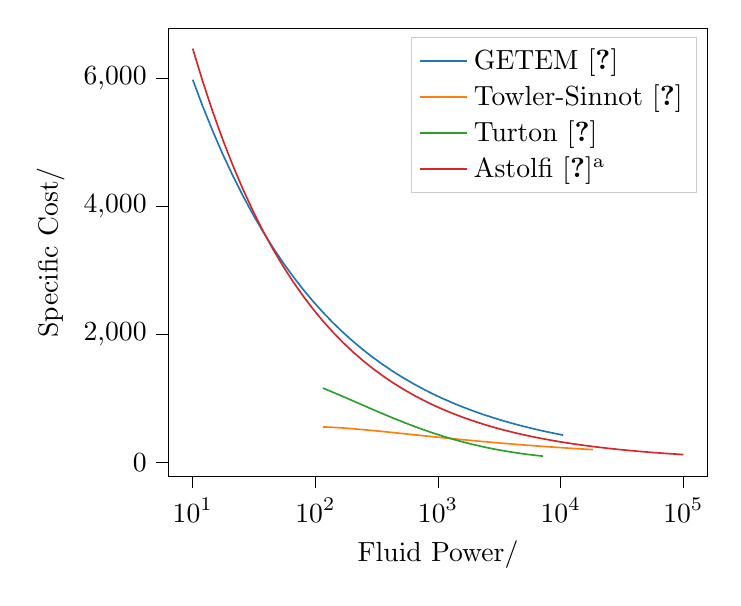
\begin{tikzpicture}

\definecolor{crimson2143940}{RGB}{214,39,40}
\definecolor{darkgray176}{RGB}{176,176,176}
\definecolor{darkorange25512714}{RGB}{255,127,14}
\definecolor{forestgreen4416044}{RGB}{44,160,44}
\definecolor{lightgray204}{RGB}{204,204,204}
\definecolor{steelblue31119180}{RGB}{31,119,180}

\begin{axis}[
legend cell align={left},
legend style={fill opacity=0.8, draw opacity=1, text opacity=1, draw=lightgray204},
log basis x={10},
tick align=outside,
tick pos=left,
unbounded coords=jump,
x grid style={darkgray176},
xlabel={Fluid Power/\unit{\kilo\watt}},
xmin=6.30957344480193, xmax=158489.319246111,
xmode=log,
xtick style={color=black},
xtick={0.1,1,10,100,1000,10000,100000,1000000,10000000},
xticklabels={
  \(\displaystyle {10^{-1}}\),
  \(\displaystyle {10^{0}}\),
  \(\displaystyle {10^{1}}\),
  \(\displaystyle {10^{2}}\),
  \(\displaystyle {10^{3}}\),
  \(\displaystyle {10^{4}}\),
  \(\displaystyle {10^{5}}\),
  \(\displaystyle {10^{6}}\),
  \(\displaystyle {10^{7}}\)
},
y grid style={darkgray176},
ylabel={Specific Cost/\unit{\USD\per\kilo\watt}},
ymin=-226.267544492086, ymax=6783.97921150039,
ytick style={color=black}
]
\addplot [semithick, steelblue31119180]
table {%
10 5978.84824817265
12.0679264063933 5562.10214084875
14.5634847750124 5174.56046114219
17.5751062485479 4814.16690549105
21.2095088792019 4479.01056135168
25.5954792269954 4167.31558987309
30.8884359647748 3877.43164302277
37.2759372031494 3607.82496273971
44.9843266896944 3357.07011344062
54.2867543932386 3123.84230268749
65.5128556859551 2906.91024805673
79.060432109077 2705.12955125069
95.4095476349994 2517.43654327807
115.139539932645 2342.84256711558
138.949549437314 2180.42866666422
167.683293681101 2029.34065304194
202.358964772516 1888.78452132404
244.205309454865 1758.0221927633
294.705170255181 1636.36755930553
355.648030622313 1523.18280887191
429.193426012878 1417.87501141673
517.947467923121 1319.89294719648
625.055192527397 1228.72416001128
754.312006335462 1143.89221940992
910.298177991522 1064.95417699224
1098.54114198756 991.498203003055
1325.71136559011 923.141390396456
1599.85871960606 859.527714464061
1930.69772888325 800.326136969294
2329.95181051537 745.228844518394
2811.76869797423 693.949611630663
3393.22177189533 646.222279650142
4094.91506238042 601.799343272019
4941.71336132383 560.450637043063
5963.62331659464 521.96211473956
7196.85673001151 486.134715031512
8685.11373751352 452.78330731111
10481.1313415469 421.735711999217
12648.552168553 nan
15264.1796717523 nan
18420.6996932672 nan
22229.9648252619 nan
26826.9579527973 nan
32374.5754281764 nan
39069.3993705461 nan
47148.6636345739 nan
56898.6602901829 nan
68664.88450043 nan
82864.2772854684 nan
100000 nan
};
\addlegendentry{GETEM \cite{GETEM2016}}
\addplot [semithick, darkorange25512714]
table {%
10 nan
12.0679264063933 nan
14.5634847750124 nan
17.5751062485479 nan
21.2095088792019 nan
25.5954792269954 nan
30.8884359647748 nan
37.2759372031494 nan
44.9843266896944 nan
54.2867543932386 nan
65.5128556859551 nan
79.060432109077 nan
95.4095476349994 nan
115.139539932645 550.075877835297
138.949549437314 543.128187537821
167.683293681101 533.363028200502
202.358964772516 521.447179111068
244.205309454865 507.924716335809
294.705170255181 493.23842650248
355.648030622313 477.747533379608
429.193426012878 461.742369898142
517.947467923121 445.456519815458
625.055192527397 429.076863360456
754.312006335462 412.751886737296
910.298177991522 396.598553665125
1098.54114198756 380.707986005198
1325.71136559011 365.150158163148
1599.85871960606 349.977774851109
1930.69772888325 335.229472707852
2329.95181051537 320.932462173984
2811.76869797423 307.104706049186
3393.22177189533 293.756714611592
4094.91506238042 280.893023468991
4941.71336132383 268.513408951565
5963.62331659464 256.613886443457
7196.85673001151 245.187529251897
8685.11373751352 234.225139151254
10481.1313415469 223.715794386109
12648.552168553 213.647296482258
15264.1796717523 204.006533540181
18420.6996932672 194.779774641504
22229.9648252619 nan
26826.9579527973 nan
32374.5754281764 nan
39069.3993705461 nan
47148.6636345739 nan
56898.6602901829 nan
68664.88450043 nan
82864.2772854684 nan
100000 nan
};
\addlegendentry{Towler-Sinnot \cite{TowlerGavin2013}}
\addplot [semithick, forestgreen4416044]
table {%
10 nan
12.0679264063933 nan
14.5634847750124 nan
17.5751062485479 nan
21.2095088792019 nan
25.5954792269954 nan
30.8884359647748 nan
37.2759372031494 nan
44.9843266896944 nan
54.2867543932386 nan
65.5128556859551 nan
79.060432109077 nan
95.4095476349994 nan
115.139539932645 1157.24866134391
138.949549437314 1092.39102658585
167.683293681101 1025.56347948718
202.358964772516 957.590781466007
244.205309454865 889.263265026144
294.705170255181 821.322525959121
355.648030622313 754.449373660166
429.193426012878 689.254256472785
517.947467923121 626.270272710761
625.055192527397 565.948775228316
754.312006335462 508.657482644096
910.298177991522 454.68092731525
1098.54114198756 404.223001719127
1325.71136559011 357.411312839728
1599.85871960606 314.30301926756
1930.69772888325 274.891807839066
2329.95181051537 239.115664748186
2811.76869797423 206.86510843852
3393.22177189533 177.991575984007
4094.91506238042 152.315688503288
4941.71336132383 129.635161688335
5963.62331659464 109.732172039041
7196.85673001151 92.3800353257539
8685.11373751352 nan
10481.1313415469 nan
12648.552168553 nan
15264.1796717523 nan
18420.6996932672 nan
22229.9648252619 nan
26826.9579527973 nan
32374.5754281764 nan
39069.3993705461 nan
47148.6636345739 nan
56898.6602901829 nan
68664.88450043 nan
82864.2772854684 nan
100000 nan
};
\addlegendentry{Turton \cite{Turton2012}}
\addplot [semithick, crimson2143940]
table {%
10 6465.33163168255
12.0679264063933 5950.82977913975
14.5634847750124 5477.46319886045
17.5751062485479 5041.93129163181
21.2095088792019 4641.19900859106
25.5954792269954 4272.47544267602
30.8884359647748 3933.19414866939
37.2759372031494 3620.99505210463
44.9843266896944 3333.7078186063
54.2867543932386 3069.33656562729
65.5128556859551 2826.04580809454
79.060432109077 2602.14753825021
95.4095476349994 2396.0893480408
115.139539932645 2206.44350981941
138.949549437314 2031.89693793876
167.683293681101 1871.24196007377
202.358964772516 1723.36783286727
244.205309454865 1587.25294178087
294.705170255181 1461.95762989401
355.648030622313 1346.61760486171
429.193426012878 1240.43787734742
517.947467923121 1142.68718802123
625.055192527397 1052.69288368206
754.312006335462 969.83620625046
910.298177991522 893.54796130842
1098.54114198756 823.30453555565
1325.71136559011 758.62423502691
1599.85871960606 699.063918189869
1930.69772888325 644.215900133912
2329.95181051537 593.705105982173
2811.76869797423 547.186453425484
3393.22177189533 504.342445900526
4094.91506238042 464.880959426779
4941.71336132383 428.533207488525
5963.62331659464 395.051869608923
7196.85673001151 364.209370422038
8685.11373751352 335.796297113849
10481.1313415469 309.619944082391
12648.552168553 285.502974567078
15264.1796717523 263.28218982453
18420.6996932672 242.807397188567
22229.9648252619 223.940369050989
26826.9579527973 206.553885442223
32374.5754281764 190.530853481486
39069.3993705461 175.763497508959
47148.6636345739 162.152614211508
56898.6602901829 149.606887512167
68664.88450043 138.042258415267
82864.2772854684 127.381345386735
100000 117.55291120538
};
\addlegendentry{Astolfi \cite{Astolfi2014B}\textsuperscript{a}}
\end{axis}

\end{tikzpicture}

            \caption[ORC turbine specific cost correlations.]{ORC turbine specific cost correlations. \textsuperscript{a}Assuming n-Butane as the working fluid, \num{3} turbine stages, \(\Delta h=\)\qty{78.74}{\kilo\watt}, and an outlet vapour density of \qty{10.45}{\kg\per\m\cubed}}
            \label{fig:prosim_litrev_ORCturb_speccost}
        \end{figure}

        From Figure~\ref{fig:prosim_litrev_ORCturb_speccost} it can be seen that the generic model from \emph{GETEM} and the \emph{Similitude} approach yield comparable costs estimates over a wide range of turbine capacities. However, for other fluids or expansion processes agreement between the two approaches may differ.
    
    \subsection{Shell \& Tube Heat Exchangers}

        Shell and Tube heat exchangers are common process equipment that have been in use for many decades, resulting in extensive design, manufacturing and operational experience. As a result, cost correlations have been published in a number of reference text books, see Table~\ref{table:ShellAndTubeCosts}, the main challenge being to accurately update the purchasing costs to today's cost levels.
        
        \begin{table}[H]
            \caption[Cost correlations for shell and tube heat exchangers.]{Cost correlations for shell and tube heat exchangers.\(A\) is the heat transfer area in \unit{\square\m}. \textsuperscript{a}Floating head \textsuperscript{b}Fixed head \textsuperscript{c}Fixed or floating head \textsuperscript{d}Kettle boiler \textsuperscript{e}Primary heat exchanger \textsuperscript{f}Recuperator}
            \centering 
            \label{table:ShellAndTubeCosts}
            \scalebox{0.8}{
                % \begin{tabular}{|c | c c | c | c | c |}
%     \hline
%     \rowcolor{bluepoli!40} % comment this line to remove the color
%     \textbf{Cost Correlation} & \textbf{Min}/\unit{\square\m} & \textbf{Max}/\unit{\square\m} & \textbf{Currency} & \textbf{Reference} \T\B \\
%     \hline \hline
%     \(C = 3.28\cdot10^4 *\left(\frac{A}{80}\right)^{0.68}\) & 80 & 4000 & \$2000 & \cite{Smith2005} \T\B \\ % Heat transfer Area
%     \(C = 181 * A + 3320\) & - & - & \$2002 & \cite{Peters2003, Adams2021} \textsuperscript{a} \T\B \\ % fixed head
%     \(C = 239 * A + 13400\) & - & - & \$2002 & \cite{Peters2003, Adams2021} \textsuperscript{b} \T\B \\ % floating head
%     \(C = 235 * A + 17900\) & - & - & \$2002 &\cite{Loh2002, Adams2021} \textsuperscript{c} \T\B \\ % flaoting/fixed head

%     \hline
% \end{tabular}

\begin{tabular}{|c | c c | c | c | c |}
    \hline
    \rowcolor{bluepoli!40} % comment this line to remove the color
    \textbf{Cost Correlation} & \textbf{Min}/\unit{\square\m} & \textbf{Max}/\unit{\square\m} & \textbf{Currency} & \textbf{Reference} \T\B \\
    \hline \hline
    \(C = 3.28\cdot10^4 *\left(\frac{A}{80}\right)^{0.68}\) & 80 & 4000 & \$2000 & \cite{Smith2005} \T\B \\ % Heat transfer Area
    \(C = 239 * A + 13400\) & - & - & \$2002 & \cite{Peters2003, Adams2021} \textsuperscript{a} \T\B \\ % floating head
    \(C = 181 * A + 3320\) & - & - & \$2002 & \cite{Peters2003, Adams2021} \textsuperscript{b} \T\B \\ % fixed head
    \(C = 235 * A + 17900\) & - & - & \$2002 &\cite{Loh2002, Adams2021} \textsuperscript{c} \T\B \\ % flaoting/fixed head
    \(\log C = 4.3247 - 0.3030\log A + 0.1634(\log A)^2\) & 10 & 1000 & \$2001 & \cite{Turton2012}\textsuperscript{a} \T\B \\ % heat exchanger
    \(\log C = 4.8306 -0.8509\log A + 0.3187(\log A)^2\) & 10 & 1000 & \$2001 & \cite{Turton2012}\textsuperscript{b} \T\B \\ % heat exchanger
    \(\log C = 4.4646 -0.5277\log A + 0.3955(\log A)^2\) & 10 & 100 & \$2001 & \cite{Turton2012} \textsuperscript{d} \T\B \\ % kettle boiler
    \(C = 1500 * \left(\frac{UA}{4000}\right)^{0.9}*10^{f_P}\) & - & - & \euro2014 & \cite{Astolfi2014B} \textsuperscript{e} \T\B \\ % PHE
    \(f_P= 0.03881 - 0.11272*\log P + 0.08183* \log^2 P\) &  &  &  &  \T\B \\ 
    \(C = 260 *\left(\frac{UA}{650}\right)^{0.9}*10^{f_P}\) & - & - & \euro2014 & \cite{Astolfi2014B} \textsuperscript{f} \T\B \\ % RECU
    \(f_P= -0.00164 - 0.00627*\log P +0.0123* \log^2 P\) &  &  &  &  \T\B \\ 

    \hline
\end{tabular}
            }
            \\[10pt]
        \end{table}

        As can be seen from Figure~\ref{fig:prosim_litrev_SandTHX_speccost} the different correlations yield remarkably similar results over a wide range of heat transfer areas. Owing to most the majority of the cost models scaling linearly to the heat transfer area, the specific cost for heat exchangers larger than \qty{10}{\square\m} remains fairly constant at around \qty{225}{\USD\per\square\m}.

        % \begin{figure}[H]
        %     \centering
        %     % This file was created with tikzplotlib v0.10.1.
\begin{tikzpicture}

\definecolor{crimson2143940}{RGB}{214,39,40}
\definecolor{darkgray176}{RGB}{176,176,176}
\definecolor{darkorange25512714}{RGB}{255,127,14}
\definecolor{forestgreen4416044}{RGB}{44,160,44}
\definecolor{goldenrod18818934}{RGB}{188,189,34}
\definecolor{gray127}{RGB}{127,127,127}
\definecolor{lightgray204}{RGB}{204,204,204}
\definecolor{mediumpurple148103189}{RGB}{148,103,189}
\definecolor{orchid227119194}{RGB}{227,119,194}
\definecolor{sienna1408675}{RGB}{140,86,75}
\definecolor{steelblue31119180}{RGB}{31,119,180}

\begin{axis}[
legend cell align={left},
legend style={
  fill opacity=0.8,
  draw opacity=1,
  text opacity=1,
  at={(1.03,0.5)},
  anchor=west,
  draw=lightgray204
},
log basis x={10},
tick align=outside,
tick pos=left,
unbounded coords=jump,
x grid style={darkgray176},
xlabel={Heat Transfer Area/\unit{\square\m}},
xmin=7.07945784384138, xmax=14125.3754462276,
xmode=log,
xtick style={color=black},
xtick={0.1,1,10,100,1000,10000,100000,1000000},
xticklabels={
  \(\displaystyle {10^{-1}}\),
  \(\displaystyle {10^{0}}\),
  \(\displaystyle {10^{1}}\),
  \(\displaystyle {10^{2}}\),
  \(\displaystyle {10^{3}}\),
  \(\displaystyle {10^{4}}\),
  \(\displaystyle {10^{5}}\),
  \(\displaystyle {10^{6}}\)
},
y grid style={darkgray176},
ylabel={Cost/\unit{\USD}2023},
ymin=-283325.074453396, ymax=6088024.18060106,
ytick style={color=black},
ytick={-1000000,0,1000000,2000000,3000000,4000000,5000000,6000000,7000000},
yticklabels={\ensuremath{-}1,0,1,2,3,4,5,6,7},
width=10cm, height=6.5cm
]
\addplot [semithick, steelblue31119180]
table {%
10 nan
11.5139539932645 nan
13.2571136559011 nan
15.2641796717523 nan
17.5751062485479 nan
20.2358964772516 nan
23.2995181051537 nan
26.8269579527973 nan
30.8884359647748 nan
35.5648030622313 nan
40.9491506238043 nan
47.1486636345739 nan
54.2867543932386 nan
62.5055192527397 nan
71.9685673001152 nan
82.8642772854684 81048.665100301
95.4095476349994 89202.806695768
109.854114198756 98177.3199170556
126.48552168553 108054.74068736
145.634847750124 118925.908701488
167.683293681101 130890.802851458
193.069772888325 144059.460702569
222.29964825262 158552.99047609
255.954792269954 174504.684845477
294.705170255181 192061.246789358
339.322177189533 211384.138775108
390.693993705462 232651.067681031
449.843266896944 256057.619113556
517.947467923121 281819.056149764
596.362331659464 310172.299047746
686.6488450043 341378.104131603
790.60432109077 375723.46188964
910.298177991522 413524.236340344
1048.11313415469 455128.069939622
1206.79264063933 500917.580744846
1389.49549437314 551313.881239092
1599.85871960606 606780.451177123
1842.06996932672 667827.400070563
2120.95088792019 735016.158513022
2442.05309454865 808964.641489938
2811.76869797423 890352.931158519
3237.45754281764 979929.531360644
3727.59372031494 1078518.2513896
4291.93426012878 nan
4941.71336132383 nan
5689.86602901829 nan
6551.28556859551 nan
7543.12006335462 nan
8685.11373751352 nan
10000 nan
};
\addlegendentry{Smith \cite{Smith2005}}
\addplot [semithick, darkorange25512714]
table {%
10 48854.9356223176
11.5139539932645 49713.2847258179
13.2571136559011 50701.5839346041
15.2641796717523 51839.5070967584
17.5751062485479 53149.70659045
20.2358964772516 54658.2642596863
23.2995181051537 56395.2106196636
26.8269579527973 58395.1226674183
30.8884359647748 60697.8121982606
35.5648030622313 63349.1183301495
40.9491506238043 66401.8200126125
47.1486636345739 69916.6866853165
54.2867543932386 73963.6880015136
62.5055192527397 78623.3866980512
71.9685673001152 83988.5423394919
82.8642772854684 90165.9578617171
95.4095476349994 97278.6056737351
109.854114198756 105468.075641522
126.48552168553 114897.393685354
145.634847750124 125754.267099807
167.683293681101 138254.821200279
193.069772888325 152647.901680593
222.29964825262 169220.028327763
255.954792269954 188301.098706369
294.705170255181 210270.95535452
339.322177189533 235566.947223062
390.693993705462 264692.635881902
449.843266896944 298227.819805904
517.947467923121 336840.076291566
596.362331659464 381298.05076677
686.6488450043 432486.758040893
790.60432109077 491425.200093786
910.298177991522 559286.651116956
1048.11313415469 637422.01361665
1206.79264063933 727386.710523503
1389.49549437314 830971.648643851
1599.85871960606 950238.869835134
1842.06996932672 1087562.59960523
2120.95088792019 1245676.51028086
2442.05309454865 1427728.1396023
2811.76869797423 1637341.54804289
3237.45754281764 1878689.46215852
3727.59372031494 2156576.34010829
4291.93426012878 2476534.01291284
4941.71336132383 2844931.8053592
5689.86602901829 3269103.32870396
6551.28556859551 3757492.4692084
7543.12006335462 4319821.47866622
8685.11373751352 4967284.51306375
10000 5712770.47210301
};
\addlegendentry{NETL \cite{Loh2002, Adams2021}\textsuperscript{a}}
\addplot [semithick, forestgreen4416044]
table {%
10 38094.7868383405
11.5139539932645 38967.7461393471
13.2571136559011 39972.8674623254
15.2641796717523 41130.1595293675
17.5751062485479 42462.6602910368
20.2358964772516 43996.8955376218
23.2995181051537 45763.4069420243
26.8269579527973 47797.360045911
30.8884359647748 50139.2442921718
35.5648030622313 52835.6790390717
40.9491506238043 55940.3416012361
47.1486636345739 59515.0357917734
54.2867543932386 63630.9222367569
62.5055192527397 68369.934953661
71.9685673001152 73826.412393254
82.8642772854684 80108.9754137298
95.4095476349994 87342.6895714842
109.854114198756 95671.5547727652
126.48552168553 105261.37184713
145.634847750124 116303.043106936
167.683293681101 129016.372596352
193.069772888325 143654.441680587
222.29964825262 160508.647079197
255.954792269954 179914.50163446
294.705170255181 202258.313289389
339.322177189533 227984.87523229
390.693993705462 257606.320293832
449.843266896944 291712.315859094
517.947467923121 330981.802242385
596.362331659464 376196.508198018
686.6488450043 428256.512617232
790.60432109077 488198.16219443
910.298177991522 557214.701745653
1048.11313415469 636680.027862364
1206.79264063933 728176.038759121
1389.49549437314 833524.124762368
1599.85871960606 954821.426314354
1842.06996932672 1094482.58127202
2120.95088792019 1255287.7925549
2442.05309454865 1440438.17301373
2811.76869797423 1653619.46925756
3237.45754281764 1899075.43297516
3727.59372031494 2181692.30033683
4291.93426012878 2507096.06118913
4941.71336132383 2881764.45435798
5689.86602901829 3313155.91852563
6551.28556859551 3809858.06567696
7543.12006335462 4381758.63274256
8685.11373751352 5040242.31453409
10000 5798417.3962804
};
\addlegendentry{Peters \cite{Peters2003, Adams2021}\textsuperscript{b}}
\addplot [semithick, crimson2143940]
table {%
10 12376.5836909871
11.5139539932645 13037.6951281512
13.2571136559011 13798.8957953439
15.2641796717523 14675.3387415139
17.5751062485479 15684.4711175061
20.2358964772516 16846.3814925349
23.2995181051537 18184.1997527728
26.8269579527973 19724.5575427455
30.8884359647748 21498.1184154368
35.5648030622313 23540.1882446789
40.9491506238043 25891.4180511717
47.1486636345739 28598.6132331267
54.2867543932386 31715.6653107083
62.5055192527397 35304.6247322968
71.9685673001152 39436.9360986831
82.8642772854684 44194.8603945246
95.4095476349994 49673.1125391001
109.854114198756 55980.7468547146
126.48552168553 63243.3279863467
145.634847750124 71605.430488543
167.683293681101 81233.516838268
193.069772888325 92319.2511656591
222.29964825262 105083.314668373
255.954792269954 119779.798662107
294.705170255181 136701.262718768
339.322177189533 156184.558583476
390.693993705462 178617.535805816
449.843266896944 204446.762572813
517.947467923121 234186.415440493
596.362331659464 268428.514929906
686.6488450043 307854.710745294
790.60432109077 353249.851220076
910.298177991522 405517.607114517
1048.11313415469 465698.460784494
1206.79264063933 534990.418827645
1389.49549437314 614772.860528849
1599.85871960606 706633.996850646
1842.06996932672 812402.486588464
2120.95088792019 934183.839066292
2442.05309454865 1074402.32803302
2811.76869797423 1235849.25112981
3237.45754281764 1421738.49561887
3727.59372031494 1635770.51650784
4291.93426012878 1882206.00066794
4941.71336132383 2165950.68336067
5689.86602901829 2492653.00559642
6551.28556859551 2868816.55636793
7543.12006335462 3301929.53812055
8685.11373751352 3800613.83269907
10000 4374796.63519313
};
\addlegendentry{Peters \cite{Peters2003, Adams2021}\textsuperscript{c}}
\addplot [semithick, mediumpurple148103189]
table {%
10 36947.3604759323
11.5139539932645 37123.8539504014
13.2571136559011 37406.5523720989
15.2641796717523 37797.8676069801
17.5751062485479 38301.1581109986
20.2358964772516 38920.7770126433
23.2995181051537 39662.13491567
26.8269579527973 40531.7786915178
30.8884359647748 41537.4878688169
35.5648030622313 42688.3906074866
40.9491506238043 43995.1016777298
47.1486636345739 45469.885361979
54.2867543932386 47126.8467749011
62.5055192527397 48982.1557699135
71.9685673001152 51054.308390545
82.8642772854684 53364.43175559
95.4095476349994 55936.6393674391
109.854114198756 58798.4451382589
126.48552168553 61981.2459811849
145.634847750124 65520.8846646748
167.683293681101 69458.3068399317
193.069772888325 73840.328799578
222.29964825262 78720.5357028886
255.954792269954 84160.333821597
294.705170255181 90230.1849584617
339.322177189533 97011.0567373504
390.693993705462 104596.129165964
449.843266896944 113092.805985344
517.947467923121 122625.089158015
596.362331659464 133336.386796181
686.6488450043 145392.83937149
790.60432109077 158987.266770692
910.298177991522 174343.860401553
1048.11313415469 nan
1206.79264063933 nan
1389.49549437314 nan
1599.85871960606 nan
1842.06996932672 nan
2120.95088792019 nan
2442.05309454865 nan
2811.76869797423 nan
3237.45754281764 nan
3727.59372031494 nan
4291.93426012878 nan
4941.71336132383 nan
5689.86602901829 nan
6551.28556859551 nan
7543.12006335462 nan
8685.11373751352 nan
10000 nan
};
\addlegendentry{Turton \cite{Turton2012}\textsuperscript{a}}
\addplot [semithick, sienna1408675]
table {%
10 47960.468604936
11.5139539932645 46666.6489899994
13.2571136559011 45658.2298004642
15.2641796717523 44918.0378973173
17.5751062485479 44433.6243722527
20.2358964772516 44196.9149783664
23.2995181051537 44203.9854155278
26.8269579527973 44454.9526987188
30.8884359647748 44953.9783916106
35.5648030622313 45709.3838307106
40.9491506238043 46733.881814719
47.1486636345739 48044.9338068759
54.2867543932386 49665.2467263349
62.5055192527397 51623.429147277
71.9685673001152 53954.8334852949
82.8642772854684 56702.6188972692
95.4095476349994 59919.0796096943
109.854114198756 63667.2957968541
126.48552168553 68023.1796898253
145.634847750124 73078.0092578576
167.683293681101 78941.5667952296
193.069772888325 85746.0316737337
222.29964825262 93650.8174861541
255.954792269954 102848.596575743
294.705170255181 113572.823173524
339.322177189533 126107.154889242
390.693993705462 140797.287557736
449.843266896944 158065.869014019
517.947467923121 178431.354744956
596.362331659464 202531.927968172
686.6488450043 231155.949300266
790.60432109077 265280.854885436
910.298177991522 306123.024757088
1048.11313415469 nan
1206.79264063933 nan
1389.49549437314 nan
1599.85871960606 nan
1842.06996932672 nan
2120.95088792019 nan
2442.05309454865 nan
2811.76869797423 nan
3237.45754281764 nan
3727.59372031494 nan
4291.93426012878 nan
4941.71336132383 nan
5689.86602901829 nan
6551.28556859551 nan
7543.12006335462 nan
8685.11373751352 nan
10000 nan
};
\addlegendentry{Turton \cite{Turton2012}\textsuperscript{b}}
\addplot [semithick, orchid227119194]
table {%
10 51866.0790695367
11.5139539932645 54011.5117678878
13.2571136559011 56631.0042674539
15.2641796717523 59784.308165023
17.5751062485479 63545.5535258875
20.2358964772516 68006.1424499846
23.2995181051537 73278.4254803955
26.8269579527973 79500.366737196
30.8884359647748 86841.4666498077
35.5648030622313 95510.2939388424
40.9491506238043 105764.087863507
47.1486636345739 117921.036940429
54.2867543932386 132376.033960443
62.5055192527397 149620.966458045
71.9685673001152 170270.950599716
82.8642772854684 195098.387607057
95.4095476349994 225077.360905348
109.854114198756 nan
126.48552168553 nan
145.634847750124 nan
167.683293681101 nan
193.069772888325 nan
222.29964825262 nan
255.954792269954 nan
294.705170255181 nan
339.322177189533 nan
390.693993705462 nan
449.843266896944 nan
517.947467923121 nan
596.362331659464 nan
686.6488450043 nan
790.60432109077 nan
910.298177991522 nan
1048.11313415469 nan
1206.79264063933 nan
1389.49549437314 nan
1599.85871960606 nan
1842.06996932672 nan
2120.95088792019 nan
2442.05309454865 nan
2811.76869797423 nan
3237.45754281764 nan
3727.59372031494 nan
4291.93426012878 nan
4941.71336132383 nan
5689.86602901829 nan
6551.28556859551 nan
7543.12006335462 nan
8685.11373751352 nan
10000 nan
};
\addlegendentry{Turton \cite{Turton2012}\textsuperscript{d}}
\addplot [semithick, gray127]
table {%
10 7062.58704859496
11.5139539932645 8017.99635516461
13.2571136559011 9102.65106951462
15.2641796717523 10334.03519072
17.5751062485479 11731.9979100038
20.2358964772516 13319.0735680805
23.2995181051537 15120.8448955379
26.8269579527973 17166.3553914782
30.8884359647748 19488.5774877231
35.5648030622313 22124.9440451136
40.9491506238043 25117.9517493145
47.1486636345739 28515.8461325118
54.2867543932386 32373.3992631497
62.5055192527397 36752.7926396124
71.9685673001152 41724.6195195793
82.8642772854684 47369.0228420154
95.4095476349994 53776.987084435
109.854114198756 61051.8048794195
126.48552168553 69310.7420313908
145.634847750124 78686.9277727352
167.683293681101 89331.5007290998
193.069772888325 101416.045185567
222.29964825262 115135.35692489
255.954792269954 130710.583221484
294.705170255181 148392.787606037
339.322177189533 168466.996862662
390.693993705462 191256.795493809
449.843266896944 217129.541713032
517.947467923121 246502.289044353
596.362331659464 279848.508980934
686.6488450043 317705.7230684
790.60432109077 360684.167437505
910.298177991522 409476.629453342
1048.11313415469 464869.615042147
1206.79264063933 527756.026706422
1389.49549437314 599149.556590609
1599.85871960606 680201.026605075
1842.06996932672 772216.939001654
2120.95088792019 876680.536425162
2442.05309454865 995275.710916599
2811.76869797423 1129914.14726715
3237.45754281764 1282766.13825797
3727.59372031494 1456295.56850944
4291.93426012878 1653299.63085892
4941.71336132383 1876953.91547196
5689.86602901829 2130863.59849682
6551.28556859551 2419121.55539371
7543.12006335462 2746374.33569129
8685.11373751352 3117897.06264522
10000 3539678.46513711
};
\addlegendentry{Astolfi \cite{Astolfi2014B}\textsuperscript{e}}
\addplot [semithick, goldenrod18818934]
table {%
10 6281.70986726107
11.5139539932645 7131.48404024569
13.2571136559011 8096.21356142861
15.2641796717523 9191.44930597114
17.5751062485479 10434.8458329612
20.2358964772516 11846.4459665715
23.2995181051537 13449.0038746526
26.8269579527973 15268.3518525994
30.8884359647748 17333.8167248313
35.5648030622313 19678.6925760354
40.9491506238043 22340.7774323215
47.1486636345739 25362.9825432784
54.2867543932386 28794.0240861975
62.5055192527397 32689.2084423346
71.9685673001152 37111.3237034011
82.8642772854684 42131.6517788479
95.4095476349994 47831.1174185204
109.854114198756 54301.592672255
126.48552168553 61647.3778135437
145.634847750124 69986.8825988891
167.683293681101 79454.5349637656
193.069772888325 90202.9479222505
222.29964825262 102405.379599476
255.954792269954 116258.526051186
294.705170255181 131985.691889017
339.322177189533 149840.389820123
390.693993705462 170110.427123614
449.843266896944 193122.544935425
517.947467923121 219247.685124165
596.362331659464 248906.969656899
686.6488450043 282578.488838749
790.60432109077 320805.007848755
910.298177991522 364202.715796839
1048.11313415469 413471.158331571
1206.79264063933 469404.513906524
1389.49549437314 532904.395472065
1599.85871960606 604994.383948337
1842.06996932672 686836.527750531
2120.95088792019 779750.074329103
2442.05309454865 885232.735666439
2811.76869797423 1004984.8305173
3237.45754281764 1140936.69255185
3727.59372031494 1295279.78620444
4291.93426012878 1470502.0317975
4941.71336132383 1669427.90936079
5689.86602901829 1895263.98759614
6551.28556859551 2151650.61188786
7543.12006335462 2442720.58453944
8685.11373751352 2773165.78312747
10000 3148312.79082172
};
\addlegendentry{Astolfi \cite{Astolfi2014B}\textsuperscript{f, g}}
\end{axis}

\end{tikzpicture}

        %     \caption[Shell and tube cost correlations.]{Shell and tube cost correlations. \textsuperscript{a}Floating head \textsuperscript{b}Fixed head \textsuperscript{c}Fixed/floating head \textsuperscript{d}Kettle boiler \textsuperscript{e}Assuming an overall heat transfer coefficient of \qty{1000}{\watt\per\square\m\per\K} \textsuperscript{f}\ac{PHE} \textsuperscript{g}Recuperator.}
        %     \label{fig:prosim_litrev_SandTHX_cost}
        % \end{figure}

        \begin{figure}[H]
            \centering
            % This file was created with tikzplotlib v0.10.1.
\begin{tikzpicture}

\definecolor{crimson2143940}{RGB}{214,39,40}
\definecolor{darkgray176}{RGB}{176,176,176}
\definecolor{darkorange25512714}{RGB}{255,127,14}
\definecolor{forestgreen4416044}{RGB}{44,160,44}
\definecolor{goldenrod18818934}{RGB}{188,189,34}
\definecolor{gray127}{RGB}{127,127,127}
\definecolor{lightgray204}{RGB}{204,204,204}
\definecolor{mediumpurple148103189}{RGB}{148,103,189}
\definecolor{orchid227119194}{RGB}{227,119,194}
\definecolor{sienna1408675}{RGB}{140,86,75}
\definecolor{steelblue31119180}{RGB}{31,119,180}

\begin{axis}[
legend cell align={left},
legend style={fill opacity=0.8, draw opacity=1, text opacity=1, draw=lightgray204},
log basis x={10},
tick align=outside,
tick pos=left,
unbounded coords=jump,
x grid style={darkgray176},
xlabel={Heat Transfer Area/\unit{\square\m}},
xmin=7.07945784384138, xmax=14125.3754462276,
xmode=log,
xtick style={color=black},
xtick={0.1,1,10,100,1000,10000,100000,1000000},
xticklabels={
  \(\displaystyle {10^{-1}}\),
  \(\displaystyle {10^{0}}\),
  \(\displaystyle {10^{1}}\),
  \(\displaystyle {10^{2}}\),
  \(\displaystyle {10^{3}}\),
  \(\displaystyle {10^{4}}\),
  \(\displaystyle {10^{5}}\),
  \(\displaystyle {10^{6}}\)
},
y grid style={darkgray176},
ylabel={Specific Cost/\unit{\USD\per\square\m}},
ymin=-58.2302966684393, ymax=5436.36210712615,
ytick style={color=black}
]
\addplot [semithick, steelblue31119180]
table {%
10 nan
11.5139539932645 nan
13.2571136559011 nan
15.2641796717523 nan
17.5751062485479 nan
20.2358964772516 nan
23.2995181051537 nan
26.8269579527973 nan
30.8884359647748 nan
35.5648030622313 nan
40.9491506238043 nan
47.1486636345739 nan
54.2867543932386 nan
62.5055192527397 nan
71.9685673001152 nan
82.8642772854684 978.089325766849
95.4095476349994 934.94633301296
109.854114198756 893.706354405864
126.48552168553 854.285449017691
145.634847750124 816.603378509635
167.683293681101 780.583443812749
193.069772888325 746.152329012661
222.29964825262 713.239952120446
255.954792269954 681.779322425923
294.705170255181 651.706404143013
339.322177189533 622.959986069631
390.693993705462 595.481556996813
449.843266896944 569.215186613468
517.947467923121 544.10741166437
596.362331659464 520.107127129654
686.6488450043 497.165482204322
790.60432109077 475.235780866043
910.298177991522 454.273386828855
1048.11313415469 434.235632689297
1206.79264063933 415.08173308007
1389.49549437314 396.772701654433
1599.85871960606 379.271271732378
1842.06996932672 362.541820447058
2120.95088792019 346.550296237072
2442.05309454865 331.264149537033
2811.76869797423 316.652266525331
3237.45754281764 302.68490579425
3727.59372031494 289.333637813533
4291.93426012878 nan
4941.71336132383 nan
5689.86602901829 nan
6551.28556859551 nan
7543.12006335462 nan
8685.11373751352 nan
10000 nan
};
\addlegendentry{Smith \cite{Smith2005}}
\addplot [semithick, darkorange25512714]
table {%
10 4885.49356223176
11.5139539932645 4317.65532109122
13.2571136559011 3824.4813502097
15.2641796717523 3396.15414726098
17.5751062485479 3024.14709981291
20.2358964772516 2701.05474798861
23.2995181051537 2420.44536565712
26.8269579527973 2176.73292552089
30.8884359647748 1965.06589933787
35.5648030622313 1781.2306796498
40.9491506238043 1621.56770045463
47.1486636345739 1482.8985870566
54.2867543932386 1362.46288488239
62.5055192527397 1257.86310773836
71.9685673001152 1167.01701159692
82.8642772854684 1088.11614383716
95.4095476349994 1019.58984278896
109.854114198756 960.073970927493
126.48552168553 908.383759297079
145.634847750124 863.490222584449
167.683293681101 824.499675341607
193.069772888325 790.635941592409
222.29964825262 761.224903673543
255.954792269954 735.681082727175
294.705170255181 713.495983706187
339.322177189533 694.227972878659
390.693993705462 677.493486325386
449.843266896944 662.95939441998
517.947467923121 650.336370292987
596.362331659464 639.373130267556
686.6488450043 629.851431612303
790.60432109077 621.581728032783
910.298177991522 614.399396416418
1048.11313415469 608.16145971755
1206.79264063933 602.743740745843
1389.49549437314 598.038390199127
1599.85871960606 593.951739731817
1842.06996932672 590.402437320412
2120.95088792019 587.319827807223
2442.05309454865 584.642546384185
2811.76869797423 582.317297017543
3237.45754281764 580.297791495806
3727.59372031494 578.543827980824
4291.93426012878 577.020490718917
4941.71336132383 575.697454980892
5689.86602901829 574.548383394537
6551.28556859551 573.550401652534
7543.12006335462 572.683643158808
8685.11373751352 571.930853548711
10000 571.277047210301
};
\addlegendentry{NETL \cite{Loh2002, Adams2021}\textsuperscript{a}}
\addplot [semithick, forestgreen4416044]
table {%
10 3809.47868383405
11.5139539932645 3384.39307314783
13.2571136559011 3015.20138544882
15.2641796717523 2694.55420558777
17.5751062485479 2416.06848291715
20.2358964772516 2174.20046535035
23.2995181051537 1964.13534114689
26.8269579527973 1781.6913915477
30.8884359647748 1623.23674624868
35.5648030622313 1485.61708458275
40.9491506238043 1366.09284317407
47.1486636345739 1262.28468007164
54.2867543932386 1172.12610972893
62.5055192527397 1093.82236594514
71.9685673001152 1025.8146738616
82.8642772854684 966.749219784461
95.4095476349994 915.450201122681
109.854114198756 870.896419952642
126.48552168553 832.200954262835
145.634847750124 798.593502198632
167.683293681101 769.405047838068
193.069772888325 744.054543243697
222.29964825262 722.037341673149
255.954792269954 702.915151690952
294.705170255181 686.30731220038
339.322177189533 671.883214709381
390.693993705462 659.35572198235
449.843266896944 648.475452064336
517.947467923121 639.025813891057
596.362331659464 630.818695659729
686.6488450043 623.690720130098
790.60432109077 617.499992310793
910.298177991522 612.123274787927
1048.11313415469 607.45353446587
1206.79264063933 603.397811883698
1389.49549437314 599.875370692301
1599.85871960606 596.816090454203
1842.06996932672 594.159070771922
2120.95088792019 591.85141895758
2442.05309454865 589.847197110166
2811.76869797423 588.106507640166
3237.45754281764 586.594699037301
3727.59372031494 585.281676070778
4291.93426012878 584.141300690357
4941.71336132383 583.150871702114
5689.86602901829 582.290672860933
6551.28556859551 581.543580383679
7543.12006335462 580.89472206994
8685.11373751352 580.331181244504
10000 579.84173962804
};
\addlegendentry{Peters \cite{Peters2003, Adams2021}\textsuperscript{b}}
\addplot [semithick, crimson2143940]
table {%
10 1237.65836909871
11.5139539932645 1132.33865063019
13.2571136559011 1040.86727725998
15.2641796717523 961.423349115305
17.5751062485479 892.425393946166
20.2358964772516 832.499885116183
23.2995181051537 780.453899119506
26.8269579527973 735.251368323288
30.8884359647748 695.992456204427
35.5648030622313 661.895644508092
40.9491506238043 632.282175741166
47.1486636345739 606.562541300861
54.2867543932386 584.224746260729
62.5055192527397 564.824117203848
71.9685673001152 547.974450210015
82.8642772854684 533.340322781949
95.4095476349994 520.630416665747
109.854114198756 509.591718644513
126.48552168553 500.004483861666
145.634847750124 491.677861409938
167.683293681101 484.446095105679
193.069772888325 478.165223818118
222.29964825262 472.710215667803
255.954792269954 467.972479045348
294.705170255181 463.857700902908
339.322177189533 460.283969285735
390.693993705462 457.180142729486
449.843266896944 454.484434063232
517.947467923121 452.14318042627
596.362331659464 450.109775013732
686.6488450043 448.343739285495
790.60432109077 446.80991716907
910.298177991522 445.477775215643
1048.11313415469 444.320794777641
1206.79264063933 443.315944108029
1389.49549437314 442.443219872548
1599.85871960606 441.685248947885
1842.06996932672 441.026942578842
2120.95088792019 440.455196009916
2442.05309454865 439.9586276119
2811.76869797423 439.527352310377
3237.45754281764 439.152784805787
3727.59372031494 438.827468667813
4291.93426012878 438.544927901917
4941.71336132383 438.299538033188
5689.86602901829 438.086414141194
6551.28556859551 437.901313616979
7543.12006335462 437.740551706411
8685.11373751352 437.600928158616
10000 437.479663519313
};
\addlegendentry{Peters \citea{Peters2003, Adams2021}\textsuperscript{c}}
\addplot [semithick, mediumpurple148103189]
table {%
10 3694.73604759323
11.5139539932645 3224.24893934077
13.2571136559011 2821.62115698904
15.2641796717523 2476.24624577293
17.5751062485479 2179.28458407829
20.2358964772516 1923.35323796485
23.2995181051537 1702.27275674414
26.8269579527973 1510.86003723697
30.8884359647748 1344.75853410598
35.5648030622313 1200.29880477028
40.9491506238043 1074.38374197083
47.1486636345739 964.393937321185
54.2867543932386 868.109491931069
62.5055192527397 783.645290135984
71.9685673001152 709.39731476999
82.8642772854684 643.998035145458
95.4095476349994 586.279264014869
109.854114198756 535.241174780915
126.48552168553 490.026408993147
145.634847750124 449.898397786589
167.683293681101 414.223178201802
193.069772888325 382.454113323522
222.29964825262 354.11902952465
255.954792269954 328.809369323446
294.705170255181 306.171028083195
339.322177189533 285.896599924159
390.693993705462 267.718805129154
449.843266896944 251.404909904437
517.947467923121 236.751981141485
596.362331659464 223.582845055208
686.6488450043 211.742640258253
790.60432109077 201.095873788474
910.298177991522 191.523903504042
1048.11313415469 nan
1206.79264063933 nan
1389.49549437314 nan
1599.85871960606 nan
1842.06996932672 nan
2120.95088792019 nan
2442.05309454865 nan
2811.76869797423 nan
3237.45754281764 nan
3727.59372031494 nan
4291.93426012878 nan
4941.71336132383 nan
5689.86602901829 nan
6551.28556859551 nan
7543.12006335462 nan
8685.11373751352 nan
10000 nan
};
\addlegendentry{Turton \cite{Turton2012}\textsuperscript{a}}
\addplot [semithick, sienna1408675]
table {%
10 4796.04686049359
11.5139539932645 4053.05154226765
13.2571136559011 3444.05509265137
15.2641796717523 2942.70893446321
17.5751062485479 2528.2136986184
20.2358964772516 2184.08485277886
23.2995181051537 1897.20599439137
26.8269579527973 1657.10002516642
30.8884359647748 1455.36596423581
35.5648030622313 1285.24214658882
40.9491506238043 1141.26620705906
47.1486636345739 1019.0094501776
54.2867543932386 914.868595137836
62.5055192527397 825.901932572366
71.9685673001152 749.699980274702
82.8642772854684 684.283031902011
95.4095476349994 628.019743253809
109.854114198756 579.562233615236
126.48552168553 537.794197971098
145.634847750124 501.789306521214
167.683293681101 470.777768388545
193.069772888325 444.119399898661
222.29964825262 421.281896855411
255.954792269954 401.823289431789
294.705170255181 385.37777628802
339.322177189533 371.644305520305
390.693993705462 360.377404890131
449.843266896944 351.379870825611
517.947467923121 344.497011367649
596.362331659464 339.612207572865
686.6488450043 336.643614828797
790.60432109077 335.541873233676
910.298177991522 336.288737205337
1048.11313415469 nan
1206.79264063933 nan
1389.49549437314 nan
1599.85871960606 nan
1842.06996932672 nan
2120.95088792019 nan
2442.05309454865 nan
2811.76869797423 nan
3237.45754281764 nan
3727.59372031494 nan
4291.93426012878 nan
4941.71336132383 nan
5689.86602901829 nan
6551.28556859551 nan
7543.12006335462 nan
8685.11373751352 nan
10000 nan
};
\addlegendentry{Turton \cite{Turton2012}\textsuperscript{b}}
\addplot [semithick, orchid227119194]
table {%
10 5186.60790695367
11.5139539932645 4690.96122839155
13.2571136559011 4271.74464497753
15.2641796717523 3916.64075309982
17.5751062485479 3615.65686302111
20.2358964772516 3360.66862797181
23.2995181051537 3145.06184847603
26.8269579527973 2963.45067812307
30.8884359647748 2811.45561234767
35.5648030622313 2685.52854831555
40.9491506238043 2582.81518059193
47.1486636345739 2501.04728003272
54.2867543932386 2438.45916817105
62.5055192527397 2393.72407823788
71.9685673001152 2365.90718680937
82.8642772854684 2354.43298364795
95.4095476349994 2359.0653816577
109.854114198756 nan
126.48552168553 nan
145.634847750124 nan
167.683293681101 nan
193.069772888325 nan
222.29964825262 nan
255.954792269954 nan
294.705170255181 nan
339.322177189533 nan
390.693993705462 nan
449.843266896944 nan
517.947467923121 nan
596.362331659464 nan
686.6488450043 nan
790.60432109077 nan
910.298177991522 nan
1048.11313415469 nan
1206.79264063933 nan
1389.49549437314 nan
1599.85871960606 nan
1842.06996932672 nan
2120.95088792019 nan
2442.05309454865 nan
2811.76869797423 nan
3237.45754281764 nan
3727.59372031494 nan
4291.93426012878 nan
4941.71336132383 nan
5689.86602901829 nan
6551.28556859551 nan
7543.12006335462 nan
8685.11373751352 nan
10000 nan
};
\addlegendentry{Turton \cite{Turton2012}\textsuperscript{d}}
\addplot [semithick, gray127]
table {%
10 706.258704859496
11.5139539932645 696.372102915735
13.2571136559011 686.623899121721
15.2641796717523 677.01215610322
17.5751062485479 667.534963606441
20.2358964772516 658.190438118387
23.2995181051537 648.976722492524
26.8269579527973 639.891985579687
30.8884359647748 630.934421864154
35.5648030622313 622.102251104817
40.9491506238043 613.393717981372
47.1486636345739 604.807091745464
54.2867543932386 596.340665876716
62.5055192527397 587.992757743573
71.9685673001152 579.761708268889
82.8642772854684 571.645881600205
95.4095476349994 563.643664784633
109.854114198756 555.753467448295
126.48552168553 547.973721480252
145.634847750124 540.302880720854
167.683293681101 532.739420654451
193.069772888325 525.281838106413
222.29964825262 517.928650944383
255.954792269954 510.678397783717
294.705170255181 503.529637697044
339.322177189533 496.480949927897
390.693993705462 489.530933608348
449.843266896944 482.678207480596
517.947467923121 475.921409622455
596.362331659464 469.259197176682
686.6488450043 462.690246084097
790.60432109077 456.213250820437
910.298177991522 449.826924136891
1048.11313415469 443.529996804275
1206.79264063933 437.32121736078
1389.49549437314 431.199351863254
1599.85871960606 425.163183641969
1842.06996932672 419.211513058813
2120.95088792019 413.343157268878
2442.05309454865 407.556949985377
2811.76869797423 401.85174124785
3237.45754281764 396.226397193628
3727.59372031494 390.679799832477
4291.93426012878 385.210846824414
4941.71336132383 379.818451260625
5689.86602901829 374.501541447448
6551.28556859551 369.259060693385
7543.12006335462 364.089967099093
8685.11373751352 358.993233350315
10000 353.967846513711
};
\addlegendentry{Astolfi \cite{Astolfi2014B}\textsuperscript{e}}
\addplot [semithick, goldenrod18818934]
table {%
10 628.170986726107
11.5139539932645 619.377500067963
13.2571136559011 610.707109524159
15.2641796717523 602.15809192686
17.5751062485479 593.728748230092
20.2358964772516 585.417403172071
23.2995181051537 577.22240494226
26.8269579527973 569.142124853083
30.8884359647748 561.174957016239
35.5648030622313 553.319318023541
40.9491506238043 545.573646632234
47.1486636345739 537.936403454705
54.2867543932386 530.406070652545
62.5055192527397 522.98115163489
71.9685673001152 515.660170760988
82.8642772854684 508.441673046925
95.4095476349994 501.324223876462
109.854114198756 494.306408715915
126.48552168553 487.38683283303
145.634847750124 480.564121019787
167.683293681101 473.836917319097
193.069772888325 467.203884755308
222.29964825262 460.663705068499
255.954792269954 454.215078452483
294.705170255181 447.856723296483
339.322177189533 441.587375930421
390.693993705462 435.405790373777
449.843266896944 429.310738087957
517.947467923121 423.301007732135
596.362331659464 417.375404922507
686.6488450043 411.532751994915
790.60432109077 405.771887770801
910.298177991522 400.09166732643
1048.11313415469 394.490961765344
1206.79264063933 388.968657994008
1389.49549437314 383.523658500585
1599.85871960606 378.154881136822
1842.06996932672 372.861258902979
2120.95088792019 367.641739735769
2442.05309454865 362.495286299273
2811.76869797423 357.420875778778
3237.45754281764 352.417499677498
3727.59372031494 347.484163616147
4291.93426012878 342.619887135312
4941.71336132383 337.823703500596
5689.86602901829 333.094659510488
6551.28556859551 328.431815306921
7543.12006335462 323.834244188485
8685.11373751352 319.30103242625
10000 314.831279082172
};
\addlegendentry{Astolfi \cite{Astolfi2014B}\textsuperscript{f, g}}
\end{axis}

\end{tikzpicture}

            \caption[Shell and tube specific cost correlations.]{Shell and tube specific cost correlations.\textsuperscript{a}Floating head \textsuperscript{b}Fixed head \textsuperscript{c}Fixed/floating head \textsuperscript{d}Kettle boiler \textsuperscript{e}Assuming an overall heat transfer coefficient of \qty{1000}{\watt\per\square\m\per\K} \textsuperscript{f}\ac{PHE} \textsuperscript{g}Recuperator.}
            \label{fig:prosim_litrev_SandTHX_speccost}
        \end{figure}

        % \textbf{Parallel Plate}\\
        % \todo{check in DiPippo if they are actually used.. if not I can just comment out this section}
        % \begin{table}[H]
        %     \caption{Cost correlations for parallel plate heat exchangers.\(A\) is the heat transfer area in \unit{\square\m}. \textsuperscript{a}Spiral \textsuperscript{b}Gasketted \textsuperscript{c}Welded}
        %     \centering 
        %     \label{table:PlateHXCosts}
        %     \scalebox{0.8}{
        %         \begin{tabular}{|c | c c | c | c | c |}
    \hline
    \rowcolor{bluepoli!40} % comment this line to remove the color
    \textbf{Cost Correlation} & \textbf{Min}/\unit{\square\m} & \textbf{Max}/\unit{\square\m} & \textbf{Currency} & \textbf{Reference} \T\B \\
    \hline \hline
    \(C = 468 * A + 8190\) & - & - & \$2002 & \cite{Loh2002, Adams2021} \textsuperscript{a} \T\B \\ % spiral
    \(C = 11700 * A^{0.44}\) & - & - & \$2002 & \cite{Peters2003, Adams2021} \textsuperscript{a} \T\B \\ % spiral
    \(C = 29 * A + 1560\) & - & - & \$2002 & \cite{Peters2003, Adams2021} \textsuperscript{b} \T\B \\ % gaskets
    \(C = 69 * A + 4670\) & - & - & \$2002 & \cite{Peters2003, Adams2021} \textsuperscript{c} \T\B \\ % welded

    \hline
\end{tabular}
        %     }
        %     \\[10pt]
        % \end{table}

        % \begin{figure}[H]
        %     \centering
        %     % This file was created with tikzplotlib v0.10.1.
\begin{tikzpicture}

\definecolor{crimson2143940}{RGB}{214,39,40}
\definecolor{darkgray176}{RGB}{176,176,176}
\definecolor{darkorange25512714}{RGB}{255,127,14}
\definecolor{forestgreen4416044}{RGB}{44,160,44}
\definecolor{lightgray204}{RGB}{204,204,204}
\definecolor{steelblue31119180}{RGB}{31,119,180}

\begin{axis}[
legend cell align={left},
legend style={
  fill opacity=0.8,
  draw opacity=1,
  text opacity=1,
  at={(0.03,0.97)},
  anchor=north west,
  draw=lightgray204
},
log basis x={10},
tick align=outside,
tick pos=left,
x grid style={darkgray176},
xlabel={Heat Transfer Area/\unit{\square\m}},
xmin=7.07945784384138, xmax=14125.3754462276,
xmode=log,
xtick style={color=black},
xtick={0.1,1,10,100,1000,10000,100000,1000000},
xticklabels={
  \(\displaystyle {10^{-1}}\),
  \(\displaystyle {10^{0}}\),
  \(\displaystyle {10^{1}}\),
  \(\displaystyle {10^{2}}\),
  \(\displaystyle {10^{3}}\),
  \(\displaystyle {10^{4}}\),
  \(\displaystyle {10^{5}}\),
  \(\displaystyle {10^{6}}\)
},
y grid style={darkgray176},
ylabel={Cost/\unit{\USD}200X},
ymin=-232467, ymax=4922507,
ytick style={color=black},
ytick={-1000000,0,1000000,2000000,3000000,4000000,5000000},
yticklabels={\ensuremath{-}1,0,1,2,3,4,5}
]
\addplot [semithick, steelblue31119180]
table {%
10 12870
11.5139539932645 13578.5304688478
13.2571136559011 14394.3291909617
15.2641796717523 15333.6360863801
17.5751062485479 16415.1497243204
20.2358964772516 17660.3995513537
23.2995181051537 19094.1744732119
26.8269579527973 20745.0163219091
30.8884359647748 22645.7880315146
35.5648030622313 24834.3278331242
40.9491506238043 27354.2024919404
47.1486636345739 30255.5745809806
54.2867543932386 33596.2010560357
62.5055192527397 37442.5830102822
71.9685673001152 41871.2894964539
82.8642772854684 46970.4817695992
95.4095476349994 52841.6682931797
109.854114198756 59601.7254450177
126.48552168553 67385.2241488278
145.634847750124 76347.1087470582
167.683293681101 86665.7814427552
193.069772888325 98546.6537117361
222.29964825262 112226.235382226
255.954792269954 127976.842782338
294.705170255181 146112.019679425
339.322177189533 166992.778924701
390.693993705462 191034.789054156
449.843266896944 218716.64890777
517.947467923121 250589.414988021
596.362331659464 287287.571216629
686.6488450043 329541.659462012
790.60432109077 378192.82227048
910.298177991522 434209.547300032
1048.11313415469 498706.946784393
1206.79264063933 572968.955819206
1389.49549437314 658473.891366628
1599.85871960606 756923.880775635
1842.06996932672 870278.745644903
2120.95088792019 1000795.01554665
2442.05309454865 1151070.84824877
2811.76869797423 1324097.75065194
3237.45754281764 1523320.13003866
3727.59372031494 1752703.86110739
4291.93426012878 2016815.23374027
4941.71336132383 2320911.85309955
5689.86602901829 2671047.30158056
6551.28556859551 3074191.6461027
7543.12006335462 3538370.18964996
8685.11373751352 4072823.22915633
10000 4688190
};
\addlegendentry{\citeauthor{Loh2002}\textsuperscript{a, b}}
\addplot [semithick, darkorange25512714]
table {%
10 32224.4758290565
11.5139539932645 34286.617086665
13.2571136559011 36480.7209738252
15.2641796717523 38815.2321766294
17.5751062485479 41299.1357820653
20.2358964772516 43941.9918598972
23.2995181051537 46753.9722575451
26.8269579527973 49745.8997495798
30.8884359647748 52929.2896925114
35.5648030622313 56316.3943451934
40.9491506238043 59920.250025423
47.1486636345739 63754.7272842344
54.2867543932386 67834.5842909959
62.5055192527397 72175.5236347802
71.9685673001152 76794.2527606258
82.8642772854684 81708.5482732964
95.4095476349994 86937.3243560317
109.854114198756 92500.7055676201
126.48552168553 98420.1042979752
145.634847750124 104718.303180328
167.683293681101 111419.542777225
193.069772888325 118549.614877811
222.29964825262 126135.961765498
255.954792269954 134207.78183806
294.705170255181 142796.141986678
339.322177189533 151934.097166465
390.693993705462 161656.81761866
449.843266896944 172001.724234163
517.947467923121 183008.632579379
596.362331659464 194719.906138719
686.6488450043 207180.619363548
790.60432109077 220438.73115512
910.298177991522 234545.269449217
1048.11313415469 249554.527612914
1206.79264063933 265524.273409354
1389.49549437314 282515.971334824
1599.85871960606 300595.019183836
1842.06996932672 319830.999752732
2120.95088792019 340297.948650549
2442.05309454865 362074.63924792
2811.76869797423 385244.8858607
3237.45754281764 409897.866335239
3727.59372031494 436128.465276848
4291.93426012878 464037.639242492
4941.71336132383 493732.805303263
5689.86602901829 525328.254472138
6551.28556859551 558945.59158822
7543.12006335462 594714.203350496
8685.11373751352 632771.756302497
10000 673264.726684474
};
\addlegendentry{\citeauthor{Peters2003}\textsuperscript{a, b}}
\addplot [semithick, forestgreen4416044]
table {%
10 1850
11.5139539932645 1893.90466580467
13.2571136559011 1944.45629602113
15.2641796717523 2002.66121048082
17.5751062485479 2069.67808120789
20.2358964772516 2146.8409978403
23.2995181051537 2235.68602504946
26.8269579527973 2337.98178063112
30.8884359647748 2455.76464297847
35.5648030622313 2591.37928880471
40.9491506238043 2747.52536809032
47.1486636345739 2927.31124540264
54.2867543932386 3134.31587740392
62.5055192527397 3372.66005832945
71.9685673001152 3647.08845170334
82.8642772854684 3963.06404127858
95.4095476349994 4326.87688141498
109.854114198756 4745.76931176392
126.48552168553 5228.08012888036
145.634847750124 5783.41058475361
167.683293681101 6422.81551675192
193.069772888325 7159.02341376142
222.29964825262 8006.68979932597
255.954792269954 8982.68897582865
294.705170255181 10106.4499374002
339.322177189533 11400.3431384965
390.693993705462 12890.1258174584
449.843266896944 14605.4547400114
517.947467923121 16580.4765697705
596.362331659464 18854.5076181245
686.6488450043 21472.8165051247
790.60432109077 24487.5253116323
910.298177991522 27958.6471617541
1048.11313415469 31955.2808904859
1206.79264063933 36556.9865785405
1389.49549437314 41855.369336821
1599.85871960606 47955.9028685757
1842.06996932672 54980.0291104748
2120.95088792019 63067.5757496855
2442.05309454865 72379.5397419108
2811.76869797423 83101.2922412527
3237.45754281764 95446.2687417117
3727.59372031494 109660.217889133
4291.93426012878 126026.093543735
4941.71336132383 144869.687478391
5689.86602901829 166566.114841531
6551.28556859551 191547.28148927
7543.12006335462 220310.481837284
8685.11373751352 253428.298387892
10000 291560
};
\addlegendentry{\citeauthor{Peters2003}\textsuperscript{a, c}}
\addplot [semithick, crimson2143940]
table {%
10 5360
11.5139539932645 5464.46282553525
13.2571136559011 5584.74084225718
15.2641796717523 5723.22839735091
17.5751062485479 5882.68233114981
20.2358964772516 6066.27685693036
23.2995181051537 6277.66674925561
26.8269579527973 6521.06009874301
30.8884359647748 6801.30208156946
35.5648030622313 7123.97141129396
40.9491506238043 7495.49139304249
47.1486636345739 7923.2577907856
54.2867543932386 8415.78605313346
62.5055192527397 8982.88082843904
71.9685673001152 9635.83114370795
82.8642772854684 10387.6351326973
95.4095476349994 11253.258786815
109.854114198756 12249.9338797142
126.48552168553 13397.5009963015
145.634847750124 14718.8044947586
167.683293681101 16240.147263996
193.069772888325 17991.8143292944
222.29964825262 20008.6757294307
255.954792269954 22330.8806666268
294.705170255181 25004.6567476075
339.322177189533 28083.2302260778
390.693993705462 31627.8855656769
449.843266896944 35709.1854158892
517.947467923121 40408.3752866954
596.362331659464 45819.000884503
686.6488450043 52048.7703052967
790.60432109077 59221.6981552631
910.298177991522 67480.574281415
1048.11313415469 76989.8062566733
1206.79264063933 87938.6922041137
1389.49549437314 100545.189111746
1599.85871960606 115060.251652818
1842.06996932672 131772.827883543
2120.95088792019 151015.611266493
2442.05309454865 173171.663523857
2811.76869797423 198682.040160222
3237.45754281764 228054.570454417
3727.59372031494 261873.966701731
4291.93426012878 300813.463948886
4941.71336132383 345648.221931344
5689.86602901829 397270.756002262
6551.28556859551 456708.70423309
7543.12006335462 525145.284371468
8685.11373751352 603942.847888433
10000 694670
};
\addlegendentry{\citeauthor{Peters2003}\textsuperscript{a, d}}
\end{axis}

\end{tikzpicture}

        %     \caption{Parallel plate cost correlations. Citations in order of appearance \cite{Loh2002, Adams2021}, \cite{Peters2003, Adams2021}, \cite{Peters2003, Adams2021}, \cite{Peters2003, Adams2021}. \textsuperscript{a}Via \cite{Adams2021} \textsuperscript{b}Spiral \textsuperscript{c}Gaskets \textsuperscript{d}Welded.}
        %     \label{fig:prosim_litrev_PlateHX_cost}
        % \end{figure}

        % \begin{figure}[H]
        %     \centering
        %     % This file was created with tikzplotlib v0.10.1.
\begin{tikzpicture}

\definecolor{crimson2143940}{RGB}{214,39,40}
\definecolor{darkgray176}{RGB}{176,176,176}
\definecolor{darkorange25512714}{RGB}{255,127,14}
\definecolor{forestgreen4416044}{RGB}{44,160,44}
\definecolor{lightgray204}{RGB}{204,204,204}
\definecolor{steelblue31119180}{RGB}{31,119,180}

\begin{axis}[
legend cell align={left},
legend style={fill opacity=0.8, draw opacity=1, text opacity=1, draw=lightgray204},
log basis x={10},
tick align=outside,
tick pos=left,
x grid style={darkgray176},
xlabel={Heat Transfer Area/\unit{\square\m}},
xmin=7.07945784384138, xmax=14125.3754462276,
xmode=log,
xtick style={color=black},
xtick={0.1,1,10,100,1000,10000,100000,1000000},
xticklabels={
  \(\displaystyle {10^{-1}}\),
  \(\displaystyle {10^{0}}\),
  \(\displaystyle {10^{1}}\),
  \(\displaystyle {10^{2}}\),
  \(\displaystyle {10^{3}}\),
  \(\displaystyle {10^{4}}\),
  \(\displaystyle {10^{5}}\),
  \(\displaystyle {10^{6}}\)
},
y grid style={darkgray176},
ylabel={Specific Cost/\unit{\USD\per\square\m}},
ymin=-130.508579145283, ymax=3382.11216205094,
ytick style={color=black}
]
\addplot [semithick, steelblue31119180]
table {%
10 1287
11.5139539932645 1179.31081510236
13.2571136559011 1085.78153318874
15.2641796717523 1004.55028806797
17.5751062485479 934.000027776598
20.2358964772516 872.726324292422
23.2995181051537 819.509415904547
26.8269579527973 773.289925693794
30.8884359647748 733.147772756765
35.5648030622313 698.28385636409
40.9491506238043 668.004148443535
47.1486636345739 641.705877720664
54.2867543932386 618.865530487858
62.5055192527397 599.028429135736
71.9685673001152 581.79968098916
82.8642772854684 566.836317268361
95.4095476349994 553.840465687269
109.854114198756 542.553420777506
126.48552168553 532.750493897334
145.634847750124 524.236540405852
167.683293681101 516.84207496291
193.069772888325 510.419897622904
222.29964825262 504.84216355886
255.954792269954 499.997838084477
294.705170255181 495.790486311823
339.322177189533 492.136353443899
390.693993705462 488.962697486909
449.843266896944 486.20634119189
517.947467923121 483.812414399554
596.362331659464 481.733261752482
686.6488450043 479.927494030735
790.60432109077 478.359164226045
910.298177991522 476.997051952878
1048.11313415469 475.814041951306
1206.79264063933 474.78658430968
1389.49549437314 473.894225661879
1599.85871960606 473.119202026799
1842.06996932672 472.446085184806
2120.95088792019 471.861475551672
2442.05309454865 471.35373543609
2811.76869797423 470.912757370797
3237.45754281764 470.529762905515
3727.59372031494 470.197127856334
4291.93426012878 469.908230532812
4941.71336132383 469.657319921487
5689.86602901829 469.439401201756
6551.28556859551 469.250136315117
7543.12006335462 469.085757608418
8685.11373751352 468.942992832048
10000 468.819
};
\addlegendentry{\citeauthor{Loh2002}\textsuperscript{a, b}}
\addplot [semithick, darkorange25512714]
table {%
10 3222.44758290565
11.5139539932645 2977.8316907226
13.2571136559011 2751.78458303302
15.2641796717523 2542.89670400436
17.5751062485479 2349.86549714187
20.2358964772516 2171.48728297237
23.2995181051537 2006.64975329268
26.8269579527973 1854.3250351795
30.8884359647748 1713.56328151001
35.5648030622313 1583.48674802588
40.9491506238043 1463.28432000713
47.1486636345739 1352.20645442607
54.2867543932386 1249.56050604205
62.5055192527397 1154.70640829236
71.9685673001152 1067.05268204641
82.8642772854684 986.052747335375
95.4095476349994 911.201515058229
109.854114198756 842.032237411348
126.48552168553 778.113597401835
145.634847750124 719.047019295825
167.683293681101 664.464183230571
193.069772888325 614.024728492234
222.29964825262 567.414131137799
255.954792269954 524.34174272663
294.705170255181 484.538977931852
339.322177189533 447.757639730101
390.693993705462 413.768371726059
449.843266896944 382.359227960985
517.947467923121 353.334351287036
596.362331659464 326.512752066152
686.6488450043 301.727179577868
790.60432109077 278.823079098515
910.298177991522 257.657628148523
1048.11313415469 238.098845898141
1206.79264063933 220.024770178153
1389.49549437314 203.322696963677
1599.85871960606 187.88847758873
1842.06996932672 173.625869309205
2120.95088792019 160.445935164603
2442.05309454865 148.266489396227
2811.76869797423 137.011584963676
3237.45754281764 126.611039963939
3727.59372031494 117
4291.93426012878 108.118533770032
4941.71336132383 99.9112593553984
5689.86602901829 92.3269988771205
6551.28556859551 85.3184593673648
7543.12006335462 78.8419378659621
8685.11373751352 72.8570489030411
10000 67.3264726684474
};
\addlegendentry{\citeauthor{Peters2003}\textsuperscript{a, b}}
\addplot [semithick, forestgreen4416044]
table {%
10 185
11.5139539932645 164.487774305211
13.2571136559011 146.672672988332
15.2641796717523 131.20005487009
17.5751062485479 117.761910052685
20.2358964772516 106.090728436652
23.2995181051537 95.9541744580089
26.8269579527973 87.1504620369131
30.8884359647748 79.5043376679552
35.5648030622313 72.863591688398
40.9491506238043 67.096028274959
47.1486636345739 62.086833851555
54.2867543932386 57.7362915214968
62.5055192527397 53.9577960258545
71.9685673001152 50.6761297122209
82.8642772854684 47.8259651939735
95.4095476349994 45.3505648928131
109.854114198756 43.2006515766677
126.48552168553 41.333427409016
145.634847750124 39.7117219820671
167.683293681101 38.3032523738876
193.069772888325 37.0799804996007
222.29964825262 36.0175549635923
255.954792269954 35.0948263018052
294.705170255181 34.2934259641567
339.322177189533 33.5974006559808
390.693993705462 32.9928947594113
449.843266896944 32.4678745127409
517.947467923121 32.0118884570579
596.362331659464 31.6158593814252
686.6488450043 31.2719036249019
790.60432109077 30.9731741382943
910.298177991522 30.7137241815006
1048.11313415469 30.488388943106
1206.79264063933 30.2926827256533
1389.49549437314 30.1227096498818
1599.85871960606 29.9750861003427
1842.06996932672 29.8468733685345
2120.95088792019 29.7355191526994
2442.05309454865 29.6388067497313
2811.76869797423 29.5548109277708
3237.45754281764 29.4818596010505
3727.59372031494 29.4185005440636
4291.93426012878 29.3634724824404
4941.71336132383 29.3156799850451
5689.86602901829 29.2741716574773
6551.28556859551 29.2381212028793
7543.12006335462 29.2068109730321
8685.11373751352 29.1796176822949
10000 29.156
};
\addlegendentry{\citeauthor{Peters2003}\textsuperscript{a, c}}
\addplot [semithick, crimson2143940]
table {%
10 536
11.5139539932645 474.594811541882
13.2571136559011 421.263706958661
15.2641796717523 374.94503605341
17.5751062485479 334.716743555154
20.2358964772516 299.778013973823
23.2995181051537 269.433329948014
26.8269579527973 243.078626738708
30.8884359647748 220.189267249584
35.5648030622313 200.309598195397
40.9491506238043 183.043879515422
47.1486636345739 168.048406465873
54.2867543932386 155.024667567558
62.5055192527397 143.713402205603
71.9685673001152 133.889439587226
82.8642772854684 125.357216317857
95.4095476349994 117.946883365024
109.854114198756 111.510924912204
126.48552168553 105.921221794939
145.634847750124 101.066501061701
167.683293681101 96.850120888497
193.069772888325 93.1881467520098
222.29964825262 90.0076805640873
255.954792269954 87.2454095060451
294.705170255181 84.8463456747512
339.322177189533 82.762731450917
390.693993705462 80.9530887990068
449.843266896944 79.3813935733973
517.947467923121 78.0163583938848
596.362331659464 76.8308098149074
686.6488450043 75.8011473899308
790.60432109077 74.9068738627142
910.298177991522 74.1301871330819
1048.11313415469 73.4556258745545
1206.79264063933 72.8697617492314
1389.49549437314 72.3609320929154
1599.85871960606 71.9190077491029
1842.06996932672 71.5351914301642
2120.95088792019 71.2018425917346
2442.05309454865 70.9123253341317
2811.76869797423 70.6608763030062
3237.45754281764 70.442489959555
3727.59372031494 70.2528189363956
4291.93426012878 70.0880874955107
4941.71336132383 69.9450163654876
5689.86602901829 69.8207574618072
6551.28556859551 69.7128371906708
7543.12006335462 69.6191072077306
8685.11373751352 69.5377016514854
10000 69.467
};
\addlegendentry{\citeauthor{Peters2003}\textsuperscript{a, d}}
\end{axis}

\end{tikzpicture}

        %     \caption{Parallel plate specific cost correlations. Citations in order of appearance \cite{Loh2002, Adams2021}, \cite{Peters2003, Adams2021}, \cite{Peters2003, Adams2021}, \cite{Peters2003, Adams2021}. \textsuperscript{a}Via \cite{Adams2021} \textsuperscript{b}Spiral \textsuperscript{c}Gaskets \textsuperscript{d}Welded.}
        %     \label{fig:prosim_litrev_PlateHX_speccost}
        % \end{figure}

    \subsection{Condensers}

        A number of condenser cost models were considered, see Table~\ref{table:CondenserCosts}, however it was noticed that there appears to be some disagreement in the cost scaling between the different correlations, see Figure~\ref{fig:prosim_litrev_CondTHX_speccost}. For instance, the correlations from \citeauthor{Smith2005} \cite{Smith2005} and \citeauthor{Turton2012} \cite{Turton2012}, are at opposite ends of the spectrum, possibly indicating that they represent different cooling systems architectures or mechanisms. The remaining correlations, taken from \emph{GETEM} \cite{GETEM2016} and \citeauthor{Astolfi2014B} \cite{Astolfi2014B}, agree more closely and form a middle ground.
        
        \begin{table}[H]
            \caption[Cost correlations for condensers.]{Cost correlations for condensers.\(A\) is the heat transfer area in \unit{\square\m}. \textsuperscript{a}via \cite{Adams2021} \textsuperscript{b}\ac{NCG} condenser }
            \centering 
            \label{table:CondenserCosts}
            \scalebox{0.8}{
                \begin{tabular}{|c | c c | c | c | c |}
    \hline
    \rowcolor{bluepoli!40} % comment this line to remove the color
    \textbf{Cost Correlation} & \textbf{Min}/\unit{\square\m} & \textbf{Max}/\unit{\square\m} & \textbf{Currency} & \textbf{Reference} \T\B \\
    \hline \hline
    \(C = 1.56\cdot10^5 *\left(\frac{A}{200}\right)^{0.89}\) & 200 & 2000 & \$2000 & \cite{Smith2005} \T\B \\ % Plain tube Area
    \(\log C = 4.0336 +0.2341\log A + 0.0497(\log A)^2\) & 10 & 10000 & \$2001 & \cite{Turton2012} \T\B \\
    \(C = 1.56\cdot10^5 *\left(\frac{A}{200}\right)^{0.89}\) & 200 & 2000 & \$2000 & \cite{Smith2005} \T\B \\ % Plain tube Area
    \(C = 768 * A^{0.85}\) & - & - & \$2002 & \cite{GETEM2016}\textsuperscript{a}\T\B \\ % GETEM via genGEO
    \(C = 1780 * A^{0.72}\) & - & - & \$2002& \cite{GETEM2016}\textsuperscript{a, b} \T\B \\ % GETEM via genGEO for an NCG condenser
    \(C=5.3\cdot10^5*\left(\frac{A}{3563}\right)^{0.9}\)  & - & - & \euro2014 & \cite{Astolfi2014B} \T\B \\
    \(U=-9.84*10^3 *\delta^2 + 3.61*10^3 * \delta + 9.72*10^2\)  &  &  &  &  \T\B \\
    \(\delta = \frac{\Delta T_{min}}{\Delta T_{cold\;inlet}}\)  &  &  &  &  \T\B \\
    \hline
\end{tabular}
            }
            \\[10pt]
        \end{table}

        % \begin{figure}[H]
        %     \centering
        %     % This file was created with tikzplotlib v0.10.1.
\begin{tikzpicture}

\definecolor{crimson2143940}{RGB}{214,39,40}
\definecolor{darkgray176}{RGB}{176,176,176}
\definecolor{darkorange25512714}{RGB}{255,127,14}
\definecolor{forestgreen4416044}{RGB}{44,160,44}
\definecolor{lightgray204}{RGB}{204,204,204}
\definecolor{mediumpurple148103189}{RGB}{148,103,189}
\definecolor{steelblue31119180}{RGB}{31,119,180}

\begin{axis}[
legend cell align={left},
legend style={fill opacity=0.8, draw opacity=1, text opacity=1, draw=lightgray204, at={(0.03, 0.97)}, anchor=north west},
log basis x={10},
tick align=outside,
tick pos=left,
unbounded coords=jump,
x grid style={darkgray176},
xlabel={Heat Transfer Area/\unit{\square\m}},
xmin=7.07945784384138, xmax=14125.3754462276,
xmode=log,
xtick style={color=black},
xtick={0.1,1,10,100,1000,10000,100000,1000000},
xticklabels={
  \(\displaystyle {10^{-1}}\),
  \(\displaystyle {10^{0}}\),
  \(\displaystyle {10^{1}}\),
  \(\displaystyle {10^{2}}\),
  \(\displaystyle {10^{3}}\),
  \(\displaystyle {10^{4}}\),
  \(\displaystyle {10^{5}}\),
  \(\displaystyle {10^{6}}\)
},
y grid style={darkgray176},
ylabel={Cost/\unit{\USD}2023},
ymin=-226908.054031314, ymax=4886629.18104146,
ytick style={color=black},
ytick={-1000000,0,1000000,2000000,3000000,4000000,5000000},
yticklabels={\ensuremath{-}1,0,1,2,3,4,5}, 
width=10cm, height=6.5cm
]
\addplot [semithick, steelblue31119180]
table {%
10 nan
11.5139539932645 nan
13.2571136559011 nan
15.2641796717523 nan
17.5751062485479 nan
20.2358964772516 nan
23.2995181051537 nan
26.8269579527973 nan
30.8884359647748 nan
35.5648030622313 nan
40.9491506238043 nan
47.1486636345739 nan
54.2867543932386 nan
62.5055192527397 nan
71.9685673001152 nan
82.8642772854684 nan
95.4095476349994 nan
109.854114198756 nan
126.48552168553 nan
145.634847750124 nan
167.683293681101 nan
193.069772888325 nan
222.29964825262 413491.732182502
255.954792269954 468766.563132901
294.705170255181 531430.434053867
339.322177189533 602471.098516923
390.693993705462 683008.351214217
449.843266896944 774311.678978008
517.947467923121 877820.271356679
596.362331659464 995165.706168561
686.6488450043 1128197.66761978
790.60432109077 1279013.10237386
910.298177991522 1449989.27315218
1048.11313415469 1643821.23088043
1206.79264063933 1863564.29604404
1389.49549437314 2112682.21887488
1599.85871960606 2395101.77750509
1842.06996932672 2715274.67470383
2120.95088792019 nan
2442.05309454865 nan
2811.76869797423 nan
3237.45754281764 nan
3727.59372031494 nan
4291.93426012878 nan
4941.71336132383 nan
5689.86602901829 nan
6551.28556859551 nan
7543.12006335462 nan
8685.11373751352 nan
10000 nan
};
\addlegendentry{Smith \cite{Smith2005}}
\addplot [semithick, darkorange25512714]
table {%
10 50105.271274881
11.5139539932645 52539.7597458259
13.2571136559011 55139.8197379762
15.2641796717523 57918.2186644687
17.5751062485479 60888.8322679748
20.2358964772516 64066.7493232015
23.2995181051537 67468.3870032167
26.8269579527973 71111.6180663199
30.8884359647748 75015.9111529455
35.5648030622313 79202.4856308801
40.9491506238043 83694.4825939213
47.1486636345739 88517.1538062772
54.2867543932386 93698.0705951317
62.5055192527397 99267.3549297904
71.9685673001152 105257.935191012
82.8642772854684 111705.829432321
95.4095476349994 118650.459270554
109.854114198756 126134.997920492
126.48552168553 134206.756313709
145.634847750124 142917.611721012
167.683293681101 152324.483838215
193.069772888325 162489.863904581
222.29964825262 173482.403111413
255.954792269954 185377.567335483
294.705170255181 198258.366110264
339.322177189533 212216.164741079
390.693993705462 227351.589593884
449.843266896944 243775.537859313
517.947467923121 261610.30453438
596.362331659464 280990.840996982
686.6488450043 302066.161400019
790.60432109077 325000.915212809
910.298177991522 349977.146622755
1048.11313415469 377196.264219804
1206.79264063933 406881.247466034
1389.49549437314 439279.119955582
1599.85871960606 474663.7234562
1842.06996932672 513338.831262683
2120.95088792019 555641.644563793
2442.05309454865 601946.721419867
2811.76869797423 652670.39467333
3237.45754281764 708275.742790389
3727.59372031494 769278.186398683
4291.93426012878 836251.793303931
4941.71336132383 909836.386223963
5689.86602901829 990745.560585313
6551.28556859551 1079775.7347329
7543.12006335462 1177816.37209255
8685.11373751352 1285861.53452943
10000 1405022.94874441
};
\addlegendentry{Turton \cite{Turton2012}}
\addplot [semithick, forestgreen4416044]
table {%
10 13117.3056360972
11.5139539932645 14787.1832243837
13.2571136559011 16669.6419049479
15.2641796717523 18791.7439733202
17.5751062485479 21183.9968472269
20.2358964772516 23880.7916423538
23.2995181051537 26920.8975802963
26.8269579527973 30348.0193363209
30.8884359647748 34211.4253393914
35.5648030622313 38566.6560569234
40.9491506238043 43476.322446596
47.1486636345739 49011.0060537921
54.2867543932386 55250.2736945019
62.5055192527397 62283.8213108091
71.9685673001152 70212.7634430674
82.8642772854684 79151.0868562683
95.4095476349994 89227.2892179849
109.854114198756 100586.226385588
126.48552168553 113391.194859402
145.634847750124 127826.279339226
167.683293681101 144098.999132781
193.069772888325 162443.291460937
222.29964825262 183122.874547851
255.954792269954 206435.03884389
294.705170255181 232714.920884134
339.322177189533 262340.321223583
390.693993705462 295737.135711888
449.843266896944 333385.478187825
517.947467923121 375826.582613571
596.362331659464 423670.58387414
686.6488450043 477605.289099029
790.60432109077 538406.065602919
910.298177991522 606946.987594833
1048.11313415469 684213.401901252
1206.79264063933 771316.093348496
1389.49549437314 869507.253446414
1599.85871960606 980198.481939792
1842.06996932672 1104981.08001843
2120.95088792019 1245648.92692181
2442.05309454865 1404224.26881334
2811.76869797423 1582986.79066589
3237.45754281764 1784506.38909716
3727.59372031494 2011680.1172984
4291.93426012878 2267773.83317813
4941.71336132383 2556469.14945601
5689.86602901829 2881916.36066337
6551.28556859551 3248794.10793067
7543.12006335462 3662376.63930521
8685.11373751352 4128609.63253593
10000 4654195.67035633
};
\addlegendentry{GETEM \cite{GETEM2016, Adams2021}}
\addplot [semithick, crimson2143940]
table {%
10 22537.3796240069
11.5139539932645 24945.0887116052
13.2571136559011 27610.0177221588
15.2641796717523 30559.6459259442
17.5751062485479 33824.3882534553
20.2358964772516 37437.9089173015
23.2995181051537 41437.468538902
26.8269579527973 45864.3083593533
30.8884359647748 50764.0754962388
35.5648030622313 56187.2936313951
40.9491506238043 62189.8839831038
47.1486636345739 68833.7419346866
54.2867543932386 76187.3752653777
62.5055192527397 84326.6105645564
71.9685673001152 93335.3751134912
82.8642772854684 103306.562296928
95.4095476349994 114342.989468164
109.854114198756 126558.458144584
126.48552168553 140078.927465806
145.634847750124 155043.813014487
167.683293681101 171607.424392503
193.069772888325 189940.556376003
222.29964825262 210232.250056435
255.954792269954 232691.742127462
294.705170255181 257550.622417723
339.322177189533 285065.221916734
390.693993705462 315519.25591792
449.843266896944 349226.749533397
517.947467923121 386535.275746812
596.362331659464 427829.539393219
686.6488450043 473535.344022021
790.60432109077 524123.982547074
910.298177991522 580117.096957879
1048.11313415469 642092.057202537
1206.79264063933 710687.914706505
1389.49549437314 786611.991916545
1599.85871960606 870647.175817595
1842.06996932672 963659.990629252
2120.95088792019 1066609.53292304
2442.05309454865 1180557.36129445
2811.76869797423 1306678.44256656
3237.45754281764 1446273.26739637
3727.59372031494 1600781.26021339
4291.93426012878 1771795.6217662
4941.71336132383 1961079.75732511
5689.86602901829 2170585.45993958
6551.28556859551 2402473.03624585
7543.12006335462 2659133.58235109
8685.11373751352 2943213.63949067
10000 3257642.48369385
};
\addlegendentry{GETEM \cite{GETEM2016, Adams2021}\textsuperscript{a}}
\addplot [semithick, mediumpurple148103189]
table {%
10 5525.45665381231
11.5139539932645 6272.92676267981
13.2571136559011 7121.51277900176
15.2641796717523 8084.89341262759
17.5751062485479 9178.5977954408
20.2358964772516 10420.2558018746
23.2995181051537 11829.8822321681
26.8269579527973 13430.1994392296
30.8884359647748 15247.0035996653
35.5648030622313 17309.5805330454
40.9491506238043 19651.177772173
47.1486636345739 22309.5404938508
54.2867543932386 25327.5199490361
62.5055192527397 28753.7641999231
71.9685673001152 32643.5022982282
82.8642772854684 37059.4345451744
95.4095476349994 42072.7431836446
109.854114198756 47764.2398142689
126.48552168553 54225.6680311226
145.634847750124 61561.1822747592
167.683293681101 69889.0267408231
193.069772888325 79343.4414072676
222.29964825262 90076.8259042203
255.954792269954 102262.19610681
294.705170255181 116095.973049798
339.322177189533 131801.149119678
390.693993705462 149630.882561415
449.843266896944 169872.578241166
517.947467923121 192852.520444481
596.362331659464 218941.132387993
686.6488450043 248558.947224839
790.60432109077 282183.386792916
910.298177991522 320356.457375449
1048.11313415469 363693.486524998
1206.79264063933 412893.041783418
1389.49549437314 468748.191181712
1599.85871960606 532159.28703246
1842.06996932672 604148.479082055
2120.95088792019 685876.190966289
2442.05309454865 778659.825560089
2811.76869797423 883995.000740693
3237.45754281764 1003579.65787235
3727.59372031494 1139341.43162719
4291.93426012878 1293468.72232778
4941.71336132383 1468445.97167929
5689.86602901829 1667093.71051547
6551.28556859551 1892614.02410468
7543.12006335462 2148642.16788998
8685.11373751352 2439305.16567894
10000 2769288.3348516
};
\addlegendentry{Astolfi \cite{Astolfi2014B}}
\end{axis}

\end{tikzpicture}

        %     \caption[Condenser cost correlations.]{Condenser cost correlations. \textsuperscript{a}\ac{NCG} condenser.}
        %     \label{fig:prosim_litrev_CondHX_cost}
        % \end{figure}

        \begin{figure}[H]
            \centering
            % This file was created with tikzplotlib v0.10.1.
\begin{tikzpicture}

\definecolor{crimson2143940}{RGB}{214,39,40}
\definecolor{darkgray176}{RGB}{176,176,176}
\definecolor{darkorange25512714}{RGB}{255,127,14}
\definecolor{forestgreen4416044}{RGB}{44,160,44}
\definecolor{lightgray204}{RGB}{204,204,204}
\definecolor{mediumpurple148103189}{RGB}{148,103,189}
\definecolor{steelblue31119180}{RGB}{31,119,180}

\begin{axis}[
legend cell align={left},
legend style={fill opacity=0.8, draw opacity=1, text opacity=1, draw=lightgray204},
log basis x={10},
tick align=outside,
tick pos=left,
unbounded coords=jump,
x grid style={darkgray176},
xlabel={Heat Transfer Area/\unit{\square\m}},
xmin=7.07945784384138, xmax=14125.3754462276,
xmode=log,
xtick style={color=black},
xtick={0.1,1,10,100,1000,10000,100000,1000000},
xticklabels={
  \(\displaystyle {10^{-1}}\),
  \(\displaystyle {10^{0}}\),
  \(\displaystyle {10^{1}}\),
  \(\displaystyle {10^{2}}\),
  \(\displaystyle {10^{3}}\),
  \(\displaystyle {10^{4}}\),
  \(\displaystyle {10^{5}}\),
  \(\displaystyle {10^{6}}\)
},
y grid style={darkgray176},
ylabel={Specific Cost/\unit{\USD\per\square\m}},
ymin=-102.998946756242, ymax=5254.02836911878,
ytick style={color=black}
]
\addplot [semithick, steelblue31119180]
table {%
10 nan
11.5139539932645 nan
13.2571136559011 nan
15.2641796717523 nan
17.5751062485479 nan
20.2358964772516 nan
23.2995181051537 nan
26.8269579527973 nan
30.8884359647748 nan
35.5648030622313 nan
40.9491506238043 nan
47.1486636345739 nan
54.2867543932386 nan
62.5055192527397 nan
71.9685673001152 nan
82.8642772854684 nan
95.4095476349994 nan
109.854114198756 nan
126.48552168553 nan
145.634847750124 nan
167.683293681101 nan
193.069772888325 nan
222.29964825262 1860.06471639853
255.954792269954 1831.44280665977
294.705170255181 1803.26131907937
339.322177189533 1775.51347662256
390.693993705462 1748.19260653678
449.843266896944 1721.29213874706
517.947467923121 1694.80560427602
596.362331659464 1668.72663368823
686.6488450043 1643.04895555853
790.60432109077 1617.76639496385
910.298177991522 1592.8728719983
1048.11313415469 1568.36240031109
1206.79264063933 1544.22908566692
1389.49549437314 1520.46712452854
1599.85871960606 1497.07080266116
1842.06996932672 1474.03449375827
2120.95088792019 nan
2442.05309454865 nan
2811.76869797423 nan
3237.45754281764 nan
3727.59372031494 nan
4291.93426012878 nan
4941.71336132383 nan
5689.86602901829 nan
6551.28556859551 nan
7543.12006335462 nan
8685.11373751352 nan
10000 nan
};
\addlegendentry{Smith \cite{Smith2005}}
\addplot [semithick, darkorange25512714]
table {%
10 5010.5271274881
11.5139539932645 4563.13789134132
13.2571136559011 4159.26280555285
15.2641796717523 3794.38790095293
17.5751062485479 3464.49298268143
20.2358964772516 3165.99511147049
23.2995181051537 2895.69881654733
26.8269579527973 2650.75220945449
30.8884359647748 2428.60827393442
35.5648030622313 2226.99069898662
40.9491506238043 2043.86370215134
47.1486636345739 1877.40535961592
54.2867543932386 1725.98402027147
62.5055192527397 1588.13743356655
71.9685673001152 1462.55426694931
82.8642772854684 1348.05772875437
95.4095476349994 1243.59104734953
109.854114198756 1148.20458787988
126.48552168553 1061.04441461194
145.634847750124 981.342130190062
167.683293681101 908.405843505824
193.069772888325 841.612135725501
222.29964825262 780.398909647704
255.954792269954 724.259021257029
294.705170255181 672.734604345742
339.322177189533 625.412009609213
390.693993705462 581.917288867463
449.843266896944 541.912163187184
517.947467923121 505.090420816982
596.362331659464 471.174697125964
686.6488450043 439.913594259562
790.60432109077 411.079103089667
910.298177991522 384.464294320509
1048.11313415469 359.881249388232
1206.79264063933 337.159205122827
1389.49549437314 316.142889080587
1599.85871960606 296.691025050686
1842.06996932672 278.674990532694
2120.95088792019 261.977610008998
2442.05309454865 246.492069629273
2811.76869797423 232.120940511057
3237.45754281764 218.775299265843
3727.59372031494 206.373935605216
4291.93426012878 194.842637985522
4941.71336132383 184.113549228648
5689.86602901829 174.124584925641
6551.28556859551 164.818908201614
7543.12006335462 156.14445510612
8685.11373751352 148.053505502803
10000 140.502294874441
};
\addlegendentry{Turton \cite{Turton2012}}
\addplot [semithick, forestgreen4416044]
table {%
10 1311.73056360972
11.5139539932645 1284.28368161225
13.2571136559011 1257.41110302149
15.2641796717523 1231.10081101154
17.5751062485479 1205.34104019867
20.2358964772516 1180.1202713801
23.2995181051537 1155.42722638292
26.8269579527973 1131.25086302066
30.8884359647748 1107.58037015555
35.5648030622313 1084.40516286395
40.9491506238043 1061.71487770305
47.1486636345739 1039.49936807652
54.2867543932386 1017.74869969724
62.5055192527397 996.453146144835
71.9685673001152 975.603184516291
82.8642772854684 955.189491167489
95.4095476349994 935.202937543888
109.854114198756 915.634586098432
126.48552168553 896.475686294884
145.634847750124 877.717670694766
167.683293681101 859.352151126202
193.069772888325 841.370914932901
222.29964825262 823.765921301646
255.954792269954 806.529297666615
294.705170255181 789.653336188943
339.322177189533 773.130490309948
390.693993705462 756.953371376473
449.843266896944 741.114745336848
517.947467923121 725.607529505974
596.362331659464 710.424789398108
686.6488450043 695.559735625913
790.60432109077 681.005720864387
910.298177991522 666.756236878336
1048.11313415469 652.804911612025
1206.79264063933 639.14550633974
1389.49549437314 625.771912875966
1599.85871960606 612.67815084394
1842.06996932672 599.858365001358
2120.95088792019 587.306822622043
2442.05309454865 575.017910932389
2811.76869797423 562.986134601459
3237.45754281764 551.206113283591
3727.59372031494 539.672579212426
4291.93426012878 528.380374845277
4941.71336132383 517.324450556792
5689.86602901829 506.499862380873
6551.28556859551 495.901769799841
7543.12006335462 485.525433579863
8685.11373751352 475.366213651673
10000 465.419567035633
};
\addlegendentry{GETEM \cite{GETEM2016}}
\addplot [semithick, crimson2143940]
table {%
10 2253.73796240069
11.5139539932645 2166.50932652656
13.2571136559011 2082.65678629593
15.2641796717523 2002.04967336027
17.5751062485479 1924.56237675661
20.2358964772516 1850.07414716653
23.2995181051537 1778.46890875122
26.8269579527973 1709.63507826913
30.8884359647748 1643.46539119463
35.5648030622313 1579.85673456644
40.9491506238043 1518.7099863056
47.1486636345739 1459.92986075243
54.2867543932386 1403.42476018177
62.5055192527397 1349.1066320653
71.9685673001152 1296.89083185823
82.8642772854684 1246.69599109681
95.4095476349994 1198.44389060093
109.854114198756 1152.05933858431
126.48552168553 1107.47005348227
145.634847750124 1064.6065513146
167.683293681101 1023.40203740788
193.069772888325 983.792302308595
222.29964825262 945.715621724821
255.954792269954 909.112660340595
294.705170255181 873.92637935301
339.322177189533 840.101947588022
390.693993705462 807.586656056414
449.843266896944 776.329835816798
517.947467923121 746.282779017631
596.362331659464 717.398662995232
686.6488450043 689.632477309499
790.60432109077 662.940953603641
910.298177991522 637.282498178616
1048.11313415469 612.617127177203
1206.79264063933 588.906404276711
1389.49549437314 566.113380793235
1599.85871960606 544.202538104102
1842.06996932672 523.139732298808
2120.95088792019 502.892140972185
2442.05309454865 483.428212076875
2811.76869797423 464.717614755427
3237.45754281764 446.731192075384
3727.59372031494 429.440915593705
4291.93426012878 412.819841679736
4941.71336132383 396.842069528646
5689.86602901829 381.482700799914
6551.28556859551 366.71780081797
7543.12006335462 352.524361274518
8685.11373751352 338.880264374441
10000 325.764248369385
};
\addlegendentry{GETEM \cite{GETEM2016}\textsuperscript{a}}
\addplot [semithick, mediumpurple148103189]
table {%
10 552.545665381231
11.5139539932645 544.810824009667
13.2571136559011 537.184259247244
15.2641796717523 529.6644553778
17.5751062485479 522.249917903008
20.2358964772516 514.939173245361
23.2995181051537 507.730768455308
26.8269579527973 500.623270922494
30.8884359647748 493.615268091041
35.5648030622313 486.705367178811
40.9491506238043 479.892194900608
47.1486636345739 473.174397195242
54.2867543932386 466.550638956427
62.5055192527397 460.019603767435
71.9685673001152 453.579993639473
82.8642772854684 447.230528753714
95.4095476349994 440.969947206949
109.854114198756 434.797004760791
126.48552168553 428.710474594392
145.634847750124 422.709147060626
167.683293681101 416.791829445679
193.069772888325 410.957345732008
222.29964825262 405.204536364618
255.954792269954 399.532258020608
294.705170255181 393.939383381948
339.322177189533 388.424800911432
390.693993705462 382.987414631769
449.843266896944 377.626143907768
517.947467923121 372.33992323157
596.362331659464 367.127702010887
686.6488450043 361.988444360206
790.60432109077 356.921128894916
910.298177991522 351.924748528314
1048.11313415469 346.998310271458
1206.79264063933 342.140835035817
1389.49549437314 337.351357438683
1599.85871960606 332.628925611317
1842.06996932672 327.972601009761
2120.95088792019 323.381458228324
2442.05309454865 318.854584815652
2811.76869797423 314.391081093398
3237.45754281764 309.990059977407
3727.59372031494 305.650646801425
4291.93426012878 301.371979143262
4941.71336132383 297.153206653392
5689.86602901829 292.993490885955
6551.28556859551 288.892005132121
7543.12006335462 284.847934255792
8685.11373751352 280.860474531597
10000 276.928833485159
};
\addlegendentry{\cite{Astolfi2014B}}
\end{axis}

\end{tikzpicture}

            \caption[Condenser specific cost correlations.]{Condenser specific cost correlations. \textsuperscript{a}\ac{NCG} condenser.}
            \label{fig:prosim_litrev_CondTHX_speccost}
        \end{figure}
        
    \subsection{Pumps}
        From the pump cost models considered, Table~\ref{table:PumpCosts}, no clear conclusions on suitability. The models from \citeauthor{Turton2012} \cite{Turton2012} and \citeauthor{Astolfi2014B} \cite{Astolfi2014B} are in good agreement for pump sizes greater than \qty{10}{\kilo\watt}, Figure~\ref{fig:prosim_litrev_Pump_speccost}, whereas the models from \citeauthor{Smith2005} \cite{Smith2005} and \emph{GETEM} \cite{GETEM2016} provide significantly higher costs but agree well with each other.
        
        \begin{table}[H]
            \caption[Cost correlations for pumps.]{Cost correlations for pumps. \(\Dot{W}\) is the pump power in \unit{\kilo\watt}.}
            \centering 
            \label{table:PumpCosts}
            \scalebox{0.8}{
                \begin{tabular}{|c | c c | c | c |}
    \hline
    \rowcolor{bluepoli!40} % comment this line to remove the color
    \textbf{Cost Correlation} & \textbf{Min}/\unit{\kilo\watt} & \textbf{Max}/\unit{\kilo\watt} & \textbf{Currency} & \textbf{Reference} \T\B \\
    \hline \hline
    \(C_{pump} = 1.051\cdot10^4 *\left(\frac{\Dot{W}}{4} \right)^{0.55}\) & 4 & 700 & \$2000 &\cite{Smith2005} \T\B \\
    \(C_{pump} = 1185 * S_{mat}*(1.34*\Dot{W})^{0.767}\) &  &  & \$2002 &\cite{GETEM2016} \T\B \\ % S_mat=2.35
    \(\log C_{pump} = 3.3892 + 0.0536\log \Dot{W}_s +0.1538(\log \Dot{W}_s)^2\) & 1 & 300 & \$2001 &\cite{Turton2012} \T\B \\
    % \(C_{pump} = \log \Dot{W} - 0.03195*\Dot{W}^2 + 467.4* \Dot{W} + 2.048*10^4\) &  &  & ?? & Moein \T\B \\
    \(C_{pump} = 1.4\cdot10^4*\left(\frac{\Dot{W}_{elec}}{200} \right)^{0.67}\) & - & - & \euro2014&\cite{Astolfi2014B} \T\B \\
    \hline
\end{tabular}
            }
        \end{table}

        % \begin{figure}[H]
        %     \centering
        %     % This file was created with tikzplotlib v0.10.1.
\begin{tikzpicture}

\definecolor{crimson2143940}{RGB}{214,39,40}
\definecolor{darkgray176}{RGB}{176,176,176}
\definecolor{darkorange25512714}{RGB}{255,127,14}
\definecolor{forestgreen4416044}{RGB}{44,160,44}
\definecolor{lightgray204}{RGB}{204,204,204}
\definecolor{steelblue31119180}{RGB}{31,119,180}

\begin{axis}[
legend cell align={left},
legend style={
  fill opacity=0.8,
  draw opacity=1,
  text opacity=1,
  at={(0.03,0.97)},
  anchor=north west,
  draw=lightgray204
},
log basis x={10},
tick align=outside,
tick pos=left,
unbounded coords=jump,
x grid style={darkgray176},
xlabel={Fluid Power/\unit{\kilo\watt}},
xmin=0.707945784384138, xmax=1412.53754462275,
xmode=log,
xtick style={color=black},
xtick={0.01,0.1,1,10,100,1000,10000,100000},
xticklabels={
  \(\displaystyle {10^{-2}}\),
  \(\displaystyle {10^{-1}}\),
  \(\displaystyle {10^{0}}\),
  \(\displaystyle {10^{1}}\),
  \(\displaystyle {10^{2}}\),
  \(\displaystyle {10^{3}}\),
  \(\displaystyle {10^{4}}\),
  \(\displaystyle {10^{5}}\)
},
y grid style={darkgray176},
ylabel={Pump Cost/\unit{\USD}2023},
ymin=-30397.2002273417, ymax=655607.279796402,
ytick style={color=black}, 
width=10cm, height=6.5cm
]
\addplot [semithick, steelblue31119180]
table {%
1 5157.89778326774
1.15139539932645 5125.87024520957
1.32571136559011 5107.58385023018
1.52641796717523 5102.89252357575
1.75751062485479 5111.75884625831
2.02358964772516 5134.253557179
2.32995181051537 5170.55649459838
2.68269579527973 5220.95899451156
3.08884359647748 5285.86779074748
3.55648030622313 5365.81048995092
4.09491506238043 5461.44272471133
4.71486636345739 5573.55712071412
5.42867543932386 5703.09424972255
6.25055192527397 5851.15578036598
7.19685673001152 6019.02008415441
8.28642772854684 6208.1606060621
9.54095476349994 6420.26736882665
10.9854114198756 6657.2720494408
12.648552168553 6921.37714711896
14.5634847750124 7215.08985661435
16.7683293681101 7541.26137190303
19.3069772888325 7903.13247624412
22.2299648252619 8304.38642943344
25.5954792269954 8749.21034646283
29.4705170255181 9242.36647953032
33.9322177189533 9789.27507436546
39.0693993705462 10396.1107805515
44.9843266896945 11069.9149641381
51.7947467923121 11818.7267117289
59.6362331659464 12651.7358434686
68.66488450043 13579.461886297
79.060432109077 14613.9637208905
91.0298177991522 15769.0855332657
104.811313415469 17060.7458086009
120.679264063933 18507.2774415601
138.949549437314 20129.8286547824
159.985871960606 21952.8363773549
184.206996932672 24004.586114562
212.095088792019 26317.8752334768
244.205309454865 28930.8001128021
281.176869797423 31887.6919043689
323.745754281764 nan
372.759372031494 nan
429.193426012878 nan
494.171336132383 nan
568.986602901829 nan
655.128556859551 nan
754.312006335462 nan
868.511373751352 nan
1000 nan
};
\addlegendentry{Turton \cite{Turton2012}}
\addplot [semithick, darkorange25512714]
table {%
1 784.82159191941
1.15139539932645 862.564044686162
1.32571136559011 948.007469271758
1.52641796717523 1041.91470457366
1.75751062485479 1145.12415439168
2.02358964772516 1258.55727269712
2.32995181051537 1383.22679037389
2.68269579527973 1520.24575687984
3.08884359647748 1670.83747755236
3.55648030622313 1836.34643527847
4.09491506238043 2018.25029403812
4.71486636345739 2218.17309148819
5.42867543932386 2437.89973837077
6.25055192527397 2679.39195419634
7.19685673001152 2944.8057814756
8.28642772854684 3236.51083486706
9.54095476349994 3557.11145709685
10.9854114198756 3909.46997053059
12.648552168553 4296.73223198762
14.5634847750124 4722.35571895073
16.7683293681101 5190.1403979253
19.3069772888325 5704.26265054033
22.2299648252619 6269.3125602838
25.5954792269954 6890.33489276815
29.4705170255181 7572.87413539788
33.9322177189533 8323.02399855326
39.0693993705462 9147.48182023679
44.9843266896945 10053.6083599071
51.7947467923121 11049.4935153397
59.6362331659464 12144.0285492344
68.66488450043 13346.9854704093
79.060432109077 14669.1042782955
91.0298177991522 16122.1888496526
104.811313415469 17719.2123235805
120.679264063933 19474.4329257062
138.949549437314 21403.5212656221
159.985871960606 23523.7002440894
184.206996932672 25853.8988190965
212.095088792019 28414.9210035962
244.205309454865 31229.6316037347
281.176869797423 34323.1603558409
323.745754281764 37723.1262847136
372.759372031494 41459.8842862757
429.193426012878 45566.796136086
494.171336132383 50080.5283432724
568.986602901829 55041.3795091265
655.128556859551 60493.6401130175
754.312006335462 66485.987937793
868.511373751352 73071.9226650266
1000 80310.2435201758
};
\addlegendentry{Astolfi \cite{Astolfi2014B}}
\addplot [semithick, forestgreen4416044]
table {%
1 nan
1.15139539932645 nan
1.32571136559011 nan
1.52641796717523 nan
1.75751062485479 nan
2.02358964772516 nan
2.32995181051537 nan
2.68269579527973 nan
3.08884359647748 nan
3.55648030622313 nan
4.09491506238043 22411.821039336
4.71486636345739 24218.6881628656
5.42867543932386 26171.2270190207
6.25055192527397 28281.1818326033
7.19685673001152 30561.2436615018
8.28642772854684 33025.1267314776
9.54095476349994 35687.6509251508
10.9854114198756 38564.8309213448
12.648552168553 41673.9725209477
14.5634847750124 45033.776738678
16.7683293681101 48664.4522868486
19.3069772888325 52587.8371277034
22.2299648252619 56827.5298254456
25.5954792269954 61409.0314880182
29.4705170255181 66359.8991523972
33.9322177189533 71709.9115359853
39.0693993705462 77491.2481510768
44.9843266896945 83738.6828597382
51.7947467923121 90489.7930333102
59.6362331659464 97785.1855745909
68.66488450043 105668.741162192
79.060432109077 114187.878186159
91.0298177991522 123393.837962388
104.811313415469 133341.992941364
120.679264063933 144092.17976504
138.949549437314 155709.059175161
159.985871960606 168262.504937802
184.206996932672 181828.02412347
212.095088792019 196487.211270664
244.205309454865 212328.239164643
281.176869797423 229446.38918334
323.745754281764 247944.624400385
372.759372031494 267934.208892365
429.193426012878 289535.376975353
494.171336132383 312878.056396062
568.986602901829 338102.649827522
655.128556859551 365360.879369842
754.312006335462 nan
868.511373751352 nan
1000 nan
};
\addlegendentry{Smith \cite{Smith2005}}
\addplot [semithick, crimson2143940]
table {%
1 3122.3419350048
1.15139539932645 3478.8815788618
1.32571136559011 3876.13441822649
1.52641796717523 4318.7494853089
1.75751062485479 4811.906684441
2.02358964772516 5361.3774122654
2.32995181051537 5973.59210013211
2.68269579527973 6655.71546914898
3.08884359647748 7415.73037859237
3.55648030622313 8262.53124895215
4.09491506238043 9206.0281529369
4.71486636345739 10257.2627926115
5.42867543932386 11428.5377199426
6.25055192527397 12733.5603130137
7.19685673001152 14187.6031928582
8.28642772854684 15807.6829582598
9.54095476349994 17612.7593302472
10.9854114198756 19623.9570368609
12.648552168553 21864.813034901
14.5634847750124 24361.5519618794
16.7683293681101 27143.3930417799
19.3069772888325 30242.8920363294
22.2299648252619 33696.3222436209
25.5954792269954 37544.0990028993
29.4705170255181 41831.2526734678
33.9322177189533 46607.9556229696
39.0693993705462 51930.1093923617
44.9843266896945 57859.9989091483
51.7947467923121 64467.0214051014
59.6362331659464 71828.4985689603
68.66488450043 80030.5814386962
79.060432109077 89169.2586232557
91.0298177991522 99351.4796529585
104.811313415469 110696.406605066
120.679264063933 123336.808652243
138.949549437314 137420.615854244
159.985871960606 153112.650376789
184.206996932672 170596.555397991
212.095088792019 190076.944276264
244.205309454865 211781.795131295
281.176869797423 235965.118861786
323.745754281764 262909.93182364
372.759372031494 292931.567957713
429.193426012878 326381.369128819
494.171336132383 363650.796863861
568.986602901829 405176.013608566
655.128556859551 451442.987117084
754.312006335462 502993.17771087
868.511373751352 560429.874964613
1000 624425.257977141
};
\addlegendentry{GETEM \cite{GETEM2016}\textsuperscript{a}}
\end{axis}

\end{tikzpicture}

        %     \caption[Pump cost correlations.]{Pump cost correlations. \textsuperscript{a}\(S_{mat}\) is \num{1} corresponding to carbon steel.}
        %     \label{fig:prosim_litrev_Pump_cost}
        % \end{figure}

        \begin{figure}[H]
            \centering
            % This file was created with tikzplotlib v0.10.1.
\begin{tikzpicture}

\definecolor{crimson2143940}{RGB}{214,39,40}
\definecolor{darkgray176}{RGB}{176,176,176}
\definecolor{darkorange25512714}{RGB}{255,127,14}
\definecolor{forestgreen4416044}{RGB}{44,160,44}
\definecolor{lightgray204}{RGB}{204,204,204}
\definecolor{steelblue31119180}{RGB}{31,119,180}

\begin{axis}[
legend cell align={left},
legend style={fill opacity=0.8, draw opacity=1, text opacity=1, draw=lightgray204},
log basis x={10},
tick align=outside,
tick pos=left,
unbounded coords=jump,
x grid style={darkgray176},
xlabel={Fluid Power/\unit{\kilo\watt}},
xmin=0.707945784384138, xmax=1412.53754462275,
xmode=log,
xtick style={color=black},
xtick={0.01,0.1,1,10,100,1000,10000,100000},
xticklabels={
  \(\displaystyle {10^{-2}}\),
  \(\displaystyle {10^{-1}}\),
  \(\displaystyle {10^{0}}\),
  \(\displaystyle {10^{1}}\),
  \(\displaystyle {10^{2}}\),
  \(\displaystyle {10^{3}}\),
  \(\displaystyle {10^{4}}\),
  \(\displaystyle {10^{5}}\)
},
y grid style={darkgray176},
ylabel={Specific Cost/\unit{\USD\per\kilo\watt}},
ymin=-189.32852892172, ymax=5742.72446479999,
ytick style={color=black}, 
width=10cm, height=6cm
]
\addplot [semithick, steelblue31119180]
table {%
1 5157.89778326774
1.15139539932645 4451.87660833814
1.32571136559011 3852.71182159373
1.52641796717523 3343.05061477957
1.75751062485479 2908.52230078589
2.02358964772516 2537.20094039359
2.32995181051537 2219.16885630982
2.68269579527973 1946.16139619631
3.08884359647748 1711.27725494923
3.55648030622313 1508.74179749058
4.09491506238043 1333.71331065815
4.71486636345739 1182.12409240525
5.42867543932386 1050.54986496538
6.25055192527397 936.10225949919
7.19685673001152 836.340128747398
8.28642772854684 749.196253130273
9.54095476349994 672.916655405196
10.9854114198756 606.010261699984
12.648552168553 547.207068041116
14.5634847750124 495.423311664648
16.7683293681101 449.732421540154
19.3069772888325 409.340745473163
22.2299648252619 373.567232099099
25.5954792269954 341.826393202871
29.4705170255181 313.613991621779
33.9322177189533 288.494997746567
39.0693993705462 266.09343752515
44.9843266896945 246.083820271431
51.7947467923121 228.183888206267
59.6362331659464 212.148473701606
68.66488450043 197.764286433949
79.060432109077 184.845482513024
91.0298177991522 173.229892298132
104.811313415469 162.775803991432
120.679264063933 153.359216971653
138.949549437314 144.87149282815
159.985871960606 137.2173436837
184.206996932672 130.313107071257
212.095088792019 124.085264695988
244.205309454865 118.46916914863
281.176869797423 113.407948268799
323.745754281764 nan
372.759372031494 nan
429.193426012878 nan
494.171336132383 nan
568.986602901829 nan
655.128556859551 nan
754.312006335462 nan
868.511373751352 nan
1000 nan
};
\addlegendentry{Turton \cite{Turton2012}}
\addplot [semithick, darkorange25512714]
table {%
1 784.82159191941
1.15139539932645 749.146683398902
1.32571136559011 715.093416167383
1.52641796717523 682.588076778086
1.75751062485479 651.56030250815
2.02358964772516 621.942929047865
2.32995181051537 593.671845113368
2.68269579527973 566.685853668073
3.08884359647748 540.926539452428
3.55648030622313 516.338142535258
4.09491506238043 492.867437612952
4.71486636345739 470.463618795255
5.42867543932386 449.078189628226
6.25055192527397 428.664858116333
7.19685673001152 409.179436516431
8.28642772854684 390.579745686702
9.54095476349994 372.825523783532
10.9854114198756 355.878339108657
12.648552168553 339.70150691794
14.5634847750124 324.260010011697
16.7683293681101 309.520422934671
19.3069772888325 295.45083962158
22.2299648252619 282.020804331611
25.5954792269954 269.201245722368
29.4705170255181 256.964413920551
33.9322177189533 245.28382045316
39.0693993705462 234.134180909188
44.9843266896945 223.491360207695
51.7947467923121 213.332320353765
59.6362331659464 203.635070569295
68.66488450043 194.378619690619
79.060432109077 185.542930729964
91.0298177991522 177.108877502364
104.811313415469 169.058203224132
120.679264063933 161.373480993297
138.949549437314 154.038076066437
159.985871960606 147.036109850261
184.206996932672 140.352425529993
212.095088792019 133.972555260155
244.205309454865 127.882688846725
281.176869797423 122.069643852886
323.745754281764 116.520837063649
372.759372031494 111.224257247576
429.193426012878 106.168439156659
494.171336132383 101.342438708052
568.986602901829 96.7358092939547
655.128556859551 92.3385791683423
754.312006335462 88.1412298616192
868.511373751352 84.1346755764496
1000 80.3102435201758
};
\addlegendentry{Astolfi \cite{Astolfi2014B}}
\addplot [semithick, forestgreen4416044]
table {%
1 nan
1.15139539932645 nan
1.32571136559011 nan
1.52641796717523 nan
1.75751062485479 nan
2.02358964772516 nan
2.32995181051537 nan
2.68269579527973 nan
3.08884359647748 nan
3.55648030622313 nan
4.09491506238043 5473.0856923581
4.71486636345739 5136.6648163292
5.42867543932386 4820.923135217
6.25055192527397 4524.58953556549
7.19685673001152 4246.47103700964
8.28642772854684 3985.44798957283
9.54095476349994 3740.46956617781
10.9854114198756 3510.54953222512
12.648552168553 3294.76227520793
14.5634847750124 3092.23907837948
16.7683293681101 2902.16462347157
19.3069772888325 2723.77370838475
22.2299648252619 2556.3481666362
25.5954792269954 2399.21397616383
29.4705170255181 2251.73854584692
33.9322177189533 2113.32816881965
39.0693993705462 1983.42563232483
44.9843266896945 1861.50797448575
51.7947467923121 1747.08437896527
59.6362331659464 1639.69419903651
68.66488450043 1538.90510311031
79.060432109077 1444.311334254
91.0298177991522 1355.5320766943
104.811313415469 1272.20992272848
120.679264063933 1194.00943387179
138.949549437314 1120.61579044852
159.985871960606 1051.7335241904
184.206996932672 987.085328739868
212.095088792019 926.410943269601
244.205309454865 869.46610472401
281.176869797423 816.021564464554
323.745754281764 765.862165360143
372.759372031494 718.785975607149
429.193426012878 674.603475791975
494.171336132383 633.13679592344
568.986602901829 594.21899936343
655.128556859551 557.69341077307
754.312006335462 nan
868.511373751352 nan
1000 nan
};
\addlegendentry{Smith \cite{Smith2005}}
\addplot [semithick, crimson2143940]
table {%
1 3122.3419350048
1.15139539932645 3021.44821917554
1.32571136559011 2923.81472983836
1.52641796717523 2829.33611774835
1.75751062485479 2737.91043786069
2.02358964772516 2649.43903932917
2.32995181051537 2563.82645905916
2.68269579527973 2480.98031870028
3.08884359647748 2400.81122496758
3.55648030622313 2323.23267318376
4.09491506238043 2248.16095393816
4.71486636345739 2175.51506276201
5.42867543932386 2105.21661272238
6.25055192527397 2037.18974984046
7.19685673001152 1971.36107124304
8.28642772854684 1907.65954595877
9.54095476349994 1846.01643827375
10.9854114198756 1786.36523356384
12.648552168553 1728.64156652345
14.5634847750124 1672.78315171367
16.7683293681101 1618.72971635451
19.3069772888325 1566.42293528891
22.2299648252619 1515.80636804826
25.5954792269954 1466.8253979516
29.4705170255181 1419.42717317266
33.9322177189533 1373.56054971132
39.0693993705462 1329.17603620779
44.9843266896945 1286.22574054006
51.7947467923121 1244.66331814697
59.6362331659464 1204.44392202115
68.66488450043 1165.52415431784
79.060432109077 1127.86201952744
91.0298177991522 1091.41687916115
104.811313415469 1056.14940790093
120.679264063933 1022.02155116642
138.949549437314 988.996484052946
159.985871960606 957.038571596437
184.206996932672 926.113330322328
212.095088792019 896.187391036923
244.205309454865 867.228462821105
281.176869797423 839.205298187542
323.745754281764 812.087659363782
372.759372031494 785.846285664854
429.193426012878 760.452861920178
494.171336132383 735.879987920713
568.986602901829 712.101148853365
655.128556859551 689.090686690774
754.312006335462 666.823772505586
868.511373751352 645.276379679352
1000 624.425257977141
};
\addlegendentry{GETEM \cite{GETEM2016}\textsuperscript{a}}
\end{axis}

\end{tikzpicture}

            \caption[Pump specific cost correlations.]{Pump specific cost correlations. \textsuperscript{a}\(S_{mat}\) is \num{1} corresponding to carbon steel.}
            \label{fig:prosim_litrev_Pump_speccost}
        \end{figure}

    \subsection{Compressors}
        There are significant differences in the specific cost predicted by the correlations investigated. While the correlations by \citeauthor{Turton2012} \cite{Turton2012} and \citeauthor{Smith2005} \cite{Smith2005}, appear to be in good agreement at high capacities, the model by \citeauthor{Duc2007} \cite{Duc2007} has been used in a similar context (i.e. \ce{CO2} compression) in the original paper as well as \emph{genGeo} \cite{Adams2021}.
    
        \begin{table}[H]
            \caption[Cost correlations for compressors.]{Cost correlations for compressors.\(\Dot{W}\) is the fan power in \unit{\kilo\watt}.}
            \centering 
            \label{table:CompressorsCosts}
            \scalebox{0.8}{
                \begin{tabular}{|c | c c | c | c |}
    \hline
    \rowcolor{bluepoli!40} % comment this line to remove the color
    \textbf{Cost Correlation} & \textbf{Min}/\unit{\kilo\watt} & \textbf{Max}/\unit{\kilo\watt} & \textbf{Currency} & \textbf{Reference} \T\B \\
    \hline \hline
    \(\log C_{comp} = 2.2897 + 1.3604\log \Dot{W} -0.1027(\log \Dot{W})^2\) & 1 & 300 & \$2001 &\cite{Turton2012} \T\B \\
    \(C_{comp} = 7248*(1.34*\Dot{W})^{0.82}\) & - & - & \$2005 &\cite{Duc2007} \T\B \\
    \(C = 9.84\cdot10^4 *\left(\frac{\Dot{W}}{250}\right)^{0.46}\) & 250 & 10000 & \$2000 & \cite{Smith2005} \T\B \\ % 
    \hline
\end{tabular}
            }
            \\[10pt]
        \end{table}

        % \begin{figure}[H]
        %     \centering
        %     % This file was created with tikzplotlib v0.10.1.
\begin{tikzpicture}

\definecolor{darkgray176}{RGB}{176,176,176}
\definecolor{darkorange25512714}{RGB}{255,127,14}
\definecolor{forestgreen4416044}{RGB}{44,160,44}
\definecolor{lightgray204}{RGB}{204,204,204}
\definecolor{steelblue31119180}{RGB}{31,119,180}

\begin{axis}[
legend cell align={left},
legend style={
  fill opacity=0.8,
  draw opacity=1,
  text opacity=1,
  at={(0.03,0.97)},
  anchor=north west,
  draw=lightgray204
},
log basis x={10},
tick align=outside,
tick pos=left,
unbounded coords=jump,
x grid style={darkgray176},
xlabel={Fluid Power/\unit{\kilo\watt}},
xmin=0.707945784384138, xmax=1412.53754462275,
xmode=log,
xtick style={color=black},
xtick={0.01,0.1,1,10,100,1000,10000,100000},
xticklabels={
  \(\displaystyle {10^{-2}}\),
  \(\displaystyle {10^{-1}}\),
  \(\displaystyle {10^{0}}\),
  \(\displaystyle {10^{1}}\),
  \(\displaystyle {10^{2}}\),
  \(\displaystyle {10^{3}}\),
  \(\displaystyle {10^{4}}\),
  \(\displaystyle {10^{5}}\)
},
y grid style={darkgray176},
ylabel={Compressor Cost/\unit{\USD}2023},
ymin=-239212.588157367, ymax=5417078.03411352,
ytick style={color=black},
ytick={-1000000,0,1000000,2000000,3000000,4000000,5000000,6000000},
yticklabels={\ensuremath{-}1,0,1,2,3,4,5,6},
width=10cm, height=6.5cm
]
\addplot [semithick, steelblue31119180]
table {%
1 nan
1.15139539932645 nan
1.32571136559011 nan
1.52641796717523 nan
1.75751062485479 nan
2.02358964772516 nan
2.32995181051537 nan
2.68269579527973 nan
3.08884359647748 nan
3.55648030622313 nan
4.09491506238043 nan
4.71486636345739 nan
5.42867543932386 nan
6.25055192527397 nan
7.19685673001152 nan
8.28642772854684 nan
9.54095476349994 nan
10.9854114198756 nan
12.648552168553 nan
14.5634847750124 nan
16.7683293681101 nan
19.3069772888325 nan
22.2299648252619 nan
25.5954792269954 nan
29.4705170255181 nan
33.9322177189533 nan
39.0693993705462 nan
44.9843266896945 nan
51.7947467923121 nan
59.6362331659464 nan
68.66488450043 nan
79.060432109077 nan
91.0298177991522 nan
104.811313415469 nan
120.679264063933 nan
138.949549437314 nan
159.985871960606 nan
184.206996932672 nan
212.095088792019 nan
244.205309454865 nan
281.176869797423 nan
323.745754281764 nan
372.759372031494 nan
429.193426012878 nan
494.171336132383 340747.195248809
568.986602901829 381469.865701317
655.128556859551 426302.867534644
754.312006335462 475561.121148082
868.511373751352 529571.374100317
1000 588671.121693816
};
\addlegendentry{Turton \cite{Turton2012}}
\addplot [semithick, darkorange25512714]
table {%
1 nan
1.15139539932645 nan
1.32571136559011 nan
1.52641796717523 nan
1.75751062485479 nan
2.02358964772516 nan
2.32995181051537 nan
2.68269579527973 nan
3.08884359647748 nan
3.55648030622313 nan
4.09491506238043 31249.8601953914
4.71486636345739 33343.5122194582
5.42867543932386 35577.4329925841
6.25055192527397 37961.0201232238
7.19685673001152 40504.3008329516
8.28642772854684 43217.9741387549
9.54095476349994 46113.4558614224
10.9854114198756 49202.926649366
12.648552168553 52499.3832199028
14.5634847750124 56016.6930335582
16.7683293681101 59769.6526313913
19.3069772888325 63774.0498807569
22.2299648252619 68046.7303913556
25.5954792269954 72605.6683809726
29.4705170255181 77470.0422890185
33.9322177189533 82660.3154559642
39.0693993705462 88198.3222080681
44.9843266896945 94107.3597095367
51.7947467923121 100412.285968519
59.6362331659464 107139.624409226
68.66488450043 114317.675450082
79.060432109077 121976.635557301
91.0298177991522 130148.724274711
104.811313415469 138868.319764218
120.679264063933 148172.103427096
138.949549437314 158099.214214495
159.985871960606 168691.413276312
184.206996932672 179993.259641076
212.095088792019 192052.297665876
244.205309454865 204919.257044918
281.176869797423 218648.266218073
323.745754281764 233297.080077205
372.759372031494 248927.322928165
429.193426012878 265604.747730562
494.171336132383 283399.512705858
568.986602901829 302386.476477417
655.128556859551 322645.512984106
754.312006335462 nan
868.511373751352 nan
1000 nan
};
\addlegendentry{Smith \cite{Smith2005}}
\addplot [semithick, forestgreen4416044]
table {%
1 17891.5310367637
1.15139539932645 20084.0635910986
1.32571136559011 22545.2818712075
1.52641796717523 25308.1121928668
1.75751062485479 28409.5158546107
2.02358964772516 31890.9836080487
2.32995181051537 35799.0907234618
2.68269579527973 40186.1200763717
3.08884359647748 45110.7615907737
3.55648030622313 50638.8973962215
4.09491506238043 56844.4832026404
4.71486636345739 63810.5376839499
5.42867543932386 71630.2531065259
6.25055192527397 80408.2420605512
7.19685673001152 90261.9369730964
8.28642772854684 101323.161125697
9.54095476349994 113739.892193582
10.9854114198756 127678.241899292
12.648552168553 143324.678264588
14.5634847750124 160888.520190077
16.7683293681101 180604.737735165
19.3069772888325 202737.095560653
22.2299648252619 227581.681587118
25.5954792269954 255470.868075672
29.4705170255181 286777.758122654
33.9322177189533 321921.177053718
39.0693993705462 361371.275492458
44.9843266896945 405655.819061742
51.7947467923121 455367.248861725
59.6362331659464 511170.607180012
68.66488450043 573812.434464575
79.060432109077 644130.756583605
91.0298177991522 723066.295982442
104.811313415469 811675.056721046
120.679264063933 911142.451755366
138.949549437314 1022799.16145815
159.985871960606 1148138.93553536
184.206996932672 1288838.57649332
212.095088792019 1446780.37199633
244.205309454865 1624077.27621636
281.176869797423 1823101.17705208
323.745754281764 2046514.6273778
372.759372031494 2297306.46482472
429.193426012878 2578831.79661787
494.171336132383 2894856.8843882
568.986602901829 3249609.52943125
655.128556859551 3647835.63246933
754.312006335462 4094862.6845767
868.511373751352 4596671.03865314
1000 5159973.91491938
};
\addlegendentry{Duc \cite{Duc2007}}
\end{axis}

\end{tikzpicture}

        %     \caption[Compressors cost correlations.]{Compressors cost correlations. Citations in order of appearance \cite{Turton2012}, \cite{Smith2005}, and \cite{Duc2007}.}
        %     \label{fig:prosim_litrev_Compressor_cost}
        % \end{figure}

        \begin{figure}[H]
            \centering
            % This file was created with tikzplotlib v0.10.1.
\begin{tikzpicture}

\definecolor{darkgray176}{RGB}{176,176,176}
\definecolor{darkorange25512714}{RGB}{255,127,14}
\definecolor{forestgreen4416044}{RGB}{44,160,44}
\definecolor{lightgray204}{RGB}{204,204,204}
\definecolor{steelblue31119180}{RGB}{31,119,180}

\begin{axis}[
legend cell align={left},
legend style={fill opacity=0.8, draw opacity=1, text opacity=1, draw=lightgray204},
log basis x={10},
tick align=outside,
tick pos=left,
unbounded coords=jump,
x grid style={darkgray176},
xlabel={Fluid Power/\unit{\kilo\watt}},
xmin=0.707945784384138, xmax=1412.53754462275,
xmode=log,
xtick style={color=black},
xtick={0.01,0.1,1,10,100,1000,10000,100000},
xticklabels={
  \(\displaystyle {10^{-2}}\),
  \(\displaystyle {10^{-1}}\),
  \(\displaystyle {10^{0}}\),
  \(\displaystyle {10^{1}}\),
  \(\displaystyle {10^{2}}\),
  \(\displaystyle {10^{3}}\),
  \(\displaystyle {10^{4}}\),
  \(\displaystyle {10^{5}}\)
},
y grid style={darkgray176},
ylabel={Specific Cost/\unit{\USD\per\kilo\watt}},
ymin=-377.460048388404, ymax=18761.4829931995,
ytick style={color=black}
]
\addplot [semithick, steelblue31119180]
table {%
1 nan
1.15139539932645 nan
1.32571136559011 nan
1.52641796717523 nan
1.75751062485479 nan
2.02358964772516 nan
2.32995181051537 nan
2.68269579527973 nan
3.08884359647748 nan
3.55648030622313 nan
4.09491506238043 nan
4.71486636345739 nan
5.42867543932386 nan
6.25055192527397 nan
7.19685673001152 nan
8.28642772854684 nan
9.54095476349994 nan
10.9854114198756 nan
12.648552168553 nan
14.5634847750124 nan
16.7683293681101 nan
19.3069772888325 nan
22.2299648252619 nan
25.5954792269954 nan
29.4705170255181 nan
33.9322177189533 nan
39.0693993705462 nan
44.9843266896945 nan
51.7947467923121 nan
59.6362331659464 nan
68.66488450043 nan
79.060432109077 nan
91.0298177991522 nan
104.811313415469 nan
120.679264063933 nan
138.949549437314 nan
159.985871960606 nan
184.206996932672 nan
212.095088792019 nan
244.205309454865 nan
281.176869797423 nan
323.745754281764 nan
372.759372031494 nan
429.193426012878 nan
494.171336132383 689.532496796874
568.986602901829 670.437342031996
655.128556859551 650.716356463205
754.312006335462 630.456783338788
868.511373751352 609.746043754091
1000 588.671121693816
};
\addlegendentry{TUrton \cite{Turton2012}}
\addplot [semithick, darkorange25512714]
table {%
1 nan
1.15139539932645 nan
1.32571136559011 nan
1.52641796717523 nan
1.75751062485479 nan
2.02358964772516 nan
2.32995181051537 nan
2.68269579527973 nan
3.08884359647748 nan
3.55648030622313 nan
4.09491506238043 7631.38177943684
4.71486636345739 7071.99518482377
5.42867543932386 6553.61209013728
6.25055192527397 6073.22690492807
7.19685673001152 5628.05435101204
8.28642772854684 5215.51331339903
9.54095476349994 4833.21187496192
10.9854114198756 4478.93344807684
12.648552168553 4150.62392282555
14.5634847750124 3846.37975724532
16.7683293681101 3564.43694057328
19.3069772888325 3303.16076549408
22.2299648252619 3061.0363500903
25.5954792269954 2836.65985454165
29.4705170255181 2628.7303416475
33.9322177189533 2436.04223397969
39.0693993705462 2257.47832393245
44.9843266896945 2092.00329614127
51.7947467923121 1938.65772471395
59.6362331659464 1796.5525104695
68.66488450043 1664.86372593208
79.060432109077 1542.82783819109
91.0298177991522 1429.73728192965
104.811313415469 1324.93635695365
120.679264063933 1227.8174264354
138.949549437314 1137.81739382912
159.985871960606 1054.41443803144
184.206996932672 977.124987857349
212.095088792019 905.500918289545
244.205309454865 839.12695224504
281.176869797423 777.61825279441
323.745754281764 720.618191873368
372.759372031494 667.796282549626
429.193426012878 618.846262856302
494.171336132383 573.484320081929
568.986602901829 531.447445221464
655.128556859551 492.49190804741
754.312006335462 nan
868.511373751352 nan
1000 nan
};
\addlegendentry{Smith \cite{Smith2005}}
\addplot [semithick, forestgreen4416044]
table {%
1 17891.5310367637
1.15139539932645 17443.2376600146
1.32571136559011 17006.176801669
1.52641796717523 16580.0670177525
1.75751062485479 16164.6339162006
2.02358964772516 15759.6099801654
2.32995181051537 15364.7343957484
2.68269579527973 14979.7528840505
3.08884359647748 14604.4175374299
3.55648030622313 14238.4866598624
4.09491506238043 13881.7246113027
4.71486636345739 13533.9016559438
5.42867543932386 13194.7938142803
6.25055192527397 12864.1827188767
7.19685673001152 12541.855473751
8.28642772854684 12227.6045172803
9.54095476349994 11921.2274885431
10.9854114198756 11622.5270970086
12.648552168553 11331.3109954928
14.5634847750124 11047.3916562968
16.7683293681101 10770.5862504489
19.3069772888325 10500.7165299728
22.2299648252619 10237.608713105
25.5954792269954 9981.09337238855
29.4705170255181 9731.00532557122
33.9322177189533 9487.18352923642
39.0693993705462 9249.47097510003
44.9843266896945 9017.71458890536
51.7947467923121 8791.76513185146
59.6362331659464 8571.47710449126
68.66488450043 8356.70865303766
79.060432109077 8147.32147801722
91.0298177991522 7943.18074521265
104.811313415469 7744.15499883675
120.679264063933 7550.11607688182
138.949549437314 7360.9390285902
159.985871960606 7176.50203399258
184.206996932672 6996.68632546241
212.095088792019 6821.37611123589
244.205309454865 6650.45850084817
281.176869797423 6483.82343243794
323.745754281764 6321.36360187343
372.759372031494 6162.97439365421
429.193426012878 6008.55381354442
494.171336132383 5858.00242289387
568.986602901829 5711.22327460481
655.128556859551 5568.12185070322
754.312006335462 5428.60600147416
868.511373751352 5292.58588612235
1000 5159.97391491938
};
\addlegendentry{Duc \cite{Duc2007}}
\end{axis}

\end{tikzpicture}

            \caption[Compressor specific cost correlations.]{Compressor specific cost correlations. Citations in order of appearance \cite{Turton2012}, \cite{Smith2005}, and \cite{Duc2007}.}
            \label{fig:prosim_litrev_Compressor_speccost}
        \end{figure}

    \subsection{Fans}
        The fan models considered are not in close agreement, and the model by \citeauthor{Turton2012} \cite{Turton2012} provides unrealistic cost estimates for capacities exceeding \qty{8}{\kW}, as the specific cost begins to increase with capacity.
        \begin{table}[H]
            \caption{Cost correlations for fans.\(\Dot{V}\) is the volumetric flow rate in \unit{\m\cubed\per\s} and \(\Dot{W}\) is the fan power in \unit{\kilo\watt}.}
            \centering 
            \label{table:FanCosts}
            \scalebox{0.8}{
                \begin{tabular}{|c | c c | c | c |}
    \hline
    \rowcolor{bluepoli!40} % comment this line to remove the color
    \textbf{Cost Correlation} & \textbf{Min}/\unit{\kilo\watt} & \textbf{Max}/\unit{\kilo\watt} & \textbf{Currency} & \textbf{Reference} \T\B \\
    \hline \hline
    \(\log C_{fan} = 3.5391 -0.3533\log \Dot{V} +0.4477(\log \Dot{V})^2\) & 1 & 100 & \$2001 &\cite{Turton2012} \T\B \\
    \(C_{fan} = 1.23\cdot10^4 *\left(\frac{\Dot{W}}{50}\right)^{0.76}\) & 50 & 200 & \$2000 & \cite{Smith2005} \T\B \\ % 
    \hline
\end{tabular}
            }
            \\[10pt]
        \end{table}

        % \begin{figure}[H]
        %     \centering
        %     % This file was created with tikzplotlib v0.10.1.
\begin{tikzpicture}

\definecolor{darkgray176}{RGB}{176,176,176}
\definecolor{darkorange25512714}{RGB}{255,127,14}
\definecolor{lightgray204}{RGB}{204,204,204}
\definecolor{steelblue31119180}{RGB}{31,119,180}

\begin{axis}[
legend cell align={left},
legend style={at={(0.97, 0.03)}, anchor=south east},
log basis x={10},
tick align=outside,
tick pos=left,
unbounded coords=jump,
x grid style={darkgray176},
xlabel={Fluid Power/\unit{\kilo\watt}},
xmin=0.770432675719953, xmax=239.095514427051,
xmode=log,
xtick style={color=black},
xtick={0.01,0.1,1,10,100,1000,10000},
xticklabels={
  \(\displaystyle {10^{-2}}\),
  \(\displaystyle {10^{-1}}\),
  \(\displaystyle {10^{0}}\),
  \(\displaystyle {10^{1}}\),
  \(\displaystyle {10^{2}}\),
  \(\displaystyle {10^{3}}\),
  \(\displaystyle {10^{4}}\)
},
y grid style={darkgray176},
ylabel={Turbine Cost/\unit{\EUR}200X},
ymin=1406.91903344568, ymax=41798.2122734859,
ytick style={color=black},
width=10cm, height=6.5cm
]
\addplot [semithick, steelblue31119180]
table {%
1 3242.88690799297
1.15139539932645 3383.04086506182
1.32571136559011 3556.63285282834
1.52641796717523 3768.14129459565
1.75751062485479 4023.20047806037
2.02358964772516 4328.84983541122
2.32995181051537 4693.85553242188
2.68269579527973 5129.12482359216
3.08884359647748 5648.2403545233
3.55648030622313 6268.15059358212
4.09491506238043 7010.06469506871
4.71486636345739 7900.61650422714
5.42867543932386 8973.38473966389
6.25055192527397 10270.8869129799
7.19685673001152 11847.2064799101
8.28642772854684 13771.4706020512
9.54095476349994 16132.4761819411
10.9854114198756 19044.8737191769
12.648552168553 22657.475215274
14.5634847750124 27164.4728367833
16.7683293681101 32820.6668416506
19.3069772888325 39962.2443989386
22.2299648252619 nan
25.5954792269954 nan
29.4705170255181 nan
33.9322177189533 nan
39.0693993705462 nan
44.9843266896945 nan
51.7947467923121 nan
59.6362331659464 nan
68.66488450043 nan
79.060432109077 nan
91.0298177991522 nan
104.811313415469 nan
120.679264063933 nan
138.949549437314 nan
159.985871960606 nan
184.206996932672 nan
212.095088792019 nan
244.205309454865 nan
281.176869797423 nan
323.745754281764 nan
372.759372031494 nan
429.193426012878 nan
494.171336132383 nan
568.986602901829 nan
655.128556859551 nan
754.312006335462 nan
868.511373751352 nan
1000 nan
};
\addlegendentry{\citeauthor{Turton2012}\textsuperscript{a}}
\addplot [semithick, darkorange25512714]
table {%
1 nan
1.15139539932645 nan
1.32571136559011 nan
1.52641796717523 nan
1.75751062485479 nan
2.02358964772516 nan
2.32995181051537 nan
2.68269579527973 nan
3.08884359647748 nan
3.55648030622313 nan
4.09491506238043 nan
4.71486636345739 nan
5.42867543932386 nan
6.25055192527397 nan
7.19685673001152 nan
8.28642772854684 nan
9.54095476349994 nan
10.9854114198756 nan
12.648552168553 nan
14.5634847750124 nan
16.7683293681101 nan
19.3069772888325 nan
22.2299648252619 nan
25.5954792269954 nan
29.4705170255181 nan
33.9322177189533 nan
39.0693993705462 nan
44.9843266896945 nan
51.7947467923121 12634.12155508
59.6362331659464 14062.9250856356
68.66488450043 15653.3132202358
79.060432109077 17423.5596989055
91.0298177991522 19394.00485444
104.811313415469 21587.2893251355
120.679264063933 24028.6141982904
138.949549437314 26746.0305735564
159.985871960606 29770.7618732548
184.206996932672 33137.5626030398
212.095088792019 nan
244.205309454865 nan
281.176869797423 nan
323.745754281764 nan
372.759372031494 nan
429.193426012878 nan
494.171336132383 nan
568.986602901829 nan
655.128556859551 nan
754.312006335462 nan
868.511373751352 nan
1000 nan
};
\addlegendentry{\citeauthor{Smith2005}}
\end{axis}

\end{tikzpicture}

        %     \caption{Fan cost correlations. Citations in order of appearance \cite{Turton2012}, \cite{Smith2005}. \textsuperscript{a}Assuming a pressure drop of \qty{120}{\Pa}, an fan efficiency of \qty{60}{\percent}, resulting in a air enthalpy of \qty{0.16}{\kilo\joule\per\kg} and a density of \qty{1.18}{\kg\per\m\cubed}.}
        %     \label{fig:prosim_litrev_Fan_cost}
        % \end{figure}

        \begin{figure}[H]
            \centering
            % This file was created with tikzplotlib v0.10.1.
\begin{tikzpicture}

\definecolor{darkgray176}{RGB}{176,176,176}
\definecolor{darkorange25512714}{RGB}{255,127,14}
\definecolor{lightgray204}{RGB}{204,204,204}
\definecolor{steelblue31119180}{RGB}{31,119,180}

\begin{axis}[
legend cell align={left},
legend style={fill opacity=0.8, draw opacity=1, text opacity=1, draw=lightgray204},
log basis x={10},
tick align=outside,
tick pos=left,
unbounded coords=jump,
x grid style={darkgray176},
xlabel={Fluid Power/\unit{\kilo\watt}},
xmin=0.770432675719953, xmax=239.095514427051,
xmode=log,
xtick style={color=black},
xtick={0.01,0.1,1,10,100,1000,10000},
xticklabels={
  \(\displaystyle {10^{-2}}\),
  \(\displaystyle {10^{-1}}\),
  \(\displaystyle {10^{0}}\),
  \(\displaystyle {10^{1}}\),
  \(\displaystyle {10^{2}}\),
  \(\displaystyle {10^{3}}\),
  \(\displaystyle {10^{4}}\)
},
y grid style={darkgray176},
ylabel={Specific Cost/\unit{\USD\per\kilo\watt}},
ymin=26.7433804336397, ymax=3396.0365997815,
ytick style={color=black}
]
\addplot [semithick, steelblue31119180]
table {%
1 3242.88690799297
1.15139539932645 2938.20946917181
1.32571136559011 2682.81086301556
1.52641796717523 2468.61696837133
1.75751062485479 2289.14717280459
2.02358964772516 2139.19350708161
2.32995181051537 2014.57193716965
2.68269579527973 1911.92934831336
3.08884359647748 1828.59383393985
3.55648030622313 1762.45896332228
4.09491506238043 1711.89501815788
4.71486636345739 1675.68195897575
5.42867543932386 1652.96025521495
6.25055192527397 1643.19679858186
7.19685673001152 1646.16400247433
8.28642772854684 1661.93093733362
9.54095476349994 1690.86601727301
10.9854114198756 1733.65138466453
12.648552168553 1791.30978102026
14.5634847750124 1865.24538985279
16.7683293681101 1957.30094043052
19.3069772888325 2069.83432989552
22.2299648252619 nan
25.5954792269954 nan
29.4705170255181 nan
33.9322177189533 nan
39.0693993705462 nan
44.9843266896945 nan
51.7947467923121 nan
59.6362331659464 nan
68.66488450043 nan
79.060432109077 nan
91.0298177991522 nan
104.811313415469 nan
120.679264063933 nan
138.949549437314 nan
159.985871960606 nan
184.206996932672 nan
212.095088792019 nan
244.205309454865 nan
281.176869797423 nan
323.745754281764 nan
372.759372031494 nan
429.193426012878 nan
494.171336132383 nan
568.986602901829 nan
655.128556859551 nan
754.312006335462 nan
868.511373751352 nan
1000 nan
};
\addlegendentry{\citeauthor{Turton2012}\textsuperscript{a}}
\addplot [semithick, darkorange25512714]
table {%
1 nan
1.15139539932645 nan
1.32571136559011 nan
1.52641796717523 nan
1.75751062485479 nan
2.02358964772516 nan
2.32995181051537 nan
2.68269579527973 nan
3.08884359647748 nan
3.55648030622313 nan
4.09491506238043 nan
4.71486636345739 nan
5.42867543932386 nan
6.25055192527397 nan
7.19685673001152 nan
8.28642772854684 nan
9.54095476349994 nan
10.9854114198756 nan
12.648552168553 nan
14.5634847750124 nan
16.7683293681101 nan
19.3069772888325 nan
22.2299648252619 nan
25.5954792269954 nan
29.4705170255181 nan
33.9322177189533 nan
39.0693993705462 nan
44.9843266896945 nan
51.7947467923121 243.92669792828
59.6362331659464 235.811759714996
68.66488450043 227.966788761404
79.060432109077 220.382803813503
91.0298177991522 213.051122405088
104.811313415469 205.963350917703
120.679264063933 199.111374971268
138.949549437314 192.487350134393
159.985871960606 186.083692943746
184.206996932672 179.893072222179
212.095088792019 nan
244.205309454865 nan
281.176869797423 nan
323.745754281764 nan
372.759372031494 nan
429.193426012878 nan
494.171336132383 nan
568.986602901829 nan
655.128556859551 nan
754.312006335462 nan
868.511373751352 nan
1000 nan
};
\addlegendentry{\citeauthor{Smith2005}}
\end{axis}

\end{tikzpicture}

            \caption{Fan specific cost correlations. Citations in order of appearance \cite{Turton2012}, \cite{Smith2005}. \textsuperscript{a}Assuming a pressure drop of \qty{120}{\Pa}, an fan efficiency of \qty{60}{\percent}, resulting in a air enthalpy of \qty{0.16}{\kilo\joule\per\kg} and a density of \qty{1.18}{\kg\per\m\cubed}.}
            \label{fig:prosim_litrev_Fan_speccost}
        \end{figure}

    \subsection{Power Plants}
        \label{sec:prosim_litrev_plant_cost}
        \emph{GEOPHIRES-X}\cite{Beckers2023} is a useful reference for comparing the cost of binary \ac{ORC} and \ac{DSC} geothermal power plants. As can be seen from  Figure~\ref{fig:prosim_litrev_Plant_cost} the absolute cost of both types of power plant decrease with temperature, resulting in lower specific costs, Figure~\ref{fig:prosim_litrev_Plant_speccost}. Binary \ac{ORC}s scale almost linearly with plant, indicating fewer economies of scale compared to \ac{DSC}s, whose specific costs decrease more significantly with plant capacity.

        However this approach has a number of drawbacks. For instance the geofluid temperature is not the sole discriminator between binary and \ac{DSC} geothermal power plants, but the steam quality also plays an important role, particularly for \ac{DSC}s. Moreover, the binary \ac{ORC} is generic and does not differentiate between different working fluids.

        Comparing the cost estimates from \emph{GEOPHIRES-X} against costs derived in a study by \citeauthor{Astolfi2014B} \cite{Astolfi2014B} it can be seen that there is a significant discrepancy of almost \qty{50}{\percent}.
        
        \begin{figure}[H]
            \centering
            % This file was created with tikzplotlib v0.10.1.
\begin{tikzpicture}

\definecolor{coral25314160}{RGB}{253,141,60}
\definecolor{cornflowerblue107174214}{RGB}{107,174,214}
\definecolor{darkgray150}{RGB}{150,150,150}
\definecolor{darkgray176}{RGB}{176,176,176}
\definecolor{dimgray99}{RGB}{99,99,99}
\definecolor{gainsboro217}{RGB}{217,217,217}
\definecolor{lightgray204}{RGB}{204,204,204}
\definecolor{lightsteelblue158202225}{RGB}{158,202,225}
\definecolor{navajowhite253208162}{RGB}{253,208,162}
\definecolor{orangered2308513}{RGB}{230,85,13}
\definecolor{powderblue198219239}{RGB}{198,219,239}
\definecolor{sandybrown253174107}{RGB}{253,174,107}
\definecolor{silver189}{RGB}{189,189,189}
\definecolor{steelblue49130189}{RGB}{49,130,189}

\begin{axis}[
legend cell align={left},
legend style={
  fill opacity=0.8,
  draw opacity=1,
  text opacity=1,
  at={(1.03,0.5)},
  anchor=west,
  draw=lightgray204
},
log basis x={10},
tick align=outside,
tick pos=left,
x grid style={darkgray176},
xlabel={Net power/\unit{\mega\watt}},
xmin=0.794328234724281, xmax=125.892541179417,
xmode=log,
xtick style={color=black},
xtick={0.01,0.1,1,10,100,1000,10000},
xticklabels={
  \(\displaystyle {10^{-2}}\),
  \(\displaystyle {10^{-1}}\),
  \(\displaystyle {10^{0}}\),
  \(\displaystyle {10^{1}}\),
  \(\displaystyle {10^{2}}\),
  \(\displaystyle {10^{3}}\),
  \(\displaystyle {10^{4}}\)
},
y grid style={darkgray176},
ylabel={Plant Cost/\unit{\mega\USD}},
ymin=0, ymax=302.608583660485,
ytick style={color=black},
width=10cm, height=6.5cm
]
\addplot [semithick, steelblue49130189]
table {%
1 -1
100 -1
};
\addlegendentry{ORC}
\addplot [semithick, orangered2308513]
table {%
1 -1
100 -1
};
\addlegendentry{DSC}
\addplot [semithick, red, mark=*, mark size=3, mark options={solid}]
table {%
1 -10
100 -10
};
\addlegendentry{Break-even}
\addplot [semithick, steelblue49130189, mark=asterisk, mark size=3, mark options={solid}, only marks]
table {%
10.21 19.0070478211279
};
\addlegendentry{Astolfi\textsuperscript{a}}
\addplot [semithick, dimgray99]
table {%
1 -1
100 -1
};
\addlegendentry{T=150}
\addplot [semithick, darkgray150]
table {%
1 -1
100 -1
};
\addlegendentry{T=175}
\addplot [semithick, silver189]
table {%
1 -1
100 -1
};
\addlegendentry{T=200}
\addplot [semithick, gainsboro217]
table {%
1 -1
100 -1
};
\addlegendentry{T=250}
\addplot [semithick, steelblue49130189, forget plot]
table {%
1 3.79292072558253
3.02040816326531 10.7210041226474
5.04081632653061 17.3510030691487
7.06122448979592 23.818860638099
9.08163265306122 30.1750404444208
11.1020408163265 36.4462136126704
13.1224489795918 42.6488932008369
15.1428571428571 48.7943033128483
17.1632653061224 54.8905631681402
19.1836734693878 60.9438144311146
21.2040816326531 66.9588621936924
23.2244897959184 72.9395663365025
25.2448979591837 78.8890939549056
27.265306122449 84.8100894366356
29.2857142857143 90.7047932095271
31.3061224489796 96.5751271443962
33.3265306122449 102.422757535133
35.3469387755102 108.249142551643
37.3673469387755 114.055568665841
39.3877551020408 119.843179072754
41.4081632653061 125.612996187488
43.4285714285714 131.365939682418
45.4489795918367 137.102841115565
47.469387755102 142.824455917564
49.4897959183673 148.531473306536
51.5102040816327 154.224524559132
53.530612244898 159.904189964189
55.5510204081633 165.571004710686
57.5714285714286 171.225463906191
59.5918367346939 176.868026880254
61.6122448979592 182.499120895436
63.6326530612245 188.119144364278
65.6530612244898 193.728469651608
67.6734693877551 199.327445526754
69.6938775510204 204.916399318544
71.7142857142857 210.495638816714
73.734693877551 216.065453955855
75.7551020408163 221.626118312057
77.7755102040816 227.177890437524
79.7959183673469 232.721015054456
81.8163265306122 238.255724126233
83.8367346938775 243.782237821218
85.8571428571428 249.300765382286
87.8775510204081 254.811505913293
89.8979591836735 260.314649092151
91.9183673469388 265.810375818852
93.9387755102041 271.29885880568
95.9591836734694 276.780263115894
97.9795918367347 282.254746656373
100 287.722460629033
};
\addplot [semithick, cornflowerblue107174214, forget plot]
table {%
1 3.70791577879673
3.02040816326531 10.4807306102617
5.04081632653061 16.9621415032781
7.06122448979592 23.2850448461201
9.08163265306122 29.4987732896825
11.1020408163265 35.6294002192891
13.1224489795918 41.6930686109481
15.1428571428571 47.7007510198665
17.1632653061224 53.6603847017991
19.1836734693878 59.5779736773918
21.2040816326531 65.4582153493694
23.2244897959184 71.304883092744
25.2448979591837 77.1210730235989
27.265306122449 82.9093702650391
29.2857142857143 88.6719650336076
31.3061224489796 94.4107361281615
33.3265306122449 100.127312498487
35.3469387755102 105.823119634753
37.3673469387755 111.49941517714
39.3877551020408 117.15731669999
41.4081632653061 122.797823704577
43.4285714285714 128.421835252064
45.4489795918367 134.030164264028
47.469387755102 139.623549240792
49.4897959183673 145.202663954082
51.5102040816327 150.768125532706
53.530612244898 156.320501260375
55.5510204081633 161.860314331692
57.5714285714286 167.388048758136
59.5918367346939 172.904153575004
61.6122448979592 178.409046469272
63.6326530612245 183.903116924469
65.6530612244898 189.386728960179
67.6734693877551 194.860223529292
69.6938775510204 200.323920624717
71.7142857142857 205.778121138168
73.734693877551 211.223108506374
75.7551020408163 216.659150174181
77.7755102040816 222.086498899256
79.7959183673469 227.505393919215
81.8163265306122 232.916061998796
83.8367346938775 238.318718372065
85.8571428571428 243.713567592455
87.8775510204081 249.10080430161
89.8979591836735 254.480613926482
91.9183673469388 259.853173312827
93.9387755102041 265.218651302191
95.9591836734694 270.577209258523
97.9795918367347 275.929001549775
100 281.274175989207
};
\addplot [semithick, lightsteelblue158202225, forget plot]
table {%
1 3.62291083201093
3.02040816326531 10.2404570978761
5.04081632653061 16.5732799374074
7.06122448979592 22.7512290541412
9.08163265306122 28.8225061349443
11.1020408163265 34.8125868259079
13.1224489795918 40.7372440210594
15.1428571428571 46.6071987268847
17.1632653061224 52.430206235458
19.1836734693878 58.2121329236689
21.2040816326531 63.9575685050464
23.2244897959184 69.6701998489856
25.2448979591837 75.3530520922922
27.265306122449 81.0086510934426
29.2857142857143 86.6391368576881
31.3061224489796 92.2463451119267
33.3265306122449 97.8318674618413
35.3469387755102 103.397096717863
37.3673469387755 108.943261688438
39.3877551020408 114.471454327225
41.4081632653061 119.982651221666
43.4285714285714 125.477730821709
45.4489795918367 130.957487412491
47.469387755102 136.422642564021
49.4897959183673 141.873854601627
51.5102040816327 147.31172650628
53.530612244898 152.736812556561
55.5510204081633 158.149623952699
57.5714285714286 163.550633610082
59.5918367346939 168.940280269754
61.6122448979592 174.318972043108
63.6326530612245 179.68708948466
65.6530612244898 185.044988268748
67.6734693877551 190.39300153183
69.6938775510204 195.73144193089
71.7142857142857 201.060603459622
73.734693877551 206.380763056893
75.7551020408163 211.692182036304
77.7755102040816 216.995107360988
79.7959183673469 222.289772783974
81.8163265306122 227.576399871359
83.8367346938775 232.855198922911
85.8571428571428 238.126369802623
87.8775510204081 243.390102689927
89.8979591836735 248.646578760813
91.9183673469388 253.895970806801
93.9387755102041 259.138443798702
95.9591836734694 264.374155401152
97.9795918367347 269.603256443178
100 274.825891349381
};
\addplot [semithick, powderblue198219239, forget plot]
table {%
1 3.45290093843932
3.02040816326531 9.75991007310482
5.04081632653061 15.7955568056661
7.06122448979592 21.6835974701834
9.08163265306122 27.4699718254678
11.1020408163265 33.1789600391454
13.1224489795918 38.8255948412818
15.1428571428571 44.4200941409211
17.1632653061224 49.9698493027757
19.1836734693878 55.4804514162231
21.2040816326531 60.9562748164004
23.2244897959184 66.4008333614686
25.2448979591837 71.8170102296787
27.265306122449 77.2072127502496
29.2857142857143 82.5734805058491
31.3061224489796 87.9175630794571
33.3265306122449 93.2409773885498
35.3469387755102 98.5450508840823
37.3673469387755 103.830954711036
39.3877551020408 109.099729581696
41.4081632653061 114.352306255844
43.4285714285714 119.589521961
45.4489795918367 124.812133709418
47.469387755102 130.020829210477
49.4897959183673 135.216235896717
51.5102040816327 140.398928453428
53.530612244898 145.569435148933
55.5510204081633 150.728243194712
57.5714285714286 155.875803313973
59.5918367346939 161.012533659254
61.6122448979592 166.13882319078
63.6326530612245 171.255034605042
65.6530612244898 176.361506885888
67.6734693877551 181.458557536906
69.6938775510204 186.546484543237
71.7142857142857 191.625568102531
73.734693877551 196.69607215793
75.7551020408163 201.758245760551
77.7755102040816 206.812324284451
79.7959183673469 211.858530513492
81.8163265306122 216.897075616485
83.8367346938775 221.928160024605
85.8571428571428 226.95197422296
87.8775510204081 231.968699466561
89.8979591836735 236.978508429475
91.9183673469388 241.981565794751
93.9387755102041 246.978028791724
95.9591836734694 251.96804768641
97.9795918367347 256.951766229983
100 261.929322069729
};
\addplot [semithick, orangered2308513, forget plot]
table {%
1 7.75690061375912
3.02040816326531 17.136580080102
5.04081632653061 24.7413615498579
7.06122448979592 31.505490479911
9.08163265306122 37.7354368130367
11.1020408163265 43.6407843288294
13.1224489795918 49.3059770110922
15.1428571428571 54.7394699516761
17.1632653061224 59.9800702061825
19.1836734693878 65.0563007238546
21.2040816326531 69.9899213912873
23.2244897959184 74.7980232625302
25.2448979591837 79.5534614550338
27.265306122449 84.648189994345
29.2857142857143 89.6702247365033
31.3061224489796 94.6255223558075
33.3265306122449 99.5191996368245
35.3469387755102 104.355695558223
37.3673469387755 109.138894624919
39.3877551020408 113.872222308552
41.4081632653061 118.558720011302
43.4285714285714 123.201104730898
45.4489795918367 127.801817115298
47.469387755102 132.363060581757
49.4897959183673 136.886833471184
51.5102040816327 141.943324277413
53.530612244898 147.176877718124
55.5510204081633 152.398804704076
57.5714285714286 157.609552725289
59.5918367346939 162.809536951244
61.6122448979592 167.999143582155
63.6326530612245 173.178732754196
65.6530612244898 178.348641070336
67.6734693877551 183.509183815073
69.6938775510204 188.660656900817
71.7142857142857 193.803338585275
73.734693877551 198.937490992477
75.7551020408163 203.973503404301
77.7755102040816 208.847247962001
79.7959183673469 213.707983444107
81.8163265306122 218.55607272824
83.8367346938775 223.391859866153
85.8571428571428 228.215671490289
87.8775510204081 233.027818084628
89.8979591836735 237.828595135749
91.9183673469388 242.618284177825
93.9387755102041 247.397153743448
95.9591836734694 252.165460230613
97.9795918367347 256.92344869485
100 261.6713535744
};
\addplot [semithick, coral25314160, forget plot]
table {%
1 6.89391105935897
3.02040816326531 15.1934826501228
5.04081632653061 21.9115408992333
7.06122448979592 27.8815655572104
9.08163265306122 33.3766366555237
11.1020408163265 38.5797886450289
13.1224489795918 43.5663464912019
15.1428571428571 48.3467616933542
17.1632653061224 52.9556346884936
19.1836734693878 57.4183862331787
21.2040816326531 61.7544026568855
23.2244897959184 65.9789058870579
25.2448979591837 70.1435225191366
27.265306122449 74.5116061504454
29.2857142857143 78.8104701106538
31.3061224489796 83.0458847308077
33.3265306122449 87.2227992946722
35.3469387755102 91.3455014511055
37.3673469387755 95.4177383415862
39.3877551020408 99.442810210139
41.4081632653061 103.423643837409
43.4285714285714 107.362850919097
45.4489795918367 111.262775031788
47.469387755102 115.12552982498
49.4897959183673 118.953030381646
51.5102040816327 123.241486872246
53.530612244898 127.68066352005
55.5510204081633 132.106413008351
57.5714285714286 136.519262340249
59.5918367346939 140.919700075512
61.6122448979592 145.308180343036
63.6326530612245 149.685126316649
65.6530612244898 154.050933240787
67.6734693877551 158.405971076414
69.6938775510204 162.750586824754
71.7142857142857 167.085106576291
73.734693877551 171.409837324321
75.7551020408163 175.692053182464
77.7755102040816 179.908408227307
79.7959183673469 184.113932724068
81.8163265306122 188.308927734306
83.8367346938775 192.493678728752
85.8571428571428 196.668456750764
87.8775510204081 200.833519467625
89.8979591836735 204.98911212284
91.9183673469388 209.135468400762
93.9387755102041 213.272811213371
95.9591836734694 217.401353417737
97.9795918367347 221.521298471604
100 225.6328410336
};
\addplot [semithick, sandybrown253174107, forget plot]
table {%
1 6.13655151049907
3.02040816326531 13.4910241910715
5.04081632653061 19.4340900019041
7.06122448979592 24.7105177428846
9.08163265306122 29.5640158260882
11.1020408163265 34.1545212964445
13.1224489795918 38.5493408103602
15.1428571428571 42.7604822016336
17.1632653061224 46.8188432058811
19.1836734693878 50.7471146904165
21.2040816326531 54.5625947482347
23.2244897959184 58.2788611901736
25.2448979591837 61.9303461923948
27.265306122449 65.6770445481826
29.2857142857143 69.3584334155643
31.3061224489796 72.9800503161495
33.3265306122449 76.5466376888709
35.3469387755102 80.0622981993136
37.3673469387755 83.5306125814527
39.3877551020408 86.9547305865973
41.4081632653061 90.3374422403022
43.4285714285714 93.6812344227209
45.4489795918367 96.9883363366402
47.469387755102 100.260756441968
49.4897959183673 103.500312752804
51.5102040816327 107.126349869515
53.530612244898 110.876066420664
55.5510204081633 114.610838786342
57.5714285714286 118.331267098796
59.5918367346939 122.037907194936
61.6122448979592 125.731275275884
63.6326530612245 129.41185193967
65.6530612244898 133.08008568865
67.6734693877551 136.736395994101
69.6938775510204 140.381175985479
71.7142857142857 144.014794819844
73.734693877551 147.637599777426
75.7551020408163 151.266650130415
77.7755102040816 154.914207541501
79.7959183673469 158.552798340089
81.8163265306122 162.182670821903
83.8367346938775 165.804060449815
85.8571428571428 169.417190810214
87.8775510204081 173.022274477279
89.8979591836735 176.619513795944
91.9183673469388 180.209101592853
93.9387755102041 183.791221823367
95.9591836734694 187.36605016162
97.9795918367347 190.933754539747
100 194.4944956416
};
\addplot [semithick, navajowhite253208162, forget plot]
table {%
1 4.93854475574294
3.02040816326531 10.8079601583304
5.04081632653061 15.5362983209762
7.06122448979592 19.7270769007857
9.08163265306122 23.577325607269
11.1020408163265 27.2112135832446
13.1224489795918 30.6833018913114
15.1428571428571 34.0073386880471
17.1632653061224 37.2083306137301
19.1836734693878 40.3046278304931
21.2040816326531 43.3102097531761
23.2244897959184 46.2360425522697
25.2448979591837 49.0946815512763
27.265306122449 51.9173504973689
29.2857142857143 54.683245931113
31.3061224489796 57.3973187075065
33.3265306122449 60.0637979929836
35.3469387755102 62.6863336800088
37.3673469387755 65.2681041837891
39.3877551020408 67.8118994501265
41.4081632653061 70.3201858519511
43.4285714285714 72.7951576155344
45.4489795918367 75.2387780677718
47.469387755102 77.6528130813104
49.4897959183673 80.0388584619162
51.5102040816327 82.6559959035126
53.530612244898 85.3413449812171
55.5510204081633 88.0096154334618
57.5714285714286 90.6615314881946
59.5918367346939 93.2977623751261
61.6122448979592 95.9189282225172
63.6326530612245 98.5256051493057
65.6530612244898 101.118329684419
67.6734693877551 103.697602620124
69.6938775510204 106.263892386611
71.7142857142857 108.81763801944
73.734693877551 111.359251779054
75.7551020408163 113.983993962496
77.7755102040816 116.759751641549
79.7959183673469 119.529322965929
81.8163265306122 122.292877876104
83.8367346938775 125.050577565555
85.8571428571428 127.802575130847
87.8775510204081 130.549016159238
89.8979591836735 133.290039261112
91.9183673469388 136.025776553546
93.9387755102041 138.756354100478
95.9591836734694 141.481892314203
97.9795918367347 144.202506322358
100 146.918306304
};
\addplot [semithick, red, mark=*, mark size=3, mark options={solid}, forget plot]
table {%
26.8694256411672 83.649924583022
16.1091313696928 50.5509871914162
10.1520661753677 31.9961139680098
4.64013972200322 14.598599436903
};
\end{axis}

\end{tikzpicture}

            \caption[Plant cost correlations of a sub-critical binary \ac{ORC} and a single flash \ac{DSC}.]{Cost correlations of a sub-critical binary \ac{ORC} and a single flash \ac{DSC} for different geofluid inlet temperatures \cite{Beckers2019, Ross2023, Beckers2023}. \textsuperscript{a} Super-critical \ac{ORC} with R134a as the cycle working fluid. Geofluid inlet temperature of \qty{150}{\degreeCelsius} and mass rate of \qty{200}{\kg\per\s} \cite{Astolfi2014B}}
            \label{fig:prosim_litrev_Plant_cost}
        \end{figure}

        \begin{figure}[H]
            \centering
            % This file was created with tikzplotlib v0.10.1.
\begin{tikzpicture}

\definecolor{coral25314160}{RGB}{253,141,60}
\definecolor{cornflowerblue107174214}{RGB}{107,174,214}
\definecolor{darkgray150}{RGB}{150,150,150}
\definecolor{darkgray176}{RGB}{176,176,176}
\definecolor{dimgray99}{RGB}{99,99,99}
\definecolor{gainsboro217}{RGB}{217,217,217}
\definecolor{lightgray204}{RGB}{204,204,204}
\definecolor{lightsteelblue158202225}{RGB}{158,202,225}
\definecolor{navajowhite253208162}{RGB}{253,208,162}
\definecolor{orangered2308513}{RGB}{230,85,13}
\definecolor{powderblue198219239}{RGB}{198,219,239}
\definecolor{sandybrown253174107}{RGB}{253,174,107}
\definecolor{silver189}{RGB}{189,189,189}
\definecolor{steelblue49130189}{RGB}{49,130,189}

\begin{axis}[
legend cell align={left},
legend style={fill opacity=0.8, draw opacity=1, text opacity=1, draw=lightgray204, at={(1.03, 0.5)}, anchor=west},
log basis x={10},
tick align=outside,
tick pos=left,
x grid style={darkgray176},
xlabel={Net power/\unit{\mega\watt}},
xmin=0.794328234724281, xmax=125.892541179417,
xmode=log,
xtick style={color=black},
xtick={0.01,0.1,1,10,100,1000,10000},
xticklabels={
  \(\displaystyle {10^{-2}}\),
  \(\displaystyle {10^{-1}}\),
  \(\displaystyle {10^{0}}\),
  \(\displaystyle {10^{1}}\),
  \(\displaystyle {10^{2}}\),
  \(\displaystyle {10^{3}}\),
  \(\displaystyle {10^{4}}\)
},
y grid style={darkgray176},
ylabel={Specific Plant Cost/M\unit{\USD\per\mega\watt}},
ymin=0, ymax=8.19474564444708,
ytick style={color=black}, 
width=10cm, height=6.5cm
]
\addplot [semithick, steelblue49130189]
table {%
1 -1
100 -1
};
\addlegendentry{ORC}
\addplot [semithick, orangered2308513]
table {%
1 -1
100 -1
};
\addlegendentry{DSC}
\addplot [semithick, red, mark=*, mark size=3, mark options={solid}]
table {%
1 -1
100 -1
};
\addlegendentry{Break-even}
\addplot [semithick, steelblue49130189, mark=asterisk, mark size=3, mark options={solid}, only marks]
table {%
10.21 1.86161095211831
};
\addlegendentry{Astolfi\textsuperscript{a}}
\addplot [semithick, dimgray99]
table {%
1 -1
100 -1
};
\addlegendentry{T=150}
\addplot [semithick, darkgray150]
table {%
1 -1
100 -1
};
\addlegendentry{T=175}
\addplot [semithick, silver189]
table {%
1 -1
100 -1
};
\addlegendentry{T=200}
\addplot [semithick, gainsboro217]
table {%
1 -1
100 -1
};
\addlegendentry{T=250}
\addplot [semithick, steelblue49130189, forget plot]
table {%
1 3.79292072558253
3.02040816326531 3.54952163520083
5.04081632653061 3.44210182343436
7.06122448979592 3.37319124643599
9.08163265306122 3.3226449028688
11.1020408163265 3.28283909378832
13.1224489795918 3.25007117704667
15.1428571428571 3.22226531311263
17.1632653061224 3.19814220599152
19.1836734693878 3.1768584118347
21.2040816326531 3.15782891962553
23.2244897959184 3.14063159093903
25.2448979591837 3.12495198366239
27.265306122449 3.11054968742152
29.2857142857143 3.09723684130092
31.3061224489796 3.08486390487315
33.3265306122449 3.07330993216259
35.3469387755102 3.06247574193448
37.3673469387755 3.05227900853424
39.3877551020408 3.04265066039635
41.4081632653061 3.03353218984076
43.4285714285714 3.02487361110832
45.4489795918367 3.01663188803892
47.469387755102 3.00876970763571
49.4897959183673 3.00125451217331
51.5102040816327 2.99405772717809
53.530612244898 2.9871541396284
55.5510204081633 2.98052139266113
57.5714285714286 2.97413957157155
59.5918367346939 2.96799086203166
61.6122448979592 2.96205926594116
63.6326530612245 2.95633036364644
65.6530612244898 2.95079111374847
67.6734693877551 2.94542968359799
69.6938775510204 2.94023530500985
71.7142857142857 2.93519815083067
73.734693877551 2.93030922885051
75.7551020408163 2.92556029021843
77.7755102040816 2.92094375004951
79.7959183673469 2.9164526183295
81.8163265306122 2.91208043955735
83.8367346938775 2.90782123983439
85.8571428571428 2.90366948032613
87.8775510204081 2.89962001619865
89.8979591836735 2.89566806027591
91.9183673469388 2.89180915078236
93.9387755102041 2.8880391226327
95.9591836734694 2.88435408181174
97.9795918367347 2.88075038245413
100 2.87722460629033
};
\addplot [semithick, cornflowerblue107174214, forget plot]
table {%
1 3.70791577879673
3.02040816326531 3.46997162096504
5.04081632653061 3.36495924558958
7.06122448979592 3.29759305624244
9.08163265306122 3.24817953077403
11.1020408163265 3.20926582857568
13.1224489795918 3.17723228917023
15.1428571428571 3.15004959565156
17.1632653061224 3.12646712293479
19.1836734693878 3.1056603299917
21.2040816326531 3.08705731676526
23.2244897959184 3.07024540557509
25.2448979591837 3.05491720141984
27.265306122449 3.04083768187643
29.2857142857143 3.02782319626953
31.3061224489796 3.01572755559316
33.3265306122449 3.0044325244494
35.3469387755102 2.99384114440121
37.3673469387755 2.98387293483334
39.3877551020408 2.97446037217591
41.4081632653061 2.96554625999225
43.4285714285714 2.95708173277779
45.4489795918367 2.94902471887624
47.469387755102 2.94133874153002
49.4897959183673 2.93399197268041
51.5102040816327 2.92695647824985
53.530612244898 2.92020761027769
55.5510204081633 2.91372351295111
57.5714285714286 2.90748471788326
59.5918367346939 2.90147380999151
61.6122448979592 2.89567514971657
63.6326530612245 2.89007464057055
65.6530612244898 2.88465953343138
67.6734693877551 2.87941826083694
69.6938775510204 2.87434029593298
71.7142857142857 2.86941603180712
73.734693877551 2.86463667777811
75.7551020408163 2.85999416986392
77.7755102040816 2.85548109316807
79.7959183673469 2.85109061433287
81.8163265306122 2.84681642253455
83.8367346938775 2.84265267775832
85.8571428571428 2.83859396530313
87.8775510204081 2.83463525563839
89.8979591836735 2.83077186887574
91.9183673469388 2.82699944323457
93.9387755102041 2.82331390697532
95.9591836734694 2.81971145335338
97.9795918367347 2.81618851821266
100 2.81274175989207
};
\addplot [semithick, lightsteelblue158202225, forget plot]
table {%
1 3.62291083201093
3.02040816326531 3.39042160672925
5.04081632653061 3.28781666774479
7.06122448979592 3.2219948660489
9.08163265306122 3.17371415867926
11.1020408163265 3.13569256336303
13.1224489795918 3.10439340129379
15.1428571428571 3.0778338781905
17.1632653061224 3.05479203987805
19.1836734693878 3.0344622481487
21.2040816326531 3.01628571390498
23.2244897959184 2.99985922021115
25.2448979591837 2.9848824191773
27.265306122449 2.97112567633135
29.2857142857143 2.95840955123813
31.3061224489796 2.94659120631317
33.3265306122449 2.93555511673621
35.3469387755102 2.92520654686795
37.3673469387755 2.91546686113243
39.3877551020408 2.90627008395546
41.4081632653061 2.89756033014373
43.4285714285714 2.88928985444726
45.4489795918367 2.88141754971355
47.469387755102 2.87390777542434
49.4897959183673 2.86672943318751
51.5102040816327 2.85985522932161
53.530612244898 2.85326108092699
55.5510204081633 2.84692563324109
57.5714285714286 2.84082986419497
59.5918367346939 2.83495675795136
61.6122448979592 2.82929103349198
63.6326530612245 2.82381891749465
65.6530612244898 2.81852795311429
67.6734693877551 2.81340683807589
69.6938775510204 2.80844528685611
71.7142857142857 2.80363391278358
73.734693877551 2.79896412670571
75.7551020408163 2.7944280495094
77.7755102040816 2.79001843628664
79.7959183673469 2.78572861033624
81.8163265306122 2.78155240551175
83.8367346938775 2.77748411568224
85.8571428571428 2.77351845028013
87.8775510204081 2.76965049507813
89.8979591836735 2.76587567747556
91.9183673469388 2.76218973568678
93.9387755102041 2.75858869131793
95.9591836734694 2.75506882489503
97.9795918367347 2.7516266539712
100 2.74825891349381
};
\addplot [semithick, powderblue198219239, forget plot]
table {%
1 3.45290093843932
3.02040816326531 3.23132157825768
5.04081632653061 3.13353151205522
7.06122448979592 3.07079848566181
9.08163265306122 3.02478341448971
11.1020408163265 2.98854603293773
13.1224489795918 2.95871562554092
15.1428571428571 2.93340244326837
17.1632653061224 2.91144187376458
19.1836734693878 2.8920660844627
21.2040816326531 2.87474250818443
23.2244897959184 2.85908684948327
25.2448979591837 2.84481285469221
27.265306122449 2.83170166524119
29.2857142857143 2.81958226117534
31.3061224489796 2.80831850775319
33.3265306122449 2.79780030130982
35.3469387755102 2.78793735180141
37.3673469387755 2.77865471373063
39.3877551020408 2.76988950751456
41.4081632653061 2.7615884704467
43.4285714285714 2.75370609778619
45.4489795918367 2.74620321138819
47.469387755102 2.73904584321296
49.4897959183673 2.7322043542017
51.5102040816327 2.72565273146512
53.530612244898 2.71936802222558
55.5510204081633 2.71332987382105
57.5714285714286 2.70752015681839
59.5918367346939 2.70192265387105
61.6122448979592 2.6965228010428
63.6326530612245 2.69130747134286
65.6530612244898 2.68626479248012
67.6734693877551 2.6813839925538
69.6938775510204 2.67665526870238
71.7142857142857 2.67206967473648
73.734693877551 2.66761902456091
75.7551020408163 2.66329580880037
77.7755102040816 2.65909312252378
79.7959183673469 2.65500460234299
81.8163265306122 2.65102437146615
83.8367346938775 2.6471469915301
85.8571428571428 2.64336742023414
87.8775510204081 2.63968097395762
89.8979591836735 2.6360832946752
91.9183673469388 2.6325703205912
93.9387755102041 2.62913826000315
95.9591836734694 2.62578356797832
97.9795918367347 2.62250292548827
100 2.61929322069729
};
\addplot [semithick, orangered2308513, forget plot]
table {%
1 7.75690061375912
3.02040816326531 5.67359745895268
5.04081632653061 4.9082053277046
7.06122448979592 4.46176021247295
9.08163265306122 4.1551379861546
11.1020408163265 3.9308794707953
13.1224489795918 3.75737616414233
15.1428571428571 3.61487065718616
17.1632653061224 3.49467709881444
19.1836734693878 3.39123269730731
21.2040816326531 3.30077588852077
23.2244897959184 3.22065302272757
25.2448979591837 3.15126888544596
27.265306122449 3.10461175877463
29.2857142857143 3.06191011295377
31.3061224489796 3.02258839337325
33.3265306122449 2.98618541469957
35.3469387755102 2.952326260019
37.3673469387755 2.9207022592141
39.3877551020408 2.89105642130522
41.4081632653061 2.86317263703982
43.4285714285714 2.83686754314567
45.4489795918367 2.81198430114487
47.469387755102 2.78838777665782
49.4897959183673 2.76596075879919
51.5102040816327 2.75563505926831
53.530612244898 2.74939649568742
55.5510204081633 2.74340243589262
57.5714285714286 2.7376349108611
59.5918367346939 2.73207784609964
61.6122448979592 2.72671680540762
63.6326530612245 2.72153877644504
65.6530612244898 2.71653199019163
67.6734693877551 2.71168576807557
69.6938775510204 2.70699039184189
71.7142857142857 2.70243699222495
73.734693877551 2.69801745326083
75.7551020408163 2.69253816455031
77.7755102040816 2.68525718975021
79.7959183673469 2.67818188970876
81.8163265306122 2.67130146263002
83.8367346938775 2.66460592342782
85.8571428571428 2.65808602401335
87.8775510204081 2.65173318303455
89.8979591836735 2.64553942375748
91.9183673469388 2.6394973189861
93.9387755102041 2.63359994208754
95.9591836734694 2.6278408233305
97.9795918367347 2.62221391086183
100 2.616713535744
};
\addplot [semithick, coral25314160, forget plot]
table {%
1 6.89391105935897
3.02040816326531 5.03027466118931
5.04081632653061 4.34682390308676
7.06122448979592 3.94854541128124
9.08163265306122 3.67518021600148
11.1020408163265 3.47501772721767
13.1224489795918 3.31998596900295
15.1428571428571 3.19271067786301
17.1632653061224 3.08540558827133
19.1836734693878 2.99308609087846
21.2040816326531 2.91238280095033
23.2244897959184 2.84091949777314
25.2448979591837 2.77852271902805
27.265306122449 2.73283585432023
29.2857142857143 2.69108922329062
31.3061224489796 2.65270427106231
33.3265306122449 2.61721810498404
35.3469387755102 2.58425494867446
37.3673469387755 2.55350583218882
39.3877551020408 2.52471383435068
41.4081632653061 2.4976631582223
43.4285714285714 2.47217090932131
45.4489795918367 2.44808081569719
47.469387755102 2.42525836690629
49.4897959183673 2.40358700564975
51.5102040816327 2.39256452327261
53.530612244898 2.38518967307757
55.5510204081633 2.37810956554342
57.5714285714286 2.3713023235279
59.5918367346939 2.36474839167811
61.6122448979592 2.35843022087074
63.6326530612245 2.35233200433476
65.6530612244898 2.34643945564145
67.6734693877551 2.34073962085171
69.6938775510204 2.33522071871536
71.7142857142857 2.32987200405187
73.734693877551 2.32468365039903
75.7551020408163 2.3192108313418
77.7755102040816 2.31317554529993
79.7959183673469 2.30731015434255
81.8163265306122 2.30160575180369
83.8367346938775 2.29605410362922
85.8571428571428 2.2906475827876
87.8775510204081 2.2853791114523
89.8979591836735 2.28024210987949
91.9183673469388 2.27523045107401
93.9387755102041 2.2703384204769
95.9591836734694 2.2655606800232
97.9795918367347 2.26089223601512
100 2.256328410336
};
\addplot [semithick, sandybrown253174107, forget plot]
table {%
1 6.13655151049907
3.02040816326531 4.46662287407096
5.04081632653061 3.85534578985142
7.06122448979592 3.49946638555302
9.08163265306122 3.25536354040073
11.1020408163265 3.07641827854004
13.1224489795918 2.93766360763243
15.1428571428571 2.82380542840977
17.1632653061224 2.7278517444568
19.1836734693878 2.64532831896852
21.2040816326531 2.57321187936814
23.2244897959184 2.50937100027988
25.2448979591837 2.45318267051524
27.265306122449 2.40881375962646
29.2857142857143 2.36833675077537
31.3061224489796 2.33117501009865
33.3265306122449 2.2968678792129
35.3469387755102 2.26504192365264
37.3673469387755 2.23539050600283
39.3877551020408 2.20765896307941
41.4081632653061 2.18163364700582
43.4285714285714 2.15713368736528
45.4489795918367 2.13400470610479
47.469387755102 2.11211395771989
49.4897959183673 2.09134652572676
51.5102040816327 2.07971122963796
53.530612244898 2.07126467960829
55.5510204081633 2.06316351966597
57.5714285714286 2.05538181064906
59.5918367346939 2.04789638786023
61.6122448979592 2.04068648178811
63.6326530612245 2.0337334012328
65.6530612244898 2.02702026693934
67.6734693877551 2.02053178640257
69.6938775510204 2.01425406245636
71.7142857142857 2.00817442975878
73.734693877551 2.00228131444613
75.7551020408163 1.99678498286378
77.7755102040816 1.99181216728774
79.7959183673469 1.98697880272745
81.8163265306122 1.9822775929841
83.8367346938775 1.97770179212292
85.8571428571428 1.97324515086772
87.8775510204081 1.968901869342
89.8979591836735 1.96466655527838
91.9183673469388 1.960534186956
93.9387755102041 1.95650008024005
95.9591836734694 1.9525598591917
97.9795918367347 1.94870942979538
100 1.944944956416
};
\addplot [semithick, navajowhite253208162, forget plot]
table {%
1 4.93854475574294
3.02040816326531 3.57831113350127
5.04081632653061 3.0820996669143
7.06122448979592 2.79371898305925
9.08163265306122 2.59615495450827
11.1020408163265 2.45101004702019
13.1224489795918 2.33822984863804
15.1428571428571 2.24576764921066
17.1632653061224 2.16790511304729
19.1836734693878 2.10098591882358
21.2040816326531 2.04254117219021
23.2244897959184 1.99083135769879
25.2448979591837 1.94473677931491
27.265306122449 1.90415432213404
29.2857142857143 1.86723278789166
31.3061224489796 1.83342152325151
33.3265306122449 1.80228175239204
35.3469387755102 1.77345863182473
37.3673469387755 1.74666144456891
39.3877551020408 1.72164926065088
41.4081632653061 1.6982203581792
43.4285714285714 1.6762042871998
45.4489795918367 1.65545582636768
47.469387755102 1.63585031856587
49.4897959183673 1.61728002665315
51.5102040816327 1.60465285232651
53.530612244898 1.59425310868457
55.5510204081633 1.58430240861118
57.5714285714286 1.57476605562621
59.5918367346939 1.56561313574698
61.6122448979592 1.55681599301204
63.6326530612245 1.54834979227581
65.6530612244898 1.54019215248261
67.6734693877551 1.53232283726963
69.6938775510204 1.52472349251652
71.7142857142857 1.51737742258183
73.734693877551 1.51026939860881
75.7551020408163 1.50463785133682
77.7755102040816 1.5012405747667
79.7959183673469 1.4979378069899
81.8163265306122 1.49472462357923
83.8367346938775 1.49159647047522
85.8571428571428 1.48854912797992
87.8775510204081 1.48557867900666
89.8979591836735 1.48268148099761
91.9183673469388 1.47985414101327
93.9387755102041 1.4770934935745
95.9591836734694 1.47439658090088
97.9795918367347 1.47176063524173
100 1.46918306304
};
\addplot [semithick, red, mark=*, mark size=3, mark options={solid}, forget plot]
table {%
26.8694256411672 3.11320106727031
16.1091313696928 3.13803308392663
10.1520661753677 3.15168492948194
4.64013972200322 3.14615514004405
};
\end{axis}

\end{tikzpicture}

            \caption[Specific cost cost correlations of a sub-critical binary \ac{ORC} and a single flash \ac{DSC}.]{Specific cost cost correlations of a sub-critical binary \ac{ORC} and a single flash \ac{DSC} for different geofluid inlet temperatures \cite{Beckers2019, Ross2023, Beckers2023}.}
            \label{fig:prosim_litrev_Plant_speccost}
        \end{figure}

% \subsection{Conclusions}
% \label{sec:prosim_lit_review_conclusions}
%     \todo{Write some conclusions for the ProSim lit review}

\cleardoublepage